\documentclass[twoside]{book}

% Packages required by doxygen
\usepackage{calc}
\usepackage{doxygen}
\usepackage{graphicx}
\usepackage[utf8]{inputenc}
\usepackage{makeidx}
\usepackage{multicol}
\usepackage{multirow}
\usepackage{fixltx2e}
\PassOptionsToPackage{warn}{textcomp}
\usepackage{textcomp}
\usepackage[nointegrals]{wasysym}
\usepackage[table]{xcolor}

% Font selection
\usepackage[T1]{fontenc}
\usepackage{mathptmx}
\usepackage[scaled=.90]{helvet}
\usepackage{courier}
\usepackage{amssymb}
\usepackage{sectsty}
\renewcommand{\familydefault}{\sfdefault}
\allsectionsfont{%
  \fontseries{bc}\selectfont%
  \color{darkgray}%
}
\renewcommand{\DoxyLabelFont}{%
  \fontseries{bc}\selectfont%
  \color{darkgray}%
}
\newcommand{\+}{\discretionary{\mbox{\scriptsize$\hookleftarrow$}}{}{}}

% Page & text layout
\usepackage{geometry}
\geometry{%
  a4paper,%
  top=2.5cm,%
  bottom=2.5cm,%
  left=2.5cm,%
  right=2.5cm%
}
\tolerance=750
\hfuzz=15pt
\hbadness=750
\setlength{\emergencystretch}{15pt}
\setlength{\parindent}{0cm}
\setlength{\parskip}{0.2cm}
\makeatletter
\renewcommand{\paragraph}{%
  \@startsection{paragraph}{4}{0ex}{-1.0ex}{1.0ex}{%
    \normalfont\normalsize\bfseries\SS@parafont%
  }%
}
\renewcommand{\subparagraph}{%
  \@startsection{subparagraph}{5}{0ex}{-1.0ex}{1.0ex}{%
    \normalfont\normalsize\bfseries\SS@subparafont%
  }%
}
\makeatother

% Headers & footers
\usepackage{fancyhdr}
\pagestyle{fancyplain}
\fancyhead[LE]{\fancyplain{}{\bfseries\thepage}}
\fancyhead[CE]{\fancyplain{}{}}
\fancyhead[RE]{\fancyplain{}{\bfseries\leftmark}}
\fancyhead[LO]{\fancyplain{}{\bfseries\rightmark}}
\fancyhead[CO]{\fancyplain{}{}}
\fancyhead[RO]{\fancyplain{}{\bfseries\thepage}}
\fancyfoot[LE]{\fancyplain{}{}}
\fancyfoot[CE]{\fancyplain{}{}}
\fancyfoot[RE]{\fancyplain{}{\bfseries\scriptsize Generated on Tue Jun 10 2014 01\+:20\+:39 for Relational\+Query\+Evaluator by Doxygen }}
\fancyfoot[LO]{\fancyplain{}{\bfseries\scriptsize Generated on Tue Jun 10 2014 01\+:20\+:39 for Relational\+Query\+Evaluator by Doxygen }}
\fancyfoot[CO]{\fancyplain{}{}}
\fancyfoot[RO]{\fancyplain{}{}}
\renewcommand{\footrulewidth}{0.4pt}
\renewcommand{\chaptermark}[1]{%
  \markboth{#1}{}%
}
\renewcommand{\sectionmark}[1]{%
  \markright{\thesection\ #1}%
}

% Indices & bibliography
\usepackage{natbib}
\usepackage[titles]{tocloft}
\setcounter{tocdepth}{3}
\setcounter{secnumdepth}{5}
\makeindex

% Hyperlinks (required, but should be loaded last)
\usepackage{ifpdf}
\ifpdf
  \usepackage[pdftex,pagebackref=true]{hyperref}
\else
  \usepackage[ps2pdf,pagebackref=true]{hyperref}
\fi
\hypersetup{%
  colorlinks=true,%
  linkcolor=blue,%
  citecolor=blue,%
  unicode%
}

% Custom commands
\newcommand{\clearemptydoublepage}{%
  \newpage{\pagestyle{empty}\cleardoublepage}%
}


%===== C O N T E N T S =====

\begin{document}

% Titlepage & ToC
\hypersetup{pageanchor=false,
             bookmarks=true,
             bookmarksnumbered=true,
             pdfencoding=unicode
            }
\pagenumbering{roman}
\begin{titlepage}
\vspace*{7cm}
\begin{center}%
{\Large Relational\+Query\+Evaluator }\\
\vspace*{1cm}
{\large Generated by Doxygen 1.8.7}\\
\vspace*{0.5cm}
{\small Tue Jun 10 2014 01:20:39}\\
\end{center}
\end{titlepage}
\clearemptydoublepage
\tableofcontents
\clearemptydoublepage
\pagenumbering{arabic}
\hypersetup{pageanchor=true}

%--- Begin generated contents ---
\chapter{Hierarchical Index}
\section{Class Hierarchy}
This inheritance list is sorted roughly, but not completely, alphabetically\+:\begin{DoxyCompactList}
\item \contentsline{section}{rafe\+:\+:Agregate\+Function}{\pageref{classrafe_1_1_agregate_function}}{}
\item \contentsline{section}{rafe\+:\+:Algebra\+Node\+Base}{\pageref{classrafe_1_1_algebra_node_base}}{}
\begin{DoxyCompactList}
\item \contentsline{section}{rafe\+:\+:Binary\+Algebra\+Node\+Base}{\pageref{classrafe_1_1_binary_algebra_node_base}}{}
\begin{DoxyCompactList}
\item \contentsline{section}{rafe\+:\+:Anti\+Join}{\pageref{classrafe_1_1_anti_join}}{}
\item \contentsline{section}{rafe\+:\+:Join}{\pageref{classrafe_1_1_join}}{}
\item \contentsline{section}{rafe\+:\+:Union}{\pageref{classrafe_1_1_union}}{}
\end{DoxyCompactList}
\item \contentsline{section}{rafe\+:\+:Grouped\+Algebra\+Node}{\pageref{classrafe_1_1_grouped_algebra_node}}{}
\begin{DoxyCompactList}
\item \contentsline{section}{rafe\+:\+:Grouped\+Join}{\pageref{classrafe_1_1_grouped_join}}{}
\end{DoxyCompactList}
\item \contentsline{section}{rafe\+:\+:Nullary\+Algebra\+Node\+Base}{\pageref{classrafe_1_1_nullary_algebra_node_base}}{}
\begin{DoxyCompactList}
\item \contentsline{section}{rafe\+:\+:Table}{\pageref{classrafe_1_1_table}}{}
\end{DoxyCompactList}
\item \contentsline{section}{rafe\+:\+:Unary\+Algebra\+Node\+Base}{\pageref{classrafe_1_1_unary_algebra_node_base}}{}
\begin{DoxyCompactList}
\item \contentsline{section}{rafe\+:\+:Column\+Operations}{\pageref{classrafe_1_1_column_operations}}{}
\item \contentsline{section}{rafe\+:\+:Group}{\pageref{classrafe_1_1_group}}{}
\item \contentsline{section}{rafe\+:\+:Selection}{\pageref{classrafe_1_1_selection}}{}
\item \contentsline{section}{rafe\+:\+:Sort}{\pageref{classrafe_1_1_sort}}{}
\end{DoxyCompactList}
\end{DoxyCompactList}
\item \contentsline{section}{rafe\+:\+:Algebra\+Visitor}{\pageref{classrafe_1_1_algebra_visitor}}{}
\begin{DoxyCompactList}
\item \contentsline{section}{rafe\+:\+:Algebra\+Compiler}{\pageref{classrafe_1_1_algebra_compiler}}{}
\item \contentsline{section}{rafe\+:\+:Graph\+Drawing\+Visitor}{\pageref{classrafe_1_1_graph_drawing_visitor}}{}
\item \contentsline{section}{rafe\+:\+:Grouping\+Visitor}{\pageref{classrafe_1_1_grouping_visitor}}{}
\item \contentsline{section}{rafe\+:\+:Push\+Selection\+Down\+Visitor}{\pageref{classrafe_1_1_push_selection_down_visitor}}{}
\item \contentsline{section}{rafe\+:\+:Selection\+Colecting\+Visitor}{\pageref{classrafe_1_1_selection_colecting_visitor}}{}
\item \contentsline{section}{rafe\+:\+:Selection\+Fusing\+Visitor}{\pageref{classrafe_1_1_selection_fusing_visitor}}{}
\item \contentsline{section}{rafe\+:\+:Selection\+Spiting\+Visitor}{\pageref{classrafe_1_1_selection_spiting_visitor}}{}
\item \contentsline{section}{rafe\+:\+:Semantic\+Checker}{\pageref{classrafe_1_1_semantic_checker}}{}
\end{DoxyCompactList}
\item \contentsline{section}{rafe\+:\+:Column\+Identifier}{\pageref{classrafe_1_1_column_identifier}}{}
\item \contentsline{section}{rafe\+:\+:Column\+Info}{\pageref{classrafe_1_1_column_info}}{}
\begin{DoxyCompactList}
\item \contentsline{section}{rafe\+:\+:Join\+Column\+Info}{\pageref{classrafe_1_1_join_column_info}}{}
\end{DoxyCompactList}
\item \contentsline{section}{rafe\+:\+:Column\+Operation}{\pageref{classrafe_1_1_column_operation}}{}
\item \contentsline{section}{rafe\+:\+:Condition\+Info}{\pageref{classrafe_1_1_condition_info}}{}
\item Error\+Handler\begin{DoxyCompactList}
\item \contentsline{section}{rafe\+:\+:Parser\+Error\+Handler}{\pageref{classrafe_1_1_parser_error_handler}}{}
\end{DoxyCompactList}
\item \contentsline{section}{rafe\+:\+:Expression}{\pageref{classrafe_1_1_expression}}{}
\begin{DoxyCompactList}
\item \contentsline{section}{rafe\+:\+:Binary\+Expression}{\pageref{classrafe_1_1_binary_expression}}{}
\item \contentsline{section}{rafe\+:\+:Column}{\pageref{classrafe_1_1_column}}{}
\item \contentsline{section}{rafe\+:\+:Constant}{\pageref{classrafe_1_1_constant}}{}
\item \contentsline{section}{rafe\+:\+:Grouped\+Expression}{\pageref{classrafe_1_1_grouped_expression}}{}
\item \contentsline{section}{rafe\+:\+:Nnary\+Expression}{\pageref{classrafe_1_1_nnary_expression}}{}
\item \contentsline{section}{rafe\+:\+:Unary\+Expression}{\pageref{classrafe_1_1_unary_expression}}{}
\end{DoxyCompactList}
\item \contentsline{section}{rafe\+:\+:Expression\+Visitor\+Base}{\pageref{classrafe_1_1_expression_visitor_base}}{}
\begin{DoxyCompactList}
\item \contentsline{section}{rafe\+:\+:Bobox\+Writing\+Expression\+Visitor}{\pageref{classrafe_1_1_bobox_writing_expression_visitor}}{}
\item \contentsline{section}{rafe\+:\+:Cloning\+Expression\+Visitor}{\pageref{classrafe_1_1_cloning_expression_visitor}}{}
\item \contentsline{section}{rafe\+:\+:Get\+Columns\+Nodes\+Visitor}{\pageref{classrafe_1_1_get_columns_nodes_visitor}}{}
\item \contentsline{section}{rafe\+:\+:Grouping\+Expression\+Visitor}{\pageref{classrafe_1_1_grouping_expression_visitor}}{}
\item \contentsline{section}{rafe\+:\+:Join\+Info\+Reading\+Expression\+Visitor}{\pageref{classrafe_1_1_join_info_reading_expression_visitor}}{}
\item \contentsline{section}{rafe\+:\+:Max\+Of\+Unique\+Values\+Expression\+Visitor}{\pageref{classrafe_1_1_max_of_unique_values_expression_visitor}}{}
\item \contentsline{section}{rafe\+:\+:Number\+Columns\+In\+Join\+Visitor}{\pageref{classrafe_1_1_number_columns_in_join_visitor}}{}
\item \contentsline{section}{rafe\+:\+:Rename\+Columns\+Visitor}{\pageref{classrafe_1_1_rename_columns_visitor}}{}
\item \contentsline{section}{rafe\+:\+:Renaming\+Join\+Condition\+Expression\+Visitor}{\pageref{classrafe_1_1_renaming_join_condition_expression_visitor}}{}
\item \contentsline{section}{rafe\+:\+:Semantic\+Expression\+Visitor}{\pageref{classrafe_1_1_semantic_expression_visitor}}{}
\item \contentsline{section}{rafe\+:\+:Size\+Estimating\+Expression\+Visitor}{\pageref{classrafe_1_1_size_estimating_expression_visitor}}{}
\item \contentsline{section}{rafe\+:\+:Type\+Resolving\+Expression\+Visitor}{\pageref{classrafe_1_1_type_resolving_expression_visitor}}{}
\item \contentsline{section}{rafe\+:\+:Writing\+Expression\+Visitor}{\pageref{classrafe_1_1_writing_expression_visitor}}{}
\end{DoxyCompactList}
\item \contentsline{section}{rafe\+:\+:Group\+Column}{\pageref{classrafe_1_1_group_column}}{}
\item \contentsline{section}{rafe\+:\+:Index}{\pageref{classrafe_1_1_index}}{}
\item \contentsline{section}{rafe\+:\+:Join\+Info}{\pageref{classrafe_1_1_join_info}}{}
\item \contentsline{section}{rafe\+:\+:Physical\+Operator}{\pageref{classrafe_1_1_physical_operator}}{}
\begin{DoxyCompactList}
\item \contentsline{section}{rafe\+:\+:Binary\+Physical\+Operator}{\pageref{classrafe_1_1_binary_physical_operator}}{}
\begin{DoxyCompactList}
\item \contentsline{section}{rafe\+:\+:Cross\+Join}{\pageref{classrafe_1_1_cross_join}}{}
\item \contentsline{section}{rafe\+:\+:Hash\+Anti\+Join}{\pageref{classrafe_1_1_hash_anti_join}}{}
\item \contentsline{section}{rafe\+:\+:Hash\+Join}{\pageref{classrafe_1_1_hash_join}}{}
\item \contentsline{section}{rafe\+:\+:Merge\+Anti\+Join}{\pageref{classrafe_1_1_merge_anti_join}}{}
\item \contentsline{section}{rafe\+:\+:Merge\+Equi\+Join}{\pageref{classrafe_1_1_merge_equi_join}}{}
\item \contentsline{section}{rafe\+:\+:Merge\+Non\+Equi\+Join}{\pageref{classrafe_1_1_merge_non_equi_join}}{}
\item \contentsline{section}{rafe\+:\+:Union\+Operator}{\pageref{classrafe_1_1_union_operator}}{}
\end{DoxyCompactList}
\item \contentsline{section}{rafe\+:\+:Nullary\+Physical\+Operator}{\pageref{classrafe_1_1_nullary_physical_operator}}{}
\begin{DoxyCompactList}
\item \contentsline{section}{rafe\+:\+:Index\+Scan}{\pageref{classrafe_1_1_index_scan}}{}
\item \contentsline{section}{rafe\+:\+:Scan\+And\+Sort\+By\+Index}{\pageref{classrafe_1_1_scan_and_sort_by_index}}{}
\item \contentsline{section}{rafe\+:\+:Table\+Scan}{\pageref{classrafe_1_1_table_scan}}{}
\end{DoxyCompactList}
\item \contentsline{section}{rafe\+:\+:Unary\+Physical\+Operator}{\pageref{classrafe_1_1_unary_physical_operator}}{}
\begin{DoxyCompactList}
\item \contentsline{section}{rafe\+:\+:Columns\+Operations\+Operator}{\pageref{classrafe_1_1_columns_operations_operator}}{}
\item \contentsline{section}{rafe\+:\+:Filter}{\pageref{classrafe_1_1_filter}}{}
\item \contentsline{section}{rafe\+:\+:Filter\+Keeping\+Order}{\pageref{classrafe_1_1_filter_keeping_order}}{}
\item \contentsline{section}{rafe\+:\+:Hash\+Group}{\pageref{classrafe_1_1_hash_group}}{}
\item \contentsline{section}{rafe\+:\+:Sorted\+Group}{\pageref{classrafe_1_1_sorted_group}}{}
\item \contentsline{section}{rafe\+:\+:Sort\+Operator}{\pageref{classrafe_1_1_sort_operator}}{}
\end{DoxyCompactList}
\end{DoxyCompactList}
\item \contentsline{section}{rafe\+:\+:Physical\+Operator\+Visitor}{\pageref{classrafe_1_1_physical_operator_visitor}}{}
\begin{DoxyCompactList}
\item \contentsline{section}{rafe\+:\+:Bobox\+Plan\+Writing\+Physical\+Operator\+Visitor}{\pageref{classrafe_1_1_bobox_plan_writing_physical_operator_visitor}}{}
\item \contentsline{section}{rafe\+:\+:Cloning\+Physical\+Operator\+Visitor}{\pageref{classrafe_1_1_cloning_physical_operator_visitor}}{}
\item \contentsline{section}{rafe\+:\+:Physical\+Operator\+Drawing\+Visitor}{\pageref{classrafe_1_1_physical_operator_drawing_visitor}}{}
\begin{DoxyCompactList}
\item \contentsline{section}{rafe\+:\+:Physical\+Operator\+Drawing\+Visitor\+Withou\+Sorts}{\pageref{classrafe_1_1_physical_operator_drawing_visitor_withou_sorts}}{}
\end{DoxyCompactList}
\item \contentsline{section}{rafe\+:\+:Sort\+Resolving\+Physical\+Operator\+Visitor}{\pageref{classrafe_1_1_sort_resolving_physical_operator_visitor}}{}
\end{DoxyCompactList}
\item \contentsline{section}{rafe\+:\+:Physical\+Plan}{\pageref{classrafe_1_1_physical_plan}}{}
\item \contentsline{section}{rafe\+:\+:Possible\+Sort\+Parameters}{\pageref{classrafe_1_1_possible_sort_parameters}}{}
\item \contentsline{section}{rafe\+:\+:Sort\+Parameter}{\pageref{classrafe_1_1_sort_parameter}}{}
\item \contentsline{section}{rafe\+:\+:Sort\+Parameters}{\pageref{classrafe_1_1_sort_parameters}}{}
\item \contentsline{section}{rafe\+:\+:Time\+Complexity}{\pageref{classrafe_1_1_time_complexity}}{}
\item Xerces\+D\+O\+M\+Parser\begin{DoxyCompactList}
\item \contentsline{section}{rafe\+:\+:D\+O\+M\+Parser}{\pageref{classrafe_1_1_d_o_m_parser}}{}
\end{DoxyCompactList}
\item \contentsline{section}{rafe\+:\+:Xml\+Handler}{\pageref{classrafe_1_1_xml_handler}}{}
\item \contentsline{section}{rafe\+:\+:Xml\+Utils}{\pageref{classrafe_1_1_xml_utils}}{}
\end{DoxyCompactList}

\chapter{Class Index}
\section{Class List}
Here are the classes, structs, unions and interfaces with brief descriptions\+:\begin{DoxyCompactList}
\item\contentsline{section}{\hyperlink{class_agregate_function}{Agregate\+Function} }{\pageref{class_agregate_function}}{}
\item\contentsline{section}{\hyperlink{class_algebra_compiler}{Algebra\+Compiler} }{\pageref{class_algebra_compiler}}{}
\item\contentsline{section}{\hyperlink{class_algebra_node_base}{Algebra\+Node\+Base} }{\pageref{class_algebra_node_base}}{}
\item\contentsline{section}{\hyperlink{class_algebra_visitor}{Algebra\+Visitor} }{\pageref{class_algebra_visitor}}{}
\item\contentsline{section}{\hyperlink{class_anti_join}{Anti\+Join} }{\pageref{class_anti_join}}{}
\item\contentsline{section}{\hyperlink{class_binary_algebra_node_base}{Binary\+Algebra\+Node\+Base} }{\pageref{class_binary_algebra_node_base}}{}
\item\contentsline{section}{\hyperlink{class_binary_expression}{Binary\+Expression} }{\pageref{class_binary_expression}}{}
\item\contentsline{section}{\hyperlink{class_binary_physical_operator}{Binary\+Physical\+Operator} }{\pageref{class_binary_physical_operator}}{}
\item\contentsline{section}{\hyperlink{class_bobox_plan_writing_physical_operator_visitor}{Bobox\+Plan\+Writing\+Physical\+Operator\+Visitor} }{\pageref{class_bobox_plan_writing_physical_operator_visitor}}{}
\item\contentsline{section}{\hyperlink{class_bobox_writing_expression_visitor}{Bobox\+Writing\+Expression\+Visitor} }{\pageref{class_bobox_writing_expression_visitor}}{}
\item\contentsline{section}{\hyperlink{class_cloning_expression_visitor}{Cloning\+Expression\+Visitor} }{\pageref{class_cloning_expression_visitor}}{}
\item\contentsline{section}{\hyperlink{class_cloning_physical_operator_visitor}{Cloning\+Physical\+Operator\+Visitor} }{\pageref{class_cloning_physical_operator_visitor}}{}
\item\contentsline{section}{\hyperlink{class_column}{Column} }{\pageref{class_column}}{}
\item\contentsline{section}{\hyperlink{class_column_identifier}{Column\+Identifier} }{\pageref{class_column_identifier}}{}
\item\contentsline{section}{\hyperlink{class_column_info}{Column\+Info} }{\pageref{class_column_info}}{}
\item\contentsline{section}{\hyperlink{class_column_operation}{Column\+Operation} }{\pageref{class_column_operation}}{}
\item\contentsline{section}{\hyperlink{class_column_operations}{Column\+Operations} }{\pageref{class_column_operations}}{}
\item\contentsline{section}{\hyperlink{class_columns_operations_operator}{Columns\+Operations\+Operator} }{\pageref{class_columns_operations_operator}}{}
\item\contentsline{section}{\hyperlink{class_condition_info}{Condition\+Info} }{\pageref{class_condition_info}}{}
\item\contentsline{section}{\hyperlink{class_constant}{Constant} }{\pageref{class_constant}}{}
\item\contentsline{section}{\hyperlink{class_cross_join}{Cross\+Join} }{\pageref{class_cross_join}}{}
\item\contentsline{section}{\hyperlink{class_expression}{Expression} }{\pageref{class_expression}}{}
\item\contentsline{section}{\hyperlink{class_expression_visitor_base}{Expression\+Visitor\+Base} }{\pageref{class_expression_visitor_base}}{}
\item\contentsline{section}{\hyperlink{class_filter}{Filter} }{\pageref{class_filter}}{}
\item\contentsline{section}{\hyperlink{class_filter_keeping_order}{Filter\+Keeping\+Order} }{\pageref{class_filter_keeping_order}}{}
\item\contentsline{section}{\hyperlink{class_get_columns_nodes_visitor}{Get\+Columns\+Nodes\+Visitor} }{\pageref{class_get_columns_nodes_visitor}}{}
\item\contentsline{section}{\hyperlink{class_graph_drawing_visitor}{Graph\+Drawing\+Visitor} }{\pageref{class_graph_drawing_visitor}}{}
\item\contentsline{section}{\hyperlink{class_group}{Group} }{\pageref{class_group}}{}
\item\contentsline{section}{\hyperlink{class_group_column}{Group\+Column} }{\pageref{class_group_column}}{}
\item\contentsline{section}{\hyperlink{class_grouped_algebra_node}{Grouped\+Algebra\+Node} }{\pageref{class_grouped_algebra_node}}{}
\item\contentsline{section}{\hyperlink{class_grouped_expression}{Grouped\+Expression} }{\pageref{class_grouped_expression}}{}
\item\contentsline{section}{\hyperlink{class_grouped_join}{Grouped\+Join} }{\pageref{class_grouped_join}}{}
\item\contentsline{section}{\hyperlink{class_grouping_expression_visitor}{Grouping\+Expression\+Visitor} }{\pageref{class_grouping_expression_visitor}}{}
\item\contentsline{section}{\hyperlink{class_grouping_visitor}{Grouping\+Visitor} }{\pageref{class_grouping_visitor}}{}
\item\contentsline{section}{\hyperlink{class_hash_anti_join}{Hash\+Anti\+Join} }{\pageref{class_hash_anti_join}}{}
\item\contentsline{section}{\hyperlink{class_hash_group}{Hash\+Group} }{\pageref{class_hash_group}}{}
\item\contentsline{section}{\hyperlink{class_hash_join}{Hash\+Join} }{\pageref{class_hash_join}}{}
\item\contentsline{section}{\hyperlink{class_index}{Index} }{\pageref{class_index}}{}
\item\contentsline{section}{\hyperlink{class_index_scan}{Index\+Scan} }{\pageref{class_index_scan}}{}
\item\contentsline{section}{\hyperlink{class_join}{Join} }{\pageref{class_join}}{}
\item\contentsline{section}{\hyperlink{class_join_column_info}{Join\+Column\+Info} }{\pageref{class_join_column_info}}{}
\item\contentsline{section}{\hyperlink{class_join_info}{Join\+Info} }{\pageref{class_join_info}}{}
\item\contentsline{section}{\hyperlink{class_join_info_reading_expression_visitor}{Join\+Info\+Reading\+Expression\+Visitor} }{\pageref{class_join_info_reading_expression_visitor}}{}
\item\contentsline{section}{\hyperlink{class_max_of_unique_values_expression_visitor}{Max\+Of\+Unique\+Values\+Expression\+Visitor} }{\pageref{class_max_of_unique_values_expression_visitor}}{}
\item\contentsline{section}{\hyperlink{class_merge_anti_join}{Merge\+Anti\+Join} }{\pageref{class_merge_anti_join}}{}
\item\contentsline{section}{\hyperlink{class_merge_equi_join}{Merge\+Equi\+Join} }{\pageref{class_merge_equi_join}}{}
\item\contentsline{section}{\hyperlink{class_merge_non_equi_join}{Merge\+Non\+Equi\+Join} }{\pageref{class_merge_non_equi_join}}{}
\item\contentsline{section}{\hyperlink{class_nnary_expression}{Nnary\+Expression} }{\pageref{class_nnary_expression}}{}
\item\contentsline{section}{\hyperlink{class_nullary_algebra_node_base}{Nullary\+Algebra\+Node\+Base} }{\pageref{class_nullary_algebra_node_base}}{}
\item\contentsline{section}{\hyperlink{class_nullary_physical_operator}{Nullary\+Physical\+Operator} }{\pageref{class_nullary_physical_operator}}{}
\item\contentsline{section}{\hyperlink{class_number_columns_in_join_visitor}{Number\+Columns\+In\+Join\+Visitor} }{\pageref{class_number_columns_in_join_visitor}}{}
\item\contentsline{section}{\hyperlink{class_parser_error_handler}{Parser\+Error\+Handler} }{\pageref{class_parser_error_handler}}{}
\item\contentsline{section}{\hyperlink{class_physical_operator}{Physical\+Operator} }{\pageref{class_physical_operator}}{}
\item\contentsline{section}{\hyperlink{class_physical_operator_drawing_visitor}{Physical\+Operator\+Drawing\+Visitor} }{\pageref{class_physical_operator_drawing_visitor}}{}
\item\contentsline{section}{\hyperlink{class_physical_operator_drawing_visitor_withou_sorts}{Physical\+Operator\+Drawing\+Visitor\+Withou\+Sorts} }{\pageref{class_physical_operator_drawing_visitor_withou_sorts}}{}
\item\contentsline{section}{\hyperlink{class_physical_operator_visitor}{Physical\+Operator\+Visitor} }{\pageref{class_physical_operator_visitor}}{}
\item\contentsline{section}{\hyperlink{class_physical_plan}{Physical\+Plan} }{\pageref{class_physical_plan}}{}
\item\contentsline{section}{\hyperlink{class_possible_sort_parameters}{Possible\+Sort\+Parameters} }{\pageref{class_possible_sort_parameters}}{}
\item\contentsline{section}{\hyperlink{class_push_selection_down_visitor}{Push\+Selection\+Down\+Visitor} }{\pageref{class_push_selection_down_visitor}}{}
\item\contentsline{section}{\hyperlink{class_push_selection_up_visitor}{Push\+Selection\+Up\+Visitor} }{\pageref{class_push_selection_up_visitor}}{}
\item\contentsline{section}{\hyperlink{class_rename_columns_visitor}{Rename\+Columns\+Visitor} }{\pageref{class_rename_columns_visitor}}{}
\item\contentsline{section}{\hyperlink{class_renaming_join_condition_expression_visitor}{Renaming\+Join\+Condition\+Expression\+Visitor} }{\pageref{class_renaming_join_condition_expression_visitor}}{}
\item\contentsline{section}{\hyperlink{class_scan_and_sort_by_index}{Scan\+And\+Sort\+By\+Index} }{\pageref{class_scan_and_sort_by_index}}{}
\item\contentsline{section}{\hyperlink{class_selection}{Selection} }{\pageref{class_selection}}{}
\item\contentsline{section}{\hyperlink{class_selection_colecting_visitor}{Selection\+Colecting\+Visitor} }{\pageref{class_selection_colecting_visitor}}{}
\item\contentsline{section}{\hyperlink{class_selection_fusing_visitor}{Selection\+Fusing\+Visitor} }{\pageref{class_selection_fusing_visitor}}{}
\item\contentsline{section}{\hyperlink{class_selection_spiting_visitor}{Selection\+Spiting\+Visitor} }{\pageref{class_selection_spiting_visitor}}{}
\item\contentsline{section}{\hyperlink{class_semantic_checker}{Semantic\+Checker} }{\pageref{class_semantic_checker}}{}
\item\contentsline{section}{\hyperlink{class_semantic_expression_visitor}{Semantic\+Expression\+Visitor} }{\pageref{class_semantic_expression_visitor}}{}
\item\contentsline{section}{\hyperlink{class_size_estimating_expression_visitor}{Size\+Estimating\+Expression\+Visitor} }{\pageref{class_size_estimating_expression_visitor}}{}
\item\contentsline{section}{\hyperlink{class_sort}{Sort} }{\pageref{class_sort}}{}
\item\contentsline{section}{\hyperlink{class_sorted_group}{Sorted\+Group} }{\pageref{class_sorted_group}}{}
\item\contentsline{section}{\hyperlink{class_sort_operator}{Sort\+Operator} }{\pageref{class_sort_operator}}{}
\item\contentsline{section}{\hyperlink{class_sort_parameter}{Sort\+Parameter} }{\pageref{class_sort_parameter}}{}
\item\contentsline{section}{\hyperlink{class_sort_parameters}{Sort\+Parameters} }{\pageref{class_sort_parameters}}{}
\item\contentsline{section}{\hyperlink{class_sort_resolving_physical_operator_visitor}{Sort\+Resolving\+Physical\+Operator\+Visitor} }{\pageref{class_sort_resolving_physical_operator_visitor}}{}
\item\contentsline{section}{\hyperlink{class_table}{Table} }{\pageref{class_table}}{}
\item\contentsline{section}{\hyperlink{class_table_scan}{Table\+Scan} }{\pageref{class_table_scan}}{}
\item\contentsline{section}{\hyperlink{class_time_complexity}{Time\+Complexity} }{\pageref{class_time_complexity}}{}
\item\contentsline{section}{\hyperlink{class_type_resolving_expression_visitor}{Type\+Resolving\+Expression\+Visitor} }{\pageref{class_type_resolving_expression_visitor}}{}
\item\contentsline{section}{\hyperlink{class_unary_algebra_node_base}{Unary\+Algebra\+Node\+Base} }{\pageref{class_unary_algebra_node_base}}{}
\item\contentsline{section}{\hyperlink{class_unary_expression}{Unary\+Expression} }{\pageref{class_unary_expression}}{}
\item\contentsline{section}{\hyperlink{class_unary_physical_operator}{Unary\+Physical\+Operator} }{\pageref{class_unary_physical_operator}}{}
\item\contentsline{section}{\hyperlink{class_union}{Union} }{\pageref{class_union}}{}
\item\contentsline{section}{\hyperlink{class_union_operator}{Union\+Operator} }{\pageref{class_union_operator}}{}
\item\contentsline{section}{\hyperlink{class_writing_expression_visitor}{Writing\+Expression\+Visitor} }{\pageref{class_writing_expression_visitor}}{}
\item\contentsline{section}{\hyperlink{class_w_str}{W\+Str} }{\pageref{class_w_str}}{}
\item\contentsline{section}{\hyperlink{class_xml_handler}{Xml\+Handler} }{\pageref{class_xml_handler}}{}
\item\contentsline{section}{\hyperlink{class_xml_utils}{Xml\+Utils} }{\pageref{class_xml_utils}}{}
\end{DoxyCompactList}

\chapter{Class Documentation}
\hypertarget{class_agregate_function}{\section{Agregate\+Function Class Reference}
\label{class_agregate_function}\index{Agregate\+Function@{Agregate\+Function}}
}


{\ttfamily \#include $<$Algebra\+Structures.\+h$>$}

\subsection*{Public Attributes}
\begin{DoxyCompactItemize}
\item 
Agregate\+Function\+Type \hyperlink{class_agregate_function_afc2ef5318021e8fa5aac765f48cc2561}{function}
\item 
std\+::string \hyperlink{class_agregate_function_a06046f10f3072c4ef6300b51f283ed3f}{function\+Name}
\item 
\hyperlink{class_column_identifier}{Column\+Identifier} \hyperlink{class_agregate_function_ad37427d3dee4bc5dc7a76d5997bb22fc}{parameter}
\item 
\hyperlink{class_column_identifier}{Column\+Identifier} \hyperlink{class_agregate_function_ae78c0ff39b17f1d341f89c6660d7f448}{output}
\end{DoxyCompactItemize}


\subsection{Detailed Description}
Stores information about agregation. 

\subsection{Member Data Documentation}
\hypertarget{class_agregate_function_afc2ef5318021e8fa5aac765f48cc2561}{\index{Agregate\+Function@{Agregate\+Function}!function@{function}}
\index{function@{function}!Agregate\+Function@{Agregate\+Function}}
\subsubsection[{function}]{\setlength{\rightskip}{0pt plus 5cm}Agregate\+Function\+Type Agregate\+Function\+::function}}\label{class_agregate_function_afc2ef5318021e8fa5aac765f48cc2561}
Agregate function. \hypertarget{class_agregate_function_a06046f10f3072c4ef6300b51f283ed3f}{\index{Agregate\+Function@{Agregate\+Function}!function\+Name@{function\+Name}}
\index{function\+Name@{function\+Name}!Agregate\+Function@{Agregate\+Function}}
\subsubsection[{function\+Name}]{\setlength{\rightskip}{0pt plus 5cm}std\+::string Agregate\+Function\+::function\+Name}}\label{class_agregate_function_a06046f10f3072c4ef6300b51f283ed3f}
Function name, stored only for debuging purposes. \hypertarget{class_agregate_function_ae78c0ff39b17f1d341f89c6660d7f448}{\index{Agregate\+Function@{Agregate\+Function}!output@{output}}
\index{output@{output}!Agregate\+Function@{Agregate\+Function}}
\subsubsection[{output}]{\setlength{\rightskip}{0pt plus 5cm}{\bf Column\+Identifier} Agregate\+Function\+::output}}\label{class_agregate_function_ae78c0ff39b17f1d341f89c6660d7f448}
Id of the output column, where agregate function results will be stored. \hypertarget{class_agregate_function_ad37427d3dee4bc5dc7a76d5997bb22fc}{\index{Agregate\+Function@{Agregate\+Function}!parameter@{parameter}}
\index{parameter@{parameter}!Agregate\+Function@{Agregate\+Function}}
\subsubsection[{parameter}]{\setlength{\rightskip}{0pt plus 5cm}{\bf Column\+Identifier} Agregate\+Function\+::parameter}}\label{class_agregate_function_ad37427d3dee4bc5dc7a76d5997bb22fc}
\hyperlink{class_column}{Column} identifier of parameter fo function. Count function doesn't have any parameter. 

The documentation for this class was generated from the following file\+:\begin{DoxyCompactItemize}
\item 
C\+:/\+Users/\+Marcel/\+Documents/\+Visual Studio 2012/\+Projects/\+Relational\+Query\+Evaluator/\+Relational\+Query\+Evaluator/Algebra\+Structures.\+h\end{DoxyCompactItemize}

\hypertarget{class_algebra_compiler}{\section{Algebra\+Compiler Class Reference}
\label{class_algebra_compiler}\index{Algebra\+Compiler@{Algebra\+Compiler}}
}


{\ttfamily \#include $<$Algebra\+Visitors.\+h$>$}

Inheritance diagram for Algebra\+Compiler\+:\begin{figure}[H]
\begin{center}
\leavevmode
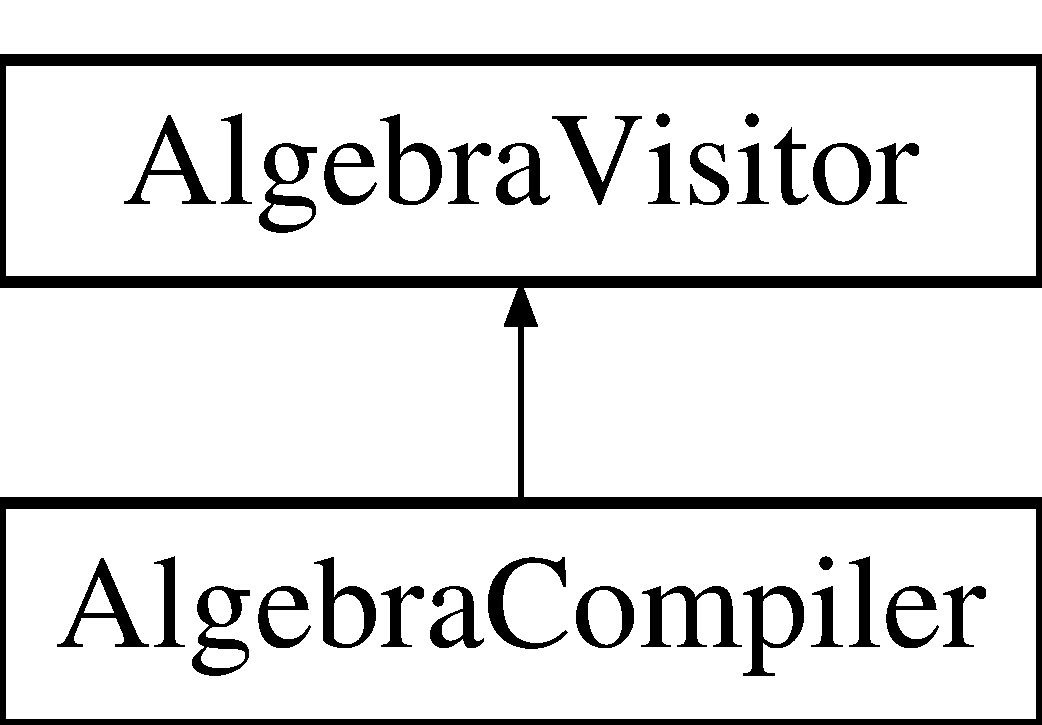
\includegraphics[height=2.000000cm]{class_algebra_compiler}
\end{center}
\end{figure}
\subsection*{Public Member Functions}
\begin{DoxyCompactItemize}
\item 
void \hyperlink{class_algebra_compiler_a5b2f264009e5ed18fcc28c739f67d48a}{visit\+Table} (\hyperlink{class_table}{Table} $\ast$node)
\item 
void \hyperlink{class_algebra_compiler_ab0a1083d8237aeb66e2d8e3c0baff201}{visit\+Sort} (\hyperlink{class_sort}{Sort} $\ast$node)
\item 
void \hyperlink{class_algebra_compiler_aaf1f80df836121f8f8b7abd01e7ac4dd}{visit\+Group} (\hyperlink{class_group}{Group} $\ast$node)
\item 
void \hyperlink{class_algebra_compiler_add29b612e4c40532405924b72f739092}{visit\+Column\+Operations} (\hyperlink{class_column_operations}{Column\+Operations} $\ast$node)
\item 
void \hyperlink{class_algebra_compiler_a22f8846f5665f898e8f67815abe64015}{visit\+Selection} (\hyperlink{class_selection}{Selection} $\ast$node)
\item 
void \hyperlink{class_algebra_compiler_a430ba2ac25d10e94b1408e23def965e6}{visit\+Join} (\hyperlink{class_join}{Join} $\ast$node)
\item 
void \hyperlink{class_algebra_compiler_a4903d8f81d9da91037ce65b6aaeb7fa4}{visit\+Anti\+Join} (\hyperlink{class_anti_join}{Anti\+Join} $\ast$node)
\item 
void \hyperlink{class_algebra_compiler_a6c5170534fba2aa8ed5899f92ceeee8f}{visit\+Union} (\hyperlink{class_union}{Union} $\ast$node)
\item 
void \hyperlink{class_algebra_compiler_acebcb46237fd029f910ae9d06718c1b4}{visit\+Grouped\+Join} (\hyperlink{class_grouped_join}{Grouped\+Join} $\ast$node)
\end{DoxyCompactItemize}
\subsection*{Static Public Member Functions}
\begin{DoxyCompactItemize}
\item 
static void \hyperlink{class_algebra_compiler_a64b17061a41e21787cb35572b60d826d}{update\+Sort\+Parameters} (const \hyperlink{class_possible_sort_parameters}{Possible\+Sort\+Parameters} \&possible\+Sort\+Parameters, std\+::shared\+\_\+ptr$<$ \hyperlink{class_physical_plan}{Physical\+Plan} $>$ \&new\+Plan, std\+::map$<$ int, \hyperlink{class_column_info}{Column\+Info} $>$ \&new\+Columns)
\end{DoxyCompactItemize}
\subsection*{Public Attributes}
\begin{DoxyCompactItemize}
\item 
std\+::vector$<$ std\+::shared\+\_\+ptr\\*
$<$ \hyperlink{class_physical_plan}{Physical\+Plan} $>$ $>$ \hyperlink{class_algebra_compiler_acf3202bd193e4552a1d4fadb6d0b356c}{result}
\end{DoxyCompactItemize}
\subsection*{Static Public Attributes}
\begin{DoxyCompactItemize}
\item 
static const ulong \hyperlink{class_algebra_compiler_ab1a348c2daa3ca8f805f7cec2b35e29d}{N\+U\+M\+B\+E\+R\+\_\+\+O\+F\+\_\+\+P\+L\+A\+N\+S} = 5
\item 
static const ulong \hyperlink{class_algebra_compiler_a75bdf7e239082b0a6c8560ac5a75e72a}{L\+I\+M\+I\+T\+\_\+\+F\+O\+R\+\_\+\+G\+R\+E\+E\+D\+Y\+\_\+\+J\+O\+I\+N\+\_\+\+O\+R\+D\+E\+R\+\_\+\+A\+L\+G\+O\+R\+I\+T\+H\+M} = 5
\item 
static const ulong \hyperlink{class_algebra_compiler_aa67a35b24af1850ef0294e353f8a7184}{M\+A\+X\+\_\+\+H\+E\+A\+P\+\_\+\+S\+I\+Z\+E\+\_\+\+I\+N\+\_\+\+G\+R\+E\+E\+D\+Y\+\_\+\+A\+L\+G\+O\+R\+I\+T\+H\+M} = 20
\end{DoxyCompactItemize}


\subsection{Detailed Description}
\hyperlink{class_algebra_visitor}{Algebra\+Visitor} which compiles relational algebra into physical plan. It uses from down to up method and it saves costant number of best plans for current subtree. 

\subsection{Member Function Documentation}
\hypertarget{class_algebra_compiler_a64b17061a41e21787cb35572b60d826d}{\index{Algebra\+Compiler@{Algebra\+Compiler}!update\+Sort\+Parameters@{update\+Sort\+Parameters}}
\index{update\+Sort\+Parameters@{update\+Sort\+Parameters}!Algebra\+Compiler@{Algebra\+Compiler}}
\subsubsection[{update\+Sort\+Parameters}]{\setlength{\rightskip}{0pt plus 5cm}void Algebra\+Compiler\+::update\+Sort\+Parameters (
\begin{DoxyParamCaption}
\item[{const {\bf Possible\+Sort\+Parameters} \&}]{possible\+Sort\+Parameters, }
\item[{std\+::shared\+\_\+ptr$<$ {\bf Physical\+Plan} $>$ \&}]{new\+Plan, }
\item[{std\+::map$<$ int, {\bf Column\+Info} $>$ \&}]{new\+Columns}
\end{DoxyParamCaption}
)\hspace{0.3cm}{\ttfamily [static]}}}\label{class_algebra_compiler_a64b17061a41e21787cb35572b60d826d}
From possible paramers remove columns, which aren't in new\+Columns and stores them into new\+Plan. 
\begin{DoxyParams}{Parameters}
{\em possible\+Sort\+Parameters} & -\/ parameters to update \\
\hline
{\em new\+Plan} & -\/ \hyperlink{class_physical_plan}{Physical\+Plan}, where to store result \\
\hline
{\em new\+Columns} & -\/ columns which stays in parameters \\
\hline
\end{DoxyParams}
\hypertarget{class_algebra_compiler_a4903d8f81d9da91037ce65b6aaeb7fa4}{\index{Algebra\+Compiler@{Algebra\+Compiler}!visit\+Anti\+Join@{visit\+Anti\+Join}}
\index{visit\+Anti\+Join@{visit\+Anti\+Join}!Algebra\+Compiler@{Algebra\+Compiler}}
\subsubsection[{visit\+Anti\+Join}]{\setlength{\rightskip}{0pt plus 5cm}void Algebra\+Compiler\+::visit\+Anti\+Join (
\begin{DoxyParamCaption}
\item[{{\bf Anti\+Join} $\ast$}]{node}
\end{DoxyParamCaption}
)\hspace{0.3cm}{\ttfamily [virtual]}}}\label{class_algebra_compiler_a4903d8f81d9da91037ce65b6aaeb7fa4}
Visits \hyperlink{class_anti_join}{Anti\+Join} element. 
\begin{DoxyParams}{Parameters}
{\em node} & visited \hyperlink{class_anti_join}{Anti\+Join}. \\
\hline
\end{DoxyParams}


Reimplemented from \hyperlink{class_algebra_visitor_add62415db5f188e572cef1c36faa842e}{Algebra\+Visitor}.

\hypertarget{class_algebra_compiler_add29b612e4c40532405924b72f739092}{\index{Algebra\+Compiler@{Algebra\+Compiler}!visit\+Column\+Operations@{visit\+Column\+Operations}}
\index{visit\+Column\+Operations@{visit\+Column\+Operations}!Algebra\+Compiler@{Algebra\+Compiler}}
\subsubsection[{visit\+Column\+Operations}]{\setlength{\rightskip}{0pt plus 5cm}void Algebra\+Compiler\+::visit\+Column\+Operations (
\begin{DoxyParamCaption}
\item[{{\bf Column\+Operations} $\ast$}]{node}
\end{DoxyParamCaption}
)\hspace{0.3cm}{\ttfamily [virtual]}}}\label{class_algebra_compiler_add29b612e4c40532405924b72f739092}
Visits \hyperlink{class_column_operations}{Column\+Operations} element. 
\begin{DoxyParams}{Parameters}
{\em node} & visited \hyperlink{class_column_operations}{Column\+Operations}. \\
\hline
\end{DoxyParams}


Reimplemented from \hyperlink{class_algebra_visitor_a1109510d982a8e5b90fc56d443109ef9}{Algebra\+Visitor}.

\hypertarget{class_algebra_compiler_aaf1f80df836121f8f8b7abd01e7ac4dd}{\index{Algebra\+Compiler@{Algebra\+Compiler}!visit\+Group@{visit\+Group}}
\index{visit\+Group@{visit\+Group}!Algebra\+Compiler@{Algebra\+Compiler}}
\subsubsection[{visit\+Group}]{\setlength{\rightskip}{0pt plus 5cm}void Algebra\+Compiler\+::visit\+Group (
\begin{DoxyParamCaption}
\item[{{\bf Group} $\ast$}]{node}
\end{DoxyParamCaption}
)\hspace{0.3cm}{\ttfamily [virtual]}}}\label{class_algebra_compiler_aaf1f80df836121f8f8b7abd01e7ac4dd}
Visits \hyperlink{class_group}{Group} element. 
\begin{DoxyParams}{Parameters}
{\em node} & visited \hyperlink{class_group}{Group}. \\
\hline
\end{DoxyParams}


Reimplemented from \hyperlink{class_algebra_visitor_af77bf2aaa949ea27cf992053c43a391b}{Algebra\+Visitor}.

\hypertarget{class_algebra_compiler_acebcb46237fd029f910ae9d06718c1b4}{\index{Algebra\+Compiler@{Algebra\+Compiler}!visit\+Grouped\+Join@{visit\+Grouped\+Join}}
\index{visit\+Grouped\+Join@{visit\+Grouped\+Join}!Algebra\+Compiler@{Algebra\+Compiler}}
\subsubsection[{visit\+Grouped\+Join}]{\setlength{\rightskip}{0pt plus 5cm}void Algebra\+Compiler\+::visit\+Grouped\+Join (
\begin{DoxyParamCaption}
\item[{{\bf Grouped\+Join} $\ast$}]{node}
\end{DoxyParamCaption}
)\hspace{0.3cm}{\ttfamily [virtual]}}}\label{class_algebra_compiler_acebcb46237fd029f910ae9d06718c1b4}
Visits \hyperlink{class_grouped_join}{Grouped\+Join} element. 
\begin{DoxyParams}{Parameters}
{\em node} & visited \hyperlink{class_grouped_join}{Grouped\+Join}. \\
\hline
\end{DoxyParams}


Reimplemented from \hyperlink{class_algebra_visitor_ae92c2f0a465dacc4f42a71e879346c94}{Algebra\+Visitor}.

\hypertarget{class_algebra_compiler_a430ba2ac25d10e94b1408e23def965e6}{\index{Algebra\+Compiler@{Algebra\+Compiler}!visit\+Join@{visit\+Join}}
\index{visit\+Join@{visit\+Join}!Algebra\+Compiler@{Algebra\+Compiler}}
\subsubsection[{visit\+Join}]{\setlength{\rightskip}{0pt plus 5cm}void Algebra\+Compiler\+::visit\+Join (
\begin{DoxyParamCaption}
\item[{{\bf Join} $\ast$}]{node}
\end{DoxyParamCaption}
)\hspace{0.3cm}{\ttfamily [virtual]}}}\label{class_algebra_compiler_a430ba2ac25d10e94b1408e23def965e6}
Visits \hyperlink{class_join}{Join} element. 
\begin{DoxyParams}{Parameters}
{\em node} & visited \hyperlink{class_join}{Join}. \\
\hline
\end{DoxyParams}


Reimplemented from \hyperlink{class_algebra_visitor_a841875539a07c979b912ef44455b873c}{Algebra\+Visitor}.

\hypertarget{class_algebra_compiler_a22f8846f5665f898e8f67815abe64015}{\index{Algebra\+Compiler@{Algebra\+Compiler}!visit\+Selection@{visit\+Selection}}
\index{visit\+Selection@{visit\+Selection}!Algebra\+Compiler@{Algebra\+Compiler}}
\subsubsection[{visit\+Selection}]{\setlength{\rightskip}{0pt plus 5cm}void Algebra\+Compiler\+::visit\+Selection (
\begin{DoxyParamCaption}
\item[{{\bf Selection} $\ast$}]{node}
\end{DoxyParamCaption}
)\hspace{0.3cm}{\ttfamily [virtual]}}}\label{class_algebra_compiler_a22f8846f5665f898e8f67815abe64015}
Visits \hyperlink{class_selection}{Selection} element. 
\begin{DoxyParams}{Parameters}
{\em node} & visited \hyperlink{class_selection}{Selection}. \\
\hline
\end{DoxyParams}


Reimplemented from \hyperlink{class_algebra_visitor_a7d9b0618ac2fdd036abdab27cbb83d40}{Algebra\+Visitor}.

\hypertarget{class_algebra_compiler_ab0a1083d8237aeb66e2d8e3c0baff201}{\index{Algebra\+Compiler@{Algebra\+Compiler}!visit\+Sort@{visit\+Sort}}
\index{visit\+Sort@{visit\+Sort}!Algebra\+Compiler@{Algebra\+Compiler}}
\subsubsection[{visit\+Sort}]{\setlength{\rightskip}{0pt plus 5cm}void Algebra\+Compiler\+::visit\+Sort (
\begin{DoxyParamCaption}
\item[{{\bf Sort} $\ast$}]{node}
\end{DoxyParamCaption}
)\hspace{0.3cm}{\ttfamily [virtual]}}}\label{class_algebra_compiler_ab0a1083d8237aeb66e2d8e3c0baff201}
Visits \hyperlink{class_sort}{Sort} element. 
\begin{DoxyParams}{Parameters}
{\em node} & visited \hyperlink{class_sort}{Sort}. \\
\hline
\end{DoxyParams}


Reimplemented from \hyperlink{class_algebra_visitor_ac350bf44664ce021c0cfec18258a14e8}{Algebra\+Visitor}.

\hypertarget{class_algebra_compiler_a5b2f264009e5ed18fcc28c739f67d48a}{\index{Algebra\+Compiler@{Algebra\+Compiler}!visit\+Table@{visit\+Table}}
\index{visit\+Table@{visit\+Table}!Algebra\+Compiler@{Algebra\+Compiler}}
\subsubsection[{visit\+Table}]{\setlength{\rightskip}{0pt plus 5cm}void Algebra\+Compiler\+::visit\+Table (
\begin{DoxyParamCaption}
\item[{{\bf Table} $\ast$}]{node}
\end{DoxyParamCaption}
)\hspace{0.3cm}{\ttfamily [virtual]}}}\label{class_algebra_compiler_a5b2f264009e5ed18fcc28c739f67d48a}
Visits \hyperlink{class_table}{Table} element. 
\begin{DoxyParams}{Parameters}
{\em node} & visited \hyperlink{class_table}{Table}. \\
\hline
\end{DoxyParams}


Reimplemented from \hyperlink{class_algebra_visitor_ac14f3c3c195373e3bae5d01d04f1ea09}{Algebra\+Visitor}.

\hypertarget{class_algebra_compiler_a6c5170534fba2aa8ed5899f92ceeee8f}{\index{Algebra\+Compiler@{Algebra\+Compiler}!visit\+Union@{visit\+Union}}
\index{visit\+Union@{visit\+Union}!Algebra\+Compiler@{Algebra\+Compiler}}
\subsubsection[{visit\+Union}]{\setlength{\rightskip}{0pt plus 5cm}void Algebra\+Compiler\+::visit\+Union (
\begin{DoxyParamCaption}
\item[{{\bf Union} $\ast$}]{node}
\end{DoxyParamCaption}
)\hspace{0.3cm}{\ttfamily [virtual]}}}\label{class_algebra_compiler_a6c5170534fba2aa8ed5899f92ceeee8f}
Visits \hyperlink{class_union}{Union} element. 
\begin{DoxyParams}{Parameters}
{\em node} & visited \hyperlink{class_union}{Union}. \\
\hline
\end{DoxyParams}


Reimplemented from \hyperlink{class_algebra_visitor_a681732083691701f0e9c10980392dd3c}{Algebra\+Visitor}.



\subsection{Member Data Documentation}
\hypertarget{class_algebra_compiler_a75bdf7e239082b0a6c8560ac5a75e72a}{\index{Algebra\+Compiler@{Algebra\+Compiler}!L\+I\+M\+I\+T\+\_\+\+F\+O\+R\+\_\+\+G\+R\+E\+E\+D\+Y\+\_\+\+J\+O\+I\+N\+\_\+\+O\+R\+D\+E\+R\+\_\+\+A\+L\+G\+O\+R\+I\+T\+H\+M@{L\+I\+M\+I\+T\+\_\+\+F\+O\+R\+\_\+\+G\+R\+E\+E\+D\+Y\+\_\+\+J\+O\+I\+N\+\_\+\+O\+R\+D\+E\+R\+\_\+\+A\+L\+G\+O\+R\+I\+T\+H\+M}}
\index{L\+I\+M\+I\+T\+\_\+\+F\+O\+R\+\_\+\+G\+R\+E\+E\+D\+Y\+\_\+\+J\+O\+I\+N\+\_\+\+O\+R\+D\+E\+R\+\_\+\+A\+L\+G\+O\+R\+I\+T\+H\+M@{L\+I\+M\+I\+T\+\_\+\+F\+O\+R\+\_\+\+G\+R\+E\+E\+D\+Y\+\_\+\+J\+O\+I\+N\+\_\+\+O\+R\+D\+E\+R\+\_\+\+A\+L\+G\+O\+R\+I\+T\+H\+M}!Algebra\+Compiler@{Algebra\+Compiler}}
\subsubsection[{L\+I\+M\+I\+T\+\_\+\+F\+O\+R\+\_\+\+G\+R\+E\+E\+D\+Y\+\_\+\+J\+O\+I\+N\+\_\+\+O\+R\+D\+E\+R\+\_\+\+A\+L\+G\+O\+R\+I\+T\+H\+M}]{\setlength{\rightskip}{0pt plus 5cm}const ulong Algebra\+Compiler\+::\+L\+I\+M\+I\+T\+\_\+\+F\+O\+R\+\_\+\+G\+R\+E\+E\+D\+Y\+\_\+\+J\+O\+I\+N\+\_\+\+O\+R\+D\+E\+R\+\_\+\+A\+L\+G\+O\+R\+I\+T\+H\+M = 5\hspace{0.3cm}{\ttfamily [static]}}}\label{class_algebra_compiler_a75bdf7e239082b0a6c8560ac5a75e72a}
Determines maximal number of inputs in group join to uses brute force join order algorithm. Otherwise greedy algorithm is used. \hypertarget{class_algebra_compiler_aa67a35b24af1850ef0294e353f8a7184}{\index{Algebra\+Compiler@{Algebra\+Compiler}!M\+A\+X\+\_\+\+H\+E\+A\+P\+\_\+\+S\+I\+Z\+E\+\_\+\+I\+N\+\_\+\+G\+R\+E\+E\+D\+Y\+\_\+\+A\+L\+G\+O\+R\+I\+T\+H\+M@{M\+A\+X\+\_\+\+H\+E\+A\+P\+\_\+\+S\+I\+Z\+E\+\_\+\+I\+N\+\_\+\+G\+R\+E\+E\+D\+Y\+\_\+\+A\+L\+G\+O\+R\+I\+T\+H\+M}}
\index{M\+A\+X\+\_\+\+H\+E\+A\+P\+\_\+\+S\+I\+Z\+E\+\_\+\+I\+N\+\_\+\+G\+R\+E\+E\+D\+Y\+\_\+\+A\+L\+G\+O\+R\+I\+T\+H\+M@{M\+A\+X\+\_\+\+H\+E\+A\+P\+\_\+\+S\+I\+Z\+E\+\_\+\+I\+N\+\_\+\+G\+R\+E\+E\+D\+Y\+\_\+\+A\+L\+G\+O\+R\+I\+T\+H\+M}!Algebra\+Compiler@{Algebra\+Compiler}}
\subsubsection[{M\+A\+X\+\_\+\+H\+E\+A\+P\+\_\+\+S\+I\+Z\+E\+\_\+\+I\+N\+\_\+\+G\+R\+E\+E\+D\+Y\+\_\+\+A\+L\+G\+O\+R\+I\+T\+H\+M}]{\setlength{\rightskip}{0pt plus 5cm}const ulong Algebra\+Compiler\+::\+M\+A\+X\+\_\+\+H\+E\+A\+P\+\_\+\+S\+I\+Z\+E\+\_\+\+I\+N\+\_\+\+G\+R\+E\+E\+D\+Y\+\_\+\+A\+L\+G\+O\+R\+I\+T\+H\+M = 20\hspace{0.3cm}{\ttfamily [static]}}}\label{class_algebra_compiler_aa67a35b24af1850ef0294e353f8a7184}
Determines how many plans can be stored in greddy join algorithm. \hypertarget{class_algebra_compiler_ab1a348c2daa3ca8f805f7cec2b35e29d}{\index{Algebra\+Compiler@{Algebra\+Compiler}!N\+U\+M\+B\+E\+R\+\_\+\+O\+F\+\_\+\+P\+L\+A\+N\+S@{N\+U\+M\+B\+E\+R\+\_\+\+O\+F\+\_\+\+P\+L\+A\+N\+S}}
\index{N\+U\+M\+B\+E\+R\+\_\+\+O\+F\+\_\+\+P\+L\+A\+N\+S@{N\+U\+M\+B\+E\+R\+\_\+\+O\+F\+\_\+\+P\+L\+A\+N\+S}!Algebra\+Compiler@{Algebra\+Compiler}}
\subsubsection[{N\+U\+M\+B\+E\+R\+\_\+\+O\+F\+\_\+\+P\+L\+A\+N\+S}]{\setlength{\rightskip}{0pt plus 5cm}const ulong Algebra\+Compiler\+::\+N\+U\+M\+B\+E\+R\+\_\+\+O\+F\+\_\+\+P\+L\+A\+N\+S = 5\hspace{0.3cm}{\ttfamily [static]}}}\label{class_algebra_compiler_ab1a348c2daa3ca8f805f7cec2b35e29d}
Determines what number of plans are used from visited subtree. \hypertarget{class_algebra_compiler_acf3202bd193e4552a1d4fadb6d0b356c}{\index{Algebra\+Compiler@{Algebra\+Compiler}!result@{result}}
\index{result@{result}!Algebra\+Compiler@{Algebra\+Compiler}}
\subsubsection[{result}]{\setlength{\rightskip}{0pt plus 5cm}std\+::vector$<$std\+::shared\+\_\+ptr$<${\bf Physical\+Plan}$>$ $>$ Algebra\+Compiler\+::result}}\label{class_algebra_compiler_acf3202bd193e4552a1d4fadb6d0b356c}
Stores plans after processing subtree. 

The documentation for this class was generated from the following files\+:\begin{DoxyCompactItemize}
\item 
C\+:/\+Users/\+Marcel/\+Documents/\+Visual Studio 2012/\+Projects/\+Relational\+Query\+Evaluator/\+Relational\+Query\+Evaluator/Algebra\+Visitors.\+h\item 
C\+:/\+Users/\+Marcel/\+Documents/\+Visual Studio 2012/\+Projects/\+Relational\+Query\+Evaluator/\+Relational\+Query\+Evaluator/Algebra\+Compiler.\+cpp\end{DoxyCompactItemize}

\hypertarget{class_algebra_node_base}{\section{Algebra\+Node\+Base Class Reference}
\label{class_algebra_node_base}\index{Algebra\+Node\+Base@{Algebra\+Node\+Base}}
}


{\ttfamily \#include $<$Algebra.\+h$>$}

Inheritance diagram for Algebra\+Node\+Base\+:\begin{figure}[H]
\begin{center}
\leavevmode
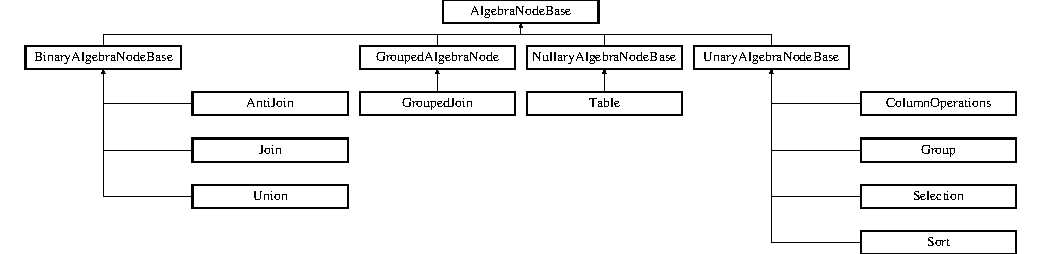
\includegraphics[height=3.414634cm]{class_algebra_node_base}
\end{center}
\end{figure}
\subsection*{Public Member Functions}
\begin{DoxyCompactItemize}
\item 
\hypertarget{class_algebra_node_base_a19f93dd9f8b3da0a216a37f2ceb61ebe}{\hyperlink{class_algebra_node_base}{Algebra\+Node\+Base} $\ast$ {\bfseries construct\+Children} (D\+O\+M\+Element $\ast$node)}\label{class_algebra_node_base_a19f93dd9f8b3da0a216a37f2ceb61ebe}

\item 
\hypertarget{class_algebra_node_base_a33bee3ec6fe1eb4228c0471c95c90d66}{virtual void {\bfseries accept} (\hyperlink{class_algebra_visitor}{Algebra\+Visitor} \&v)=0}\label{class_algebra_node_base_a33bee3ec6fe1eb4228c0471c95c90d66}

\item 
\hypertarget{class_algebra_node_base_aa9bdd02b0ddf793bda18bd146ccacb0d}{virtual std\+::shared\+\_\+ptr\\*
$<$ \hyperlink{class_algebra_node_base}{Algebra\+Node\+Base} $>$ {\bfseries replace\+Child} (\hyperlink{class_algebra_node_base}{Algebra\+Node\+Base} $\ast$old\+Child, std\+::shared\+\_\+ptr$<$ \hyperlink{class_algebra_node_base}{Algebra\+Node\+Base} $>$ \&new\+Child)=0}\label{class_algebra_node_base_aa9bdd02b0ddf793bda18bd146ccacb0d}

\end{DoxyCompactItemize}
\subsection*{Public Attributes}
\begin{DoxyCompactItemize}
\item 
\hypertarget{class_algebra_node_base_ac59c590aea4f109c7fab18f714c588c1}{std\+::map$<$ int, \hyperlink{class_column_info}{Column\+Info} $>$ {\bfseries output\+Columns}}\label{class_algebra_node_base_ac59c590aea4f109c7fab18f714c588c1}

\item 
\hypertarget{class_algebra_node_base_a5b2834cce900dec172763d4ef4b38f66}{\hyperlink{class_algebra_node_base}{Algebra\+Node\+Base} $\ast$ {\bfseries parent}}\label{class_algebra_node_base_a5b2834cce900dec172763d4ef4b38f66}

\end{DoxyCompactItemize}


\subsection{Detailed Description}
... Qt style comments ... 

The documentation for this class was generated from the following files\+:\begin{DoxyCompactItemize}
\item 
C\+:/\+Users/\+Marcel/\+Documents/\+Visual Studio 2012/\+Projects/\+Relational\+Query\+Evaluator/\+Relational\+Query\+Evaluator/Algebra.\+h\item 
C\+:/\+Users/\+Marcel/\+Documents/\+Visual Studio 2012/\+Projects/\+Relational\+Query\+Evaluator/\+Relational\+Query\+Evaluator/Algebra.\+cpp\end{DoxyCompactItemize}

\hypertarget{class_algebra_visitor}{\section{Algebra\+Visitor Class Reference}
\label{class_algebra_visitor}\index{Algebra\+Visitor@{Algebra\+Visitor}}
}
Inheritance diagram for Algebra\+Visitor\+:\begin{figure}[H]
\begin{center}
\leavevmode
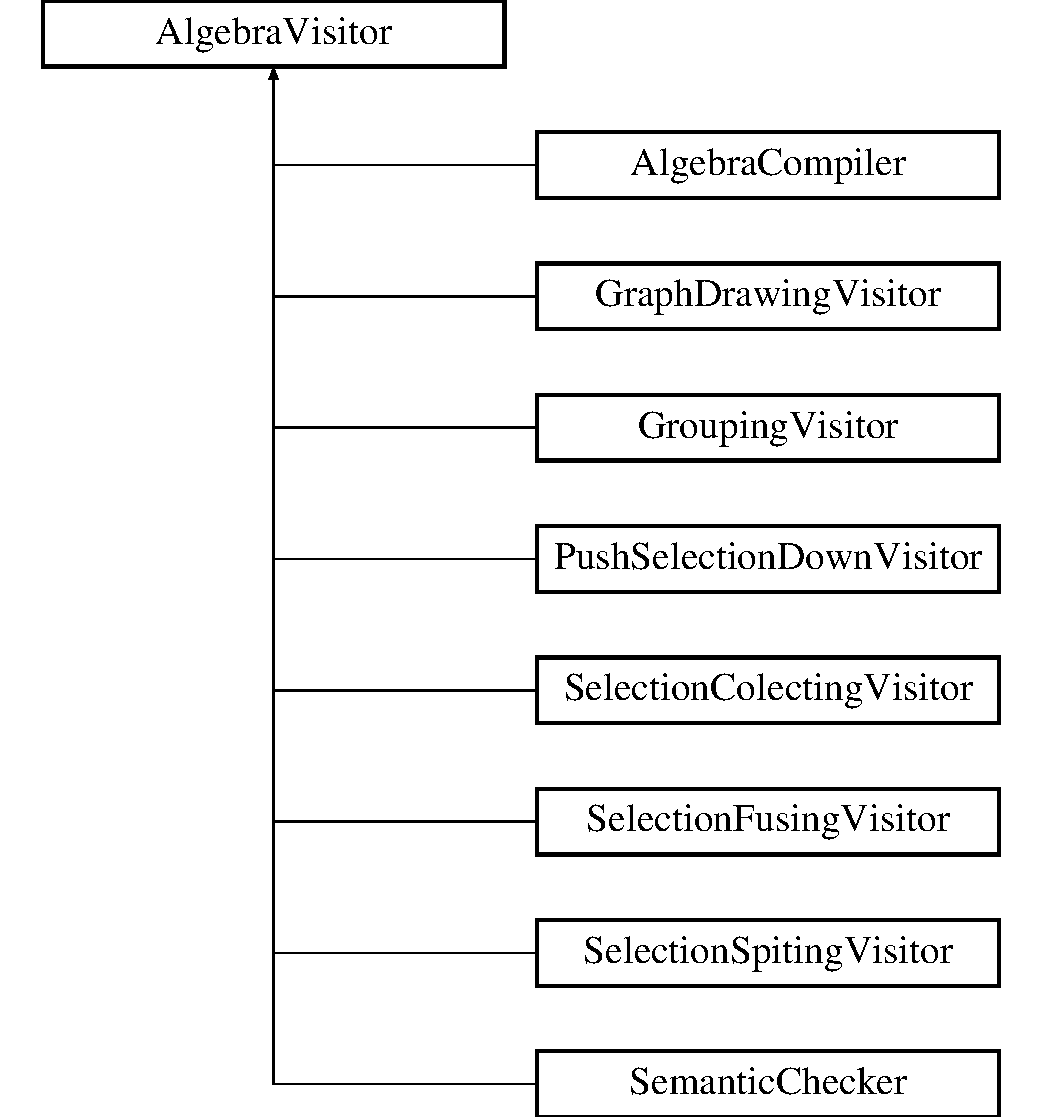
\includegraphics[height=9.000000cm]{class_algebra_visitor}
\end{center}
\end{figure}
\subsection*{Public Member Functions}
\begin{DoxyCompactItemize}
\item 
\hypertarget{class_algebra_visitor_a97257e8a65f77f30540b1223d92127fb}{virtual void {\bfseries visit\+Algebra\+Node\+Base} (\hyperlink{class_algebra_node_base}{Algebra\+Node\+Base} $\ast$node)}\label{class_algebra_visitor_a97257e8a65f77f30540b1223d92127fb}

\item 
\hypertarget{class_algebra_visitor_a371a822b60caab82b78c5750eff67b4b}{virtual void {\bfseries visit\+Unary\+Algebra\+Node\+Base} (\hyperlink{class_unary_algebra_node_base}{Unary\+Algebra\+Node\+Base} $\ast$node)}\label{class_algebra_visitor_a371a822b60caab82b78c5750eff67b4b}

\item 
\hypertarget{class_algebra_visitor_a00b2a6a2fb076160c0a8f713dd48d6d1}{virtual void {\bfseries visit\+Binary\+Algebra\+Node\+Base} (\hyperlink{class_binary_algebra_node_base}{Binary\+Algebra\+Node\+Base} $\ast$node)}\label{class_algebra_visitor_a00b2a6a2fb076160c0a8f713dd48d6d1}

\item 
\hypertarget{class_algebra_visitor_a5b5642743b1985cc5fd1e12002972388}{virtual void {\bfseries visit\+Nullary\+Algebra\+Node\+Base} (\hyperlink{class_nullary_algebra_node_base}{Nullary\+Algebra\+Node\+Base} $\ast$node)}\label{class_algebra_visitor_a5b5642743b1985cc5fd1e12002972388}

\item 
\hypertarget{class_algebra_visitor_a21ccc9b452a5c842d91cab7ec0855cfe}{virtual void {\bfseries visit\+Grouped\+Algebra\+Node} (\hyperlink{class_grouped_algebra_node}{Grouped\+Algebra\+Node} $\ast$node)}\label{class_algebra_visitor_a21ccc9b452a5c842d91cab7ec0855cfe}

\item 
\hypertarget{class_algebra_visitor_ac14f3c3c195373e3bae5d01d04f1ea09}{virtual void {\bfseries visit\+Table} (\hyperlink{class_table}{Table} $\ast$node)}\label{class_algebra_visitor_ac14f3c3c195373e3bae5d01d04f1ea09}

\item 
\hypertarget{class_algebra_visitor_ac350bf44664ce021c0cfec18258a14e8}{virtual void {\bfseries visit\+Sort} (\hyperlink{class_sort}{Sort} $\ast$node)}\label{class_algebra_visitor_ac350bf44664ce021c0cfec18258a14e8}

\item 
\hypertarget{class_algebra_visitor_af77bf2aaa949ea27cf992053c43a391b}{virtual void {\bfseries visit\+Group} (\hyperlink{class_group}{Group} $\ast$node)}\label{class_algebra_visitor_af77bf2aaa949ea27cf992053c43a391b}

\item 
\hypertarget{class_algebra_visitor_a1109510d982a8e5b90fc56d443109ef9}{virtual void {\bfseries visit\+Column\+Operations} (\hyperlink{class_column_operations}{Column\+Operations} $\ast$node)}\label{class_algebra_visitor_a1109510d982a8e5b90fc56d443109ef9}

\item 
\hypertarget{class_algebra_visitor_a7d9b0618ac2fdd036abdab27cbb83d40}{virtual void {\bfseries visit\+Selection} (\hyperlink{class_selection}{Selection} $\ast$node)}\label{class_algebra_visitor_a7d9b0618ac2fdd036abdab27cbb83d40}

\item 
\hypertarget{class_algebra_visitor_a841875539a07c979b912ef44455b873c}{virtual void {\bfseries visit\+Join} (\hyperlink{class_join}{Join} $\ast$node)}\label{class_algebra_visitor_a841875539a07c979b912ef44455b873c}

\item 
\hypertarget{class_algebra_visitor_add62415db5f188e572cef1c36faa842e}{virtual void {\bfseries visit\+Anti\+Join} (\hyperlink{class_anti_join}{Anti\+Join} $\ast$node)}\label{class_algebra_visitor_add62415db5f188e572cef1c36faa842e}

\item 
\hypertarget{class_algebra_visitor_a681732083691701f0e9c10980392dd3c}{virtual void {\bfseries visit\+Union} (\hyperlink{class_union}{Union} $\ast$node)}\label{class_algebra_visitor_a681732083691701f0e9c10980392dd3c}

\item 
\hypertarget{class_algebra_visitor_ae92c2f0a465dacc4f42a71e879346c94}{virtual void {\bfseries visit\+Grouped\+Join} (\hyperlink{class_grouped_join}{Grouped\+Join} $\ast$node)}\label{class_algebra_visitor_ae92c2f0a465dacc4f42a71e879346c94}

\end{DoxyCompactItemize}
\subsection*{Static Public Member Functions}
\begin{DoxyCompactItemize}
\item 
\hypertarget{class_algebra_visitor_aa8f4149dca3babdefa323050bb6e82f9}{static void {\bfseries serialize\+Expression} (std\+::shared\+\_\+ptr$<$ \hyperlink{class_expression}{Expression} $>$ \&condition, std\+::vector$<$ std\+::shared\+\_\+ptr$<$ \hyperlink{class_expression}{Expression} $>$ $>$ \&result)}\label{class_algebra_visitor_aa8f4149dca3babdefa323050bb6e82f9}

\item 
\hypertarget{class_algebra_visitor_a20d1215ba30361d19d0317a939a9b860}{static std\+::shared\+\_\+ptr\\*
$<$ \hyperlink{class_expression}{Expression} $>$ {\bfseries deserialize\+Expression} (const std\+::vector$<$ std\+::shared\+\_\+ptr$<$ \hyperlink{class_expression}{Expression} $>$ $>$ \&condition)}\label{class_algebra_visitor_a20d1215ba30361d19d0317a939a9b860}

\item 
\hypertarget{class_algebra_visitor_a78119cf006ac64137b8c29223ab77885}{static void {\bfseries remove\+Selection} (\hyperlink{class_selection}{Selection} $\ast$node)}\label{class_algebra_visitor_a78119cf006ac64137b8c29223ab77885}

\item 
\hypertarget{class_algebra_visitor_adbcb61f031cfc4808d150b076f6aa63d}{static void {\bfseries insert\+Selection} (\hyperlink{class_algebra_node_base}{Algebra\+Node\+Base} $\ast$node, std\+::shared\+\_\+ptr$<$ \hyperlink{class_selection}{Selection} $>$ \&selection)}\label{class_algebra_visitor_adbcb61f031cfc4808d150b076f6aa63d}

\end{DoxyCompactItemize}


The documentation for this class was generated from the following files\+:\begin{DoxyCompactItemize}
\item 
C\+:/\+Users/\+Marcel/\+Documents/\+Visual Studio 2012/\+Projects/\+Relational\+Query\+Evaluator/\+Relational\+Query\+Evaluator/Algebra\+Visitors.\+h\item 
C\+:/\+Users/\+Marcel/\+Documents/\+Visual Studio 2012/\+Projects/\+Relational\+Query\+Evaluator/\+Relational\+Query\+Evaluator/Algebra\+Visitors.\+cpp\end{DoxyCompactItemize}

\hypertarget{class_anti_join}{\section{Anti\+Join Class Reference}
\label{class_anti_join}\index{Anti\+Join@{Anti\+Join}}
}


{\ttfamily \#include $<$Algebra.\+h$>$}

Inheritance diagram for Anti\+Join\+:\begin{figure}[H]
\begin{center}
\leavevmode
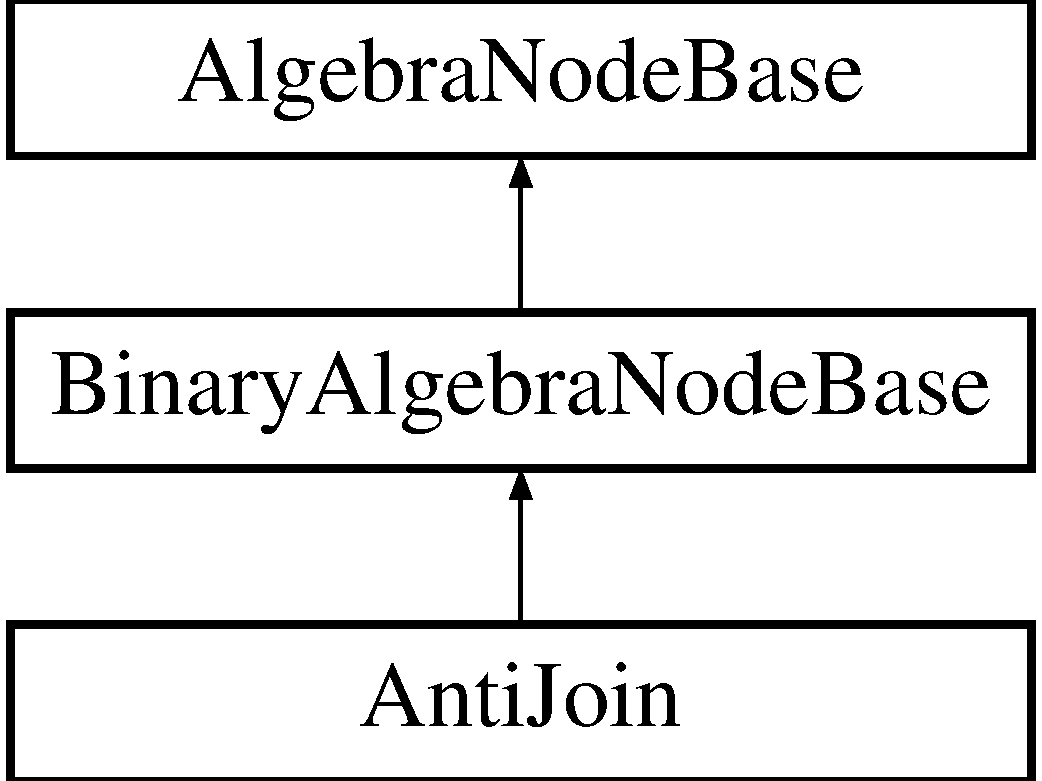
\includegraphics[height=3.000000cm]{class_anti_join}
\end{center}
\end{figure}
\subsection*{Public Member Functions}
\begin{DoxyCompactItemize}
\item 
\hyperlink{class_anti_join_a5cc6257a7d3b85eebc2326e2a5996dec}{Anti\+Join} (D\+O\+M\+Element $\ast$element)
\item 
void \hyperlink{class_anti_join_a95d753b1ed036be43a4fe00b40b775cf}{accept} (\hyperlink{class_algebra_visitor}{Algebra\+Visitor} \&v)
\end{DoxyCompactItemize}
\subsection*{Public Attributes}
\begin{DoxyCompactItemize}
\item 
std\+::shared\+\_\+ptr$<$ \hyperlink{class_expression}{Expression} $>$ \hyperlink{class_anti_join_a55e3da2742c4a24af7eee18cc5309206}{condition}
\item 
std\+::vector$<$ \hyperlink{class_join_column_info}{Join\+Column\+Info} $>$ \hyperlink{class_anti_join_af033e50994f2155c9f33926ec2ecd375}{output\+Join\+Columns}
\end{DoxyCompactItemize}


\subsection{Detailed Description}
Represents algebraic operation antijoin. Antijoin is basicly generalized difference but the columns doesn't have to be same. 

\subsection{Constructor \& Destructor Documentation}
\hypertarget{class_anti_join_a5cc6257a7d3b85eebc2326e2a5996dec}{\index{Anti\+Join@{Anti\+Join}!Anti\+Join@{Anti\+Join}}
\index{Anti\+Join@{Anti\+Join}!Anti\+Join@{Anti\+Join}}
\subsubsection[{Anti\+Join}]{\setlength{\rightskip}{0pt plus 5cm}Anti\+Join\+::\+Anti\+Join (
\begin{DoxyParamCaption}
\item[{D\+O\+M\+Element $\ast$}]{element}
\end{DoxyParamCaption}
)}}\label{class_anti_join_a5cc6257a7d3b85eebc2326e2a5996dec}
Create the instance of \hyperlink{class_anti_join}{Anti\+Join}. 
\begin{DoxyParams}{Parameters}
{\em element} & representing input node. \\
\hline
\end{DoxyParams}


\subsection{Member Function Documentation}
\hypertarget{class_anti_join_a95d753b1ed036be43a4fe00b40b775cf}{\index{Anti\+Join@{Anti\+Join}!accept@{accept}}
\index{accept@{accept}!Anti\+Join@{Anti\+Join}}
\subsubsection[{accept}]{\setlength{\rightskip}{0pt plus 5cm}void Anti\+Join\+::accept (
\begin{DoxyParamCaption}
\item[{{\bf Algebra\+Visitor} \&}]{v}
\end{DoxyParamCaption}
)\hspace{0.3cm}{\ttfamily [virtual]}}}\label{class_anti_join_a95d753b1ed036be43a4fe00b40b775cf}
Method for calling visit\mbox{[}node\mbox{]} on given \hyperlink{class_algebra_visitor}{Algebra\+Visitor} 
\begin{DoxyParams}{Parameters}
{\em v} & \hyperlink{class_algebra_visitor}{Algebra\+Visitor}, on which to call function \\
\hline
\end{DoxyParams}


Implements \hyperlink{class_binary_algebra_node_base_ab6521a638b418e4f0939270bab77b901}{Binary\+Algebra\+Node\+Base}.



\subsection{Member Data Documentation}
\hypertarget{class_anti_join_a55e3da2742c4a24af7eee18cc5309206}{\index{Anti\+Join@{Anti\+Join}!condition@{condition}}
\index{condition@{condition}!Anti\+Join@{Anti\+Join}}
\subsubsection[{condition}]{\setlength{\rightskip}{0pt plus 5cm}std\+::shared\+\_\+ptr$<${\bf Expression}$>$ Anti\+Join\+::condition}}\label{class_anti_join_a55e3da2742c4a24af7eee18cc5309206}
Condition for antijoin joining. \hypertarget{class_anti_join_af033e50994f2155c9f33926ec2ecd375}{\index{Anti\+Join@{Anti\+Join}!output\+Join\+Columns@{output\+Join\+Columns}}
\index{output\+Join\+Columns@{output\+Join\+Columns}!Anti\+Join@{Anti\+Join}}
\subsubsection[{output\+Join\+Columns}]{\setlength{\rightskip}{0pt plus 5cm}std\+::vector$<${\bf Join\+Column\+Info}$>$ Anti\+Join\+::output\+Join\+Columns}}\label{class_anti_join_af033e50994f2155c9f33926ec2ecd375}
list of output columns from join 

The documentation for this class was generated from the following files\+:\begin{DoxyCompactItemize}
\item 
C\+:/\+Users/\+Marcel/\+Documents/\+Visual Studio 2012/\+Projects/\+Relational\+Query\+Evaluator/\+Relational\+Query\+Evaluator/Algebra.\+h\item 
C\+:/\+Users/\+Marcel/\+Documents/\+Visual Studio 2012/\+Projects/\+Relational\+Query\+Evaluator/\+Relational\+Query\+Evaluator/Algebra.\+cpp\end{DoxyCompactItemize}

\hypertarget{class_binary_algebra_node_base}{\section{Binary\+Algebra\+Node\+Base Class Reference}
\label{class_binary_algebra_node_base}\index{Binary\+Algebra\+Node\+Base@{Binary\+Algebra\+Node\+Base}}
}
Inheritance diagram for Binary\+Algebra\+Node\+Base\+:\begin{figure}[H]
\begin{center}
\leavevmode
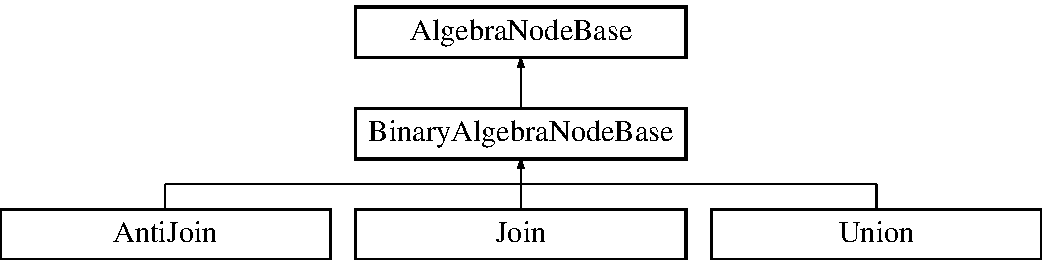
\includegraphics[height=3.000000cm]{class_binary_algebra_node_base}
\end{center}
\end{figure}
\subsection*{Public Member Functions}
\begin{DoxyCompactItemize}
\item 
\hypertarget{class_binary_algebra_node_base_a0a44a290bb4c433b83f58d948240a0d0}{{\bfseries Binary\+Algebra\+Node\+Base} (D\+O\+M\+Element $\ast$element)}\label{class_binary_algebra_node_base_a0a44a290bb4c433b83f58d948240a0d0}

\item 
\hypertarget{class_binary_algebra_node_base_ab6521a638b418e4f0939270bab77b901}{virtual void {\bfseries accept} (\hyperlink{class_algebra_visitor}{Algebra\+Visitor} \&v)=0}\label{class_binary_algebra_node_base_ab6521a638b418e4f0939270bab77b901}

\item 
\hypertarget{class_binary_algebra_node_base_a266f8e4526337e86f97ebeabb326be22}{void {\bfseries construct\+Join\+Parameters} (D\+O\+M\+Element $\ast$node, std\+::shared\+\_\+ptr$<$ \hyperlink{class_expression}{Expression} $>$ \&condition, std\+::vector$<$ \hyperlink{class_join_column_info}{Join\+Column\+Info} $>$ \&output\+Columns)}\label{class_binary_algebra_node_base_a266f8e4526337e86f97ebeabb326be22}

\item 
\hypertarget{class_binary_algebra_node_base_a6e466b62966a9851c3c34e1fb588a496}{std\+::shared\+\_\+ptr$<$ \hyperlink{class_algebra_node_base}{Algebra\+Node\+Base} $>$ {\bfseries replace\+Child} (\hyperlink{class_algebra_node_base}{Algebra\+Node\+Base} $\ast$old\+Child, std\+::shared\+\_\+ptr$<$ \hyperlink{class_algebra_node_base}{Algebra\+Node\+Base} $>$ \&new\+Child)}\label{class_binary_algebra_node_base_a6e466b62966a9851c3c34e1fb588a496}

\end{DoxyCompactItemize}
\subsection*{Public Attributes}
\begin{DoxyCompactItemize}
\item 
\hypertarget{class_binary_algebra_node_base_ab62ff77c5d90bd941b07a6f34e39f14b}{std\+::shared\+\_\+ptr$<$ \hyperlink{class_algebra_node_base}{Algebra\+Node\+Base} $>$ {\bfseries left\+Child}}\label{class_binary_algebra_node_base_ab62ff77c5d90bd941b07a6f34e39f14b}

\item 
\hypertarget{class_binary_algebra_node_base_ac97784ae724c411daca8b17664ce1122}{std\+::shared\+\_\+ptr$<$ \hyperlink{class_algebra_node_base}{Algebra\+Node\+Base} $>$ {\bfseries right\+Child}}\label{class_binary_algebra_node_base_ac97784ae724c411daca8b17664ce1122}

\end{DoxyCompactItemize}


The documentation for this class was generated from the following files\+:\begin{DoxyCompactItemize}
\item 
C\+:/\+Users/\+Marcel/\+Documents/\+Visual Studio 2012/\+Projects/\+Relational\+Query\+Evaluator/\+Relational\+Query\+Evaluator/Algebra.\+h\item 
C\+:/\+Users/\+Marcel/\+Documents/\+Visual Studio 2012/\+Projects/\+Relational\+Query\+Evaluator/\+Relational\+Query\+Evaluator/Algebra.\+cpp\end{DoxyCompactItemize}

\hypertarget{class_binary_expression}{\section{Binary\+Expression Class Reference}
\label{class_binary_expression}\index{Binary\+Expression@{Binary\+Expression}}
}
Inheritance diagram for Binary\+Expression\+:\begin{figure}[H]
\begin{center}
\leavevmode
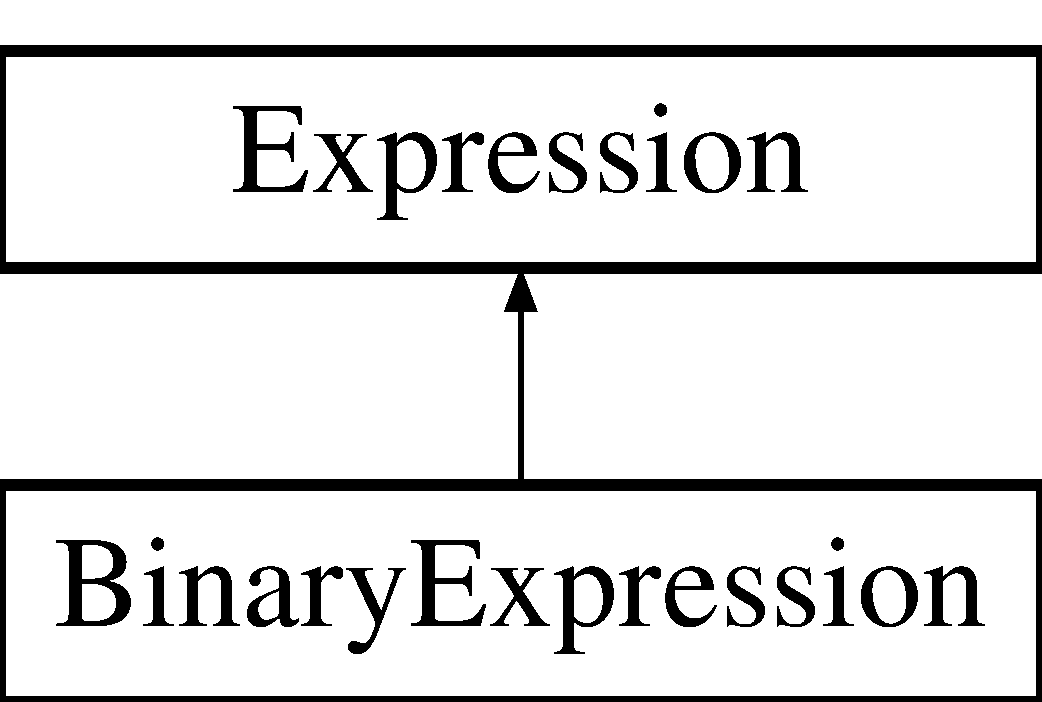
\includegraphics[height=2.000000cm]{class_binary_expression}
\end{center}
\end{figure}
\subsection*{Public Member Functions}
\begin{DoxyCompactItemize}
\item 
\hypertarget{class_binary_expression_a5d19c8f759e63c10af90f1951b5a760d}{{\bfseries Binary\+Expression} (D\+O\+M\+Element $\ast$node, Binary\+Operator op)}\label{class_binary_expression_a5d19c8f759e63c10af90f1951b5a760d}

\item 
\hypertarget{class_binary_expression_af3c15a9d05697963ebac1e010e894c04}{{\bfseries Binary\+Expression} (std\+::shared\+\_\+ptr$<$ \hyperlink{class_expression}{Expression} $>$ \&left\+Child, std\+::shared\+\_\+ptr$<$ \hyperlink{class_expression}{Expression} $>$ \&right\+Child, Binary\+Operator op)}\label{class_binary_expression_af3c15a9d05697963ebac1e010e894c04}

\item 
\hypertarget{class_binary_expression_a12ea9a0735a8809b01059988b6466d7c}{void {\bfseries accept} (\hyperlink{class_expression_visitor_base}{Expression\+Visitor\+Base} \&v)}\label{class_binary_expression_a12ea9a0735a8809b01059988b6466d7c}

\item 
\hypertarget{class_binary_expression_a7ff9236432aef24bca655ab45cf475f2}{void {\bfseries replace\+Child} (\hyperlink{class_expression}{Expression} $\ast$old\+Child, std\+::shared\+\_\+ptr$<$ \hyperlink{class_expression}{Expression} $>$ new\+Child)}\label{class_binary_expression_a7ff9236432aef24bca655ab45cf475f2}

\end{DoxyCompactItemize}
\subsection*{Public Attributes}
\begin{DoxyCompactItemize}
\item 
\hypertarget{class_binary_expression_ac3926bbcc2ed7bb00eca10b4d4e590d2}{Binary\+Operator {\bfseries operation}}\label{class_binary_expression_ac3926bbcc2ed7bb00eca10b4d4e590d2}

\item 
\hypertarget{class_binary_expression_a2388939b40f93649cfd3c531b181025e}{std\+::shared\+\_\+ptr$<$ \hyperlink{class_expression}{Expression} $>$ {\bfseries left\+Child}}\label{class_binary_expression_a2388939b40f93649cfd3c531b181025e}

\item 
\hypertarget{class_binary_expression_a97803d6333b2fbe6098491136a1445af}{std\+::shared\+\_\+ptr$<$ \hyperlink{class_expression}{Expression} $>$ {\bfseries right\+Child}}\label{class_binary_expression_a97803d6333b2fbe6098491136a1445af}

\end{DoxyCompactItemize}
\subsection*{Additional Inherited Members}


The documentation for this class was generated from the following files\+:\begin{DoxyCompactItemize}
\item 
C\+:/\+Users/\+Marcel/\+Documents/\+Visual Studio 2012/\+Projects/\+Relational\+Query\+Evaluator/\+Relational\+Query\+Evaluator/Expressions.\+h\item 
C\+:/\+Users/\+Marcel/\+Documents/\+Visual Studio 2012/\+Projects/\+Relational\+Query\+Evaluator/\+Relational\+Query\+Evaluator/Expressions.\+cpp\end{DoxyCompactItemize}

\hypertarget{class_binary_physical_operator}{\section{Binary\+Physical\+Operator Class Reference}
\label{class_binary_physical_operator}\index{Binary\+Physical\+Operator@{Binary\+Physical\+Operator}}
}


{\ttfamily \#include $<$Physical\+Operator.\+h$>$}

Inheritance diagram for Binary\+Physical\+Operator\+:\begin{figure}[H]
\begin{center}
\leavevmode
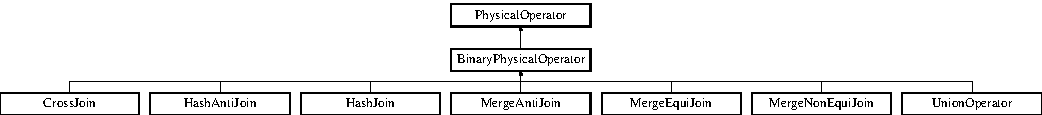
\includegraphics[height=1.538462cm]{class_binary_physical_operator}
\end{center}
\end{figure}
\subsection*{Public Member Functions}
\begin{DoxyCompactItemize}
\item 
virtual void \hyperlink{class_binary_physical_operator_a29ec622920006cb5428bf2c259918347}{accept} (\hyperlink{class_physical_operator_visitor}{Physical\+Operator\+Visitor} \&v)=0
\end{DoxyCompactItemize}
\subsection*{Public Attributes}
\begin{DoxyCompactItemize}
\item 
std\+::shared\+\_\+ptr$<$ \hyperlink{class_physical_operator}{Physical\+Operator} $>$ \hyperlink{class_binary_physical_operator_a60ea09dbc34f680f024a9946c3634cbd}{left\+Child}
\item 
std\+::shared\+\_\+ptr$<$ \hyperlink{class_physical_operator}{Physical\+Operator} $>$ \hyperlink{class_binary_physical_operator_a9247498cd4b4e35968e2aa78bac17016}{right\+Child}
\end{DoxyCompactItemize}


\subsection{Detailed Description}
Base class for operators with two inputs. 

\subsection{Member Function Documentation}
\hypertarget{class_binary_physical_operator_a29ec622920006cb5428bf2c259918347}{\index{Binary\+Physical\+Operator@{Binary\+Physical\+Operator}!accept@{accept}}
\index{accept@{accept}!Binary\+Physical\+Operator@{Binary\+Physical\+Operator}}
\subsubsection[{accept}]{\setlength{\rightskip}{0pt plus 5cm}virtual void Binary\+Physical\+Operator\+::accept (
\begin{DoxyParamCaption}
\item[{{\bf Physical\+Operator\+Visitor} \&}]{v}
\end{DoxyParamCaption}
)\hspace{0.3cm}{\ttfamily [pure virtual]}}}\label{class_binary_physical_operator_a29ec622920006cb5428bf2c259918347}
Method for calling visit\mbox{[}node\mbox{]} on given \hyperlink{class_physical_operator_visitor}{Physical\+Operator\+Visitor}. 
\begin{DoxyParams}{Parameters}
{\em v} & \hyperlink{class_physical_operator_visitor}{Physical\+Operator\+Visitor}, on which to call function. \\
\hline
\end{DoxyParams}


Implements \hyperlink{class_physical_operator_aec6926a904c71c0619d6e9e1457252cd}{Physical\+Operator}.



Implemented in \hyperlink{class_union_operator_a534cf044caa5074d4a493edff1209e16}{Union\+Operator}, \hyperlink{class_merge_anti_join_a15758e7f808703b243101faa382a0156}{Merge\+Anti\+Join}, \hyperlink{class_hash_anti_join_a8a629e5592d9a42ce155dd83f7f551d0}{Hash\+Anti\+Join}, \hyperlink{class_hash_join_a11dc03e38397ff42352772a3c759e145}{Hash\+Join}, \hyperlink{class_merge_equi_join_a0a88e744444a5a539d58aac25c609a9c}{Merge\+Equi\+Join}, \hyperlink{class_merge_non_equi_join_a117ec79e9941977b4f90c65bea5cea65}{Merge\+Non\+Equi\+Join}, and \hyperlink{class_cross_join_a92a1a35e3940c6c8bdaa6722d476c5db}{Cross\+Join}.



\subsection{Member Data Documentation}
\hypertarget{class_binary_physical_operator_a60ea09dbc34f680f024a9946c3634cbd}{\index{Binary\+Physical\+Operator@{Binary\+Physical\+Operator}!left\+Child@{left\+Child}}
\index{left\+Child@{left\+Child}!Binary\+Physical\+Operator@{Binary\+Physical\+Operator}}
\subsubsection[{left\+Child}]{\setlength{\rightskip}{0pt plus 5cm}std\+::shared\+\_\+ptr$<${\bf Physical\+Operator}$>$ Binary\+Physical\+Operator\+::left\+Child}}\label{class_binary_physical_operator_a60ea09dbc34f680f024a9946c3634cbd}
Stores left input operator. \hypertarget{class_binary_physical_operator_a9247498cd4b4e35968e2aa78bac17016}{\index{Binary\+Physical\+Operator@{Binary\+Physical\+Operator}!right\+Child@{right\+Child}}
\index{right\+Child@{right\+Child}!Binary\+Physical\+Operator@{Binary\+Physical\+Operator}}
\subsubsection[{right\+Child}]{\setlength{\rightskip}{0pt plus 5cm}std\+::shared\+\_\+ptr$<${\bf Physical\+Operator}$>$ Binary\+Physical\+Operator\+::right\+Child}}\label{class_binary_physical_operator_a9247498cd4b4e35968e2aa78bac17016}
Stores right input operator. 

The documentation for this class was generated from the following file\+:\begin{DoxyCompactItemize}
\item 
C\+:/\+Users/\+Marcel/\+Documents/\+Visual Studio 2012/\+Projects/\+Relational\+Query\+Evaluator/\+Relational\+Query\+Evaluator/Physical\+Operator.\+h\end{DoxyCompactItemize}

\hypertarget{class_bobox_plan_writing_physical_operator_visitor}{\section{Bobox\+Plan\+Writing\+Physical\+Operator\+Visitor Class Reference}
\label{class_bobox_plan_writing_physical_operator_visitor}\index{Bobox\+Plan\+Writing\+Physical\+Operator\+Visitor@{Bobox\+Plan\+Writing\+Physical\+Operator\+Visitor}}
}
Inheritance diagram for Bobox\+Plan\+Writing\+Physical\+Operator\+Visitor\+:\begin{figure}[H]
\begin{center}
\leavevmode
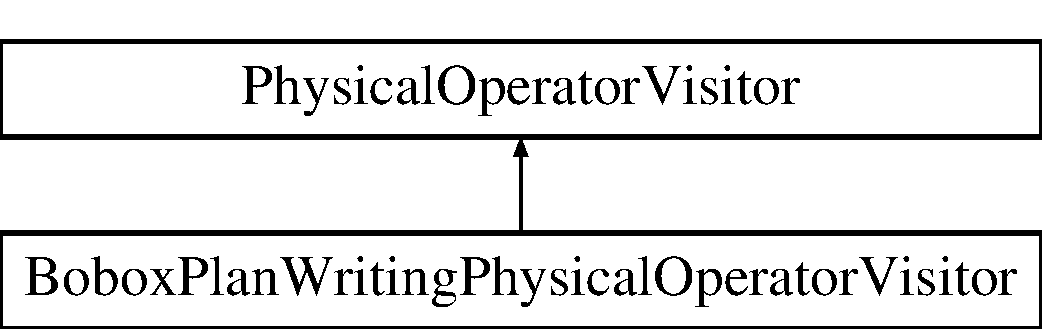
\includegraphics[height=2.000000cm]{class_bobox_plan_writing_physical_operator_visitor}
\end{center}
\end{figure}
\subsection*{Public Member Functions}
\begin{DoxyCompactItemize}
\item 
\hypertarget{class_bobox_plan_writing_physical_operator_visitor_a67767e3ad079b9fd8d431c230aed3f73}{std\+::string {\bfseries declaration} (const std\+::string \&type, const std\+::string \&input\+Columns, const std\+::string \&output\+Columns, const std\+::string \&name, const std\+::string \&construct\+Parameters)}\label{class_bobox_plan_writing_physical_operator_visitor_a67767e3ad079b9fd8d431c230aed3f73}

\item 
\hypertarget{class_bobox_plan_writing_physical_operator_visitor_a9dc928a4e3a478c260036bbc44daf302}{std\+::string {\bfseries connect} (const std\+::string \&from, const std\+::string \&to)}\label{class_bobox_plan_writing_physical_operator_visitor_a9dc928a4e3a478c260036bbc44daf302}

\item 
\hypertarget{class_bobox_plan_writing_physical_operator_visitor_ad19fe61538f80b821617614a31e30cb2}{std\+::string {\bfseries write\+Plan} (std\+::shared\+\_\+ptr$<$ \hyperlink{class_physical_operator}{Physical\+Operator} $>$ \&plan)}\label{class_bobox_plan_writing_physical_operator_visitor_ad19fe61538f80b821617614a31e30cb2}

\item 
\hypertarget{class_bobox_plan_writing_physical_operator_visitor_a09857e8ac9d485ca1a749e06fd447a4a}{std\+::string {\bfseries get\+Column\+Type\+Output} (const std\+::map$<$ int, \hyperlink{class_column_info}{Column\+Info} $>$ \&columns)}\label{class_bobox_plan_writing_physical_operator_visitor_a09857e8ac9d485ca1a749e06fd447a4a}

\item 
\hypertarget{class_bobox_plan_writing_physical_operator_visitor_ab10127e63906b7eb061f703cd7bb9252}{std\+::string {\bfseries get\+Column\+Name\+Output} (const std\+::map$<$ int, \hyperlink{class_column_info}{Column\+Info} $>$ \&columns)}\label{class_bobox_plan_writing_physical_operator_visitor_ab10127e63906b7eb061f703cd7bb9252}

\item 
\hypertarget{class_bobox_plan_writing_physical_operator_visitor_aa41f0bb800a4584a5d2baa160f3b064a}{std\+::string {\bfseries get\+Id} ()}\label{class_bobox_plan_writing_physical_operator_visitor_aa41f0bb800a4584a5d2baa160f3b064a}

\item 
\hypertarget{class_bobox_plan_writing_physical_operator_visitor_a809cf16afde7b5714466438602925355}{void {\bfseries convert\+Columns} (const std\+::map$<$ int, \hyperlink{class_column_info}{Column\+Info} $>$ \&columns, std\+::map$<$ int, int $>$ \&result)}\label{class_bobox_plan_writing_physical_operator_visitor_a809cf16afde7b5714466438602925355}

\item 
\hypertarget{class_bobox_plan_writing_physical_operator_visitor_a3d0b2c26562a904deac5d003eee02faf}{void {\bfseries write\+Nullary\+Operator} (const std\+::string \&type, const std\+::map$<$ int, \hyperlink{class_column_info}{Column\+Info} $>$ \&columns, const std\+::string \&costructor\+Parameters)}\label{class_bobox_plan_writing_physical_operator_visitor_a3d0b2c26562a904deac5d003eee02faf}

\item 
\hypertarget{class_bobox_plan_writing_physical_operator_visitor_aacdb98a45fe5a45d5f86898e4b6d4ff1}{void {\bfseries write\+Unary\+Operator} (const std\+::string \&type, \hyperlink{class_unary_physical_operator}{Unary\+Physical\+Operator} $\ast$node, const std\+::string \&costructor\+Parameters)}\label{class_bobox_plan_writing_physical_operator_visitor_aacdb98a45fe5a45d5f86898e4b6d4ff1}

\item 
\hypertarget{class_bobox_plan_writing_physical_operator_visitor_a2a3636390a5c12828b2814ac96a46410}{void {\bfseries write\+Binary\+Operator} (const std\+::string \&type, \hyperlink{class_binary_physical_operator}{Binary\+Physical\+Operator} $\ast$node, const std\+::string \&costructor\+Parameters)}\label{class_bobox_plan_writing_physical_operator_visitor_a2a3636390a5c12828b2814ac96a46410}

\item 
\hypertarget{class_bobox_plan_writing_physical_operator_visitor_a96eb34b06365296896e890123abdfa01}{std\+::string {\bfseries write\+Group\+Parameters} (const std\+::map$<$ int, \hyperlink{class_column_info}{Column\+Info} $>$ \&output\+Columns, const std\+::map$<$ int, \hyperlink{class_column_info}{Column\+Info} $>$ \&input\+Columns, const std\+::vector$<$ \hyperlink{class_group_column}{Group\+Column} $>$ \&group\+Columns, const std\+::vector$<$ \hyperlink{class_agregate_function}{Agregate\+Function} $>$ \&agregate\+Functions)}\label{class_bobox_plan_writing_physical_operator_visitor_a96eb34b06365296896e890123abdfa01}

\item 
\hypertarget{class_bobox_plan_writing_physical_operator_visitor_a1a836021544f1e6cd117620b888819ba}{std\+::string {\bfseries write\+Join\+Parameters} (\hyperlink{class_binary_physical_operator}{Binary\+Physical\+Operator} $\ast$node)}\label{class_bobox_plan_writing_physical_operator_visitor_a1a836021544f1e6cd117620b888819ba}

\item 
\hypertarget{class_bobox_plan_writing_physical_operator_visitor_a03f4fd96dbe1a60b5e562a3e200d1263}{std\+::string {\bfseries write\+Equi\+Join\+Parameters} (const std\+::vector$<$ \hyperlink{class_column_identifier}{Column\+Identifier} $>$ \&left, const std\+::vector$<$ \hyperlink{class_column_identifier}{Column\+Identifier} $>$ \&right, \hyperlink{class_binary_physical_operator}{Binary\+Physical\+Operator} $\ast$node)}\label{class_bobox_plan_writing_physical_operator_visitor_a03f4fd96dbe1a60b5e562a3e200d1263}

\item 
\hypertarget{class_bobox_plan_writing_physical_operator_visitor_a30e0f62016ad2037261b8daa69752d5f}{std\+::string {\bfseries write\+Merge\+Equi\+Join\+Parameters} (const std\+::vector$<$ \hyperlink{class_sort_parameter}{Sort\+Parameter} $>$ \&left, const std\+::vector$<$ \hyperlink{class_sort_parameter}{Sort\+Parameter} $>$ \&right, \hyperlink{class_binary_physical_operator}{Binary\+Physical\+Operator} $\ast$node)}\label{class_bobox_plan_writing_physical_operator_visitor_a30e0f62016ad2037261b8daa69752d5f}

\item 
\hypertarget{class_bobox_plan_writing_physical_operator_visitor_a443e89add4155e51b2d7d1973afb3af5}{void {\bfseries visit\+Filter} (\hyperlink{class_filter}{Filter} $\ast$node)}\label{class_bobox_plan_writing_physical_operator_visitor_a443e89add4155e51b2d7d1973afb3af5}

\item 
\hypertarget{class_bobox_plan_writing_physical_operator_visitor_a041f79a1705915af0d45e623ad7a18ac}{void {\bfseries visit\+Filter\+Keeping\+Order} (\hyperlink{class_filter_keeping_order}{Filter\+Keeping\+Order} $\ast$node)}\label{class_bobox_plan_writing_physical_operator_visitor_a041f79a1705915af0d45e623ad7a18ac}

\item 
\hypertarget{class_bobox_plan_writing_physical_operator_visitor_ac482fb6eae4e0bcb957bad6c572a2c03}{void {\bfseries visit\+Sort\+Operator} (\hyperlink{class_sort_operator}{Sort\+Operator} $\ast$node)}\label{class_bobox_plan_writing_physical_operator_visitor_ac482fb6eae4e0bcb957bad6c572a2c03}

\item 
\hypertarget{class_bobox_plan_writing_physical_operator_visitor_ac66108bf441456b57aded81ac17b111b}{void {\bfseries visit\+Merge\+Equi\+Join} (\hyperlink{class_merge_equi_join}{Merge\+Equi\+Join} $\ast$node)}\label{class_bobox_plan_writing_physical_operator_visitor_ac66108bf441456b57aded81ac17b111b}

\item 
\hypertarget{class_bobox_plan_writing_physical_operator_visitor_a75a1a20aecd434d712dff1867bf5ec37}{void {\bfseries visit\+Merge\+Non\+Equi\+Join} (\hyperlink{class_merge_non_equi_join}{Merge\+Non\+Equi\+Join} $\ast$node)}\label{class_bobox_plan_writing_physical_operator_visitor_a75a1a20aecd434d712dff1867bf5ec37}

\item 
\hypertarget{class_bobox_plan_writing_physical_operator_visitor_a882ad63c59098b1bca68fca5d36b8871}{void {\bfseries visit\+Cross\+Join} (\hyperlink{class_cross_join}{Cross\+Join} $\ast$node)}\label{class_bobox_plan_writing_physical_operator_visitor_a882ad63c59098b1bca68fca5d36b8871}

\item 
\hypertarget{class_bobox_plan_writing_physical_operator_visitor_a5616d43abbe0666c854342af2d3aec94}{void {\bfseries visit\+Hash\+Join} (\hyperlink{class_hash_join}{Hash\+Join} $\ast$node)}\label{class_bobox_plan_writing_physical_operator_visitor_a5616d43abbe0666c854342af2d3aec94}

\item 
\hypertarget{class_bobox_plan_writing_physical_operator_visitor_a01ed46af47fc5c7fb7af2b6b5b2483ba}{void {\bfseries visit\+Hash\+Anti\+Join} (\hyperlink{class_hash_anti_join}{Hash\+Anti\+Join} $\ast$node)}\label{class_bobox_plan_writing_physical_operator_visitor_a01ed46af47fc5c7fb7af2b6b5b2483ba}

\item 
\hypertarget{class_bobox_plan_writing_physical_operator_visitor_a0346b44be20be9fb68d95029908808f6}{void {\bfseries visit\+Merge\+Anti\+Join} (\hyperlink{class_merge_anti_join}{Merge\+Anti\+Join} $\ast$node)}\label{class_bobox_plan_writing_physical_operator_visitor_a0346b44be20be9fb68d95029908808f6}

\item 
\hypertarget{class_bobox_plan_writing_physical_operator_visitor_a87c2ddbe5d05b7dcc30c9d61d540d1f5}{void {\bfseries visit\+Union\+Operator} (\hyperlink{class_union_operator}{Union\+Operator} $\ast$node)}\label{class_bobox_plan_writing_physical_operator_visitor_a87c2ddbe5d05b7dcc30c9d61d540d1f5}

\item 
\hypertarget{class_bobox_plan_writing_physical_operator_visitor_a1e114b9a6e5bf08a691a9197f03efe9d}{void {\bfseries visit\+Hash\+Group} (\hyperlink{class_hash_group}{Hash\+Group} $\ast$node)}\label{class_bobox_plan_writing_physical_operator_visitor_a1e114b9a6e5bf08a691a9197f03efe9d}

\item 
\hypertarget{class_bobox_plan_writing_physical_operator_visitor_a78d8526758ffeb3b335b8fc4a8a2defb}{void {\bfseries visit\+Sorted\+Group} (\hyperlink{class_sorted_group}{Sorted\+Group} $\ast$node)}\label{class_bobox_plan_writing_physical_operator_visitor_a78d8526758ffeb3b335b8fc4a8a2defb}

\item 
\hypertarget{class_bobox_plan_writing_physical_operator_visitor_afe09e3f584a43ff5e06947918cf16a46}{void {\bfseries visit\+Columns\+Operations\+Operator} (\hyperlink{class_columns_operations_operator}{Columns\+Operations\+Operator} $\ast$node)}\label{class_bobox_plan_writing_physical_operator_visitor_afe09e3f584a43ff5e06947918cf16a46}

\item 
\hypertarget{class_bobox_plan_writing_physical_operator_visitor_a09cbea340b85723f8e66e50b466d6e68}{void {\bfseries visit\+Scan\+And\+Sort\+By\+Index} (\hyperlink{class_scan_and_sort_by_index}{Scan\+And\+Sort\+By\+Index} $\ast$node)}\label{class_bobox_plan_writing_physical_operator_visitor_a09cbea340b85723f8e66e50b466d6e68}

\item 
\hypertarget{class_bobox_plan_writing_physical_operator_visitor_aa8d995c39b2364625c1c10b6d7636b23}{void {\bfseries visit\+Table\+Scan} (\hyperlink{class_table_scan}{Table\+Scan} $\ast$node)}\label{class_bobox_plan_writing_physical_operator_visitor_aa8d995c39b2364625c1c10b6d7636b23}

\item 
\hypertarget{class_bobox_plan_writing_physical_operator_visitor_ae042371767ff5d9296468da8037efa0f}{void {\bfseries visit\+Index\+Scan} (\hyperlink{class_index_scan}{Index\+Scan} $\ast$node)}\label{class_bobox_plan_writing_physical_operator_visitor_ae042371767ff5d9296468da8037efa0f}

\end{DoxyCompactItemize}


The documentation for this class was generated from the following files\+:\begin{DoxyCompactItemize}
\item 
C\+:/\+Users/\+Marcel/\+Documents/\+Visual Studio 2012/\+Projects/\+Relational\+Query\+Evaluator/\+Relational\+Query\+Evaluator/Physical\+Operator\+Visitor.\+h\item 
C\+:/\+Users/\+Marcel/\+Documents/\+Visual Studio 2012/\+Projects/\+Relational\+Query\+Evaluator/\+Relational\+Query\+Evaluator/Bobox\+Output.\+cpp\end{DoxyCompactItemize}

\hypertarget{class_bobox_writing_expression_visitor}{\section{Bobox\+Writing\+Expression\+Visitor Class Reference}
\label{class_bobox_writing_expression_visitor}\index{Bobox\+Writing\+Expression\+Visitor@{Bobox\+Writing\+Expression\+Visitor}}
}


{\ttfamily \#include $<$Expression\+Visitors.\+h$>$}

Inheritance diagram for Bobox\+Writing\+Expression\+Visitor\+:\begin{figure}[H]
\begin{center}
\leavevmode
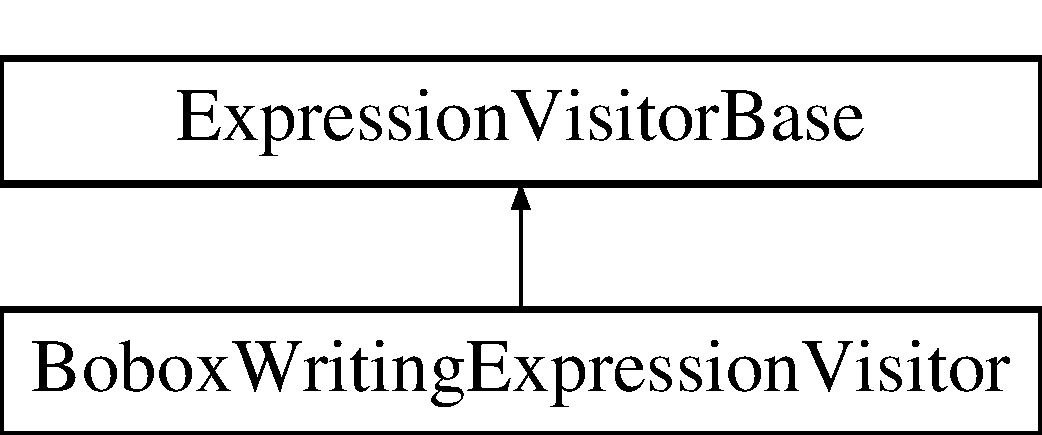
\includegraphics[height=2.000000cm]{class_bobox_writing_expression_visitor}
\end{center}
\end{figure}
\subsection*{Public Member Functions}
\begin{DoxyCompactItemize}
\item 
\hyperlink{class_bobox_writing_expression_visitor_a977d27ae446d613bc90fb6e29165504b}{Bobox\+Writing\+Expression\+Visitor} (std\+::map$<$ int, int $>$ \&\hyperlink{class_bobox_writing_expression_visitor_a6e0d9ba1a06fd32c8d71dd8e1c068c56}{cols})
\item 
void \hyperlink{class_bobox_writing_expression_visitor_abf4dc22d06dd87f35f577db194b69a71}{visit\+Unary\+Expression} (\hyperlink{class_unary_expression}{Unary\+Expression} $\ast$expression)
\item 
void \hyperlink{class_bobox_writing_expression_visitor_a4e7d193e7b5d361c67a0ee0b82628120}{visit\+Binary\+Expression} (\hyperlink{class_binary_expression}{Binary\+Expression} $\ast$expression)
\item 
void \hyperlink{class_bobox_writing_expression_visitor_ac66d4abc015382d70392acc6593196c3}{visit\+Nnary\+Expression} (\hyperlink{class_nnary_expression}{Nnary\+Expression} $\ast$expression)
\item 
void \hyperlink{class_bobox_writing_expression_visitor_aa51161e2a5c08a3f5ca37901fbcc572f}{visit\+Constant} (\hyperlink{class_constant}{Constant} $\ast$expression)
\item 
void \hyperlink{class_bobox_writing_expression_visitor_a2547b638ff123190d33492ed3ce410ea}{visit\+Column} (\hyperlink{class_column}{Column} $\ast$expression)
\item 
void \hyperlink{class_bobox_writing_expression_visitor_a12180fc75d31108cf8c542513e0f1db5}{visit\+Grouped\+Expression} (\hyperlink{class_grouped_expression}{Grouped\+Expression} $\ast$expression)
\end{DoxyCompactItemize}
\subsection*{Public Attributes}
\begin{DoxyCompactItemize}
\item 
std\+::string \hyperlink{class_bobox_writing_expression_visitor_a222842d9f796beebabc13691b107e5ad}{result}
\item 
std\+::map$<$ int, int $>$ $\ast$ \hyperlink{class_bobox_writing_expression_visitor_a6e0d9ba1a06fd32c8d71dd8e1c068c56}{cols}
\end{DoxyCompactItemize}


\subsection{Detailed Description}
Visitor writes expression in infix for bobox output. 

\subsection{Constructor \& Destructor Documentation}
\hypertarget{class_bobox_writing_expression_visitor_a977d27ae446d613bc90fb6e29165504b}{\index{Bobox\+Writing\+Expression\+Visitor@{Bobox\+Writing\+Expression\+Visitor}!Bobox\+Writing\+Expression\+Visitor@{Bobox\+Writing\+Expression\+Visitor}}
\index{Bobox\+Writing\+Expression\+Visitor@{Bobox\+Writing\+Expression\+Visitor}!Bobox\+Writing\+Expression\+Visitor@{Bobox\+Writing\+Expression\+Visitor}}
\subsubsection[{Bobox\+Writing\+Expression\+Visitor}]{\setlength{\rightskip}{0pt plus 5cm}Bobox\+Writing\+Expression\+Visitor\+::\+Bobox\+Writing\+Expression\+Visitor (
\begin{DoxyParamCaption}
\item[{std\+::map$<$ int, int $>$ \&}]{cols}
\end{DoxyParamCaption}
)}}\label{class_bobox_writing_expression_visitor_a977d27ae446d613bc90fb6e29165504b}
Creates new instance of \hyperlink{class_bobox_writing_expression_visitor}{Bobox\+Writing\+Expression\+Visitor}. 
\begin{DoxyParams}{Parameters}
{\em cols} & -\/ structure mapping column unique identifier to number of column in processed bobox operator \\
\hline
\end{DoxyParams}


\subsection{Member Function Documentation}
\hypertarget{class_bobox_writing_expression_visitor_a4e7d193e7b5d361c67a0ee0b82628120}{\index{Bobox\+Writing\+Expression\+Visitor@{Bobox\+Writing\+Expression\+Visitor}!visit\+Binary\+Expression@{visit\+Binary\+Expression}}
\index{visit\+Binary\+Expression@{visit\+Binary\+Expression}!Bobox\+Writing\+Expression\+Visitor@{Bobox\+Writing\+Expression\+Visitor}}
\subsubsection[{visit\+Binary\+Expression}]{\setlength{\rightskip}{0pt plus 5cm}void Bobox\+Writing\+Expression\+Visitor\+::visit\+Binary\+Expression (
\begin{DoxyParamCaption}
\item[{{\bf Binary\+Expression} $\ast$}]{expression}
\end{DoxyParamCaption}
)\hspace{0.3cm}{\ttfamily [virtual]}}}\label{class_bobox_writing_expression_visitor_a4e7d193e7b5d361c67a0ee0b82628120}
Visits \hyperlink{class_binary_expression}{Binary\+Expression} element. 
\begin{DoxyParams}{Parameters}
{\em expression} & visited \hyperlink{class_binary_expression}{Binary\+Expression}. \\
\hline
\end{DoxyParams}


Reimplemented from \hyperlink{class_expression_visitor_base_aebbbbe9a1cecabe4c4804bf1ef82a9f9}{Expression\+Visitor\+Base}.

\hypertarget{class_bobox_writing_expression_visitor_a2547b638ff123190d33492ed3ce410ea}{\index{Bobox\+Writing\+Expression\+Visitor@{Bobox\+Writing\+Expression\+Visitor}!visit\+Column@{visit\+Column}}
\index{visit\+Column@{visit\+Column}!Bobox\+Writing\+Expression\+Visitor@{Bobox\+Writing\+Expression\+Visitor}}
\subsubsection[{visit\+Column}]{\setlength{\rightskip}{0pt plus 5cm}void Bobox\+Writing\+Expression\+Visitor\+::visit\+Column (
\begin{DoxyParamCaption}
\item[{{\bf Column} $\ast$}]{expression}
\end{DoxyParamCaption}
)\hspace{0.3cm}{\ttfamily [virtual]}}}\label{class_bobox_writing_expression_visitor_a2547b638ff123190d33492ed3ce410ea}
Visits \hyperlink{class_column}{Column} element. 
\begin{DoxyParams}{Parameters}
{\em expression} & visited \hyperlink{class_column}{Column}. \\
\hline
\end{DoxyParams}


Reimplemented from \hyperlink{class_expression_visitor_base_a1ac638b82248ff9e1582dbf520dc6ae4}{Expression\+Visitor\+Base}.

\hypertarget{class_bobox_writing_expression_visitor_aa51161e2a5c08a3f5ca37901fbcc572f}{\index{Bobox\+Writing\+Expression\+Visitor@{Bobox\+Writing\+Expression\+Visitor}!visit\+Constant@{visit\+Constant}}
\index{visit\+Constant@{visit\+Constant}!Bobox\+Writing\+Expression\+Visitor@{Bobox\+Writing\+Expression\+Visitor}}
\subsubsection[{visit\+Constant}]{\setlength{\rightskip}{0pt plus 5cm}void Bobox\+Writing\+Expression\+Visitor\+::visit\+Constant (
\begin{DoxyParamCaption}
\item[{{\bf Constant} $\ast$}]{expression}
\end{DoxyParamCaption}
)\hspace{0.3cm}{\ttfamily [virtual]}}}\label{class_bobox_writing_expression_visitor_aa51161e2a5c08a3f5ca37901fbcc572f}
Visits \hyperlink{class_constant}{Constant} element. 
\begin{DoxyParams}{Parameters}
{\em expression} & visited \hyperlink{class_constant}{Constant}. \\
\hline
\end{DoxyParams}


Reimplemented from \hyperlink{class_expression_visitor_base_a64921e6a6a4945faf693e9ef8d6310a4}{Expression\+Visitor\+Base}.

\hypertarget{class_bobox_writing_expression_visitor_a12180fc75d31108cf8c542513e0f1db5}{\index{Bobox\+Writing\+Expression\+Visitor@{Bobox\+Writing\+Expression\+Visitor}!visit\+Grouped\+Expression@{visit\+Grouped\+Expression}}
\index{visit\+Grouped\+Expression@{visit\+Grouped\+Expression}!Bobox\+Writing\+Expression\+Visitor@{Bobox\+Writing\+Expression\+Visitor}}
\subsubsection[{visit\+Grouped\+Expression}]{\setlength{\rightskip}{0pt plus 5cm}void Bobox\+Writing\+Expression\+Visitor\+::visit\+Grouped\+Expression (
\begin{DoxyParamCaption}
\item[{{\bf Grouped\+Expression} $\ast$}]{expression}
\end{DoxyParamCaption}
)\hspace{0.3cm}{\ttfamily [virtual]}}}\label{class_bobox_writing_expression_visitor_a12180fc75d31108cf8c542513e0f1db5}
Visits \hyperlink{class_grouped_expression}{Grouped\+Expression} element. 
\begin{DoxyParams}{Parameters}
{\em expression} & visited \hyperlink{class_grouped_expression}{Grouped\+Expression}. \\
\hline
\end{DoxyParams}


Reimplemented from \hyperlink{class_expression_visitor_base_aec22a7bb476fc79e7997d188423514c0}{Expression\+Visitor\+Base}.

\hypertarget{class_bobox_writing_expression_visitor_ac66d4abc015382d70392acc6593196c3}{\index{Bobox\+Writing\+Expression\+Visitor@{Bobox\+Writing\+Expression\+Visitor}!visit\+Nnary\+Expression@{visit\+Nnary\+Expression}}
\index{visit\+Nnary\+Expression@{visit\+Nnary\+Expression}!Bobox\+Writing\+Expression\+Visitor@{Bobox\+Writing\+Expression\+Visitor}}
\subsubsection[{visit\+Nnary\+Expression}]{\setlength{\rightskip}{0pt plus 5cm}void Bobox\+Writing\+Expression\+Visitor\+::visit\+Nnary\+Expression (
\begin{DoxyParamCaption}
\item[{{\bf Nnary\+Expression} $\ast$}]{expression}
\end{DoxyParamCaption}
)\hspace{0.3cm}{\ttfamily [virtual]}}}\label{class_bobox_writing_expression_visitor_ac66d4abc015382d70392acc6593196c3}
Visits \hyperlink{class_nnary_expression}{Nnary\+Expression} element. 
\begin{DoxyParams}{Parameters}
{\em expression} & visited \hyperlink{class_nnary_expression}{Nnary\+Expression}. \\
\hline
\end{DoxyParams}


Reimplemented from \hyperlink{class_expression_visitor_base_a010c5ba36b255c8576a2b36aaf9692d8}{Expression\+Visitor\+Base}.

\hypertarget{class_bobox_writing_expression_visitor_abf4dc22d06dd87f35f577db194b69a71}{\index{Bobox\+Writing\+Expression\+Visitor@{Bobox\+Writing\+Expression\+Visitor}!visit\+Unary\+Expression@{visit\+Unary\+Expression}}
\index{visit\+Unary\+Expression@{visit\+Unary\+Expression}!Bobox\+Writing\+Expression\+Visitor@{Bobox\+Writing\+Expression\+Visitor}}
\subsubsection[{visit\+Unary\+Expression}]{\setlength{\rightskip}{0pt plus 5cm}void Bobox\+Writing\+Expression\+Visitor\+::visit\+Unary\+Expression (
\begin{DoxyParamCaption}
\item[{{\bf Unary\+Expression} $\ast$}]{expression}
\end{DoxyParamCaption}
)\hspace{0.3cm}{\ttfamily [virtual]}}}\label{class_bobox_writing_expression_visitor_abf4dc22d06dd87f35f577db194b69a71}
Visits \hyperlink{class_unary_expression}{Unary\+Expression} element. 
\begin{DoxyParams}{Parameters}
{\em expression} & visited \hyperlink{class_unary_expression}{Unary\+Expression}. \\
\hline
\end{DoxyParams}


Reimplemented from \hyperlink{class_expression_visitor_base_a9750397f5588263509a28ca9f17e8bc4}{Expression\+Visitor\+Base}.



\subsection{Member Data Documentation}
\hypertarget{class_bobox_writing_expression_visitor_a6e0d9ba1a06fd32c8d71dd8e1c068c56}{\index{Bobox\+Writing\+Expression\+Visitor@{Bobox\+Writing\+Expression\+Visitor}!cols@{cols}}
\index{cols@{cols}!Bobox\+Writing\+Expression\+Visitor@{Bobox\+Writing\+Expression\+Visitor}}
\subsubsection[{cols}]{\setlength{\rightskip}{0pt plus 5cm}std\+::map$<$int, int$>$$\ast$ Bobox\+Writing\+Expression\+Visitor\+::cols}}\label{class_bobox_writing_expression_visitor_a6e0d9ba1a06fd32c8d71dd8e1c068c56}
Structure mapping column unique identifier to number of column in processed bobox operator. \hypertarget{class_bobox_writing_expression_visitor_a222842d9f796beebabc13691b107e5ad}{\index{Bobox\+Writing\+Expression\+Visitor@{Bobox\+Writing\+Expression\+Visitor}!result@{result}}
\index{result@{result}!Bobox\+Writing\+Expression\+Visitor@{Bobox\+Writing\+Expression\+Visitor}}
\subsubsection[{result}]{\setlength{\rightskip}{0pt plus 5cm}std\+::string Bobox\+Writing\+Expression\+Visitor\+::result}}\label{class_bobox_writing_expression_visitor_a222842d9f796beebabc13691b107e5ad}
Stores tree infix representation. 

The documentation for this class was generated from the following files\+:\begin{DoxyCompactItemize}
\item 
C\+:/\+Users/\+Marcel/\+Documents/\+Visual Studio 2012/\+Projects/\+Relational\+Query\+Evaluator/\+Relational\+Query\+Evaluator/Expression\+Visitors.\+h\item 
C\+:/\+Users/\+Marcel/\+Documents/\+Visual Studio 2012/\+Projects/\+Relational\+Query\+Evaluator/\+Relational\+Query\+Evaluator/Bobox\+Output.\+cpp\end{DoxyCompactItemize}

\hypertarget{class_cloning_expression_visitor}{\section{Cloning\+Expression\+Visitor Class Reference}
\label{class_cloning_expression_visitor}\index{Cloning\+Expression\+Visitor@{Cloning\+Expression\+Visitor}}
}
Inheritance diagram for Cloning\+Expression\+Visitor\+:\begin{figure}[H]
\begin{center}
\leavevmode
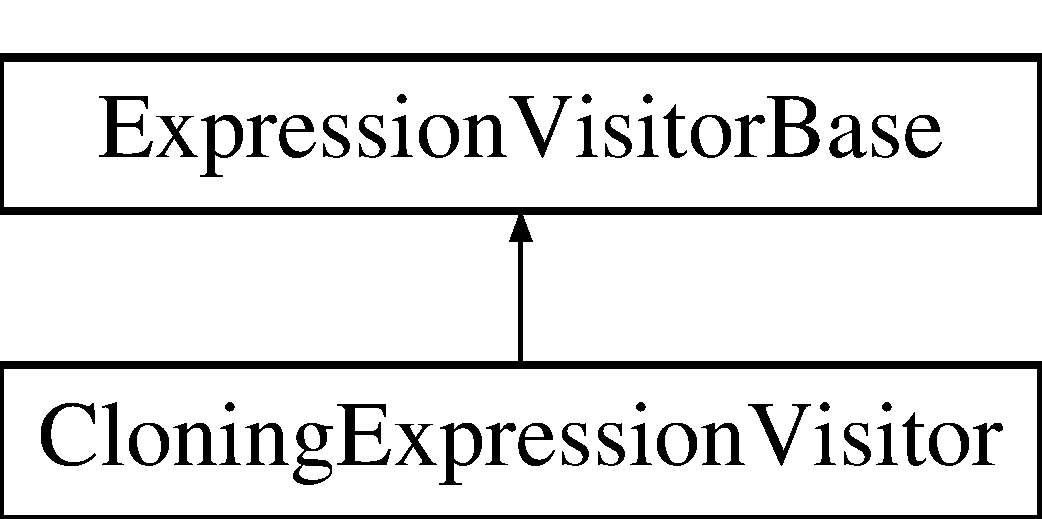
\includegraphics[height=2.000000cm]{class_cloning_expression_visitor}
\end{center}
\end{figure}
\subsection*{Public Member Functions}
\begin{DoxyCompactItemize}
\item 
void \hyperlink{class_cloning_expression_visitor_a5eef4362b38190ddadda4c3a6c530475}{visit\+Unary\+Expression} (\hyperlink{class_unary_expression}{Unary\+Expression} $\ast$expression)
\item 
void \hyperlink{class_cloning_expression_visitor_a6a7ba77a1e2b18837d5968d8c9c6e1bc}{visit\+Binary\+Expression} (\hyperlink{class_binary_expression}{Binary\+Expression} $\ast$expression)
\item 
void \hyperlink{class_cloning_expression_visitor_ac09c5ce926f720992e6799b39625fbc2}{visit\+Nnary\+Expression} (\hyperlink{class_nnary_expression}{Nnary\+Expression} $\ast$expression)
\item 
void \hyperlink{class_cloning_expression_visitor_af88937b26b66507f653a0370f51e2fa1}{visit\+Constant} (\hyperlink{class_constant}{Constant} $\ast$expression)
\item 
void \hyperlink{class_cloning_expression_visitor_aae3630ba345d058f2b1be2ae6c83340c}{visit\+Column} (\hyperlink{class_column}{Column} $\ast$expression)
\item 
void \hyperlink{class_cloning_expression_visitor_af5bd6b26028188a7a582a2236342e339}{visit\+Grouped\+Expression} (\hyperlink{class_grouped_expression}{Grouped\+Expression} $\ast$expression)
\end{DoxyCompactItemize}
\subsection*{Public Attributes}
\begin{DoxyCompactItemize}
\item 
\hypertarget{class_cloning_expression_visitor_aa23b5af5203ff9b14ee556a527173ad3}{std\+::shared\+\_\+ptr$<$ \hyperlink{class_expression}{Expression} $>$ {\bfseries result}}\label{class_cloning_expression_visitor_aa23b5af5203ff9b14ee556a527173ad3}

\end{DoxyCompactItemize}


\subsection{Member Function Documentation}
\hypertarget{class_cloning_expression_visitor_a6a7ba77a1e2b18837d5968d8c9c6e1bc}{\index{Cloning\+Expression\+Visitor@{Cloning\+Expression\+Visitor}!visit\+Binary\+Expression@{visit\+Binary\+Expression}}
\index{visit\+Binary\+Expression@{visit\+Binary\+Expression}!Cloning\+Expression\+Visitor@{Cloning\+Expression\+Visitor}}
\subsubsection[{visit\+Binary\+Expression}]{\setlength{\rightskip}{0pt plus 5cm}void Cloning\+Expression\+Visitor\+::visit\+Binary\+Expression (
\begin{DoxyParamCaption}
\item[{{\bf Binary\+Expression} $\ast$}]{expression}
\end{DoxyParamCaption}
)\hspace{0.3cm}{\ttfamily [virtual]}}}\label{class_cloning_expression_visitor_a6a7ba77a1e2b18837d5968d8c9c6e1bc}
Visits \hyperlink{class_binary_expression}{Binary\+Expression} element. 
\begin{DoxyParams}{Parameters}
{\em expression} & visited \hyperlink{class_binary_expression}{Binary\+Expression}. \\
\hline
\end{DoxyParams}


Reimplemented from \hyperlink{class_expression_visitor_base_aebbbbe9a1cecabe4c4804bf1ef82a9f9}{Expression\+Visitor\+Base}.

\hypertarget{class_cloning_expression_visitor_aae3630ba345d058f2b1be2ae6c83340c}{\index{Cloning\+Expression\+Visitor@{Cloning\+Expression\+Visitor}!visit\+Column@{visit\+Column}}
\index{visit\+Column@{visit\+Column}!Cloning\+Expression\+Visitor@{Cloning\+Expression\+Visitor}}
\subsubsection[{visit\+Column}]{\setlength{\rightskip}{0pt plus 5cm}void Cloning\+Expression\+Visitor\+::visit\+Column (
\begin{DoxyParamCaption}
\item[{{\bf Column} $\ast$}]{expression}
\end{DoxyParamCaption}
)\hspace{0.3cm}{\ttfamily [virtual]}}}\label{class_cloning_expression_visitor_aae3630ba345d058f2b1be2ae6c83340c}
Visits \hyperlink{class_column}{Column} element. 
\begin{DoxyParams}{Parameters}
{\em expression} & visited \hyperlink{class_column}{Column}. \\
\hline
\end{DoxyParams}


Reimplemented from \hyperlink{class_expression_visitor_base_a1ac638b82248ff9e1582dbf520dc6ae4}{Expression\+Visitor\+Base}.

\hypertarget{class_cloning_expression_visitor_af88937b26b66507f653a0370f51e2fa1}{\index{Cloning\+Expression\+Visitor@{Cloning\+Expression\+Visitor}!visit\+Constant@{visit\+Constant}}
\index{visit\+Constant@{visit\+Constant}!Cloning\+Expression\+Visitor@{Cloning\+Expression\+Visitor}}
\subsubsection[{visit\+Constant}]{\setlength{\rightskip}{0pt plus 5cm}void Cloning\+Expression\+Visitor\+::visit\+Constant (
\begin{DoxyParamCaption}
\item[{{\bf Constant} $\ast$}]{expression}
\end{DoxyParamCaption}
)\hspace{0.3cm}{\ttfamily [virtual]}}}\label{class_cloning_expression_visitor_af88937b26b66507f653a0370f51e2fa1}
Visits \hyperlink{class_constant}{Constant} element. 
\begin{DoxyParams}{Parameters}
{\em expression} & visited \hyperlink{class_constant}{Constant}. \\
\hline
\end{DoxyParams}


Reimplemented from \hyperlink{class_expression_visitor_base_a64921e6a6a4945faf693e9ef8d6310a4}{Expression\+Visitor\+Base}.

\hypertarget{class_cloning_expression_visitor_af5bd6b26028188a7a582a2236342e339}{\index{Cloning\+Expression\+Visitor@{Cloning\+Expression\+Visitor}!visit\+Grouped\+Expression@{visit\+Grouped\+Expression}}
\index{visit\+Grouped\+Expression@{visit\+Grouped\+Expression}!Cloning\+Expression\+Visitor@{Cloning\+Expression\+Visitor}}
\subsubsection[{visit\+Grouped\+Expression}]{\setlength{\rightskip}{0pt plus 5cm}void Cloning\+Expression\+Visitor\+::visit\+Grouped\+Expression (
\begin{DoxyParamCaption}
\item[{{\bf Grouped\+Expression} $\ast$}]{expression}
\end{DoxyParamCaption}
)\hspace{0.3cm}{\ttfamily [virtual]}}}\label{class_cloning_expression_visitor_af5bd6b26028188a7a582a2236342e339}
Visits \hyperlink{class_grouped_expression}{Grouped\+Expression} element. 
\begin{DoxyParams}{Parameters}
{\em expression} & visited \hyperlink{class_grouped_expression}{Grouped\+Expression}. \\
\hline
\end{DoxyParams}


Reimplemented from \hyperlink{class_expression_visitor_base_aec22a7bb476fc79e7997d188423514c0}{Expression\+Visitor\+Base}.

\hypertarget{class_cloning_expression_visitor_ac09c5ce926f720992e6799b39625fbc2}{\index{Cloning\+Expression\+Visitor@{Cloning\+Expression\+Visitor}!visit\+Nnary\+Expression@{visit\+Nnary\+Expression}}
\index{visit\+Nnary\+Expression@{visit\+Nnary\+Expression}!Cloning\+Expression\+Visitor@{Cloning\+Expression\+Visitor}}
\subsubsection[{visit\+Nnary\+Expression}]{\setlength{\rightskip}{0pt plus 5cm}void Cloning\+Expression\+Visitor\+::visit\+Nnary\+Expression (
\begin{DoxyParamCaption}
\item[{{\bf Nnary\+Expression} $\ast$}]{expression}
\end{DoxyParamCaption}
)\hspace{0.3cm}{\ttfamily [virtual]}}}\label{class_cloning_expression_visitor_ac09c5ce926f720992e6799b39625fbc2}
Visits \hyperlink{class_nnary_expression}{Nnary\+Expression} element. 
\begin{DoxyParams}{Parameters}
{\em expression} & visited \hyperlink{class_nnary_expression}{Nnary\+Expression}. \\
\hline
\end{DoxyParams}


Reimplemented from \hyperlink{class_expression_visitor_base_a010c5ba36b255c8576a2b36aaf9692d8}{Expression\+Visitor\+Base}.

\hypertarget{class_cloning_expression_visitor_a5eef4362b38190ddadda4c3a6c530475}{\index{Cloning\+Expression\+Visitor@{Cloning\+Expression\+Visitor}!visit\+Unary\+Expression@{visit\+Unary\+Expression}}
\index{visit\+Unary\+Expression@{visit\+Unary\+Expression}!Cloning\+Expression\+Visitor@{Cloning\+Expression\+Visitor}}
\subsubsection[{visit\+Unary\+Expression}]{\setlength{\rightskip}{0pt plus 5cm}void Cloning\+Expression\+Visitor\+::visit\+Unary\+Expression (
\begin{DoxyParamCaption}
\item[{{\bf Unary\+Expression} $\ast$}]{expression}
\end{DoxyParamCaption}
)\hspace{0.3cm}{\ttfamily [virtual]}}}\label{class_cloning_expression_visitor_a5eef4362b38190ddadda4c3a6c530475}
Visits \hyperlink{class_unary_expression}{Unary\+Expression} element. 
\begin{DoxyParams}{Parameters}
{\em expression} & visited \hyperlink{class_unary_expression}{Unary\+Expression}. \\
\hline
\end{DoxyParams}


Reimplemented from \hyperlink{class_expression_visitor_base_a9750397f5588263509a28ca9f17e8bc4}{Expression\+Visitor\+Base}.



The documentation for this class was generated from the following files\+:\begin{DoxyCompactItemize}
\item 
C\+:/\+Users/\+Marcel/\+Documents/\+Visual Studio 2012/\+Projects/\+Relational\+Query\+Evaluator/\+Relational\+Query\+Evaluator/Expression\+Visitors.\+h\item 
C\+:/\+Users/\+Marcel/\+Documents/\+Visual Studio 2012/\+Projects/\+Relational\+Query\+Evaluator/\+Relational\+Query\+Evaluator/Expression\+Visitors.\+cpp\end{DoxyCompactItemize}

\hypertarget{class_cloning_physical_operator_visitor}{\section{Cloning\+Physical\+Operator\+Visitor Class Reference}
\label{class_cloning_physical_operator_visitor}\index{Cloning\+Physical\+Operator\+Visitor@{Cloning\+Physical\+Operator\+Visitor}}
}


{\ttfamily \#include $<$Physical\+Operator\+Visitor.\+h$>$}

Inheritance diagram for Cloning\+Physical\+Operator\+Visitor\+:\begin{figure}[H]
\begin{center}
\leavevmode
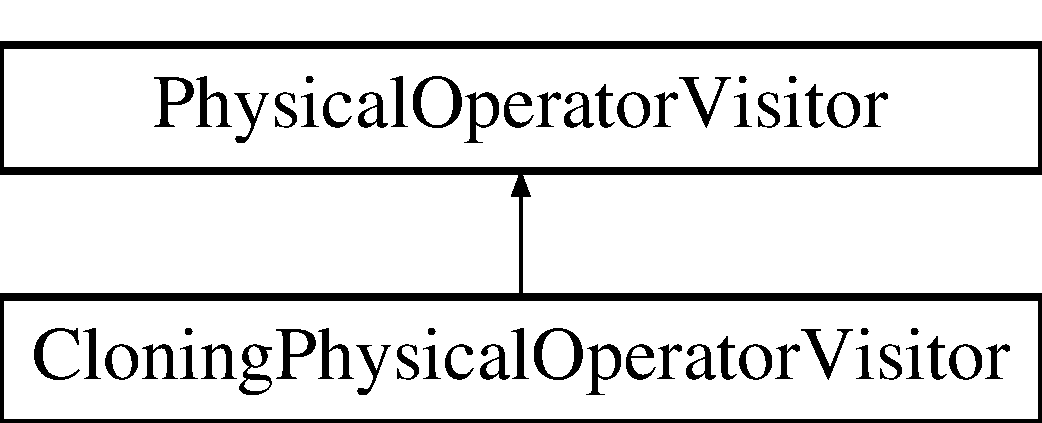
\includegraphics[height=2.000000cm]{class_cloning_physical_operator_visitor}
\end{center}
\end{figure}
\subsection*{Public Member Functions}
\begin{DoxyCompactItemize}
\item 
void \hyperlink{class_cloning_physical_operator_visitor_ac1b811ff2fd316b05d64f85c2e87fd9c}{visit\+Filter} (\hyperlink{class_filter}{Filter} $\ast$node)
\item 
void \hyperlink{class_cloning_physical_operator_visitor_a41aff61c8da3a7b88beddb6aaffb211e}{visit\+Filter\+Keeping\+Order} (\hyperlink{class_filter_keeping_order}{Filter\+Keeping\+Order} $\ast$node)
\item 
void \hyperlink{class_cloning_physical_operator_visitor_a5bb911312d752fcc31b48bb21f658bdf}{visit\+Sort\+Operator} (\hyperlink{class_sort_operator}{Sort\+Operator} $\ast$node)
\item 
void \hyperlink{class_cloning_physical_operator_visitor_ae1eb095ee91c30030c7830a9b999a6ec}{visit\+Merge\+Equi\+Join} (\hyperlink{class_merge_equi_join}{Merge\+Equi\+Join} $\ast$node)
\item 
void \hyperlink{class_cloning_physical_operator_visitor_a6b17fd37e070917db7152f869517eb4a}{visit\+Merge\+Non\+Equi\+Join} (\hyperlink{class_merge_non_equi_join}{Merge\+Non\+Equi\+Join} $\ast$node)
\item 
void \hyperlink{class_cloning_physical_operator_visitor_aa48e6141645ce53d8cae2b1678fdc2d4}{visit\+Cross\+Join} (\hyperlink{class_cross_join}{Cross\+Join} $\ast$node)
\item 
void \hyperlink{class_cloning_physical_operator_visitor_abb1f8426172480eb5968abd7f9deb541}{visit\+Hash\+Join} (\hyperlink{class_hash_join}{Hash\+Join} $\ast$node)
\item 
void \hyperlink{class_cloning_physical_operator_visitor_a661c04bfbdf0d36e745fc82bf8f8a193}{visit\+Hash\+Anti\+Join} (\hyperlink{class_hash_anti_join}{Hash\+Anti\+Join} $\ast$node)
\item 
void \hyperlink{class_cloning_physical_operator_visitor_af32410ddcbf200eb102bbe8ad5ad1859}{visit\+Merge\+Anti\+Join} (\hyperlink{class_merge_anti_join}{Merge\+Anti\+Join} $\ast$node)
\item 
void \hyperlink{class_cloning_physical_operator_visitor_af9199524feba8c12ceff7d78c1915064}{visit\+Union\+Operator} (\hyperlink{class_union_operator}{Union\+Operator} $\ast$node)
\item 
void \hyperlink{class_cloning_physical_operator_visitor_aa3a6b9d8327700089089e57e18861d6d}{visit\+Hash\+Group} (\hyperlink{class_hash_group}{Hash\+Group} $\ast$node)
\item 
void \hyperlink{class_cloning_physical_operator_visitor_a464894a18b7194c57e0c8d16f901ff5b}{visit\+Sorted\+Group} (\hyperlink{class_sorted_group}{Sorted\+Group} $\ast$node)
\item 
void \hyperlink{class_cloning_physical_operator_visitor_ad818258fa87a049e49d255107f655819}{visit\+Columns\+Operations\+Operator} (\hyperlink{class_columns_operations_operator}{Columns\+Operations\+Operator} $\ast$node)
\item 
void \hyperlink{class_cloning_physical_operator_visitor_a5bead629c3b23b39316b8b86913617e7}{visit\+Scan\+And\+Sort\+By\+Index} (\hyperlink{class_scan_and_sort_by_index}{Scan\+And\+Sort\+By\+Index} $\ast$node)
\item 
void \hyperlink{class_cloning_physical_operator_visitor_aa7066c58c8963023737f1b8e0eca7bca}{visit\+Table\+Scan} (\hyperlink{class_table_scan}{Table\+Scan} $\ast$node)
\item 
void \hyperlink{class_cloning_physical_operator_visitor_ae5e119521bb2d4654eebba24bc469739}{visit\+Index\+Scan} (\hyperlink{class_index_scan}{Index\+Scan} $\ast$node)
\end{DoxyCompactItemize}
\subsection*{Public Attributes}
\begin{DoxyCompactItemize}
\item 
std\+::shared\+\_\+ptr$<$ \hyperlink{class_physical_operator}{Physical\+Operator} $>$ \hyperlink{class_cloning_physical_operator_visitor_aa3705b767976ef07fdfe39458543138e}{result}
\end{DoxyCompactItemize}


\subsection{Detailed Description}
Clones physial operator tree. 

\subsection{Member Function Documentation}
\hypertarget{class_cloning_physical_operator_visitor_ad818258fa87a049e49d255107f655819}{\index{Cloning\+Physical\+Operator\+Visitor@{Cloning\+Physical\+Operator\+Visitor}!visit\+Columns\+Operations\+Operator@{visit\+Columns\+Operations\+Operator}}
\index{visit\+Columns\+Operations\+Operator@{visit\+Columns\+Operations\+Operator}!Cloning\+Physical\+Operator\+Visitor@{Cloning\+Physical\+Operator\+Visitor}}
\subsubsection[{visit\+Columns\+Operations\+Operator}]{\setlength{\rightskip}{0pt plus 5cm}void Cloning\+Physical\+Operator\+Visitor\+::visit\+Columns\+Operations\+Operator (
\begin{DoxyParamCaption}
\item[{{\bf Columns\+Operations\+Operator} $\ast$}]{node}
\end{DoxyParamCaption}
)\hspace{0.3cm}{\ttfamily [virtual]}}}\label{class_cloning_physical_operator_visitor_ad818258fa87a049e49d255107f655819}
Visits physical operator \hyperlink{class_columns_operations_operator}{Columns\+Operations\+Operator}. 
\begin{DoxyParams}{Parameters}
{\em node} & visited \hyperlink{class_columns_operations_operator}{Columns\+Operations\+Operator}. \\
\hline
\end{DoxyParams}


Reimplemented from \hyperlink{class_physical_operator_visitor_a8c3a41665c8f7ce941532ad9d2052a14}{Physical\+Operator\+Visitor}.

\hypertarget{class_cloning_physical_operator_visitor_aa48e6141645ce53d8cae2b1678fdc2d4}{\index{Cloning\+Physical\+Operator\+Visitor@{Cloning\+Physical\+Operator\+Visitor}!visit\+Cross\+Join@{visit\+Cross\+Join}}
\index{visit\+Cross\+Join@{visit\+Cross\+Join}!Cloning\+Physical\+Operator\+Visitor@{Cloning\+Physical\+Operator\+Visitor}}
\subsubsection[{visit\+Cross\+Join}]{\setlength{\rightskip}{0pt plus 5cm}void Cloning\+Physical\+Operator\+Visitor\+::visit\+Cross\+Join (
\begin{DoxyParamCaption}
\item[{{\bf Cross\+Join} $\ast$}]{node}
\end{DoxyParamCaption}
)\hspace{0.3cm}{\ttfamily [virtual]}}}\label{class_cloning_physical_operator_visitor_aa48e6141645ce53d8cae2b1678fdc2d4}
Visits physical operator \hyperlink{class_cross_join}{Cross\+Join}. 
\begin{DoxyParams}{Parameters}
{\em node} & visited \hyperlink{class_cross_join}{Cross\+Join}. \\
\hline
\end{DoxyParams}


Reimplemented from \hyperlink{class_physical_operator_visitor_a897e543962a692f2725ff7742efae056}{Physical\+Operator\+Visitor}.

\hypertarget{class_cloning_physical_operator_visitor_ac1b811ff2fd316b05d64f85c2e87fd9c}{\index{Cloning\+Physical\+Operator\+Visitor@{Cloning\+Physical\+Operator\+Visitor}!visit\+Filter@{visit\+Filter}}
\index{visit\+Filter@{visit\+Filter}!Cloning\+Physical\+Operator\+Visitor@{Cloning\+Physical\+Operator\+Visitor}}
\subsubsection[{visit\+Filter}]{\setlength{\rightskip}{0pt plus 5cm}void Cloning\+Physical\+Operator\+Visitor\+::visit\+Filter (
\begin{DoxyParamCaption}
\item[{{\bf Filter} $\ast$}]{node}
\end{DoxyParamCaption}
)\hspace{0.3cm}{\ttfamily [virtual]}}}\label{class_cloning_physical_operator_visitor_ac1b811ff2fd316b05d64f85c2e87fd9c}
Visits physical operator \hyperlink{class_filter}{Filter}. 
\begin{DoxyParams}{Parameters}
{\em node} & visited \hyperlink{class_filter}{Filter}. \\
\hline
\end{DoxyParams}


Reimplemented from \hyperlink{class_physical_operator_visitor_a30731ff26547314b268e1166f10e57ee}{Physical\+Operator\+Visitor}.

\hypertarget{class_cloning_physical_operator_visitor_a41aff61c8da3a7b88beddb6aaffb211e}{\index{Cloning\+Physical\+Operator\+Visitor@{Cloning\+Physical\+Operator\+Visitor}!visit\+Filter\+Keeping\+Order@{visit\+Filter\+Keeping\+Order}}
\index{visit\+Filter\+Keeping\+Order@{visit\+Filter\+Keeping\+Order}!Cloning\+Physical\+Operator\+Visitor@{Cloning\+Physical\+Operator\+Visitor}}
\subsubsection[{visit\+Filter\+Keeping\+Order}]{\setlength{\rightskip}{0pt plus 5cm}void Cloning\+Physical\+Operator\+Visitor\+::visit\+Filter\+Keeping\+Order (
\begin{DoxyParamCaption}
\item[{{\bf Filter\+Keeping\+Order} $\ast$}]{node}
\end{DoxyParamCaption}
)\hspace{0.3cm}{\ttfamily [virtual]}}}\label{class_cloning_physical_operator_visitor_a41aff61c8da3a7b88beddb6aaffb211e}
Visits physical operator \hyperlink{class_filter_keeping_order}{Filter\+Keeping\+Order}. 
\begin{DoxyParams}{Parameters}
{\em node} & visited \hyperlink{class_filter_keeping_order}{Filter\+Keeping\+Order}. \\
\hline
\end{DoxyParams}


Reimplemented from \hyperlink{class_physical_operator_visitor_a87aa256f7633364ab8fea61a4a20dd19}{Physical\+Operator\+Visitor}.

\hypertarget{class_cloning_physical_operator_visitor_a661c04bfbdf0d36e745fc82bf8f8a193}{\index{Cloning\+Physical\+Operator\+Visitor@{Cloning\+Physical\+Operator\+Visitor}!visit\+Hash\+Anti\+Join@{visit\+Hash\+Anti\+Join}}
\index{visit\+Hash\+Anti\+Join@{visit\+Hash\+Anti\+Join}!Cloning\+Physical\+Operator\+Visitor@{Cloning\+Physical\+Operator\+Visitor}}
\subsubsection[{visit\+Hash\+Anti\+Join}]{\setlength{\rightskip}{0pt plus 5cm}void Cloning\+Physical\+Operator\+Visitor\+::visit\+Hash\+Anti\+Join (
\begin{DoxyParamCaption}
\item[{{\bf Hash\+Anti\+Join} $\ast$}]{node}
\end{DoxyParamCaption}
)\hspace{0.3cm}{\ttfamily [virtual]}}}\label{class_cloning_physical_operator_visitor_a661c04bfbdf0d36e745fc82bf8f8a193}
Visits physical operator \hyperlink{class_hash_anti_join}{Hash\+Anti\+Join}. 
\begin{DoxyParams}{Parameters}
{\em node} & visited \hyperlink{class_hash_anti_join}{Hash\+Anti\+Join}. \\
\hline
\end{DoxyParams}


Reimplemented from \hyperlink{class_physical_operator_visitor_af1ce499e2c6db52ed03c3e5f57d144d3}{Physical\+Operator\+Visitor}.

\hypertarget{class_cloning_physical_operator_visitor_aa3a6b9d8327700089089e57e18861d6d}{\index{Cloning\+Physical\+Operator\+Visitor@{Cloning\+Physical\+Operator\+Visitor}!visit\+Hash\+Group@{visit\+Hash\+Group}}
\index{visit\+Hash\+Group@{visit\+Hash\+Group}!Cloning\+Physical\+Operator\+Visitor@{Cloning\+Physical\+Operator\+Visitor}}
\subsubsection[{visit\+Hash\+Group}]{\setlength{\rightskip}{0pt plus 5cm}void Cloning\+Physical\+Operator\+Visitor\+::visit\+Hash\+Group (
\begin{DoxyParamCaption}
\item[{{\bf Hash\+Group} $\ast$}]{node}
\end{DoxyParamCaption}
)\hspace{0.3cm}{\ttfamily [virtual]}}}\label{class_cloning_physical_operator_visitor_aa3a6b9d8327700089089e57e18861d6d}
Visits physical operator \hyperlink{class_hash_group}{Hash\+Group}. 
\begin{DoxyParams}{Parameters}
{\em node} & visited \hyperlink{class_hash_group}{Hash\+Group}. \\
\hline
\end{DoxyParams}


Reimplemented from \hyperlink{class_physical_operator_visitor_aa5591d034ce34887c813affc48b7a19c}{Physical\+Operator\+Visitor}.

\hypertarget{class_cloning_physical_operator_visitor_abb1f8426172480eb5968abd7f9deb541}{\index{Cloning\+Physical\+Operator\+Visitor@{Cloning\+Physical\+Operator\+Visitor}!visit\+Hash\+Join@{visit\+Hash\+Join}}
\index{visit\+Hash\+Join@{visit\+Hash\+Join}!Cloning\+Physical\+Operator\+Visitor@{Cloning\+Physical\+Operator\+Visitor}}
\subsubsection[{visit\+Hash\+Join}]{\setlength{\rightskip}{0pt plus 5cm}void Cloning\+Physical\+Operator\+Visitor\+::visit\+Hash\+Join (
\begin{DoxyParamCaption}
\item[{{\bf Hash\+Join} $\ast$}]{node}
\end{DoxyParamCaption}
)\hspace{0.3cm}{\ttfamily [virtual]}}}\label{class_cloning_physical_operator_visitor_abb1f8426172480eb5968abd7f9deb541}
Visits physical operator \hyperlink{class_hash_join}{Hash\+Join}. 
\begin{DoxyParams}{Parameters}
{\em node} & visited \hyperlink{class_hash_join}{Hash\+Join}. \\
\hline
\end{DoxyParams}


Reimplemented from \hyperlink{class_physical_operator_visitor_aedb5da87c0637ad8097b7c2eb129129e}{Physical\+Operator\+Visitor}.

\hypertarget{class_cloning_physical_operator_visitor_ae5e119521bb2d4654eebba24bc469739}{\index{Cloning\+Physical\+Operator\+Visitor@{Cloning\+Physical\+Operator\+Visitor}!visit\+Index\+Scan@{visit\+Index\+Scan}}
\index{visit\+Index\+Scan@{visit\+Index\+Scan}!Cloning\+Physical\+Operator\+Visitor@{Cloning\+Physical\+Operator\+Visitor}}
\subsubsection[{visit\+Index\+Scan}]{\setlength{\rightskip}{0pt plus 5cm}void Cloning\+Physical\+Operator\+Visitor\+::visit\+Index\+Scan (
\begin{DoxyParamCaption}
\item[{{\bf Index\+Scan} $\ast$}]{node}
\end{DoxyParamCaption}
)\hspace{0.3cm}{\ttfamily [virtual]}}}\label{class_cloning_physical_operator_visitor_ae5e119521bb2d4654eebba24bc469739}
Visits physical operator \hyperlink{class_index_scan}{Index\+Scan}. 
\begin{DoxyParams}{Parameters}
{\em node} & visited \hyperlink{class_index_scan}{Index\+Scan}. \\
\hline
\end{DoxyParams}


Reimplemented from \hyperlink{class_physical_operator_visitor_ae32578d3229a00be39229a86b575c599}{Physical\+Operator\+Visitor}.

\hypertarget{class_cloning_physical_operator_visitor_af32410ddcbf200eb102bbe8ad5ad1859}{\index{Cloning\+Physical\+Operator\+Visitor@{Cloning\+Physical\+Operator\+Visitor}!visit\+Merge\+Anti\+Join@{visit\+Merge\+Anti\+Join}}
\index{visit\+Merge\+Anti\+Join@{visit\+Merge\+Anti\+Join}!Cloning\+Physical\+Operator\+Visitor@{Cloning\+Physical\+Operator\+Visitor}}
\subsubsection[{visit\+Merge\+Anti\+Join}]{\setlength{\rightskip}{0pt plus 5cm}void Cloning\+Physical\+Operator\+Visitor\+::visit\+Merge\+Anti\+Join (
\begin{DoxyParamCaption}
\item[{{\bf Merge\+Anti\+Join} $\ast$}]{node}
\end{DoxyParamCaption}
)\hspace{0.3cm}{\ttfamily [virtual]}}}\label{class_cloning_physical_operator_visitor_af32410ddcbf200eb102bbe8ad5ad1859}
Visits physical operator \hyperlink{class_merge_anti_join}{Merge\+Anti\+Join}. 
\begin{DoxyParams}{Parameters}
{\em node} & visited \hyperlink{class_merge_anti_join}{Merge\+Anti\+Join}. \\
\hline
\end{DoxyParams}


Reimplemented from \hyperlink{class_physical_operator_visitor_a3d44b3e23abc47c8c0c56938c12ed98a}{Physical\+Operator\+Visitor}.

\hypertarget{class_cloning_physical_operator_visitor_ae1eb095ee91c30030c7830a9b999a6ec}{\index{Cloning\+Physical\+Operator\+Visitor@{Cloning\+Physical\+Operator\+Visitor}!visit\+Merge\+Equi\+Join@{visit\+Merge\+Equi\+Join}}
\index{visit\+Merge\+Equi\+Join@{visit\+Merge\+Equi\+Join}!Cloning\+Physical\+Operator\+Visitor@{Cloning\+Physical\+Operator\+Visitor}}
\subsubsection[{visit\+Merge\+Equi\+Join}]{\setlength{\rightskip}{0pt plus 5cm}void Cloning\+Physical\+Operator\+Visitor\+::visit\+Merge\+Equi\+Join (
\begin{DoxyParamCaption}
\item[{{\bf Merge\+Equi\+Join} $\ast$}]{node}
\end{DoxyParamCaption}
)\hspace{0.3cm}{\ttfamily [virtual]}}}\label{class_cloning_physical_operator_visitor_ae1eb095ee91c30030c7830a9b999a6ec}
Visits physical operator \hyperlink{class_merge_equi_join}{Merge\+Equi\+Join}. 
\begin{DoxyParams}{Parameters}
{\em node} & visited \hyperlink{class_merge_equi_join}{Merge\+Equi\+Join}. \\
\hline
\end{DoxyParams}


Reimplemented from \hyperlink{class_physical_operator_visitor_a4a90fb4cad8fe3ab4877f6ee6f43e1e5}{Physical\+Operator\+Visitor}.

\hypertarget{class_cloning_physical_operator_visitor_a6b17fd37e070917db7152f869517eb4a}{\index{Cloning\+Physical\+Operator\+Visitor@{Cloning\+Physical\+Operator\+Visitor}!visit\+Merge\+Non\+Equi\+Join@{visit\+Merge\+Non\+Equi\+Join}}
\index{visit\+Merge\+Non\+Equi\+Join@{visit\+Merge\+Non\+Equi\+Join}!Cloning\+Physical\+Operator\+Visitor@{Cloning\+Physical\+Operator\+Visitor}}
\subsubsection[{visit\+Merge\+Non\+Equi\+Join}]{\setlength{\rightskip}{0pt plus 5cm}void Cloning\+Physical\+Operator\+Visitor\+::visit\+Merge\+Non\+Equi\+Join (
\begin{DoxyParamCaption}
\item[{{\bf Merge\+Non\+Equi\+Join} $\ast$}]{node}
\end{DoxyParamCaption}
)\hspace{0.3cm}{\ttfamily [virtual]}}}\label{class_cloning_physical_operator_visitor_a6b17fd37e070917db7152f869517eb4a}
Visits physical operator \hyperlink{class_merge_non_equi_join}{Merge\+Non\+Equi\+Join}. 
\begin{DoxyParams}{Parameters}
{\em node} & visited \hyperlink{class_merge_non_equi_join}{Merge\+Non\+Equi\+Join}. \\
\hline
\end{DoxyParams}


Reimplemented from \hyperlink{class_physical_operator_visitor_a9f8bd69369f2fff2bbc74b7aadceaab5}{Physical\+Operator\+Visitor}.

\hypertarget{class_cloning_physical_operator_visitor_a5bead629c3b23b39316b8b86913617e7}{\index{Cloning\+Physical\+Operator\+Visitor@{Cloning\+Physical\+Operator\+Visitor}!visit\+Scan\+And\+Sort\+By\+Index@{visit\+Scan\+And\+Sort\+By\+Index}}
\index{visit\+Scan\+And\+Sort\+By\+Index@{visit\+Scan\+And\+Sort\+By\+Index}!Cloning\+Physical\+Operator\+Visitor@{Cloning\+Physical\+Operator\+Visitor}}
\subsubsection[{visit\+Scan\+And\+Sort\+By\+Index}]{\setlength{\rightskip}{0pt plus 5cm}void Cloning\+Physical\+Operator\+Visitor\+::visit\+Scan\+And\+Sort\+By\+Index (
\begin{DoxyParamCaption}
\item[{{\bf Scan\+And\+Sort\+By\+Index} $\ast$}]{node}
\end{DoxyParamCaption}
)\hspace{0.3cm}{\ttfamily [virtual]}}}\label{class_cloning_physical_operator_visitor_a5bead629c3b23b39316b8b86913617e7}
Visits physical operator \hyperlink{class_scan_and_sort_by_index}{Scan\+And\+Sort\+By\+Index}. 
\begin{DoxyParams}{Parameters}
{\em node} & visited \hyperlink{class_scan_and_sort_by_index}{Scan\+And\+Sort\+By\+Index}. \\
\hline
\end{DoxyParams}


Reimplemented from \hyperlink{class_physical_operator_visitor_ad5551e62c8b00b676577ac6b046be696}{Physical\+Operator\+Visitor}.

\hypertarget{class_cloning_physical_operator_visitor_a464894a18b7194c57e0c8d16f901ff5b}{\index{Cloning\+Physical\+Operator\+Visitor@{Cloning\+Physical\+Operator\+Visitor}!visit\+Sorted\+Group@{visit\+Sorted\+Group}}
\index{visit\+Sorted\+Group@{visit\+Sorted\+Group}!Cloning\+Physical\+Operator\+Visitor@{Cloning\+Physical\+Operator\+Visitor}}
\subsubsection[{visit\+Sorted\+Group}]{\setlength{\rightskip}{0pt plus 5cm}void Cloning\+Physical\+Operator\+Visitor\+::visit\+Sorted\+Group (
\begin{DoxyParamCaption}
\item[{{\bf Sorted\+Group} $\ast$}]{node}
\end{DoxyParamCaption}
)\hspace{0.3cm}{\ttfamily [virtual]}}}\label{class_cloning_physical_operator_visitor_a464894a18b7194c57e0c8d16f901ff5b}
Visits physical operator \hyperlink{class_sorted_group}{Sorted\+Group}. 
\begin{DoxyParams}{Parameters}
{\em node} & visited \hyperlink{class_sorted_group}{Sorted\+Group}. \\
\hline
\end{DoxyParams}


Reimplemented from \hyperlink{class_physical_operator_visitor_a3a3499a62341acf3e49f34ee02a8ed61}{Physical\+Operator\+Visitor}.

\hypertarget{class_cloning_physical_operator_visitor_a5bb911312d752fcc31b48bb21f658bdf}{\index{Cloning\+Physical\+Operator\+Visitor@{Cloning\+Physical\+Operator\+Visitor}!visit\+Sort\+Operator@{visit\+Sort\+Operator}}
\index{visit\+Sort\+Operator@{visit\+Sort\+Operator}!Cloning\+Physical\+Operator\+Visitor@{Cloning\+Physical\+Operator\+Visitor}}
\subsubsection[{visit\+Sort\+Operator}]{\setlength{\rightskip}{0pt plus 5cm}void Cloning\+Physical\+Operator\+Visitor\+::visit\+Sort\+Operator (
\begin{DoxyParamCaption}
\item[{{\bf Sort\+Operator} $\ast$}]{node}
\end{DoxyParamCaption}
)\hspace{0.3cm}{\ttfamily [virtual]}}}\label{class_cloning_physical_operator_visitor_a5bb911312d752fcc31b48bb21f658bdf}
Visits physical operator \hyperlink{class_sort_operator}{Sort\+Operator}. 
\begin{DoxyParams}{Parameters}
{\em node} & visited \hyperlink{class_sort_operator}{Sort\+Operator}. \\
\hline
\end{DoxyParams}


Reimplemented from \hyperlink{class_physical_operator_visitor_ae5f81c64ca3acfa04737fc6655d72767}{Physical\+Operator\+Visitor}.

\hypertarget{class_cloning_physical_operator_visitor_aa7066c58c8963023737f1b8e0eca7bca}{\index{Cloning\+Physical\+Operator\+Visitor@{Cloning\+Physical\+Operator\+Visitor}!visit\+Table\+Scan@{visit\+Table\+Scan}}
\index{visit\+Table\+Scan@{visit\+Table\+Scan}!Cloning\+Physical\+Operator\+Visitor@{Cloning\+Physical\+Operator\+Visitor}}
\subsubsection[{visit\+Table\+Scan}]{\setlength{\rightskip}{0pt plus 5cm}void Cloning\+Physical\+Operator\+Visitor\+::visit\+Table\+Scan (
\begin{DoxyParamCaption}
\item[{{\bf Table\+Scan} $\ast$}]{node}
\end{DoxyParamCaption}
)\hspace{0.3cm}{\ttfamily [virtual]}}}\label{class_cloning_physical_operator_visitor_aa7066c58c8963023737f1b8e0eca7bca}
Visits physical operator \hyperlink{class_table_scan}{Table\+Scan}. 
\begin{DoxyParams}{Parameters}
{\em node} & visited \hyperlink{class_table_scan}{Table\+Scan}. \\
\hline
\end{DoxyParams}


Reimplemented from \hyperlink{class_physical_operator_visitor_a62063b4a4740e730ef7f6728dd926d52}{Physical\+Operator\+Visitor}.

\hypertarget{class_cloning_physical_operator_visitor_af9199524feba8c12ceff7d78c1915064}{\index{Cloning\+Physical\+Operator\+Visitor@{Cloning\+Physical\+Operator\+Visitor}!visit\+Union\+Operator@{visit\+Union\+Operator}}
\index{visit\+Union\+Operator@{visit\+Union\+Operator}!Cloning\+Physical\+Operator\+Visitor@{Cloning\+Physical\+Operator\+Visitor}}
\subsubsection[{visit\+Union\+Operator}]{\setlength{\rightskip}{0pt plus 5cm}void Cloning\+Physical\+Operator\+Visitor\+::visit\+Union\+Operator (
\begin{DoxyParamCaption}
\item[{{\bf Union\+Operator} $\ast$}]{node}
\end{DoxyParamCaption}
)\hspace{0.3cm}{\ttfamily [virtual]}}}\label{class_cloning_physical_operator_visitor_af9199524feba8c12ceff7d78c1915064}
Visits physical operator \hyperlink{class_union_operator}{Union\+Operator}. 
\begin{DoxyParams}{Parameters}
{\em node} & visited \hyperlink{class_union_operator}{Union\+Operator}. \\
\hline
\end{DoxyParams}


Reimplemented from \hyperlink{class_physical_operator_visitor_adbb3e6618904bc7e6d0b6aa3958132e9}{Physical\+Operator\+Visitor}.



\subsection{Member Data Documentation}
\hypertarget{class_cloning_physical_operator_visitor_aa3705b767976ef07fdfe39458543138e}{\index{Cloning\+Physical\+Operator\+Visitor@{Cloning\+Physical\+Operator\+Visitor}!result@{result}}
\index{result@{result}!Cloning\+Physical\+Operator\+Visitor@{Cloning\+Physical\+Operator\+Visitor}}
\subsubsection[{result}]{\setlength{\rightskip}{0pt plus 5cm}std\+::shared\+\_\+ptr$<${\bf Physical\+Operator}$>$ Cloning\+Physical\+Operator\+Visitor\+::result}}\label{class_cloning_physical_operator_visitor_aa3705b767976ef07fdfe39458543138e}
Cloned result. 

The documentation for this class was generated from the following files\+:\begin{DoxyCompactItemize}
\item 
C\+:/\+Users/\+Marcel/\+Documents/\+Visual Studio 2012/\+Projects/\+Relational\+Query\+Evaluator/\+Relational\+Query\+Evaluator/Physical\+Operator\+Visitor.\+h\item 
C\+:/\+Users/\+Marcel/\+Documents/\+Visual Studio 2012/\+Projects/\+Relational\+Query\+Evaluator/\+Relational\+Query\+Evaluator/Physical\+Operator\+Visitor.\+cpp\end{DoxyCompactItemize}

\hypertarget{class_column}{\section{Column Class Reference}
\label{class_column}\index{Column@{Column}}
}
Inheritance diagram for Column\+:\begin{figure}[H]
\begin{center}
\leavevmode
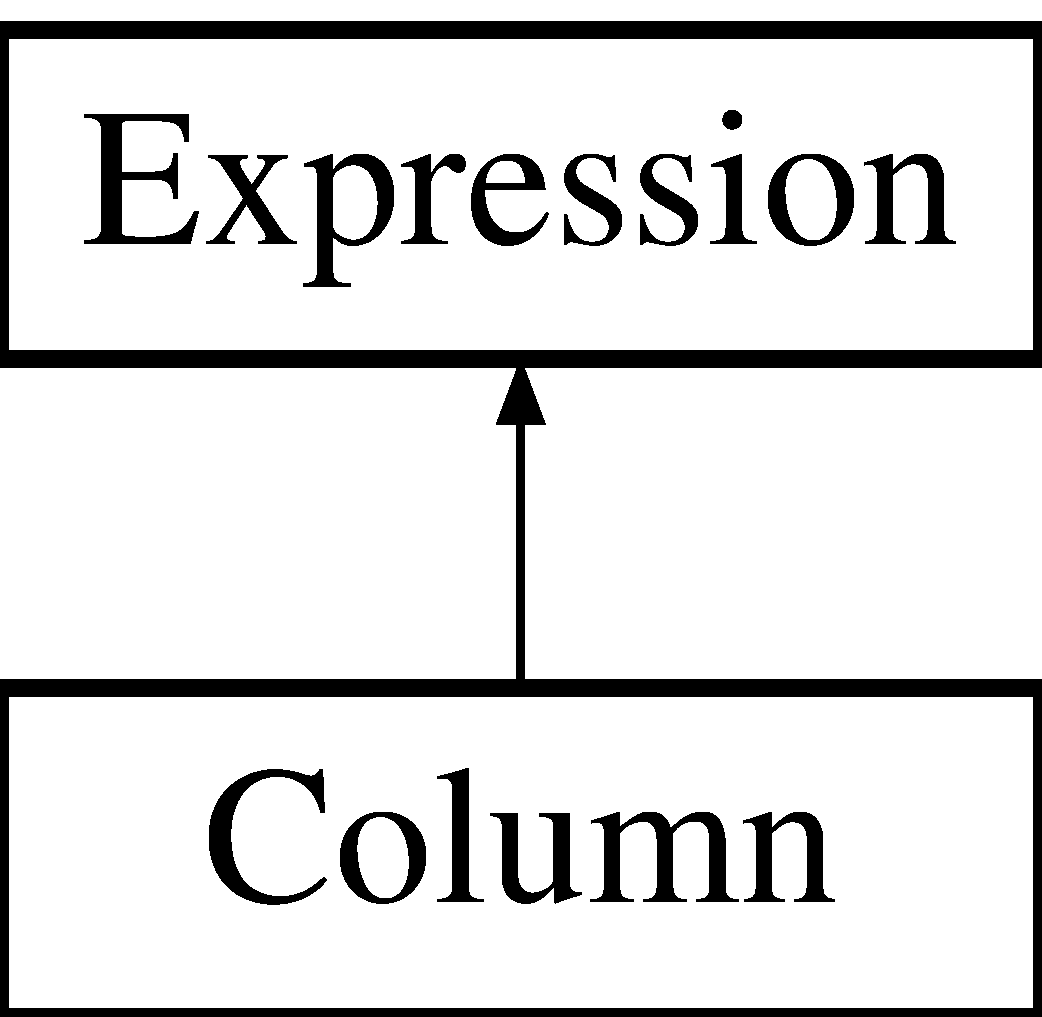
\includegraphics[height=2.000000cm]{class_column}
\end{center}
\end{figure}
\subsection*{Public Member Functions}
\begin{DoxyCompactItemize}
\item 
\hypertarget{class_column_a9934481a60fd2373bfe7ced5f208b505}{{\bfseries Column} (D\+O\+M\+Element $\ast$node)}\label{class_column_a9934481a60fd2373bfe7ced5f208b505}

\item 
\hypertarget{class_column_a6e925985b1e87ed92795d318c52e5470}{void {\bfseries accept} (\hyperlink{class_expression_visitor_base}{Expression\+Visitor\+Base} \&v)}\label{class_column_a6e925985b1e87ed92795d318c52e5470}

\item 
\hypertarget{class_column_af1571fb51f887aeb1dcf7ff44382a72b}{void {\bfseries replace\+Child} (\hyperlink{class_expression}{Expression} $\ast$old\+Child, std\+::shared\+\_\+ptr$<$ \hyperlink{class_expression}{Expression} $>$ new\+Child)}\label{class_column_af1571fb51f887aeb1dcf7ff44382a72b}

\end{DoxyCompactItemize}
\subsection*{Public Attributes}
\begin{DoxyCompactItemize}
\item 
\hypertarget{class_column_a22e87a2e1f67da45c085a9898156e31c}{\hyperlink{class_column_identifier}{Column\+Identifier} {\bfseries column}}\label{class_column_a22e87a2e1f67da45c085a9898156e31c}

\item 
\hypertarget{class_column_a18cd6b6f12a338f6e08c36da7fadb7ec}{std\+::string {\bfseries type}}\label{class_column_a18cd6b6f12a338f6e08c36da7fadb7ec}

\item 
\hypertarget{class_column_addd3816c69df05b9f717348dca79ee21}{ulong {\bfseries input}}\label{class_column_addd3816c69df05b9f717348dca79ee21}

\end{DoxyCompactItemize}
\subsection*{Additional Inherited Members}


The documentation for this class was generated from the following files\+:\begin{DoxyCompactItemize}
\item 
C\+:/\+Users/\+Marcel/\+Documents/\+Visual Studio 2012/\+Projects/\+Relational\+Query\+Evaluator/\+Relational\+Query\+Evaluator/Expressions.\+h\item 
C\+:/\+Users/\+Marcel/\+Documents/\+Visual Studio 2012/\+Projects/\+Relational\+Query\+Evaluator/\+Relational\+Query\+Evaluator/Expressions.\+cpp\end{DoxyCompactItemize}

\hypertarget{class_column_identifier}{\section{Column\+Identifier Class Reference}
\label{class_column_identifier}\index{Column\+Identifier@{Column\+Identifier}}
}
\subsection*{Public Member Functions}
\begin{DoxyCompactItemize}
\item 
\hypertarget{class_column_identifier_a3fae121a889e26575b1b2e6ebad16d6e}{{\bfseries Column\+Identifier} (std\+::string name, int id)}\label{class_column_identifier_a3fae121a889e26575b1b2e6ebad16d6e}

\item 
\hypertarget{class_column_identifier_ac9bd3a91e6e885751182d082b28d5fb0}{{\bfseries Column\+Identifier} (std\+::string name)}\label{class_column_identifier_ac9bd3a91e6e885751182d082b28d5fb0}

\item 
\hypertarget{class_column_identifier_ae6b2e2ce0ac26d356a451ec3d975a1be}{std\+::string {\bfseries to\+String} () const }\label{class_column_identifier_ae6b2e2ce0ac26d356a451ec3d975a1be}

\item 
\hypertarget{class_column_identifier_a07e32ed45a2b7c8e09f0358fd31a1f74}{bool {\bfseries operator$<$} (const \hyperlink{class_column_identifier}{Column\+Identifier} \&other) const }\label{class_column_identifier_a07e32ed45a2b7c8e09f0358fd31a1f74}

\item 
\hypertarget{class_column_identifier_a3833af96f5281573cae9a70c440c1cce}{bool {\bfseries operator==} (const \hyperlink{class_column_identifier}{Column\+Identifier} \&other) const }\label{class_column_identifier_a3833af96f5281573cae9a70c440c1cce}

\end{DoxyCompactItemize}
\subsection*{Public Attributes}
\begin{DoxyCompactItemize}
\item 
\hypertarget{class_column_identifier_af401adcef91c0fb4087102182dddb6ea}{std\+::string {\bfseries name}}\label{class_column_identifier_af401adcef91c0fb4087102182dddb6ea}

\item 
\hypertarget{class_column_identifier_ade5213e0ceeb1ba3fd948e9dc9975a53}{int {\bfseries id}}\label{class_column_identifier_ade5213e0ceeb1ba3fd948e9dc9975a53}

\end{DoxyCompactItemize}


The documentation for this class was generated from the following files\+:\begin{DoxyCompactItemize}
\item 
C\+:/\+Users/\+Marcel/\+Documents/\+Visual Studio 2012/\+Projects/\+Relational\+Query\+Evaluator/\+Relational\+Query\+Evaluator/Algebra\+Structures.\+h\item 
C\+:/\+Users/\+Marcel/\+Documents/\+Visual Studio 2012/\+Projects/\+Relational\+Query\+Evaluator/\+Relational\+Query\+Evaluator/Algebra\+Structures.\+cpp\end{DoxyCompactItemize}

\hypertarget{class_column_info}{\section{Column\+Info Class Reference}
\label{class_column_info}\index{Column\+Info@{Column\+Info}}
}


{\ttfamily \#include $<$Algebra\+Structures.\+h$>$}

Inheritance diagram for Column\+Info\+:\begin{figure}[H]
\begin{center}
\leavevmode
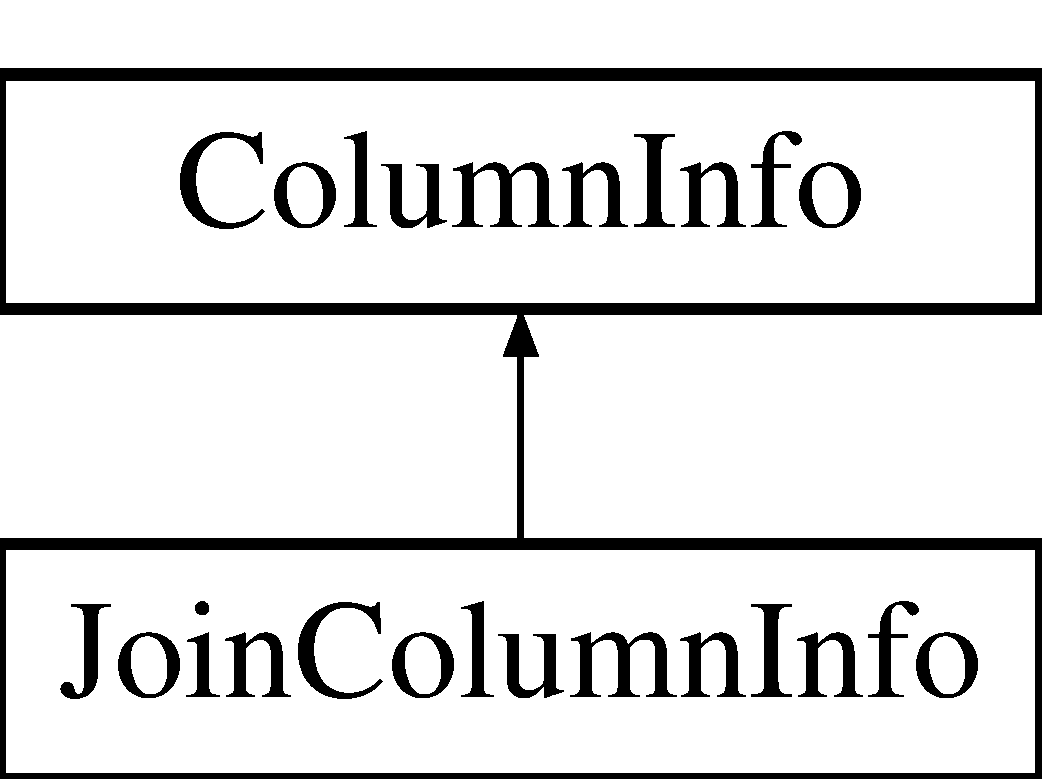
\includegraphics[height=2.000000cm]{class_column_info}
\end{center}
\end{figure}
\subsection*{Public Member Functions}
\begin{DoxyCompactItemize}
\item 
\hyperlink{class_column_info_a1068047ba3c85b84076e69619f64123a}{Column\+Info} (std\+::string name, std\+::string \hyperlink{class_column_info_add303d9d4415fc18b790d9a904831c29}{type})
\item 
\hyperlink{class_column_info_a12b2dd59f7b6c13008291c3ef03ba7f4}{Column\+Info} ()
\item 
\hyperlink{class_column_info_ae8dc9720185a9312e3b33b2ecb92ba7e}{Column\+Info} (std\+::string name, double \hyperlink{class_column_info_add402bfa7bed26aa6072c5da9b06dda9}{number\+Of\+Unique\+Values}, std\+::string \hyperlink{class_column_info_add303d9d4415fc18b790d9a904831c29}{type})
\item 
\hyperlink{class_column_info_a64cd8f7c77b3fe41434b85b05fa88344}{Column\+Info} (const \hyperlink{class_column_identifier}{Column\+Identifier} \&\hyperlink{class_column_info_a13c87a82665272f3eb3e18a8323d0d7e}{column}, double \hyperlink{class_column_info_add402bfa7bed26aa6072c5da9b06dda9}{number\+Of\+Unique\+Values}, std\+::string \hyperlink{class_column_info_add303d9d4415fc18b790d9a904831c29}{type})
\item 
\hyperlink{class_column_info_af5487ed1e204fe47f66414f7570eb649}{Column\+Info} (const \hyperlink{class_join_column_info}{Join\+Column\+Info} \&info)
\end{DoxyCompactItemize}
\subsection*{Public Attributes}
\begin{DoxyCompactItemize}
\item 
\hyperlink{class_column_identifier}{Column\+Identifier} \hyperlink{class_column_info_a13c87a82665272f3eb3e18a8323d0d7e}{column}
\item 
std\+::string \hyperlink{class_column_info_add303d9d4415fc18b790d9a904831c29}{type}
\item 
double \hyperlink{class_column_info_add402bfa7bed26aa6072c5da9b06dda9}{number\+Of\+Unique\+Values}
\end{DoxyCompactItemize}


\subsection{Detailed Description}
Stored information about column, like identifier, number of uniquevalues and type. 

\subsection{Constructor \& Destructor Documentation}
\hypertarget{class_column_info_a1068047ba3c85b84076e69619f64123a}{\index{Column\+Info@{Column\+Info}!Column\+Info@{Column\+Info}}
\index{Column\+Info@{Column\+Info}!Column\+Info@{Column\+Info}}
\subsubsection[{Column\+Info}]{\setlength{\rightskip}{0pt plus 5cm}Column\+Info\+::\+Column\+Info (
\begin{DoxyParamCaption}
\item[{std\+::string}]{name, }
\item[{std\+::string}]{type}
\end{DoxyParamCaption}
)}}\label{class_column_info_a1068047ba3c85b84076e69619f64123a}
Create the instance of \hyperlink{class_column_info}{Column\+Info}. 
\begin{DoxyParams}{Parameters}
{\em name} & -\/ column name \\
\hline
{\em type} & -\/ column type \\
\hline
\end{DoxyParams}
\hypertarget{class_column_info_a12b2dd59f7b6c13008291c3ef03ba7f4}{\index{Column\+Info@{Column\+Info}!Column\+Info@{Column\+Info}}
\index{Column\+Info@{Column\+Info}!Column\+Info@{Column\+Info}}
\subsubsection[{Column\+Info}]{\setlength{\rightskip}{0pt plus 5cm}Column\+Info\+::\+Column\+Info (
\begin{DoxyParamCaption}
{}
\end{DoxyParamCaption}
)}}\label{class_column_info_a12b2dd59f7b6c13008291c3ef03ba7f4}
Create the instance of \hyperlink{class_column_info}{Column\+Info}. \hypertarget{class_column_info_ae8dc9720185a9312e3b33b2ecb92ba7e}{\index{Column\+Info@{Column\+Info}!Column\+Info@{Column\+Info}}
\index{Column\+Info@{Column\+Info}!Column\+Info@{Column\+Info}}
\subsubsection[{Column\+Info}]{\setlength{\rightskip}{0pt plus 5cm}Column\+Info\+::\+Column\+Info (
\begin{DoxyParamCaption}
\item[{std\+::string}]{name, }
\item[{double}]{number\+Of\+Unique\+Values, }
\item[{std\+::string}]{type}
\end{DoxyParamCaption}
)}}\label{class_column_info_ae8dc9720185a9312e3b33b2ecb92ba7e}
Create the instance of \hyperlink{class_column_info}{Column\+Info}. 
\begin{DoxyParams}{Parameters}
{\em name} & -\/ column name \\
\hline
{\em number\+Of\+Unique\+Values} & \\
\hline
{\em type} & -\/ type of column \\
\hline
\end{DoxyParams}
\hypertarget{class_column_info_a64cd8f7c77b3fe41434b85b05fa88344}{\index{Column\+Info@{Column\+Info}!Column\+Info@{Column\+Info}}
\index{Column\+Info@{Column\+Info}!Column\+Info@{Column\+Info}}
\subsubsection[{Column\+Info}]{\setlength{\rightskip}{0pt plus 5cm}Column\+Info\+::\+Column\+Info (
\begin{DoxyParamCaption}
\item[{const {\bf Column\+Identifier} \&}]{column, }
\item[{double}]{number\+Of\+Unique\+Values, }
\item[{std\+::string}]{type}
\end{DoxyParamCaption}
)}}\label{class_column_info_a64cd8f7c77b3fe41434b85b05fa88344}
Create the instance of \hyperlink{class_column_info}{Column\+Info}. 
\begin{DoxyParams}{Parameters}
{\em column} & -\/ \hyperlink{class_column_identifier}{Column\+Identifier} of the column \\
\hline
{\em number\+Of\+Unique\+Values} & \\
\hline
{\em type} & -\/ type of column \\
\hline
\end{DoxyParams}
\hypertarget{class_column_info_af5487ed1e204fe47f66414f7570eb649}{\index{Column\+Info@{Column\+Info}!Column\+Info@{Column\+Info}}
\index{Column\+Info@{Column\+Info}!Column\+Info@{Column\+Info}}
\subsubsection[{Column\+Info}]{\setlength{\rightskip}{0pt plus 5cm}Column\+Info\+::\+Column\+Info (
\begin{DoxyParamCaption}
\item[{const {\bf Join\+Column\+Info} \&}]{info}
\end{DoxyParamCaption}
)}}\label{class_column_info_af5487ed1e204fe47f66414f7570eb649}
Create the instance of \hyperlink{class_column_info}{Column\+Info}. 
\begin{DoxyParams}{Parameters}
{\em info} & -\/ \hyperlink{class_join_column_info}{Join\+Column\+Info} \\
\hline
\end{DoxyParams}


\subsection{Member Data Documentation}
\hypertarget{class_column_info_a13c87a82665272f3eb3e18a8323d0d7e}{\index{Column\+Info@{Column\+Info}!column@{column}}
\index{column@{column}!Column\+Info@{Column\+Info}}
\subsubsection[{column}]{\setlength{\rightskip}{0pt plus 5cm}{\bf Column\+Identifier} Column\+Info\+::column}}\label{class_column_info_a13c87a82665272f3eb3e18a8323d0d7e}
Columns identifier. \hypertarget{class_column_info_add402bfa7bed26aa6072c5da9b06dda9}{\index{Column\+Info@{Column\+Info}!number\+Of\+Unique\+Values@{number\+Of\+Unique\+Values}}
\index{number\+Of\+Unique\+Values@{number\+Of\+Unique\+Values}!Column\+Info@{Column\+Info}}
\subsubsection[{number\+Of\+Unique\+Values}]{\setlength{\rightskip}{0pt plus 5cm}double Column\+Info\+::number\+Of\+Unique\+Values}}\label{class_column_info_add402bfa7bed26aa6072c5da9b06dda9}
Stores number of unique values for joining purposes. \hypertarget{class_column_info_add303d9d4415fc18b790d9a904831c29}{\index{Column\+Info@{Column\+Info}!type@{type}}
\index{type@{type}!Column\+Info@{Column\+Info}}
\subsubsection[{type}]{\setlength{\rightskip}{0pt plus 5cm}std\+::string Column\+Info\+::type}}\label{class_column_info_add303d9d4415fc18b790d9a904831c29}
Type of the column. 

The documentation for this class was generated from the following files\+:\begin{DoxyCompactItemize}
\item 
C\+:/\+Users/\+Marcel/\+Documents/\+Visual Studio 2012/\+Projects/\+Relational\+Query\+Evaluator/\+Relational\+Query\+Evaluator/Algebra\+Structures.\+h\item 
C\+:/\+Users/\+Marcel/\+Documents/\+Visual Studio 2012/\+Projects/\+Relational\+Query\+Evaluator/\+Relational\+Query\+Evaluator/Algebra\+Structures.\+cpp\end{DoxyCompactItemize}

\hypertarget{class_column_operation}{\section{Column\+Operation Class Reference}
\label{class_column_operation}\index{Column\+Operation@{Column\+Operation}}
}
\subsection*{Public Attributes}
\begin{DoxyCompactItemize}
\item 
\hypertarget{class_column_operation_aab22c48d83db533c5b153136a4da6db7}{\hyperlink{class_column_identifier}{Column\+Identifier} {\bfseries result}}\label{class_column_operation_aab22c48d83db533c5b153136a4da6db7}

\item 
\hypertarget{class_column_operation_a4d5d373009098230cb3a2bfa3aa3cc33}{std\+::shared\+\_\+ptr$<$ \hyperlink{class_expression}{Expression} $>$ {\bfseries expression}}\label{class_column_operation_a4d5d373009098230cb3a2bfa3aa3cc33}

\item 
\hypertarget{class_column_operation_ae04fd07588173c74291e80032f80f991}{std\+::string {\bfseries type}}\label{class_column_operation_ae04fd07588173c74291e80032f80f991}

\end{DoxyCompactItemize}


The documentation for this class was generated from the following file\+:\begin{DoxyCompactItemize}
\item 
C\+:/\+Users/\+Marcel/\+Documents/\+Visual Studio 2012/\+Projects/\+Relational\+Query\+Evaluator/\+Relational\+Query\+Evaluator/Algebra\+Structures.\+h\end{DoxyCompactItemize}

\hypertarget{class_column_operations}{\section{Column\+Operations Class Reference}
\label{class_column_operations}\index{Column\+Operations@{Column\+Operations}}
}
Inheritance diagram for Column\+Operations\+:\begin{figure}[H]
\begin{center}
\leavevmode
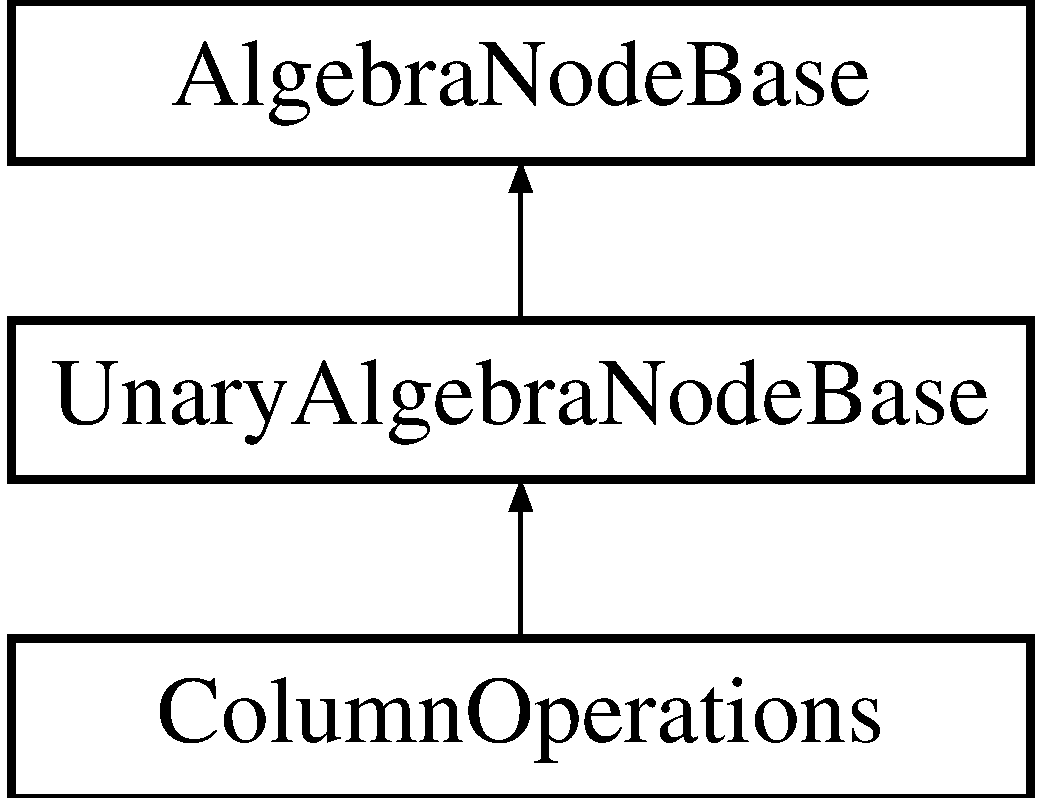
\includegraphics[height=3.000000cm]{class_column_operations}
\end{center}
\end{figure}
\subsection*{Public Member Functions}
\begin{DoxyCompactItemize}
\item 
\hypertarget{class_column_operations_a3d2c43e31201238da369906ef863c959}{{\bfseries Column\+Operations} (D\+O\+M\+Element $\ast$element)}\label{class_column_operations_a3d2c43e31201238da369906ef863c959}

\item 
\hypertarget{class_column_operations_aa33d719aa0407f588cd4ddc2d54368a6}{void {\bfseries accept} (\hyperlink{class_algebra_visitor}{Algebra\+Visitor} \&v)}\label{class_column_operations_aa33d719aa0407f588cd4ddc2d54368a6}

\end{DoxyCompactItemize}
\subsection*{Public Attributes}
\begin{DoxyCompactItemize}
\item 
\hypertarget{class_column_operations_a31aab19a9f8b104f772c111e920dd682}{std\+::vector$<$ \hyperlink{class_column_operation}{Column\+Operation} $>$ {\bfseries operations}}\label{class_column_operations_a31aab19a9f8b104f772c111e920dd682}

\end{DoxyCompactItemize}


The documentation for this class was generated from the following files\+:\begin{DoxyCompactItemize}
\item 
C\+:/\+Users/\+Marcel/\+Documents/\+Visual Studio 2012/\+Projects/\+Relational\+Query\+Evaluator/\+Relational\+Query\+Evaluator/Algebra.\+h\item 
C\+:/\+Users/\+Marcel/\+Documents/\+Visual Studio 2012/\+Projects/\+Relational\+Query\+Evaluator/\+Relational\+Query\+Evaluator/Algebra.\+cpp\end{DoxyCompactItemize}

\hypertarget{class_columns_operations_operator}{\section{Columns\+Operations\+Operator Class Reference}
\label{class_columns_operations_operator}\index{Columns\+Operations\+Operator@{Columns\+Operations\+Operator}}
}
Inheritance diagram for Columns\+Operations\+Operator\+:\begin{figure}[H]
\begin{center}
\leavevmode
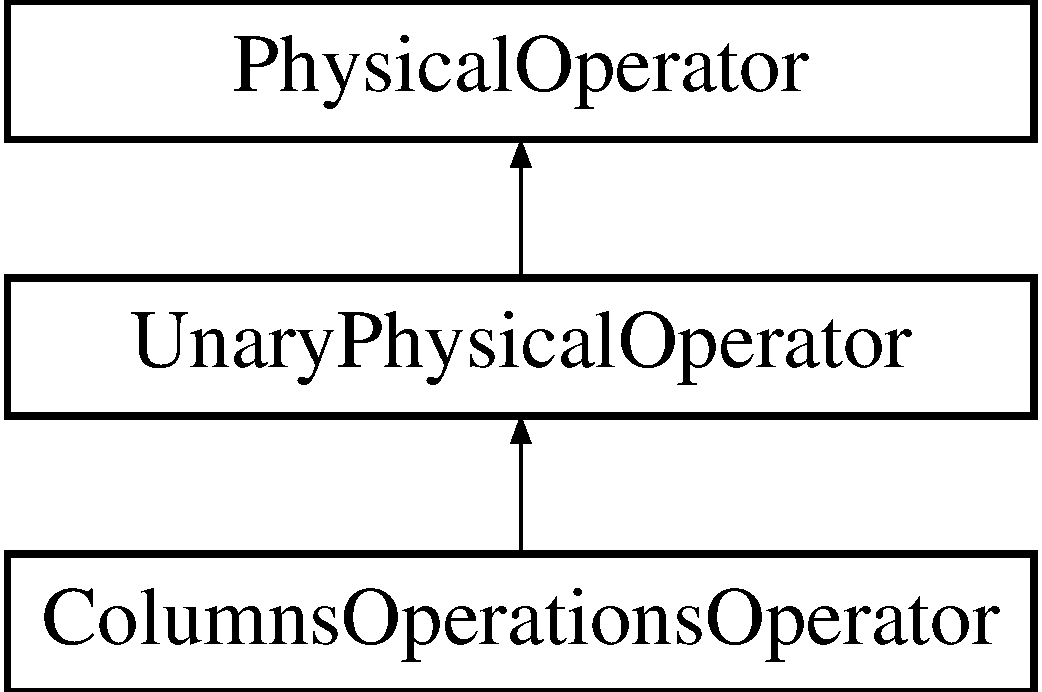
\includegraphics[height=3.000000cm]{class_columns_operations_operator}
\end{center}
\end{figure}
\subsection*{Public Member Functions}
\begin{DoxyCompactItemize}
\item 
\hypertarget{class_columns_operations_operator_a19cb4f96df418cd1a94a4906da06e20d}{{\bfseries Columns\+Operations\+Operator} (const std\+::vector$<$ \hyperlink{class_column_operation}{Column\+Operation} $>$ \&operations)}\label{class_columns_operations_operator_a19cb4f96df418cd1a94a4906da06e20d}

\item 
\hypertarget{class_columns_operations_operator_a5d40e806cb9dbd2969b45c28d7729f76}{void {\bfseries accept} (\hyperlink{class_physical_operator_visitor}{Physical\+Operator\+Visitor} \&v)}\label{class_columns_operations_operator_a5d40e806cb9dbd2969b45c28d7729f76}

\end{DoxyCompactItemize}
\subsection*{Public Attributes}
\begin{DoxyCompactItemize}
\item 
\hypertarget{class_columns_operations_operator_ae2384aeda586f5c60013dbe0cb5a3030}{std\+::vector$<$ \hyperlink{class_column_operation}{Column\+Operation} $>$ {\bfseries operations}}\label{class_columns_operations_operator_ae2384aeda586f5c60013dbe0cb5a3030}

\end{DoxyCompactItemize}


The documentation for this class was generated from the following files\+:\begin{DoxyCompactItemize}
\item 
C\+:/\+Users/\+Marcel/\+Documents/\+Visual Studio 2012/\+Projects/\+Relational\+Query\+Evaluator/\+Relational\+Query\+Evaluator/Physical\+Operator.\+h\item 
C\+:/\+Users/\+Marcel/\+Documents/\+Visual Studio 2012/\+Projects/\+Relational\+Query\+Evaluator/\+Relational\+Query\+Evaluator/Physical\+Operator.\+cpp\end{DoxyCompactItemize}

\hypertarget{class_condition_info}{\section{Condition\+Info Class Reference}
\label{class_condition_info}\index{Condition\+Info@{Condition\+Info}}
}


{\ttfamily \#include $<$Algebra\+Visitors.\+h$>$}

\subsection*{Public Attributes}
\begin{DoxyCompactItemize}
\item 
std\+::shared\+\_\+ptr$<$ \hyperlink{class_expression}{Expression} $>$ \hyperlink{class_condition_info_a57923bd70f56a79ca3ae8d09bb14f550}{condition}
\item 
std\+::set$<$ int $>$ \hyperlink{class_condition_info_ab800ad40c4040827cd93acc048863213}{inputs}
\item 
Condition\+Type \hyperlink{class_condition_info_a8ceacc67eb6d52679a9541764fd8b7d6}{type}
\end{DoxyCompactItemize}


\subsection{Detailed Description}
Stores information about condition, its columns and condition type. 

\subsection{Member Data Documentation}
\hypertarget{class_condition_info_a57923bd70f56a79ca3ae8d09bb14f550}{\index{Condition\+Info@{Condition\+Info}!condition@{condition}}
\index{condition@{condition}!Condition\+Info@{Condition\+Info}}
\subsubsection[{condition}]{\setlength{\rightskip}{0pt plus 5cm}std\+::shared\+\_\+ptr$<${\bf Expression}$>$ Condition\+Info\+::condition}}\label{class_condition_info_a57923bd70f56a79ca3ae8d09bb14f550}
Given condition. \hypertarget{class_condition_info_ab800ad40c4040827cd93acc048863213}{\index{Condition\+Info@{Condition\+Info}!inputs@{inputs}}
\index{inputs@{inputs}!Condition\+Info@{Condition\+Info}}
\subsubsection[{inputs}]{\setlength{\rightskip}{0pt plus 5cm}std\+::set$<$int$>$ Condition\+Info\+::inputs}}\label{class_condition_info_ab800ad40c4040827cd93acc048863213}
Set of column identifiers. \hypertarget{class_condition_info_a8ceacc67eb6d52679a9541764fd8b7d6}{\index{Condition\+Info@{Condition\+Info}!type@{type}}
\index{type@{type}!Condition\+Info@{Condition\+Info}}
\subsubsection[{type}]{\setlength{\rightskip}{0pt plus 5cm}Condition\+Type Condition\+Info\+::type}}\label{class_condition_info_a8ceacc67eb6d52679a9541764fd8b7d6}
Condition type. 

The documentation for this class was generated from the following file\+:\begin{DoxyCompactItemize}
\item 
C\+:/\+Users/\+Marcel/\+Documents/\+Visual Studio 2012/\+Projects/\+Relational\+Query\+Evaluator/\+Relational\+Query\+Evaluator/Algebra\+Visitors.\+h\end{DoxyCompactItemize}

\hypertarget{class_constant}{\section{Constant Class Reference}
\label{class_constant}\index{Constant@{Constant}}
}


{\ttfamily \#include $<$Expressions.\+h$>$}

Inheritance diagram for Constant\+:\begin{figure}[H]
\begin{center}
\leavevmode
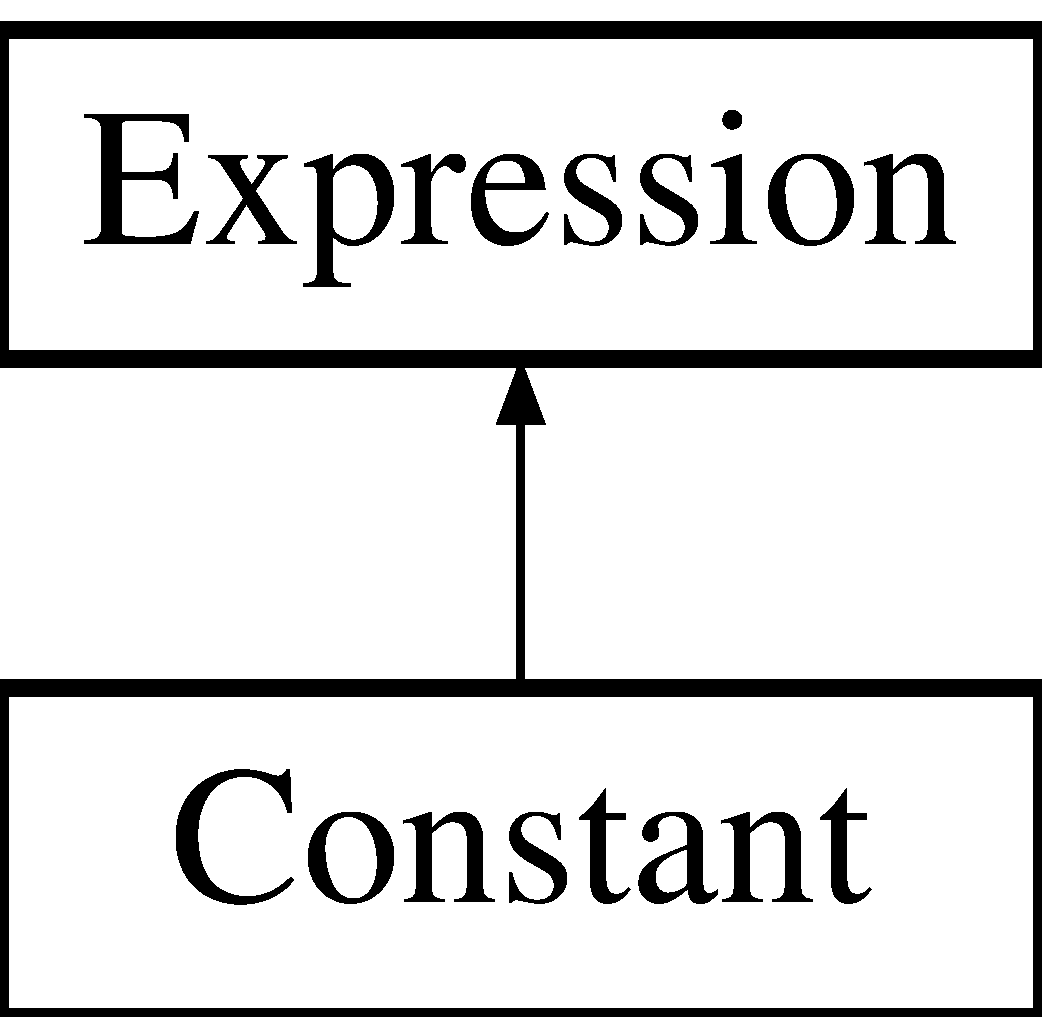
\includegraphics[height=2.000000cm]{class_constant}
\end{center}
\end{figure}
\subsection*{Public Member Functions}
\begin{DoxyCompactItemize}
\item 
\hyperlink{class_constant_a23cf0950dbddde0872f58ad5a501ff3a}{Constant} (D\+O\+M\+Element $\ast$node)
\item 
void \hyperlink{class_constant_ae30bbf2455dd5d616291e106749ec1ae}{accept} (\hyperlink{class_expression_visitor_base}{Expression\+Visitor\+Base} \&v)
\item 
void \hyperlink{class_constant_acb214c5b00f30970ad525eb6b2f3e04d}{replace\+Child} (\hyperlink{class_expression}{Expression} $\ast$old\+Child, std\+::shared\+\_\+ptr$<$ \hyperlink{class_expression}{Expression} $>$ new\+Child)
\end{DoxyCompactItemize}
\subsection*{Public Attributes}
\begin{DoxyCompactItemize}
\item 
std\+::string \hyperlink{class_constant_a97bcf14e26810def51c57ae446d69e06}{value}
\item 
std\+::string \hyperlink{class_constant_aa730d17869971537ca16ffd658b9d4e0}{type}
\end{DoxyCompactItemize}
\subsection*{Additional Inherited Members}


\subsection{Detailed Description}
Represents constant expression. It doesnt have any child expressions. 

\subsection{Constructor \& Destructor Documentation}
\hypertarget{class_constant_a23cf0950dbddde0872f58ad5a501ff3a}{\index{Constant@{Constant}!Constant@{Constant}}
\index{Constant@{Constant}!Constant@{Constant}}
\subsubsection[{Constant}]{\setlength{\rightskip}{0pt plus 5cm}Constant\+::\+Constant (
\begin{DoxyParamCaption}
\item[{D\+O\+M\+Element $\ast$}]{node}
\end{DoxyParamCaption}
)}}\label{class_constant_a23cf0950dbddde0872f58ad5a501ff3a}
Creates new instance of \hyperlink{class_constant}{Constant}. 
\begin{DoxyParams}{Parameters}
{\em node} & -\/ element containing infromation about constant. \\
\hline
\end{DoxyParams}


\subsection{Member Function Documentation}
\hypertarget{class_constant_ae30bbf2455dd5d616291e106749ec1ae}{\index{Constant@{Constant}!accept@{accept}}
\index{accept@{accept}!Constant@{Constant}}
\subsubsection[{accept}]{\setlength{\rightskip}{0pt plus 5cm}void Constant\+::accept (
\begin{DoxyParamCaption}
\item[{{\bf Expression\+Visitor\+Base} \&}]{v}
\end{DoxyParamCaption}
)\hspace{0.3cm}{\ttfamily [virtual]}}}\label{class_constant_ae30bbf2455dd5d616291e106749ec1ae}
Method for calling visit\mbox{[}node\mbox{]} on given Expression\+Visitor 
\begin{DoxyParams}{Parameters}
{\em v} & Expression\+Visitor, on which to call visit function \\
\hline
\end{DoxyParams}


Implements \hyperlink{class_expression_ae2e6c802668a6329658b7c982f9c7b33}{Expression}.

\hypertarget{class_constant_acb214c5b00f30970ad525eb6b2f3e04d}{\index{Constant@{Constant}!replace\+Child@{replace\+Child}}
\index{replace\+Child@{replace\+Child}!Constant@{Constant}}
\subsubsection[{replace\+Child}]{\setlength{\rightskip}{0pt plus 5cm}void Constant\+::replace\+Child (
\begin{DoxyParamCaption}
\item[{{\bf Expression} $\ast$}]{old\+Child, }
\item[{std\+::shared\+\_\+ptr$<$ {\bf Expression} $>$}]{new\+Child}
\end{DoxyParamCaption}
)\hspace{0.3cm}{\ttfamily [virtual]}}}\label{class_constant_acb214c5b00f30970ad525eb6b2f3e04d}
Replaces child from this class with new expression tree. 
\begin{DoxyParams}{Parameters}
{\em old\+Child} & -\/ child to replace \\
\hline
{\em new\+Child} & -\/ child to be replaced \\
\hline
\end{DoxyParams}


Implements \hyperlink{class_expression_a77ac16bbb0df93de8a7711b2f7de889f}{Expression}.



\subsection{Member Data Documentation}
\hypertarget{class_constant_aa730d17869971537ca16ffd658b9d4e0}{\index{Constant@{Constant}!type@{type}}
\index{type@{type}!Constant@{Constant}}
\subsubsection[{type}]{\setlength{\rightskip}{0pt plus 5cm}std\+::string Constant\+::type}}\label{class_constant_aa730d17869971537ca16ffd658b9d4e0}
Stores constant type. \hypertarget{class_constant_a97bcf14e26810def51c57ae446d69e06}{\index{Constant@{Constant}!value@{value}}
\index{value@{value}!Constant@{Constant}}
\subsubsection[{value}]{\setlength{\rightskip}{0pt plus 5cm}std\+::string Constant\+::value}}\label{class_constant_a97bcf14e26810def51c57ae446d69e06}
Stores constant value. 

The documentation for this class was generated from the following files\+:\begin{DoxyCompactItemize}
\item 
C\+:/\+Users/\+Marcel/\+Documents/\+Visual Studio 2012/\+Projects/\+Relational\+Query\+Evaluator/\+Relational\+Query\+Evaluator/Expressions.\+h\item 
C\+:/\+Users/\+Marcel/\+Documents/\+Visual Studio 2012/\+Projects/\+Relational\+Query\+Evaluator/\+Relational\+Query\+Evaluator/Expressions.\+cpp\end{DoxyCompactItemize}

\hypertarget{class_cross_join}{\section{Cross\+Join Class Reference}
\label{class_cross_join}\index{Cross\+Join@{Cross\+Join}}
}


{\ttfamily \#include $<$Physical\+Operator.\+h$>$}

Inheritance diagram for Cross\+Join\+:\begin{figure}[H]
\begin{center}
\leavevmode
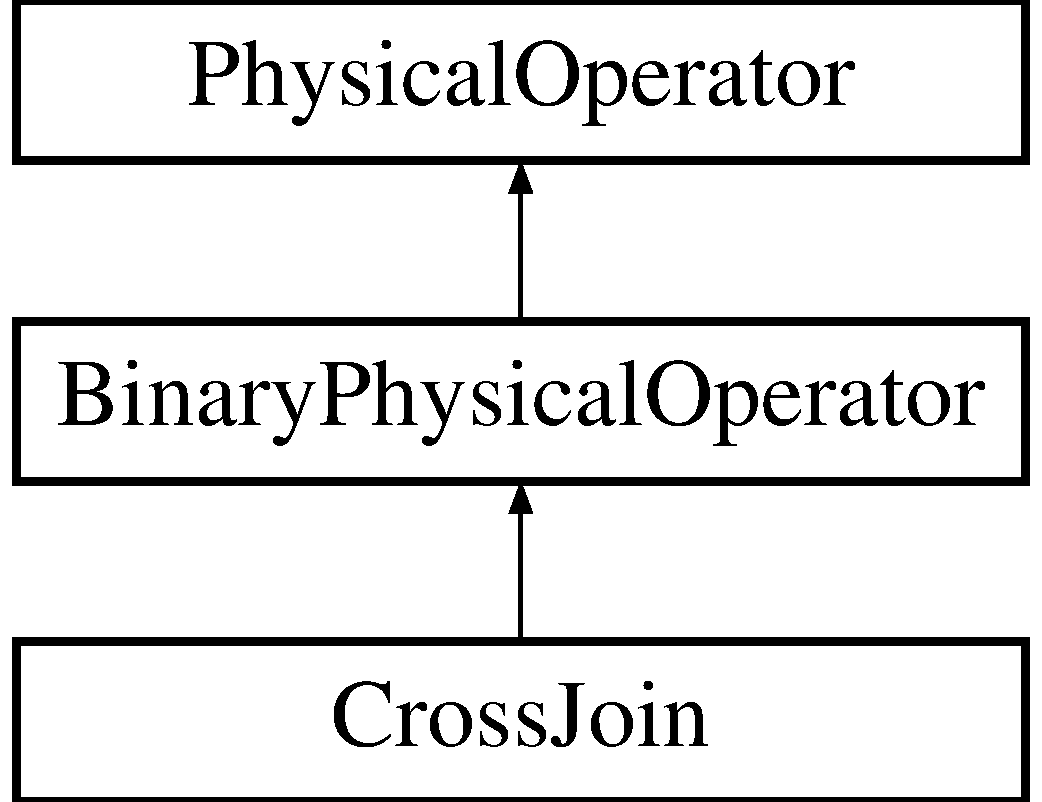
\includegraphics[height=3.000000cm]{class_cross_join}
\end{center}
\end{figure}
\subsection*{Public Member Functions}
\begin{DoxyCompactItemize}
\item 
void \hyperlink{class_cross_join_a92a1a35e3940c6c8bdaa6722d476c5db}{accept} (\hyperlink{class_physical_operator_visitor}{Physical\+Operator\+Visitor} \&v)
\end{DoxyCompactItemize}
\subsection*{Additional Inherited Members}


\subsection{Detailed Description}
Represents physical cross join operator. Operator computes Cartesian product from given inputs. 

\subsection{Member Function Documentation}
\hypertarget{class_cross_join_a92a1a35e3940c6c8bdaa6722d476c5db}{\index{Cross\+Join@{Cross\+Join}!accept@{accept}}
\index{accept@{accept}!Cross\+Join@{Cross\+Join}}
\subsubsection[{accept}]{\setlength{\rightskip}{0pt plus 5cm}void Cross\+Join\+::accept (
\begin{DoxyParamCaption}
\item[{{\bf Physical\+Operator\+Visitor} \&}]{v}
\end{DoxyParamCaption}
)\hspace{0.3cm}{\ttfamily [virtual]}}}\label{class_cross_join_a92a1a35e3940c6c8bdaa6722d476c5db}
Method for calling visit\mbox{[}node\mbox{]} on given \hyperlink{class_physical_operator_visitor}{Physical\+Operator\+Visitor}. 
\begin{DoxyParams}{Parameters}
{\em v} & \hyperlink{class_physical_operator_visitor}{Physical\+Operator\+Visitor}, on which to call function. \\
\hline
\end{DoxyParams}


Implements \hyperlink{class_binary_physical_operator_a29ec622920006cb5428bf2c259918347}{Binary\+Physical\+Operator}.



The documentation for this class was generated from the following files\+:\begin{DoxyCompactItemize}
\item 
C\+:/\+Users/\+Marcel/\+Documents/\+Visual Studio 2012/\+Projects/\+Relational\+Query\+Evaluator/\+Relational\+Query\+Evaluator/Physical\+Operator.\+h\item 
C\+:/\+Users/\+Marcel/\+Documents/\+Visual Studio 2012/\+Projects/\+Relational\+Query\+Evaluator/\+Relational\+Query\+Evaluator/Physical\+Operator.\+cpp\end{DoxyCompactItemize}

\hypertarget{class_d_o_m_parser}{\section{D\+O\+M\+Parser Class Reference}
\label{class_d_o_m_parser}\index{D\+O\+M\+Parser@{D\+O\+M\+Parser}}
}
Inheritance diagram for D\+O\+M\+Parser\+:\begin{figure}[H]
\begin{center}
\leavevmode
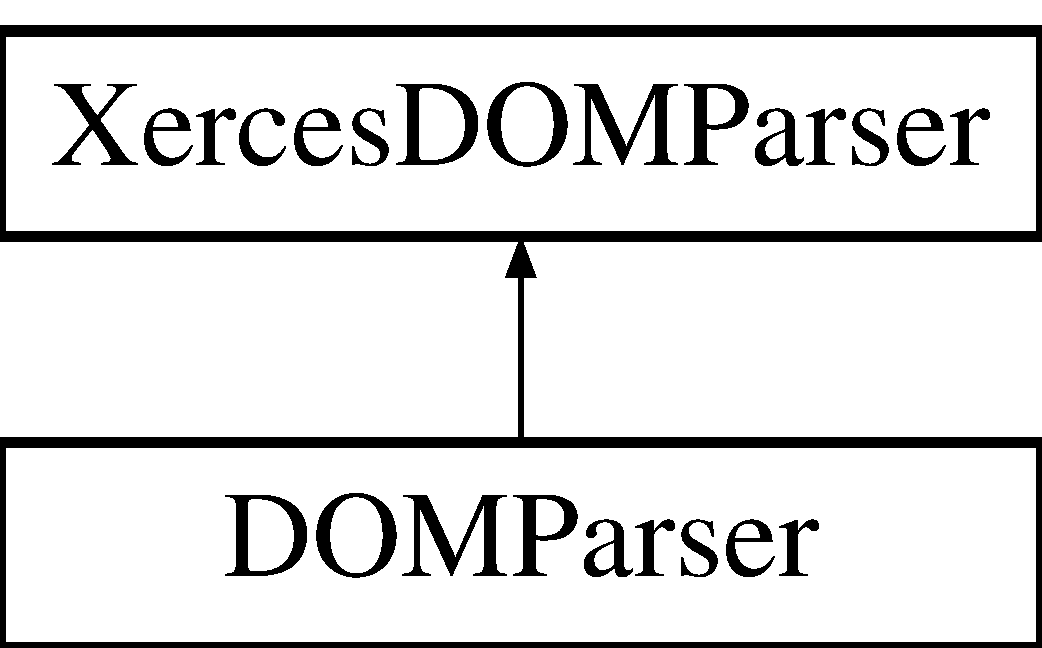
\includegraphics[height=2.000000cm]{class_d_o_m_parser}
\end{center}
\end{figure}
\subsection*{Public Member Functions}
\begin{DoxyCompactItemize}
\item 
\hypertarget{class_d_o_m_parser_ad1d0d1baa8de927488a0a528d6ef0298}{void {\bfseries start\+Element} (const X\+M\+L\+Element\+Decl \&elem\+Decl, const unsigned int url\+Id, const X\+M\+L\+Ch $\ast$const elem\+Prefix, const Ref\+Vector\+Of$<$ X\+M\+L\+Attr $>$ \&attr\+List, const X\+M\+L\+Size\+\_\+t attr\+Count, const bool is\+Empty, const bool is\+Root)}\label{class_d_o_m_parser_ad1d0d1baa8de927488a0a528d6ef0298}

\end{DoxyCompactItemize}


The documentation for this class was generated from the following file\+:\begin{DoxyCompactItemize}
\item 
C\+:/\+Users/\+Marcel/\+Documents/\+Visual Studio 2012/\+Projects/\+Relational\+Query\+Evaluator/\+Relational\+Query\+Evaluator/Xml\+Handler.\+h\end{DoxyCompactItemize}

\hypertarget{class_expression}{\section{Expression Class Reference}
\label{class_expression}\index{Expression@{Expression}}
}


{\ttfamily \#include $<$Expressions.\+h$>$}

Inheritance diagram for Expression\+:\begin{figure}[H]
\begin{center}
\leavevmode
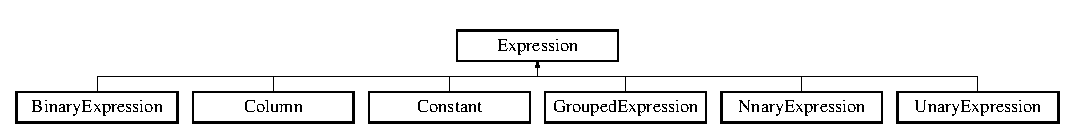
\includegraphics[height=1.424936cm]{class_expression}
\end{center}
\end{figure}
\subsection*{Public Member Functions}
\begin{DoxyCompactItemize}
\item 
virtual void \hyperlink{class_expression_ae2e6c802668a6329658b7c982f9c7b33}{accept} (\hyperlink{class_expression_visitor_base}{Expression\+Visitor\+Base} \&v)=0
\item 
virtual void \hyperlink{class_expression_a77ac16bbb0df93de8a7711b2f7de889f}{replace\+Child} (\hyperlink{class_expression}{Expression} $\ast$old\+Child, std\+::shared\+\_\+ptr$<$ \hyperlink{class_expression}{Expression} $>$ new\+Child)=0
\end{DoxyCompactItemize}
\subsection*{Static Public Member Functions}
\begin{DoxyCompactItemize}
\item 
static \hyperlink{class_expression}{Expression} $\ast$ \hyperlink{class_expression_ae1968c4b3272019059f9a51e40d65c41}{construct\+Children} (D\+O\+M\+Element $\ast$node)
\end{DoxyCompactItemize}
\subsection*{Public Attributes}
\begin{DoxyCompactItemize}
\item 
\hyperlink{class_expression}{Expression} $\ast$ \hyperlink{class_expression_a36284ba467eae6aa796985ed909a6958}{parent}
\end{DoxyCompactItemize}


\subsection{Detailed Description}
Base class for expression in expressionn tree. \hyperlink{class_expression}{Expression} trees are used in algebra nodes like selection, join, antijoin or column operations. 

\subsection{Member Function Documentation}
\hypertarget{class_expression_ae2e6c802668a6329658b7c982f9c7b33}{\index{Expression@{Expression}!accept@{accept}}
\index{accept@{accept}!Expression@{Expression}}
\subsubsection[{accept}]{\setlength{\rightskip}{0pt plus 5cm}virtual void Expression\+::accept (
\begin{DoxyParamCaption}
\item[{{\bf Expression\+Visitor\+Base} \&}]{v}
\end{DoxyParamCaption}
)\hspace{0.3cm}{\ttfamily [pure virtual]}}}\label{class_expression_ae2e6c802668a6329658b7c982f9c7b33}
Method for calling visit\mbox{[}node\mbox{]} on given Expression\+Visitor 
\begin{DoxyParams}{Parameters}
{\em v} & Expression\+Visitor, on which to call visit function \\
\hline
\end{DoxyParams}


Implemented in \hyperlink{class_grouped_expression_a67963e289263b9c2cbf03edad83401b7}{Grouped\+Expression}, \hyperlink{class_column_a6e925985b1e87ed92795d318c52e5470}{Column}, \hyperlink{class_constant_ae30bbf2455dd5d616291e106749ec1ae}{Constant}, \hyperlink{class_nnary_expression_a5934f3925e13888b3241f6b269d5ee44}{Nnary\+Expression}, \hyperlink{class_binary_expression_a12ea9a0735a8809b01059988b6466d7c}{Binary\+Expression}, and \hyperlink{class_unary_expression_a34d44f441b84b899b832cbd46b4b7821}{Unary\+Expression}.

\hypertarget{class_expression_ae1968c4b3272019059f9a51e40d65c41}{\index{Expression@{Expression}!construct\+Children@{construct\+Children}}
\index{construct\+Children@{construct\+Children}!Expression@{Expression}}
\subsubsection[{construct\+Children}]{\setlength{\rightskip}{0pt plus 5cm}{\bf Expression} $\ast$ Expression\+::construct\+Children (
\begin{DoxyParamCaption}
\item[{D\+O\+M\+Element $\ast$}]{node}
\end{DoxyParamCaption}
)\hspace{0.3cm}{\ttfamily [static]}}}\label{class_expression_ae1968c4b3272019059f9a51e40d65c41}
Helper function for choosing which node to conctruct from element. 
\begin{DoxyParams}{Parameters}
{\em node} & -\/ element containing information expression \\
\hline
\end{DoxyParams}
\hypertarget{class_expression_a77ac16bbb0df93de8a7711b2f7de889f}{\index{Expression@{Expression}!replace\+Child@{replace\+Child}}
\index{replace\+Child@{replace\+Child}!Expression@{Expression}}
\subsubsection[{replace\+Child}]{\setlength{\rightskip}{0pt plus 5cm}virtual void Expression\+::replace\+Child (
\begin{DoxyParamCaption}
\item[{{\bf Expression} $\ast$}]{old\+Child, }
\item[{std\+::shared\+\_\+ptr$<$ {\bf Expression} $>$}]{new\+Child}
\end{DoxyParamCaption}
)\hspace{0.3cm}{\ttfamily [pure virtual]}}}\label{class_expression_a77ac16bbb0df93de8a7711b2f7de889f}
Replaces child from this class with new expression tree. 
\begin{DoxyParams}{Parameters}
{\em old\+Child} & -\/ child to replace \\
\hline
{\em new\+Child} & -\/ child to be replaced \\
\hline
\end{DoxyParams}


Implemented in \hyperlink{class_grouped_expression_af1cb9044417df12361b6335962b3bc6c}{Grouped\+Expression}, \hyperlink{class_column_af1571fb51f887aeb1dcf7ff44382a72b}{Column}, \hyperlink{class_constant_acb214c5b00f30970ad525eb6b2f3e04d}{Constant}, \hyperlink{class_nnary_expression_a1161a6f8776c4cc946d769e4526339a2}{Nnary\+Expression}, \hyperlink{class_binary_expression_a7ff9236432aef24bca655ab45cf475f2}{Binary\+Expression}, and \hyperlink{class_unary_expression_ae1a0cfc5fbae6d401c28e8a3158121a3}{Unary\+Expression}.



\subsection{Member Data Documentation}
\hypertarget{class_expression_a36284ba467eae6aa796985ed909a6958}{\index{Expression@{Expression}!parent@{parent}}
\index{parent@{parent}!Expression@{Expression}}
\subsubsection[{parent}]{\setlength{\rightskip}{0pt plus 5cm}{\bf Expression}$\ast$ Expression\+::parent}}\label{class_expression_a36284ba467eae6aa796985ed909a6958}
Stores pointer on the parent in expression tree. 

The documentation for this class was generated from the following files\+:\begin{DoxyCompactItemize}
\item 
C\+:/\+Users/\+Marcel/\+Documents/\+Visual Studio 2012/\+Projects/\+Relational\+Query\+Evaluator/\+Relational\+Query\+Evaluator/Expressions.\+h\item 
C\+:/\+Users/\+Marcel/\+Documents/\+Visual Studio 2012/\+Projects/\+Relational\+Query\+Evaluator/\+Relational\+Query\+Evaluator/Expressions.\+cpp\end{DoxyCompactItemize}

\hypertarget{class_expression_visitor_base}{\section{Expression\+Visitor\+Base Class Reference}
\label{class_expression_visitor_base}\index{Expression\+Visitor\+Base@{Expression\+Visitor\+Base}}
}
Inheritance diagram for Expression\+Visitor\+Base\+:\begin{figure}[H]
\begin{center}
\leavevmode
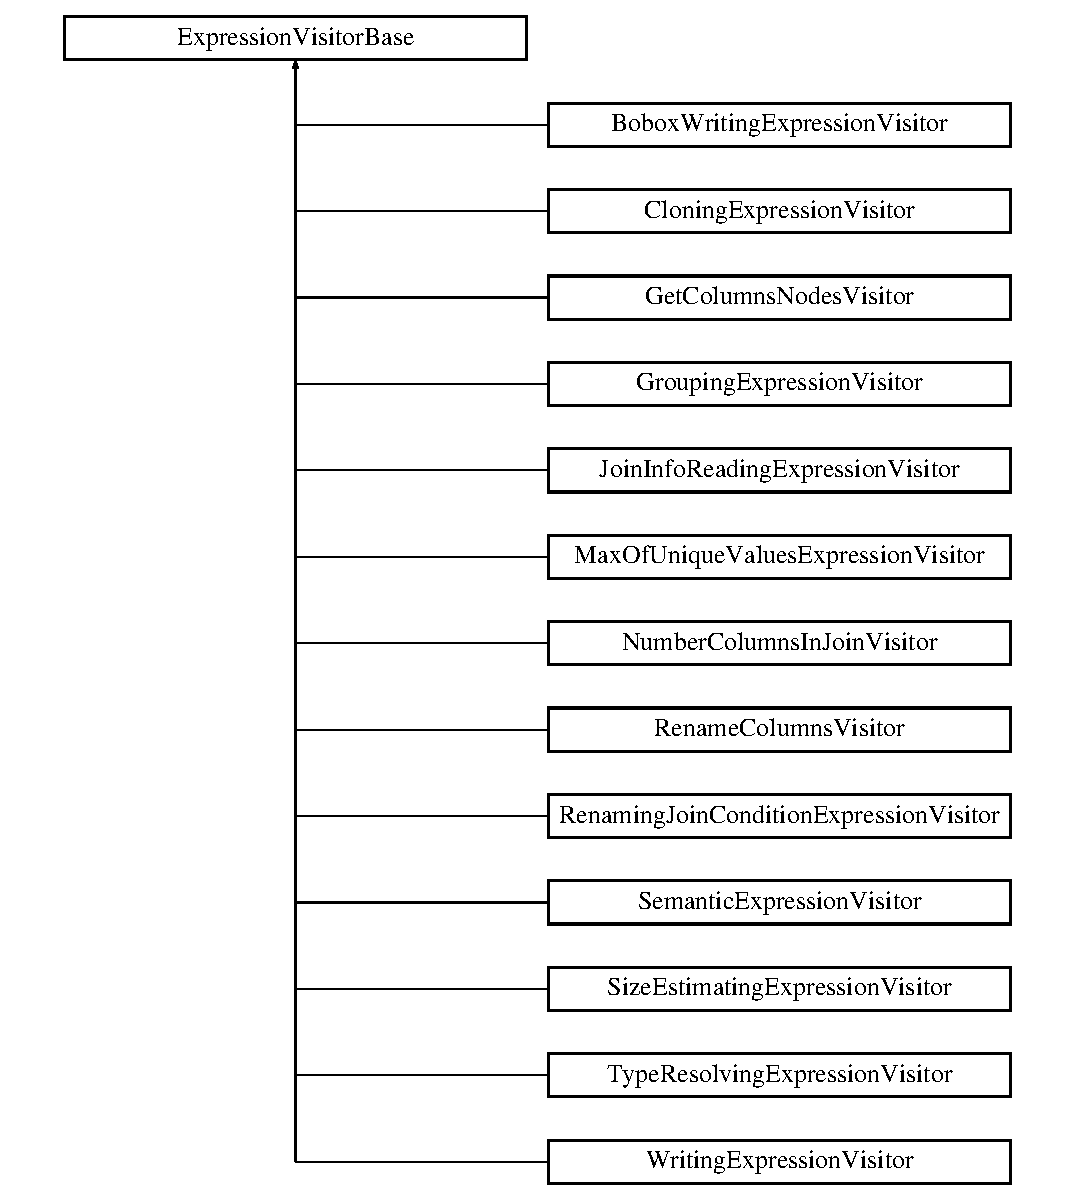
\includegraphics[height=12.000000cm]{class_expression_visitor_base}
\end{center}
\end{figure}
\subsection*{Public Member Functions}
\begin{DoxyCompactItemize}
\item 
\hypertarget{class_expression_visitor_base_aeda112c1084f60e161b9b3c1a9cf0f5b}{virtual void {\bfseries visit\+Expression} (\hyperlink{class_expression}{Expression} $\ast$expression)}\label{class_expression_visitor_base_aeda112c1084f60e161b9b3c1a9cf0f5b}

\item 
\hypertarget{class_expression_visitor_base_a9750397f5588263509a28ca9f17e8bc4}{virtual void {\bfseries visit\+Unary\+Expression} (\hyperlink{class_unary_expression}{Unary\+Expression} $\ast$expression)}\label{class_expression_visitor_base_a9750397f5588263509a28ca9f17e8bc4}

\item 
\hypertarget{class_expression_visitor_base_aebbbbe9a1cecabe4c4804bf1ef82a9f9}{virtual void {\bfseries visit\+Binary\+Expression} (\hyperlink{class_binary_expression}{Binary\+Expression} $\ast$expression)}\label{class_expression_visitor_base_aebbbbe9a1cecabe4c4804bf1ef82a9f9}

\item 
\hypertarget{class_expression_visitor_base_a010c5ba36b255c8576a2b36aaf9692d8}{virtual void {\bfseries visit\+Nnary\+Expression} (\hyperlink{class_nnary_expression}{Nnary\+Expression} $\ast$expression)}\label{class_expression_visitor_base_a010c5ba36b255c8576a2b36aaf9692d8}

\item 
\hypertarget{class_expression_visitor_base_a64921e6a6a4945faf693e9ef8d6310a4}{virtual void {\bfseries visit\+Constant} (\hyperlink{class_constant}{Constant} $\ast$expression)}\label{class_expression_visitor_base_a64921e6a6a4945faf693e9ef8d6310a4}

\item 
\hypertarget{class_expression_visitor_base_a1ac638b82248ff9e1582dbf520dc6ae4}{virtual void {\bfseries visit\+Column} (\hyperlink{class_column}{Column} $\ast$expression)}\label{class_expression_visitor_base_a1ac638b82248ff9e1582dbf520dc6ae4}

\item 
\hypertarget{class_expression_visitor_base_aec22a7bb476fc79e7997d188423514c0}{virtual void {\bfseries visit\+Grouped\+Expression} (\hyperlink{class_grouped_expression}{Grouped\+Expression} $\ast$expression)}\label{class_expression_visitor_base_aec22a7bb476fc79e7997d188423514c0}

\end{DoxyCompactItemize}


The documentation for this class was generated from the following files\+:\begin{DoxyCompactItemize}
\item 
C\+:/\+Users/\+Marcel/\+Documents/\+Visual Studio 2012/\+Projects/\+Relational\+Query\+Evaluator/\+Relational\+Query\+Evaluator/Expression\+Visitors.\+h\item 
C\+:/\+Users/\+Marcel/\+Documents/\+Visual Studio 2012/\+Projects/\+Relational\+Query\+Evaluator/\+Relational\+Query\+Evaluator/Expression\+Visitors.\+cpp\end{DoxyCompactItemize}

\hypertarget{class_filter}{\section{Filter Class Reference}
\label{class_filter}\index{Filter@{Filter}}
}


{\ttfamily \#include $<$Physical\+Operator.\+h$>$}

Inheritance diagram for Filter\+:\begin{figure}[H]
\begin{center}
\leavevmode
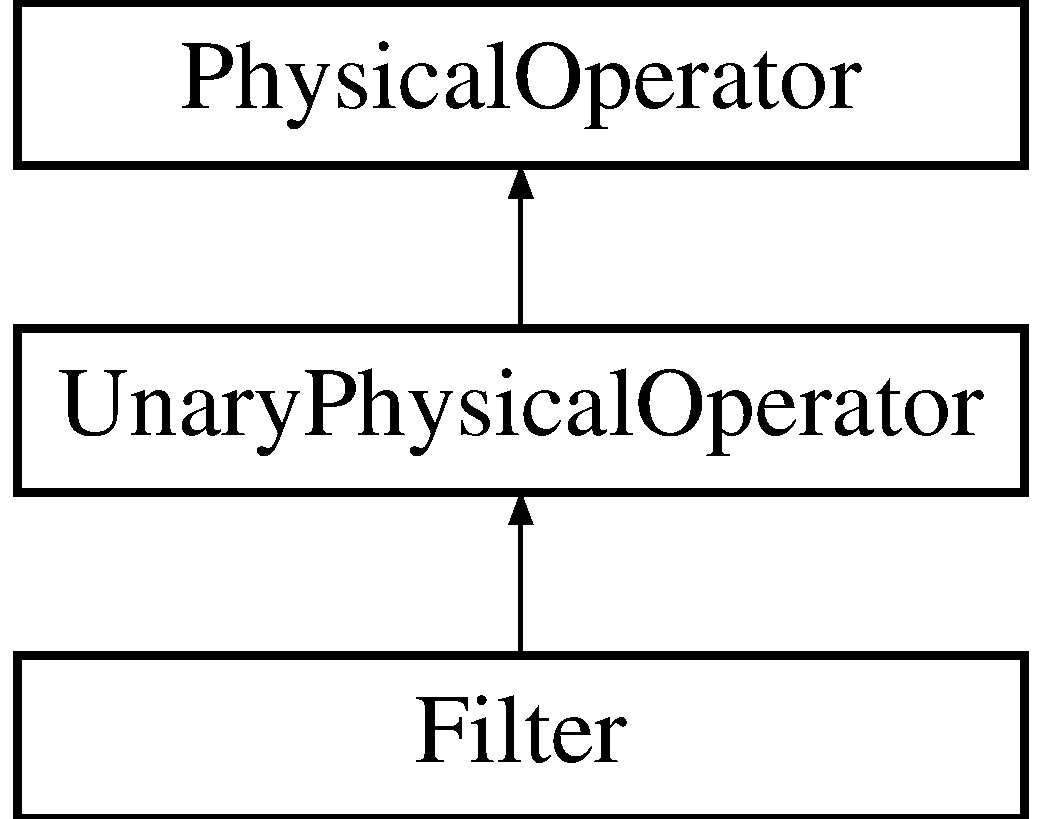
\includegraphics[height=3.000000cm]{class_filter}
\end{center}
\end{figure}
\subsection*{Public Member Functions}
\begin{DoxyCompactItemize}
\item 
\hyperlink{class_filter_a4e75723e5596f5b77b84a395c7453853}{Filter} (const std\+::shared\+\_\+ptr$<$ \hyperlink{class_expression}{Expression} $>$ \&\hyperlink{class_filter_acc551fc888d4b2e9bc36364a3877dbb8}{condition})
\item 
void \hyperlink{class_filter_a1df50e05d64ad3b2cc45d2f9e28127c4}{accept} (\hyperlink{class_physical_operator_visitor}{Physical\+Operator\+Visitor} \&v)
\end{DoxyCompactItemize}
\subsection*{Public Attributes}
\begin{DoxyCompactItemize}
\item 
std\+::shared\+\_\+ptr$<$ \hyperlink{class_expression}{Expression} $>$ \hyperlink{class_filter_acc551fc888d4b2e9bc36364a3877dbb8}{condition}
\end{DoxyCompactItemize}


\subsection{Detailed Description}
Class representing filter physical algorithm. Operator filters given rows and output only rows satisfying condition. Output doesn't have to be sorted same way as input. 

\subsection{Constructor \& Destructor Documentation}
\hypertarget{class_filter_a4e75723e5596f5b77b84a395c7453853}{\index{Filter@{Filter}!Filter@{Filter}}
\index{Filter@{Filter}!Filter@{Filter}}
\subsubsection[{Filter}]{\setlength{\rightskip}{0pt plus 5cm}Filter\+::\+Filter (
\begin{DoxyParamCaption}
\item[{const std\+::shared\+\_\+ptr$<$ {\bf Expression} $>$ \&}]{condition}
\end{DoxyParamCaption}
)}}\label{class_filter_a4e75723e5596f5b77b84a395c7453853}
Creates new instance of \hyperlink{class_filter}{Filter}. 
\begin{DoxyParams}{Parameters}
{\em condition} & -\/ filter condition. \\
\hline
\end{DoxyParams}


\subsection{Member Function Documentation}
\hypertarget{class_filter_a1df50e05d64ad3b2cc45d2f9e28127c4}{\index{Filter@{Filter}!accept@{accept}}
\index{accept@{accept}!Filter@{Filter}}
\subsubsection[{accept}]{\setlength{\rightskip}{0pt plus 5cm}void Filter\+::accept (
\begin{DoxyParamCaption}
\item[{{\bf Physical\+Operator\+Visitor} \&}]{v}
\end{DoxyParamCaption}
)\hspace{0.3cm}{\ttfamily [virtual]}}}\label{class_filter_a1df50e05d64ad3b2cc45d2f9e28127c4}
Method for calling visit\mbox{[}node\mbox{]} on given \hyperlink{class_physical_operator_visitor}{Physical\+Operator\+Visitor}. 
\begin{DoxyParams}{Parameters}
{\em v} & \hyperlink{class_physical_operator_visitor}{Physical\+Operator\+Visitor}, on which to call function. \\
\hline
\end{DoxyParams}


Implements \hyperlink{class_unary_physical_operator_a3b0160d380149213561ef2ba479dbf6a}{Unary\+Physical\+Operator}.



\subsection{Member Data Documentation}
\hypertarget{class_filter_acc551fc888d4b2e9bc36364a3877dbb8}{\index{Filter@{Filter}!condition@{condition}}
\index{condition@{condition}!Filter@{Filter}}
\subsubsection[{condition}]{\setlength{\rightskip}{0pt plus 5cm}std\+::shared\+\_\+ptr$<${\bf Expression}$>$ Filter\+::condition}}\label{class_filter_acc551fc888d4b2e9bc36364a3877dbb8}
Condition for filtering relation. 

The documentation for this class was generated from the following files\+:\begin{DoxyCompactItemize}
\item 
C\+:/\+Users/\+Marcel/\+Documents/\+Visual Studio 2012/\+Projects/\+Relational\+Query\+Evaluator/\+Relational\+Query\+Evaluator/Physical\+Operator.\+h\item 
C\+:/\+Users/\+Marcel/\+Documents/\+Visual Studio 2012/\+Projects/\+Relational\+Query\+Evaluator/\+Relational\+Query\+Evaluator/Physical\+Operator.\+cpp\end{DoxyCompactItemize}

\hypertarget{class_filter_keeping_order}{\section{Filter\+Keeping\+Order Class Reference}
\label{class_filter_keeping_order}\index{Filter\+Keeping\+Order@{Filter\+Keeping\+Order}}
}
Inheritance diagram for Filter\+Keeping\+Order\+:\begin{figure}[H]
\begin{center}
\leavevmode
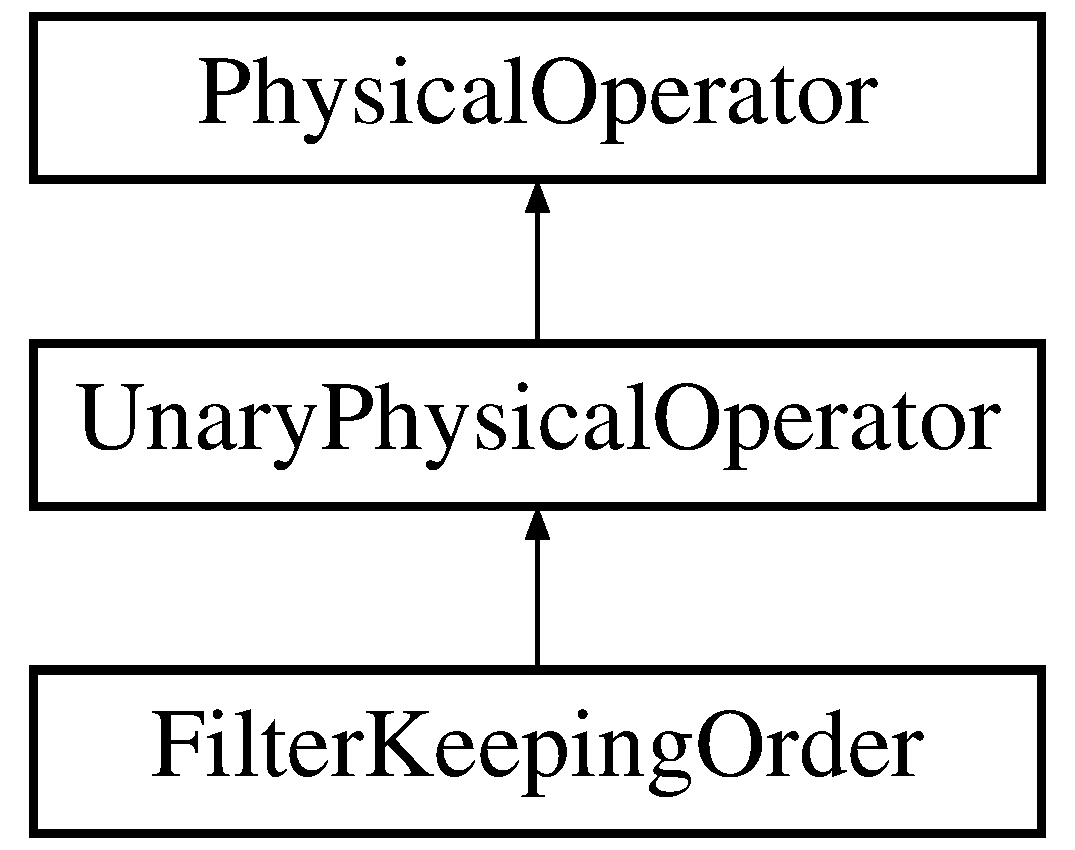
\includegraphics[height=3.000000cm]{class_filter_keeping_order}
\end{center}
\end{figure}
\subsection*{Public Member Functions}
\begin{DoxyCompactItemize}
\item 
\hypertarget{class_filter_keeping_order_abc6e727ea1b121b18bfd537a5c736676}{{\bfseries Filter\+Keeping\+Order} (const std\+::shared\+\_\+ptr$<$ \hyperlink{class_expression}{Expression} $>$ \&condition)}\label{class_filter_keeping_order_abc6e727ea1b121b18bfd537a5c736676}

\item 
\hypertarget{class_filter_keeping_order_a3d970e81588d96ac0d6538c17a22144c}{void {\bfseries accept} (\hyperlink{class_physical_operator_visitor}{Physical\+Operator\+Visitor} \&v)}\label{class_filter_keeping_order_a3d970e81588d96ac0d6538c17a22144c}

\end{DoxyCompactItemize}
\subsection*{Public Attributes}
\begin{DoxyCompactItemize}
\item 
\hypertarget{class_filter_keeping_order_a9958c9755be1bcd46a9fa67116d07e67}{std\+::shared\+\_\+ptr$<$ \hyperlink{class_expression}{Expression} $>$ {\bfseries condition}}\label{class_filter_keeping_order_a9958c9755be1bcd46a9fa67116d07e67}

\end{DoxyCompactItemize}


The documentation for this class was generated from the following files\+:\begin{DoxyCompactItemize}
\item 
C\+:/\+Users/\+Marcel/\+Documents/\+Visual Studio 2012/\+Projects/\+Relational\+Query\+Evaluator/\+Relational\+Query\+Evaluator/Physical\+Operator.\+h\item 
C\+:/\+Users/\+Marcel/\+Documents/\+Visual Studio 2012/\+Projects/\+Relational\+Query\+Evaluator/\+Relational\+Query\+Evaluator/Physical\+Operator.\+cpp\end{DoxyCompactItemize}

\hypertarget{class_get_columns_nodes_visitor}{\section{Get\+Columns\+Nodes\+Visitor Class Reference}
\label{class_get_columns_nodes_visitor}\index{Get\+Columns\+Nodes\+Visitor@{Get\+Columns\+Nodes\+Visitor}}
}


{\ttfamily \#include $<$Expression\+Visitors.\+h$>$}

Inheritance diagram for Get\+Columns\+Nodes\+Visitor\+:\begin{figure}[H]
\begin{center}
\leavevmode
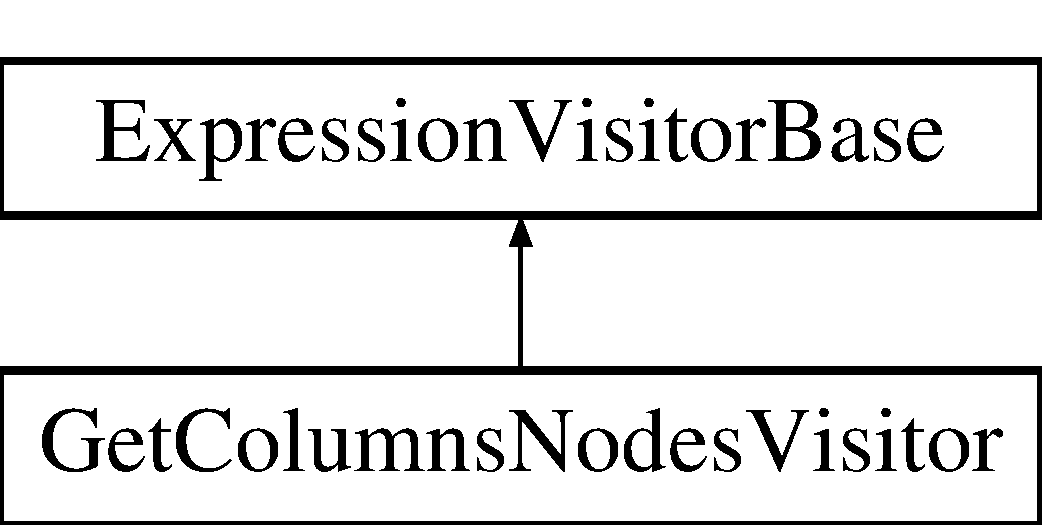
\includegraphics[height=2.000000cm]{class_get_columns_nodes_visitor}
\end{center}
\end{figure}
\subsection*{Public Member Functions}
\begin{DoxyCompactItemize}
\item 
void \hyperlink{class_get_columns_nodes_visitor_adcd58020e010392df2b543b6a4bbc46b}{visit\+Column} (\hyperlink{class_column}{Column} $\ast$expression)
\end{DoxyCompactItemize}
\subsection*{Public Attributes}
\begin{DoxyCompactItemize}
\item 
std\+::vector$<$ \hyperlink{class_column}{Column} $\ast$ $>$ \hyperlink{class_get_columns_nodes_visitor_ac68ee0c1090596d4e25a5dc5a478533b}{nodes}
\end{DoxyCompactItemize}


\subsection{Detailed Description}
Visitor, which stores pointer of every column into vector. This visitor doesn't change expression tree. 

\subsection{Member Function Documentation}
\hypertarget{class_get_columns_nodes_visitor_adcd58020e010392df2b543b6a4bbc46b}{\index{Get\+Columns\+Nodes\+Visitor@{Get\+Columns\+Nodes\+Visitor}!visit\+Column@{visit\+Column}}
\index{visit\+Column@{visit\+Column}!Get\+Columns\+Nodes\+Visitor@{Get\+Columns\+Nodes\+Visitor}}
\subsubsection[{visit\+Column}]{\setlength{\rightskip}{0pt plus 5cm}void Get\+Columns\+Nodes\+Visitor\+::visit\+Column (
\begin{DoxyParamCaption}
\item[{{\bf Column} $\ast$}]{expression}
\end{DoxyParamCaption}
)\hspace{0.3cm}{\ttfamily [virtual]}}}\label{class_get_columns_nodes_visitor_adcd58020e010392df2b543b6a4bbc46b}
Visits \hyperlink{class_column}{Column} element. 
\begin{DoxyParams}{Parameters}
{\em expression} & visited \hyperlink{class_column}{Column}. \\
\hline
\end{DoxyParams}


Reimplemented from \hyperlink{class_expression_visitor_base_a1ac638b82248ff9e1582dbf520dc6ae4}{Expression\+Visitor\+Base}.



\subsection{Member Data Documentation}
\hypertarget{class_get_columns_nodes_visitor_ac68ee0c1090596d4e25a5dc5a478533b}{\index{Get\+Columns\+Nodes\+Visitor@{Get\+Columns\+Nodes\+Visitor}!nodes@{nodes}}
\index{nodes@{nodes}!Get\+Columns\+Nodes\+Visitor@{Get\+Columns\+Nodes\+Visitor}}
\subsubsection[{nodes}]{\setlength{\rightskip}{0pt plus 5cm}std\+::vector$<${\bf Column} $\ast$$>$ Get\+Columns\+Nodes\+Visitor\+::nodes}}\label{class_get_columns_nodes_visitor_ac68ee0c1090596d4e25a5dc5a478533b}
Vector for saving column pointers. 

The documentation for this class was generated from the following files\+:\begin{DoxyCompactItemize}
\item 
C\+:/\+Users/\+Marcel/\+Documents/\+Visual Studio 2012/\+Projects/\+Relational\+Query\+Evaluator/\+Relational\+Query\+Evaluator/Expression\+Visitors.\+h\item 
C\+:/\+Users/\+Marcel/\+Documents/\+Visual Studio 2012/\+Projects/\+Relational\+Query\+Evaluator/\+Relational\+Query\+Evaluator/Expression\+Visitors.\+cpp\end{DoxyCompactItemize}

\hypertarget{class_graph_drawing_visitor}{\section{Graph\+Drawing\+Visitor Class Reference}
\label{class_graph_drawing_visitor}\index{Graph\+Drawing\+Visitor@{Graph\+Drawing\+Visitor}}
}


{\ttfamily \#include $<$Algebra\+Visitors.\+h$>$}

Inheritance diagram for Graph\+Drawing\+Visitor\+:\begin{figure}[H]
\begin{center}
\leavevmode
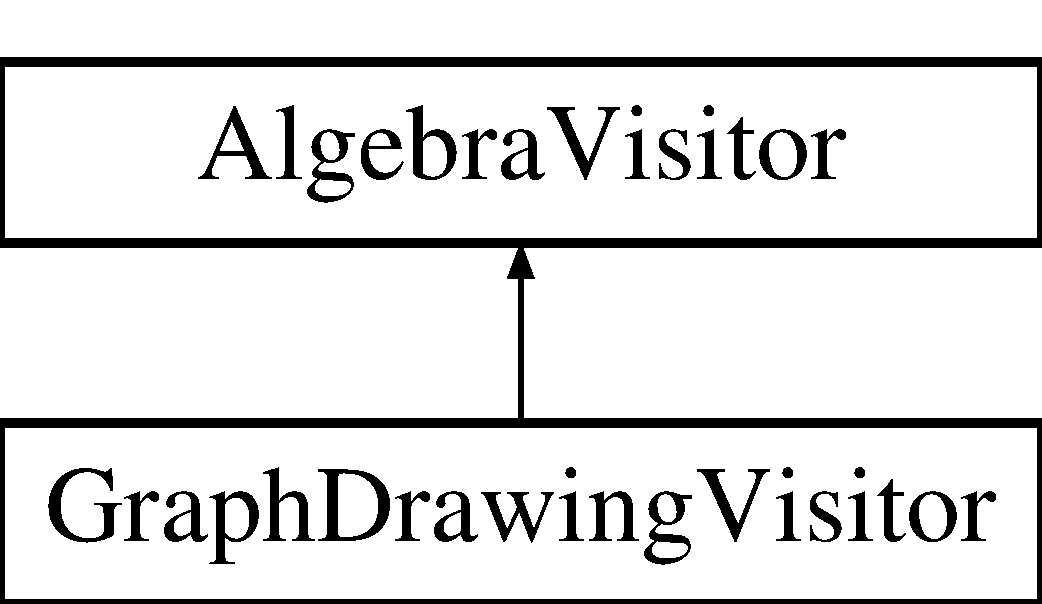
\includegraphics[height=2.000000cm]{class_graph_drawing_visitor}
\end{center}
\end{figure}
\subsection*{Public Member Functions}
\begin{DoxyCompactItemize}
\item 
\hyperlink{class_graph_drawing_visitor_a9d02755cb6c2b10984a573a28751ed8a}{Graph\+Drawing\+Visitor} ()
\item 
void \hyperlink{class_graph_drawing_visitor_a613ff576e75d1bf181b5786a3b7eec63}{generate\+Text} (std\+::string \&label, \hyperlink{class_unary_algebra_node_base}{Unary\+Algebra\+Node\+Base} $\ast$node)
\item 
void \hyperlink{class_graph_drawing_visitor_a4cd34c4d34ae0a9fb1cefc801010db91}{generate\+Text} (std\+::string \&label, \hyperlink{class_binary_algebra_node_base}{Binary\+Algebra\+Node\+Base} $\ast$node)
\item 
void \hyperlink{class_graph_drawing_visitor_a67f47186f477b41da99574dc83ae2cee}{generate\+Text} (std\+::string \&label, \hyperlink{class_grouped_algebra_node}{Grouped\+Algebra\+Node} $\ast$node)
\item 
void \hyperlink{class_graph_drawing_visitor_aae222309bf242fc78da5add861cfde20}{visit\+Sort} (\hyperlink{class_sort}{Sort} $\ast$node)
\item 
void \hyperlink{class_graph_drawing_visitor_aabe646e1bc301a127722a54568479653}{visit\+Group} (\hyperlink{class_group}{Group} $\ast$node)
\item 
void \hyperlink{class_graph_drawing_visitor_a396774ef87bd463ac1a588fef83b885a}{visit\+Table} (\hyperlink{class_table}{Table} $\ast$node)
\item 
void \hyperlink{class_graph_drawing_visitor_a8cc0865d330a29411e83261205382eeb}{visit\+Column\+Operations} (\hyperlink{class_column_operations}{Column\+Operations} $\ast$node)
\item 
void \hyperlink{class_graph_drawing_visitor_a8c533a1dc5b55e26608615ff392e384b}{visit\+Selection} (\hyperlink{class_selection}{Selection} $\ast$node)
\item 
void \hyperlink{class_graph_drawing_visitor_a77fbec744cd6a2ac39e22120114c7edd}{visit\+Join} (\hyperlink{class_join}{Join} $\ast$node)
\item 
void \hyperlink{class_graph_drawing_visitor_ae25e72a771d8ec5949caa0a92a1e61aa}{visit\+Anti\+Join} (\hyperlink{class_anti_join}{Anti\+Join} $\ast$node)
\item 
void \hyperlink{class_graph_drawing_visitor_af0a1bb8a0ba7f47a89a8ae01288af625}{visit\+Union} (\hyperlink{class_union}{Union} $\ast$node)
\item 
void \hyperlink{class_graph_drawing_visitor_a4d92f0106ac1d8035498c8b5e1490919}{visit\+Grouped\+Join} (\hyperlink{class_grouped_join}{Grouped\+Join} $\ast$node)
\end{DoxyCompactItemize}
\subsection*{Public Attributes}
\begin{DoxyCompactItemize}
\item 
std\+::string \hyperlink{class_graph_drawing_visitor_a99563612519b31409a263df7b3ae2372}{result}
\item 
int \hyperlink{class_graph_drawing_visitor_a0761312fb1e24b1951c0b263b19f268c}{node\+Counter}
\end{DoxyCompactItemize}
\subsection*{Additional Inherited Members}


\subsection{Detailed Description}
Algebra visitor, which visits all nodes in the tree and generates text representation in dot for debugging purposes. 

\subsection{Constructor \& Destructor Documentation}
\hypertarget{class_graph_drawing_visitor_a9d02755cb6c2b10984a573a28751ed8a}{\index{Graph\+Drawing\+Visitor@{Graph\+Drawing\+Visitor}!Graph\+Drawing\+Visitor@{Graph\+Drawing\+Visitor}}
\index{Graph\+Drawing\+Visitor@{Graph\+Drawing\+Visitor}!Graph\+Drawing\+Visitor@{Graph\+Drawing\+Visitor}}
\subsubsection[{Graph\+Drawing\+Visitor}]{\setlength{\rightskip}{0pt plus 5cm}Graph\+Drawing\+Visitor\+::\+Graph\+Drawing\+Visitor (
\begin{DoxyParamCaption}
{}
\end{DoxyParamCaption}
)}}\label{class_graph_drawing_visitor_a9d02755cb6c2b10984a573a28751ed8a}
Creates new instance of \hyperlink{class_graph_drawing_visitor}{Graph\+Drawing\+Visitor}. 

\subsection{Member Function Documentation}
\hypertarget{class_graph_drawing_visitor_a613ff576e75d1bf181b5786a3b7eec63}{\index{Graph\+Drawing\+Visitor@{Graph\+Drawing\+Visitor}!generate\+Text@{generate\+Text}}
\index{generate\+Text@{generate\+Text}!Graph\+Drawing\+Visitor@{Graph\+Drawing\+Visitor}}
\subsubsection[{generate\+Text}]{\setlength{\rightskip}{0pt plus 5cm}void Graph\+Drawing\+Visitor\+::generate\+Text (
\begin{DoxyParamCaption}
\item[{std\+::string \&}]{label, }
\item[{{\bf Unary\+Algebra\+Node\+Base} $\ast$}]{node}
\end{DoxyParamCaption}
)}}\label{class_graph_drawing_visitor_a613ff576e75d1bf181b5786a3b7eec63}
Generates node from node and calls iteself on child. Then it connect created nodes. 
\begin{DoxyParams}{Parameters}
{\em label} & for generated node \\
\hline
{\em node} & -\/ on which to call children \\
\hline
\end{DoxyParams}
\hypertarget{class_graph_drawing_visitor_a4cd34c4d34ae0a9fb1cefc801010db91}{\index{Graph\+Drawing\+Visitor@{Graph\+Drawing\+Visitor}!generate\+Text@{generate\+Text}}
\index{generate\+Text@{generate\+Text}!Graph\+Drawing\+Visitor@{Graph\+Drawing\+Visitor}}
\subsubsection[{generate\+Text}]{\setlength{\rightskip}{0pt plus 5cm}void Graph\+Drawing\+Visitor\+::generate\+Text (
\begin{DoxyParamCaption}
\item[{std\+::string \&}]{label, }
\item[{{\bf Binary\+Algebra\+Node\+Base} $\ast$}]{node}
\end{DoxyParamCaption}
)}}\label{class_graph_drawing_visitor_a4cd34c4d34ae0a9fb1cefc801010db91}
Generates node from node and calls iteself on it's childs. Then it connect created nodes. 
\begin{DoxyParams}{Parameters}
{\em label} & for generated node \\
\hline
{\em node} & -\/ on which to call children \\
\hline
\end{DoxyParams}
\hypertarget{class_graph_drawing_visitor_a67f47186f477b41da99574dc83ae2cee}{\index{Graph\+Drawing\+Visitor@{Graph\+Drawing\+Visitor}!generate\+Text@{generate\+Text}}
\index{generate\+Text@{generate\+Text}!Graph\+Drawing\+Visitor@{Graph\+Drawing\+Visitor}}
\subsubsection[{generate\+Text}]{\setlength{\rightskip}{0pt plus 5cm}void Graph\+Drawing\+Visitor\+::generate\+Text (
\begin{DoxyParamCaption}
\item[{std\+::string \&}]{label, }
\item[{{\bf Grouped\+Algebra\+Node} $\ast$}]{node}
\end{DoxyParamCaption}
)}}\label{class_graph_drawing_visitor_a67f47186f477b41da99574dc83ae2cee}
Generates node from node and calls iteself on it's childs. Then it connect created nodes. 
\begin{DoxyParams}{Parameters}
{\em label} & for generated node \\
\hline
{\em node} & -\/ on which to call children \\
\hline
\end{DoxyParams}
\hypertarget{class_graph_drawing_visitor_ae25e72a771d8ec5949caa0a92a1e61aa}{\index{Graph\+Drawing\+Visitor@{Graph\+Drawing\+Visitor}!visit\+Anti\+Join@{visit\+Anti\+Join}}
\index{visit\+Anti\+Join@{visit\+Anti\+Join}!Graph\+Drawing\+Visitor@{Graph\+Drawing\+Visitor}}
\subsubsection[{visit\+Anti\+Join}]{\setlength{\rightskip}{0pt plus 5cm}void Graph\+Drawing\+Visitor\+::visit\+Anti\+Join (
\begin{DoxyParamCaption}
\item[{{\bf Anti\+Join} $\ast$}]{node}
\end{DoxyParamCaption}
)\hspace{0.3cm}{\ttfamily [virtual]}}}\label{class_graph_drawing_visitor_ae25e72a771d8ec5949caa0a92a1e61aa}
Visits \hyperlink{class_anti_join}{Anti\+Join} element. 
\begin{DoxyParams}{Parameters}
{\em node} & visited \hyperlink{class_anti_join}{Anti\+Join}. \\
\hline
\end{DoxyParams}


Reimplemented from \hyperlink{class_algebra_visitor_add62415db5f188e572cef1c36faa842e}{Algebra\+Visitor}.

\hypertarget{class_graph_drawing_visitor_a8cc0865d330a29411e83261205382eeb}{\index{Graph\+Drawing\+Visitor@{Graph\+Drawing\+Visitor}!visit\+Column\+Operations@{visit\+Column\+Operations}}
\index{visit\+Column\+Operations@{visit\+Column\+Operations}!Graph\+Drawing\+Visitor@{Graph\+Drawing\+Visitor}}
\subsubsection[{visit\+Column\+Operations}]{\setlength{\rightskip}{0pt plus 5cm}void Graph\+Drawing\+Visitor\+::visit\+Column\+Operations (
\begin{DoxyParamCaption}
\item[{{\bf Column\+Operations} $\ast$}]{node}
\end{DoxyParamCaption}
)\hspace{0.3cm}{\ttfamily [virtual]}}}\label{class_graph_drawing_visitor_a8cc0865d330a29411e83261205382eeb}
Visits \hyperlink{class_column_operations}{Column\+Operations} element. 
\begin{DoxyParams}{Parameters}
{\em node} & visited \hyperlink{class_column_operations}{Column\+Operations}. \\
\hline
\end{DoxyParams}


Reimplemented from \hyperlink{class_algebra_visitor_a1109510d982a8e5b90fc56d443109ef9}{Algebra\+Visitor}.

\hypertarget{class_graph_drawing_visitor_aabe646e1bc301a127722a54568479653}{\index{Graph\+Drawing\+Visitor@{Graph\+Drawing\+Visitor}!visit\+Group@{visit\+Group}}
\index{visit\+Group@{visit\+Group}!Graph\+Drawing\+Visitor@{Graph\+Drawing\+Visitor}}
\subsubsection[{visit\+Group}]{\setlength{\rightskip}{0pt plus 5cm}void Graph\+Drawing\+Visitor\+::visit\+Group (
\begin{DoxyParamCaption}
\item[{{\bf Group} $\ast$}]{node}
\end{DoxyParamCaption}
)\hspace{0.3cm}{\ttfamily [virtual]}}}\label{class_graph_drawing_visitor_aabe646e1bc301a127722a54568479653}
Visits \hyperlink{class_group}{Group} element. 
\begin{DoxyParams}{Parameters}
{\em node} & visited \hyperlink{class_group}{Group}. \\
\hline
\end{DoxyParams}


Reimplemented from \hyperlink{class_algebra_visitor_af77bf2aaa949ea27cf992053c43a391b}{Algebra\+Visitor}.

\hypertarget{class_graph_drawing_visitor_a4d92f0106ac1d8035498c8b5e1490919}{\index{Graph\+Drawing\+Visitor@{Graph\+Drawing\+Visitor}!visit\+Grouped\+Join@{visit\+Grouped\+Join}}
\index{visit\+Grouped\+Join@{visit\+Grouped\+Join}!Graph\+Drawing\+Visitor@{Graph\+Drawing\+Visitor}}
\subsubsection[{visit\+Grouped\+Join}]{\setlength{\rightskip}{0pt plus 5cm}void Graph\+Drawing\+Visitor\+::visit\+Grouped\+Join (
\begin{DoxyParamCaption}
\item[{{\bf Grouped\+Join} $\ast$}]{node}
\end{DoxyParamCaption}
)\hspace{0.3cm}{\ttfamily [virtual]}}}\label{class_graph_drawing_visitor_a4d92f0106ac1d8035498c8b5e1490919}
Visits \hyperlink{class_grouped_join}{Grouped\+Join} element. 
\begin{DoxyParams}{Parameters}
{\em node} & visited \hyperlink{class_grouped_join}{Grouped\+Join}. \\
\hline
\end{DoxyParams}


Reimplemented from \hyperlink{class_algebra_visitor_ae92c2f0a465dacc4f42a71e879346c94}{Algebra\+Visitor}.

\hypertarget{class_graph_drawing_visitor_a77fbec744cd6a2ac39e22120114c7edd}{\index{Graph\+Drawing\+Visitor@{Graph\+Drawing\+Visitor}!visit\+Join@{visit\+Join}}
\index{visit\+Join@{visit\+Join}!Graph\+Drawing\+Visitor@{Graph\+Drawing\+Visitor}}
\subsubsection[{visit\+Join}]{\setlength{\rightskip}{0pt plus 5cm}void Graph\+Drawing\+Visitor\+::visit\+Join (
\begin{DoxyParamCaption}
\item[{{\bf Join} $\ast$}]{node}
\end{DoxyParamCaption}
)\hspace{0.3cm}{\ttfamily [virtual]}}}\label{class_graph_drawing_visitor_a77fbec744cd6a2ac39e22120114c7edd}
Visits \hyperlink{class_join}{Join} element. 
\begin{DoxyParams}{Parameters}
{\em node} & visited \hyperlink{class_join}{Join}. \\
\hline
\end{DoxyParams}


Reimplemented from \hyperlink{class_algebra_visitor_a841875539a07c979b912ef44455b873c}{Algebra\+Visitor}.

\hypertarget{class_graph_drawing_visitor_a8c533a1dc5b55e26608615ff392e384b}{\index{Graph\+Drawing\+Visitor@{Graph\+Drawing\+Visitor}!visit\+Selection@{visit\+Selection}}
\index{visit\+Selection@{visit\+Selection}!Graph\+Drawing\+Visitor@{Graph\+Drawing\+Visitor}}
\subsubsection[{visit\+Selection}]{\setlength{\rightskip}{0pt plus 5cm}void Graph\+Drawing\+Visitor\+::visit\+Selection (
\begin{DoxyParamCaption}
\item[{{\bf Selection} $\ast$}]{node}
\end{DoxyParamCaption}
)\hspace{0.3cm}{\ttfamily [virtual]}}}\label{class_graph_drawing_visitor_a8c533a1dc5b55e26608615ff392e384b}
Visits \hyperlink{class_selection}{Selection} element. 
\begin{DoxyParams}{Parameters}
{\em node} & visited \hyperlink{class_selection}{Selection}. \\
\hline
\end{DoxyParams}


Reimplemented from \hyperlink{class_algebra_visitor_a7d9b0618ac2fdd036abdab27cbb83d40}{Algebra\+Visitor}.

\hypertarget{class_graph_drawing_visitor_aae222309bf242fc78da5add861cfde20}{\index{Graph\+Drawing\+Visitor@{Graph\+Drawing\+Visitor}!visit\+Sort@{visit\+Sort}}
\index{visit\+Sort@{visit\+Sort}!Graph\+Drawing\+Visitor@{Graph\+Drawing\+Visitor}}
\subsubsection[{visit\+Sort}]{\setlength{\rightskip}{0pt plus 5cm}void Graph\+Drawing\+Visitor\+::visit\+Sort (
\begin{DoxyParamCaption}
\item[{{\bf Sort} $\ast$}]{node}
\end{DoxyParamCaption}
)\hspace{0.3cm}{\ttfamily [virtual]}}}\label{class_graph_drawing_visitor_aae222309bf242fc78da5add861cfde20}
Visits \hyperlink{class_sort}{Sort} element. 
\begin{DoxyParams}{Parameters}
{\em node} & visited \hyperlink{class_sort}{Sort}. \\
\hline
\end{DoxyParams}


Reimplemented from \hyperlink{class_algebra_visitor_ac350bf44664ce021c0cfec18258a14e8}{Algebra\+Visitor}.

\hypertarget{class_graph_drawing_visitor_a396774ef87bd463ac1a588fef83b885a}{\index{Graph\+Drawing\+Visitor@{Graph\+Drawing\+Visitor}!visit\+Table@{visit\+Table}}
\index{visit\+Table@{visit\+Table}!Graph\+Drawing\+Visitor@{Graph\+Drawing\+Visitor}}
\subsubsection[{visit\+Table}]{\setlength{\rightskip}{0pt plus 5cm}void Graph\+Drawing\+Visitor\+::visit\+Table (
\begin{DoxyParamCaption}
\item[{{\bf Table} $\ast$}]{node}
\end{DoxyParamCaption}
)\hspace{0.3cm}{\ttfamily [virtual]}}}\label{class_graph_drawing_visitor_a396774ef87bd463ac1a588fef83b885a}
Visits \hyperlink{class_table}{Table} element. 
\begin{DoxyParams}{Parameters}
{\em node} & visited \hyperlink{class_table}{Table}. \\
\hline
\end{DoxyParams}


Reimplemented from \hyperlink{class_algebra_visitor_ac14f3c3c195373e3bae5d01d04f1ea09}{Algebra\+Visitor}.

\hypertarget{class_graph_drawing_visitor_af0a1bb8a0ba7f47a89a8ae01288af625}{\index{Graph\+Drawing\+Visitor@{Graph\+Drawing\+Visitor}!visit\+Union@{visit\+Union}}
\index{visit\+Union@{visit\+Union}!Graph\+Drawing\+Visitor@{Graph\+Drawing\+Visitor}}
\subsubsection[{visit\+Union}]{\setlength{\rightskip}{0pt plus 5cm}void Graph\+Drawing\+Visitor\+::visit\+Union (
\begin{DoxyParamCaption}
\item[{{\bf Union} $\ast$}]{node}
\end{DoxyParamCaption}
)\hspace{0.3cm}{\ttfamily [virtual]}}}\label{class_graph_drawing_visitor_af0a1bb8a0ba7f47a89a8ae01288af625}
Visits \hyperlink{class_union}{Union} element. 
\begin{DoxyParams}{Parameters}
{\em node} & visited \hyperlink{class_union}{Union}. \\
\hline
\end{DoxyParams}


Reimplemented from \hyperlink{class_algebra_visitor_a681732083691701f0e9c10980392dd3c}{Algebra\+Visitor}.



\subsection{Member Data Documentation}
\hypertarget{class_graph_drawing_visitor_a0761312fb1e24b1951c0b263b19f268c}{\index{Graph\+Drawing\+Visitor@{Graph\+Drawing\+Visitor}!node\+Counter@{node\+Counter}}
\index{node\+Counter@{node\+Counter}!Graph\+Drawing\+Visitor@{Graph\+Drawing\+Visitor}}
\subsubsection[{node\+Counter}]{\setlength{\rightskip}{0pt plus 5cm}int Graph\+Drawing\+Visitor\+::node\+Counter}}\label{class_graph_drawing_visitor_a0761312fb1e24b1951c0b263b19f268c}
Hellping variable for numbering tree. \hypertarget{class_graph_drawing_visitor_a99563612519b31409a263df7b3ae2372}{\index{Graph\+Drawing\+Visitor@{Graph\+Drawing\+Visitor}!result@{result}}
\index{result@{result}!Graph\+Drawing\+Visitor@{Graph\+Drawing\+Visitor}}
\subsubsection[{result}]{\setlength{\rightskip}{0pt plus 5cm}std\+::string Graph\+Drawing\+Visitor\+::result}}\label{class_graph_drawing_visitor_a99563612519b31409a263df7b3ae2372}
Stores final text representation. 

The documentation for this class was generated from the following files\+:\begin{DoxyCompactItemize}
\item 
C\+:/\+Users/\+Marcel/\+Documents/\+Visual Studio 2012/\+Projects/\+Relational\+Query\+Evaluator/\+Relational\+Query\+Evaluator/Algebra\+Visitors.\+h\item 
C\+:/\+Users/\+Marcel/\+Documents/\+Visual Studio 2012/\+Projects/\+Relational\+Query\+Evaluator/\+Relational\+Query\+Evaluator/Algebra\+Visitors.\+cpp\end{DoxyCompactItemize}

\hypertarget{class_group}{\section{Group Class Reference}
\label{class_group}\index{Group@{Group}}
}


{\ttfamily \#include $<$Algebra.\+h$>$}

Inheritance diagram for Group\+:\begin{figure}[H]
\begin{center}
\leavevmode
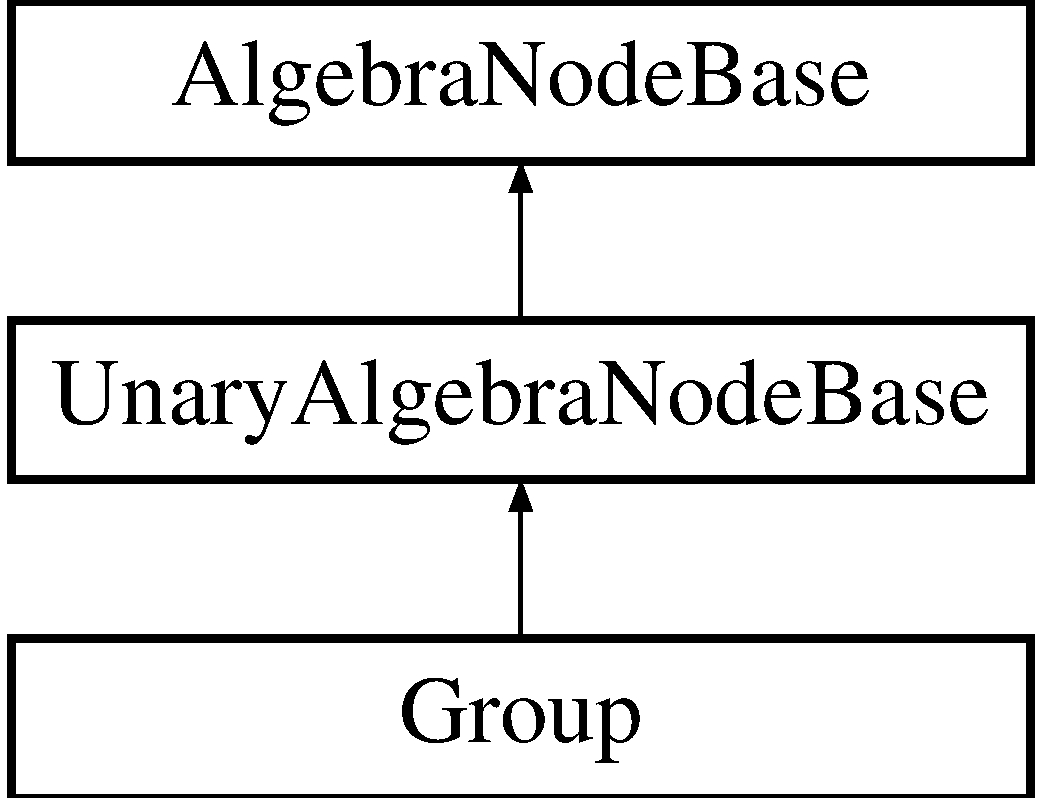
\includegraphics[height=3.000000cm]{class_group}
\end{center}
\end{figure}
\subsection*{Public Member Functions}
\begin{DoxyCompactItemize}
\item 
\hyperlink{class_group_ae331a9b7095f8c2481e2031d41d88164}{Group} (D\+O\+M\+Element $\ast$element)
\item 
void \hyperlink{class_group_a5286b05dd9be36f3a76d075a43191184}{accept} (\hyperlink{class_algebra_visitor}{Algebra\+Visitor} \&v)
\end{DoxyCompactItemize}
\subsection*{Public Attributes}
\begin{DoxyCompactItemize}
\item 
std\+::vector$<$ \hyperlink{class_group_column}{Group\+Column} $>$ \hyperlink{class_group_a811076e176eaa4e3bb8373b7bd515c7e}{group\+Columns}
\item 
std\+::vector$<$ \hyperlink{class_agregate_function}{Agregate\+Function} $>$ \hyperlink{class_group_afd02ca31d700990cddc2860d562635c2}{agregate\+Functions}
\end{DoxyCompactItemize}


\subsection{Detailed Description}
Represents algebraic operation group. It groups by given columns and also computes agregate functions. 

\subsection{Constructor \& Destructor Documentation}
\hypertarget{class_group_ae331a9b7095f8c2481e2031d41d88164}{\index{Group@{Group}!Group@{Group}}
\index{Group@{Group}!Group@{Group}}
\subsubsection[{Group}]{\setlength{\rightskip}{0pt plus 5cm}Group\+::\+Group (
\begin{DoxyParamCaption}
\item[{D\+O\+M\+Element $\ast$}]{element}
\end{DoxyParamCaption}
)}}\label{class_group_ae331a9b7095f8c2481e2031d41d88164}
Create the instance of \hyperlink{class_group}{Group}. 
\begin{DoxyParams}{Parameters}
{\em element} & representing input node. \\
\hline
\end{DoxyParams}


\subsection{Member Function Documentation}
\hypertarget{class_group_a5286b05dd9be36f3a76d075a43191184}{\index{Group@{Group}!accept@{accept}}
\index{accept@{accept}!Group@{Group}}
\subsubsection[{accept}]{\setlength{\rightskip}{0pt plus 5cm}void Group\+::accept (
\begin{DoxyParamCaption}
\item[{{\bf Algebra\+Visitor} \&}]{v}
\end{DoxyParamCaption}
)\hspace{0.3cm}{\ttfamily [virtual]}}}\label{class_group_a5286b05dd9be36f3a76d075a43191184}
Method for calling visit\mbox{[}node\mbox{]} on given \hyperlink{class_algebra_visitor}{Algebra\+Visitor} 
\begin{DoxyParams}{Parameters}
{\em v} & \hyperlink{class_algebra_visitor}{Algebra\+Visitor}, on which to call function \\
\hline
\end{DoxyParams}


Implements \hyperlink{class_unary_algebra_node_base_a33355111a226cb460c9a13efaf922e32}{Unary\+Algebra\+Node\+Base}.



\subsection{Member Data Documentation}
\hypertarget{class_group_afd02ca31d700990cddc2860d562635c2}{\index{Group@{Group}!agregate\+Functions@{agregate\+Functions}}
\index{agregate\+Functions@{agregate\+Functions}!Group@{Group}}
\subsubsection[{agregate\+Functions}]{\setlength{\rightskip}{0pt plus 5cm}std\+::vector$<${\bf Agregate\+Function}$>$ Group\+::agregate\+Functions}}\label{class_group_afd02ca31d700990cddc2860d562635c2}
Stores agregate function information associated with this group node. \hypertarget{class_group_a811076e176eaa4e3bb8373b7bd515c7e}{\index{Group@{Group}!group\+Columns@{group\+Columns}}
\index{group\+Columns@{group\+Columns}!Group@{Group}}
\subsubsection[{group\+Columns}]{\setlength{\rightskip}{0pt plus 5cm}std\+::vector$<${\bf Group\+Column}$>$ Group\+::group\+Columns}}\label{class_group_a811076e176eaa4e3bb8373b7bd515c7e}
Determines by which columns should current relation by grouped by. 

The documentation for this class was generated from the following files\+:\begin{DoxyCompactItemize}
\item 
C\+:/\+Users/\+Marcel/\+Documents/\+Visual Studio 2012/\+Projects/\+Relational\+Query\+Evaluator/\+Relational\+Query\+Evaluator/Algebra.\+h\item 
C\+:/\+Users/\+Marcel/\+Documents/\+Visual Studio 2012/\+Projects/\+Relational\+Query\+Evaluator/\+Relational\+Query\+Evaluator/Algebra.\+cpp\end{DoxyCompactItemize}

\hypertarget{class_group_column}{\section{Group\+Column Class Reference}
\label{class_group_column}\index{Group\+Column@{Group\+Column}}
}


{\ttfamily \#include $<$Algebra\+Structures.\+h$>$}

\subsection*{Public Member Functions}
\begin{DoxyCompactItemize}
\item 
\hyperlink{class_group_column_a6b48cfe01058e5c5a06e2882d329b5ca}{Group\+Column} (const \hyperlink{class_column_identifier}{Column\+Identifier} \&\hyperlink{class_group_column_a2bcc2e12a33f7a9b47633f2b87ebc68b}{input})
\end{DoxyCompactItemize}
\subsection*{Public Attributes}
\begin{DoxyCompactItemize}
\item 
\hyperlink{class_column_identifier}{Column\+Identifier} \hyperlink{class_group_column_a2bcc2e12a33f7a9b47633f2b87ebc68b}{input}
\item 
\hyperlink{class_column_identifier}{Column\+Identifier} \hyperlink{class_group_column_a512e089dfed68312aeadfcbdd1b80a21}{output}
\end{DoxyCompactItemize}


\subsection{Detailed Description}
Stores information about grouping column. 

\subsection{Constructor \& Destructor Documentation}
\hypertarget{class_group_column_a6b48cfe01058e5c5a06e2882d329b5ca}{\index{Group\+Column@{Group\+Column}!Group\+Column@{Group\+Column}}
\index{Group\+Column@{Group\+Column}!Group\+Column@{Group\+Column}}
\subsubsection[{Group\+Column}]{\setlength{\rightskip}{0pt plus 5cm}Group\+Column\+::\+Group\+Column (
\begin{DoxyParamCaption}
\item[{const {\bf Column\+Identifier} \&}]{input}
\end{DoxyParamCaption}
)}}\label{class_group_column_a6b48cfe01058e5c5a06e2882d329b5ca}
Create the instance of \hyperlink{class_group_column}{Group\+Column} using \hyperlink{class_column_identifier}{Column\+Identifier}. 
\begin{DoxyParams}{Parameters}
{\em input} & -\/ \hyperlink{class_column_identifier}{Column\+Identifier} of the column \\
\hline
\end{DoxyParams}


\subsection{Member Data Documentation}
\hypertarget{class_group_column_a2bcc2e12a33f7a9b47633f2b87ebc68b}{\index{Group\+Column@{Group\+Column}!input@{input}}
\index{input@{input}!Group\+Column@{Group\+Column}}
\subsubsection[{input}]{\setlength{\rightskip}{0pt plus 5cm}{\bf Column\+Identifier} Group\+Column\+::input}}\label{class_group_column_a2bcc2e12a33f7a9b47633f2b87ebc68b}
Identifier of input column. \hypertarget{class_group_column_a512e089dfed68312aeadfcbdd1b80a21}{\index{Group\+Column@{Group\+Column}!output@{output}}
\index{output@{output}!Group\+Column@{Group\+Column}}
\subsubsection[{output}]{\setlength{\rightskip}{0pt plus 5cm}{\bf Column\+Identifier} Group\+Column\+::output}}\label{class_group_column_a512e089dfed68312aeadfcbdd1b80a21}
Identifier of output column. Input and output are same but they have different id. 

The documentation for this class was generated from the following files\+:\begin{DoxyCompactItemize}
\item 
C\+:/\+Users/\+Marcel/\+Documents/\+Visual Studio 2012/\+Projects/\+Relational\+Query\+Evaluator/\+Relational\+Query\+Evaluator/Algebra\+Structures.\+h\item 
C\+:/\+Users/\+Marcel/\+Documents/\+Visual Studio 2012/\+Projects/\+Relational\+Query\+Evaluator/\+Relational\+Query\+Evaluator/Algebra\+Structures.\+cpp\end{DoxyCompactItemize}

\hypertarget{class_grouped_algebra_node}{\section{Grouped\+Algebra\+Node Class Reference}
\label{class_grouped_algebra_node}\index{Grouped\+Algebra\+Node@{Grouped\+Algebra\+Node}}
}


{\ttfamily \#include $<$Algebra.\+h$>$}

Inheritance diagram for Grouped\+Algebra\+Node\+:\begin{figure}[H]
\begin{center}
\leavevmode
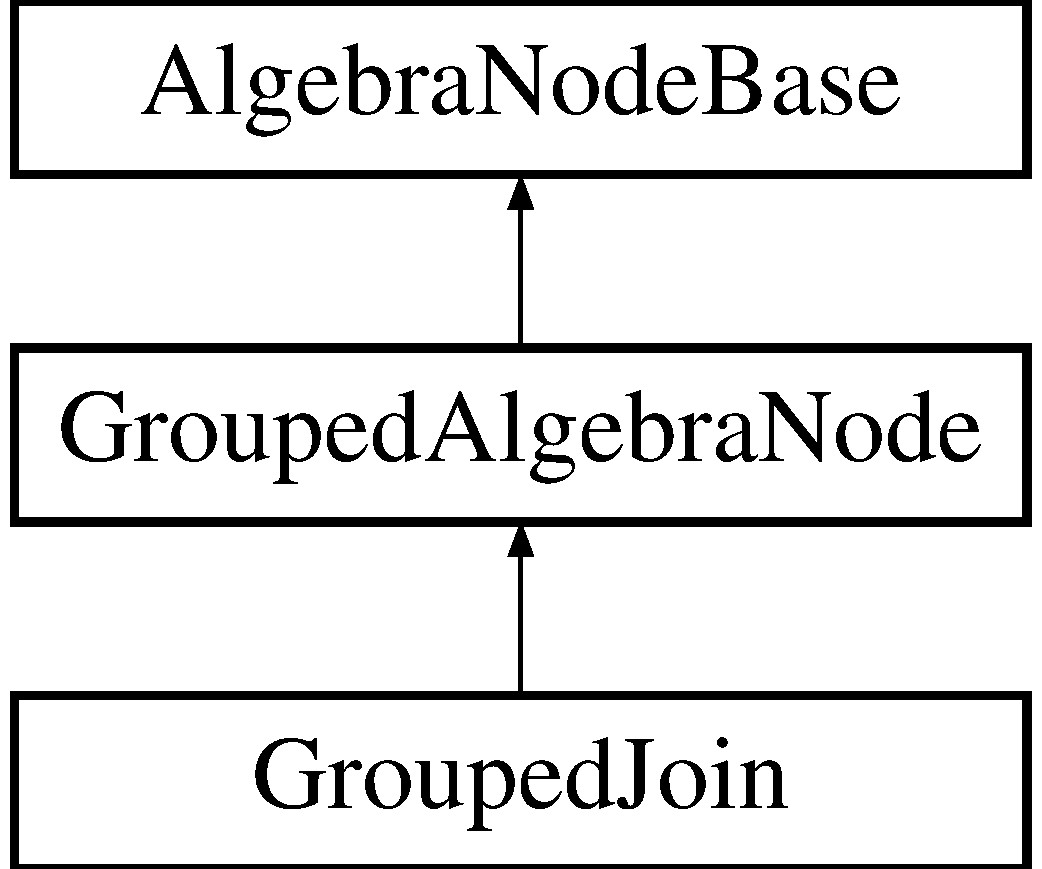
\includegraphics[height=3.000000cm]{class_grouped_algebra_node}
\end{center}
\end{figure}
\subsection*{Public Member Functions}
\begin{DoxyCompactItemize}
\item 
virtual void \hyperlink{class_grouped_algebra_node_a60aae470b5aee869eca9a504fdf79f32}{accept} (\hyperlink{class_algebra_visitor}{Algebra\+Visitor} \&v)=0
\item 
std\+::shared\+\_\+ptr$<$ \hyperlink{class_algebra_node_base}{Algebra\+Node\+Base} $>$ \hyperlink{class_grouped_algebra_node_a463e6303f6332fc9ed2a885e3456b58e}{replace\+Child} (\hyperlink{class_algebra_node_base}{Algebra\+Node\+Base} $\ast$old\+Child, std\+::shared\+\_\+ptr$<$ \hyperlink{class_algebra_node_base}{Algebra\+Node\+Base} $>$ \&new\+Child)
\end{DoxyCompactItemize}
\subsection*{Public Attributes}
\begin{DoxyCompactItemize}
\item 
std\+::vector$<$ std\+::shared\+\_\+ptr\\*
$<$ \hyperlink{class_algebra_node_base}{Algebra\+Node\+Base} $>$ $>$ \hyperlink{class_grouped_algebra_node_acabb532765e4d32cec630651bb5d726f}{children}
\end{DoxyCompactItemize}


\subsection{Detailed Description}
Abstract class for n-\/nary algebraic operation. 

\subsection{Member Function Documentation}
\hypertarget{class_grouped_algebra_node_a60aae470b5aee869eca9a504fdf79f32}{\index{Grouped\+Algebra\+Node@{Grouped\+Algebra\+Node}!accept@{accept}}
\index{accept@{accept}!Grouped\+Algebra\+Node@{Grouped\+Algebra\+Node}}
\subsubsection[{accept}]{\setlength{\rightskip}{0pt plus 5cm}virtual void Grouped\+Algebra\+Node\+::accept (
\begin{DoxyParamCaption}
\item[{{\bf Algebra\+Visitor} \&}]{v}
\end{DoxyParamCaption}
)\hspace{0.3cm}{\ttfamily [pure virtual]}}}\label{class_grouped_algebra_node_a60aae470b5aee869eca9a504fdf79f32}
Method for calling visit\mbox{[}node\mbox{]} on given \hyperlink{class_algebra_visitor}{Algebra\+Visitor} 
\begin{DoxyParams}{Parameters}
{\em v} & \hyperlink{class_algebra_visitor}{Algebra\+Visitor}, on which to call function \\
\hline
\end{DoxyParams}


Implements \hyperlink{class_algebra_node_base_a33bee3ec6fe1eb4228c0471c95c90d66}{Algebra\+Node\+Base}.



Implemented in \hyperlink{class_grouped_join_aa067c1a349478bfdeae77ed3a541375d}{Grouped\+Join}.

\hypertarget{class_grouped_algebra_node_a463e6303f6332fc9ed2a885e3456b58e}{\index{Grouped\+Algebra\+Node@{Grouped\+Algebra\+Node}!replace\+Child@{replace\+Child}}
\index{replace\+Child@{replace\+Child}!Grouped\+Algebra\+Node@{Grouped\+Algebra\+Node}}
\subsubsection[{replace\+Child}]{\setlength{\rightskip}{0pt plus 5cm}shared\+\_\+ptr$<$ {\bf Algebra\+Node\+Base} $>$ Grouped\+Algebra\+Node\+::replace\+Child (
\begin{DoxyParamCaption}
\item[{{\bf Algebra\+Node\+Base} $\ast$}]{old\+Child, }
\item[{std\+::shared\+\_\+ptr$<$ {\bf Algebra\+Node\+Base} $>$ \&}]{new\+Child}
\end{DoxyParamCaption}
)\hspace{0.3cm}{\ttfamily [virtual]}}}\label{class_grouped_algebra_node_a463e6303f6332fc9ed2a885e3456b58e}
Replaces one child of this node with other one 
\begin{DoxyParams}{Parameters}
{\em old\+Child} & node to be replaced \\
\hline
{\em new\+Child} & new node to replace old one \\
\hline
\end{DoxyParams}
\begin{DoxyReturn}{Returns}
replaced child 
\end{DoxyReturn}


Implements \hyperlink{class_algebra_node_base_aa9bdd02b0ddf793bda18bd146ccacb0d}{Algebra\+Node\+Base}.



\subsection{Member Data Documentation}
\hypertarget{class_grouped_algebra_node_acabb532765e4d32cec630651bb5d726f}{\index{Grouped\+Algebra\+Node@{Grouped\+Algebra\+Node}!children@{children}}
\index{children@{children}!Grouped\+Algebra\+Node@{Grouped\+Algebra\+Node}}
\subsubsection[{children}]{\setlength{\rightskip}{0pt plus 5cm}std\+::vector$<$std\+::shared\+\_\+ptr$<${\bf Algebra\+Node\+Base}$>$ $>$ Grouped\+Algebra\+Node\+::children}}\label{class_grouped_algebra_node_acabb532765e4d32cec630651bb5d726f}
Stores list of this node children. 

The documentation for this class was generated from the following files\+:\begin{DoxyCompactItemize}
\item 
C\+:/\+Users/\+Marcel/\+Documents/\+Visual Studio 2012/\+Projects/\+Relational\+Query\+Evaluator/\+Relational\+Query\+Evaluator/Algebra.\+h\item 
C\+:/\+Users/\+Marcel/\+Documents/\+Visual Studio 2012/\+Projects/\+Relational\+Query\+Evaluator/\+Relational\+Query\+Evaluator/Algebra.\+cpp\end{DoxyCompactItemize}

\hypertarget{class_grouped_expression}{\section{Grouped\+Expression Class Reference}
\label{class_grouped_expression}\index{Grouped\+Expression@{Grouped\+Expression}}
}
Inheritance diagram for Grouped\+Expression\+:\begin{figure}[H]
\begin{center}
\leavevmode
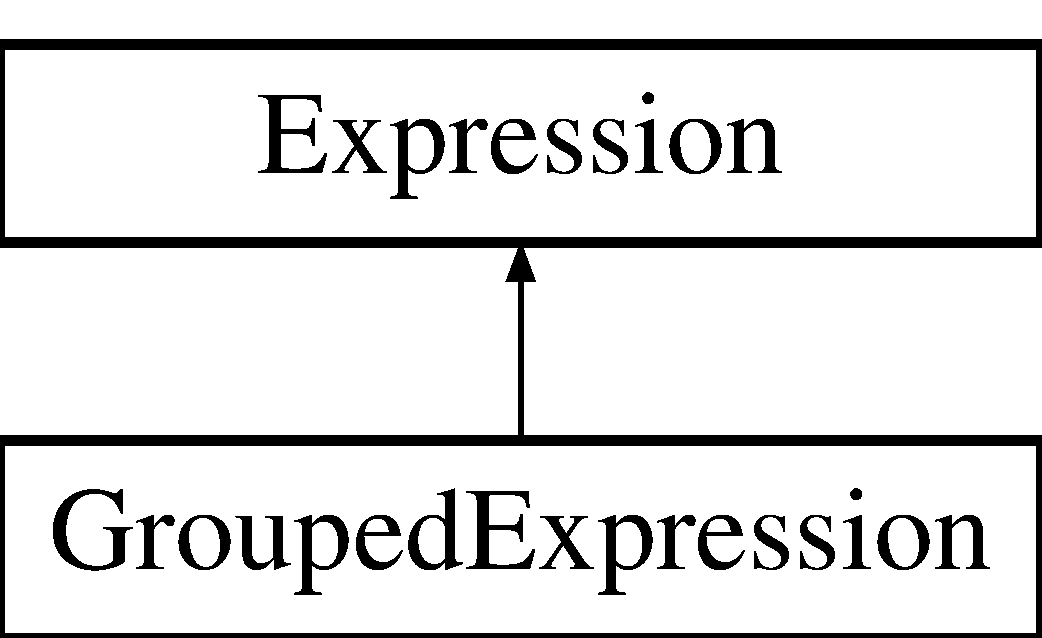
\includegraphics[height=2.000000cm]{class_grouped_expression}
\end{center}
\end{figure}
\subsection*{Public Member Functions}
\begin{DoxyCompactItemize}
\item 
\hypertarget{class_grouped_expression_a986d27a72d99ad866ad0d24241795a80}{{\bfseries Grouped\+Expression} (Grouped\+Operator operation, const std\+::vector$<$ std\+::shared\+\_\+ptr$<$ \hyperlink{class_expression}{Expression} $>$$>$ \&children)}\label{class_grouped_expression_a986d27a72d99ad866ad0d24241795a80}

\item 
\hypertarget{class_grouped_expression_a67963e289263b9c2cbf03edad83401b7}{void {\bfseries accept} (\hyperlink{class_expression_visitor_base}{Expression\+Visitor\+Base} \&v)}\label{class_grouped_expression_a67963e289263b9c2cbf03edad83401b7}

\item 
\hypertarget{class_grouped_expression_af1cb9044417df12361b6335962b3bc6c}{void {\bfseries replace\+Child} (\hyperlink{class_expression}{Expression} $\ast$old\+Child, std\+::shared\+\_\+ptr$<$ \hyperlink{class_expression}{Expression} $>$ new\+Child)}\label{class_grouped_expression_af1cb9044417df12361b6335962b3bc6c}

\end{DoxyCompactItemize}
\subsection*{Public Attributes}
\begin{DoxyCompactItemize}
\item 
\hypertarget{class_grouped_expression_a018f4f129a3b9b0be45c8ed10ff21813}{Grouped\+Operator {\bfseries operation}}\label{class_grouped_expression_a018f4f129a3b9b0be45c8ed10ff21813}

\item 
\hypertarget{class_grouped_expression_aabace43c5af51a0e913ff9033b71295c}{std\+::vector$<$ std\+::shared\+\_\+ptr\\*
$<$ \hyperlink{class_expression}{Expression} $>$ $>$ {\bfseries children}}\label{class_grouped_expression_aabace43c5af51a0e913ff9033b71295c}

\end{DoxyCompactItemize}
\subsection*{Additional Inherited Members}


The documentation for this class was generated from the following files\+:\begin{DoxyCompactItemize}
\item 
C\+:/\+Users/\+Marcel/\+Documents/\+Visual Studio 2012/\+Projects/\+Relational\+Query\+Evaluator/\+Relational\+Query\+Evaluator/Expressions.\+h\item 
C\+:/\+Users/\+Marcel/\+Documents/\+Visual Studio 2012/\+Projects/\+Relational\+Query\+Evaluator/\+Relational\+Query\+Evaluator/Expressions.\+cpp\end{DoxyCompactItemize}

\hypertarget{class_grouped_join}{\section{Grouped\+Join Class Reference}
\label{class_grouped_join}\index{Grouped\+Join@{Grouped\+Join}}
}
Inheritance diagram for Grouped\+Join\+:\begin{figure}[H]
\begin{center}
\leavevmode
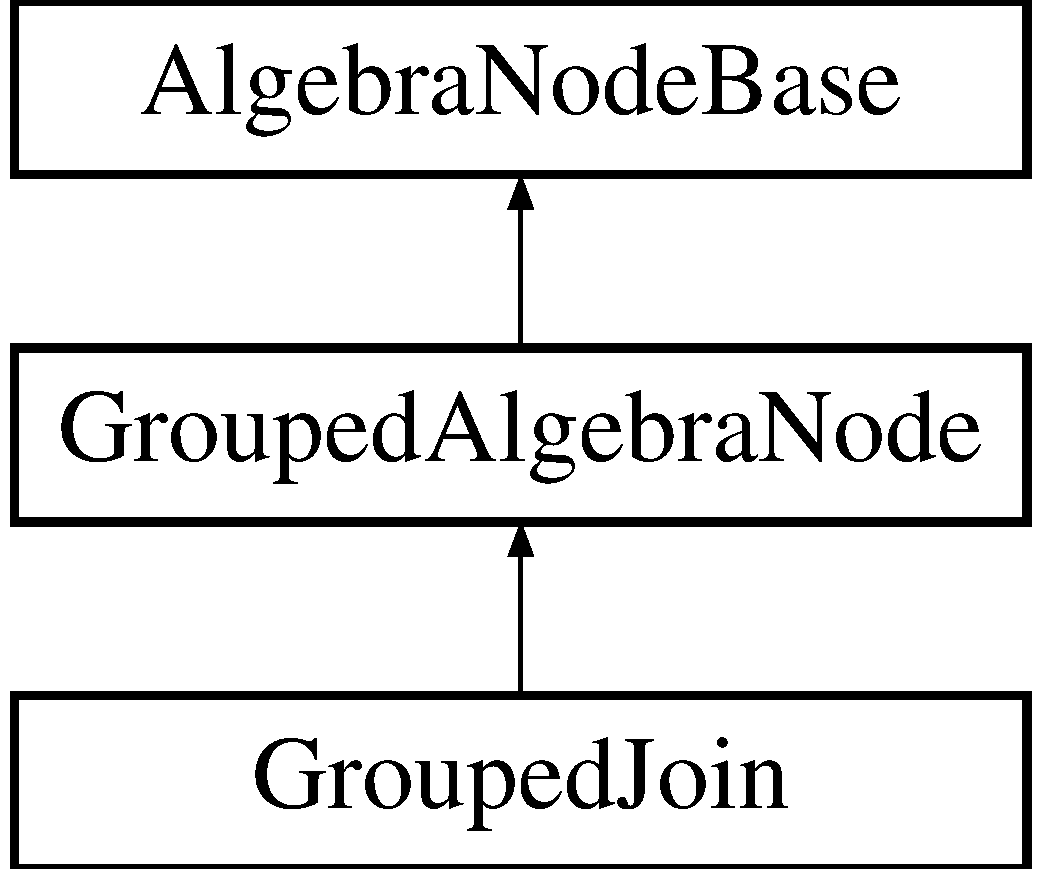
\includegraphics[height=3.000000cm]{class_grouped_join}
\end{center}
\end{figure}
\subsection*{Public Member Functions}
\begin{DoxyCompactItemize}
\item 
\hypertarget{class_grouped_join_aa067c1a349478bfdeae77ed3a541375d}{void {\bfseries accept} (\hyperlink{class_algebra_visitor}{Algebra\+Visitor} \&v)}\label{class_grouped_join_aa067c1a349478bfdeae77ed3a541375d}

\end{DoxyCompactItemize}
\subsection*{Public Attributes}
\begin{DoxyCompactItemize}
\item 
\hypertarget{class_grouped_join_a517b47e21d6852335b50537c474c9c62}{std\+::shared\+\_\+ptr$<$ \hyperlink{class_expression}{Expression} $>$ {\bfseries condition}}\label{class_grouped_join_a517b47e21d6852335b50537c474c9c62}

\item 
\hypertarget{class_grouped_join_ae1cd2d5ce317a02f65249e45451e3391}{std\+::shared\+\_\+ptr$<$ \hyperlink{class_expression}{Expression} $>$ {\bfseries non\+Joincondition}}\label{class_grouped_join_ae1cd2d5ce317a02f65249e45451e3391}

\item 
\hypertarget{class_grouped_join_ab4e436f7abb9990000a7f2ef0596960e}{std\+::vector$<$ \hyperlink{class_join_column_info}{Join\+Column\+Info} $>$ {\bfseries output\+Join\+Columns}}\label{class_grouped_join_ab4e436f7abb9990000a7f2ef0596960e}

\end{DoxyCompactItemize}


The documentation for this class was generated from the following files\+:\begin{DoxyCompactItemize}
\item 
C\+:/\+Users/\+Marcel/\+Documents/\+Visual Studio 2012/\+Projects/\+Relational\+Query\+Evaluator/\+Relational\+Query\+Evaluator/Algebra.\+h\item 
C\+:/\+Users/\+Marcel/\+Documents/\+Visual Studio 2012/\+Projects/\+Relational\+Query\+Evaluator/\+Relational\+Query\+Evaluator/Algebra.\+cpp\end{DoxyCompactItemize}

\hypertarget{class_grouping_expression_visitor}{\section{Grouping\+Expression\+Visitor Class Reference}
\label{class_grouping_expression_visitor}\index{Grouping\+Expression\+Visitor@{Grouping\+Expression\+Visitor}}
}
Inheritance diagram for Grouping\+Expression\+Visitor\+:\begin{figure}[H]
\begin{center}
\leavevmode
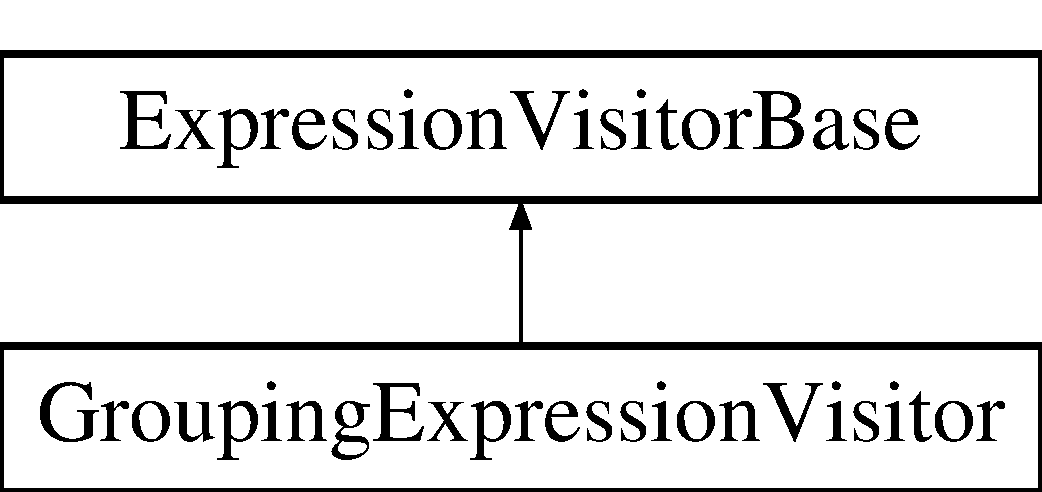
\includegraphics[height=2.000000cm]{class_grouping_expression_visitor}
\end{center}
\end{figure}
\subsection*{Public Member Functions}
\begin{DoxyCompactItemize}
\item 
\hypertarget{class_grouping_expression_visitor_a237e5aaa25294095a1b3c14c4ef64794}{{\bfseries Grouping\+Expression\+Visitor} (std\+::shared\+\_\+ptr$<$ \hyperlink{class_expression}{Expression} $>$ $\ast$x)}\label{class_grouping_expression_visitor_a237e5aaa25294095a1b3c14c4ef64794}

\item 
\hypertarget{class_grouping_expression_visitor_aba30832e7f966be15e50b17d68badbb1}{void {\bfseries visit\+Binary\+Expression} (\hyperlink{class_binary_expression}{Binary\+Expression} $\ast$expression)}\label{class_grouping_expression_visitor_aba30832e7f966be15e50b17d68badbb1}

\end{DoxyCompactItemize}
\subsection*{Public Attributes}
\begin{DoxyCompactItemize}
\item 
\hypertarget{class_grouping_expression_visitor_a493ef343ca18357dca158d83085b5ab4}{std\+::shared\+\_\+ptr$<$ \hyperlink{class_expression}{Expression} $>$ $\ast$ {\bfseries root}}\label{class_grouping_expression_visitor_a493ef343ca18357dca158d83085b5ab4}

\end{DoxyCompactItemize}


The documentation for this class was generated from the following files\+:\begin{DoxyCompactItemize}
\item 
C\+:/\+Users/\+Marcel/\+Documents/\+Visual Studio 2012/\+Projects/\+Relational\+Query\+Evaluator/\+Relational\+Query\+Evaluator/Expression\+Visitors.\+h\item 
C\+:/\+Users/\+Marcel/\+Documents/\+Visual Studio 2012/\+Projects/\+Relational\+Query\+Evaluator/\+Relational\+Query\+Evaluator/Expression\+Visitors.\+cpp\end{DoxyCompactItemize}

\hypertarget{class_grouping_visitor}{\section{Grouping\+Visitor Class Reference}
\label{class_grouping_visitor}\index{Grouping\+Visitor@{Grouping\+Visitor}}
}


{\ttfamily \#include $<$Algebra\+Visitors.\+h$>$}

Inheritance diagram for Grouping\+Visitor\+:\begin{figure}[H]
\begin{center}
\leavevmode
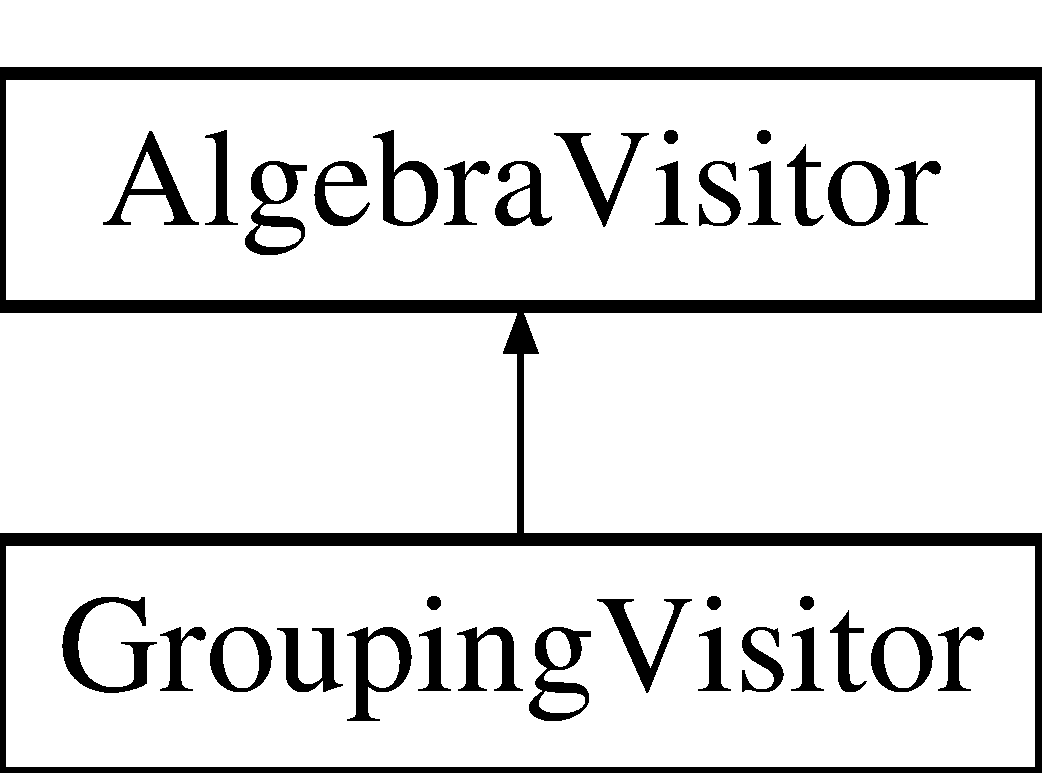
\includegraphics[height=2.000000cm]{class_grouping_visitor}
\end{center}
\end{figure}
\subsection*{Public Member Functions}
\begin{DoxyCompactItemize}
\item 
\hyperlink{class_grouping_visitor_adc7a72ec400998ac4dcaacf5c85fb86c}{Grouping\+Visitor} ()
\item 
void \hyperlink{class_grouping_visitor_a2c1557a18e53aaa43665318001df3726}{visit\+Column\+Operations} (\hyperlink{class_column_operations}{Column\+Operations} $\ast$node)
\item 
void \hyperlink{class_grouping_visitor_a4e3563b131b9d26942a6d4693f5c194a}{visit\+Selection} (\hyperlink{class_selection}{Selection} $\ast$node)
\item 
void \hyperlink{class_grouping_visitor_aaa2345624497de18ab3a608e909573aa}{visit\+Join} (\hyperlink{class_join}{Join} $\ast$node)
\item 
void \hyperlink{class_grouping_visitor_a1ddb0cf950feb1df7c2518b543e0d0ad}{visit\+Anti\+Join} (\hyperlink{class_anti_join}{Anti\+Join} $\ast$node)
\item 
void \hyperlink{class_grouping_visitor_a7c6760e32033d79e45159d7907aa8886}{resolve\+Joins} (\hyperlink{class_join}{Join} $\ast$node, \hyperlink{class_grouped_join}{Grouped\+Join} $\ast$grouped\+Operator)
\end{DoxyCompactItemize}
\subsection*{Additional Inherited Members}


\subsection{Detailed Description}
This algebra visitor groupes neighbour join into one groupped join. It also calls \hyperlink{class_grouping_expression_visitor}{Grouping\+Expression\+Visitor} on every condition. 

\subsection{Constructor \& Destructor Documentation}
\hypertarget{class_grouping_visitor_adc7a72ec400998ac4dcaacf5c85fb86c}{\index{Grouping\+Visitor@{Grouping\+Visitor}!Grouping\+Visitor@{Grouping\+Visitor}}
\index{Grouping\+Visitor@{Grouping\+Visitor}!Grouping\+Visitor@{Grouping\+Visitor}}
\subsubsection[{Grouping\+Visitor}]{\setlength{\rightskip}{0pt plus 5cm}Grouping\+Visitor\+::\+Grouping\+Visitor (
\begin{DoxyParamCaption}
{}
\end{DoxyParamCaption}
)}}\label{class_grouping_visitor_adc7a72ec400998ac4dcaacf5c85fb86c}
Creates new instance of \hyperlink{class_grouping_visitor}{Grouping\+Visitor}. 

\subsection{Member Function Documentation}
\hypertarget{class_grouping_visitor_a7c6760e32033d79e45159d7907aa8886}{\index{Grouping\+Visitor@{Grouping\+Visitor}!resolve\+Joins@{resolve\+Joins}}
\index{resolve\+Joins@{resolve\+Joins}!Grouping\+Visitor@{Grouping\+Visitor}}
\subsubsection[{resolve\+Joins}]{\setlength{\rightskip}{0pt plus 5cm}void Grouping\+Visitor\+::resolve\+Joins (
\begin{DoxyParamCaption}
\item[{{\bf Join} $\ast$}]{node, }
\item[{{\bf Grouped\+Join} $\ast$}]{grouped\+Operator}
\end{DoxyParamCaption}
)}}\label{class_grouping_visitor_a7c6760e32033d79e45159d7907aa8886}
Hepler method, which merges join node to \hyperlink{class_grouped_join}{Grouped\+Join} and update all nedded parameters like condition and outputcolumns. 
\begin{DoxyParams}{Parameters}
{\em node} & -\/ node to merge \\
\hline
{\em grouped\+Operator} & -\/ node to be merge to \\
\hline
\end{DoxyParams}
\hypertarget{class_grouping_visitor_a1ddb0cf950feb1df7c2518b543e0d0ad}{\index{Grouping\+Visitor@{Grouping\+Visitor}!visit\+Anti\+Join@{visit\+Anti\+Join}}
\index{visit\+Anti\+Join@{visit\+Anti\+Join}!Grouping\+Visitor@{Grouping\+Visitor}}
\subsubsection[{visit\+Anti\+Join}]{\setlength{\rightskip}{0pt plus 5cm}void Grouping\+Visitor\+::visit\+Anti\+Join (
\begin{DoxyParamCaption}
\item[{{\bf Anti\+Join} $\ast$}]{node}
\end{DoxyParamCaption}
)\hspace{0.3cm}{\ttfamily [virtual]}}}\label{class_grouping_visitor_a1ddb0cf950feb1df7c2518b543e0d0ad}
Visits \hyperlink{class_anti_join}{Anti\+Join} element. 
\begin{DoxyParams}{Parameters}
{\em node} & visited \hyperlink{class_anti_join}{Anti\+Join}. \\
\hline
\end{DoxyParams}


Reimplemented from \hyperlink{class_algebra_visitor_add62415db5f188e572cef1c36faa842e}{Algebra\+Visitor}.

\hypertarget{class_grouping_visitor_a2c1557a18e53aaa43665318001df3726}{\index{Grouping\+Visitor@{Grouping\+Visitor}!visit\+Column\+Operations@{visit\+Column\+Operations}}
\index{visit\+Column\+Operations@{visit\+Column\+Operations}!Grouping\+Visitor@{Grouping\+Visitor}}
\subsubsection[{visit\+Column\+Operations}]{\setlength{\rightskip}{0pt plus 5cm}void Grouping\+Visitor\+::visit\+Column\+Operations (
\begin{DoxyParamCaption}
\item[{{\bf Column\+Operations} $\ast$}]{node}
\end{DoxyParamCaption}
)\hspace{0.3cm}{\ttfamily [virtual]}}}\label{class_grouping_visitor_a2c1557a18e53aaa43665318001df3726}
Visits \hyperlink{class_column_operations}{Column\+Operations} element. 
\begin{DoxyParams}{Parameters}
{\em node} & visited \hyperlink{class_column_operations}{Column\+Operations}. \\
\hline
\end{DoxyParams}


Reimplemented from \hyperlink{class_algebra_visitor_a1109510d982a8e5b90fc56d443109ef9}{Algebra\+Visitor}.

\hypertarget{class_grouping_visitor_aaa2345624497de18ab3a608e909573aa}{\index{Grouping\+Visitor@{Grouping\+Visitor}!visit\+Join@{visit\+Join}}
\index{visit\+Join@{visit\+Join}!Grouping\+Visitor@{Grouping\+Visitor}}
\subsubsection[{visit\+Join}]{\setlength{\rightskip}{0pt plus 5cm}void Grouping\+Visitor\+::visit\+Join (
\begin{DoxyParamCaption}
\item[{{\bf Join} $\ast$}]{node}
\end{DoxyParamCaption}
)\hspace{0.3cm}{\ttfamily [virtual]}}}\label{class_grouping_visitor_aaa2345624497de18ab3a608e909573aa}
Visits \hyperlink{class_join}{Join} element. 
\begin{DoxyParams}{Parameters}
{\em node} & visited \hyperlink{class_join}{Join}. \\
\hline
\end{DoxyParams}


Reimplemented from \hyperlink{class_algebra_visitor_a841875539a07c979b912ef44455b873c}{Algebra\+Visitor}.

\hypertarget{class_grouping_visitor_a4e3563b131b9d26942a6d4693f5c194a}{\index{Grouping\+Visitor@{Grouping\+Visitor}!visit\+Selection@{visit\+Selection}}
\index{visit\+Selection@{visit\+Selection}!Grouping\+Visitor@{Grouping\+Visitor}}
\subsubsection[{visit\+Selection}]{\setlength{\rightskip}{0pt plus 5cm}void Grouping\+Visitor\+::visit\+Selection (
\begin{DoxyParamCaption}
\item[{{\bf Selection} $\ast$}]{node}
\end{DoxyParamCaption}
)\hspace{0.3cm}{\ttfamily [virtual]}}}\label{class_grouping_visitor_a4e3563b131b9d26942a6d4693f5c194a}
Visits \hyperlink{class_selection}{Selection} element. 
\begin{DoxyParams}{Parameters}
{\em node} & visited \hyperlink{class_selection}{Selection}. \\
\hline
\end{DoxyParams}


Reimplemented from \hyperlink{class_algebra_visitor_a7d9b0618ac2fdd036abdab27cbb83d40}{Algebra\+Visitor}.



The documentation for this class was generated from the following files\+:\begin{DoxyCompactItemize}
\item 
C\+:/\+Users/\+Marcel/\+Documents/\+Visual Studio 2012/\+Projects/\+Relational\+Query\+Evaluator/\+Relational\+Query\+Evaluator/Algebra\+Visitors.\+h\item 
C\+:/\+Users/\+Marcel/\+Documents/\+Visual Studio 2012/\+Projects/\+Relational\+Query\+Evaluator/\+Relational\+Query\+Evaluator/Algebra\+Visitors.\+cpp\end{DoxyCompactItemize}

\hypertarget{class_hash_anti_join}{\section{Hash\+Anti\+Join Class Reference}
\label{class_hash_anti_join}\index{Hash\+Anti\+Join@{Hash\+Anti\+Join}}
}
Inheritance diagram for Hash\+Anti\+Join\+:\begin{figure}[H]
\begin{center}
\leavevmode
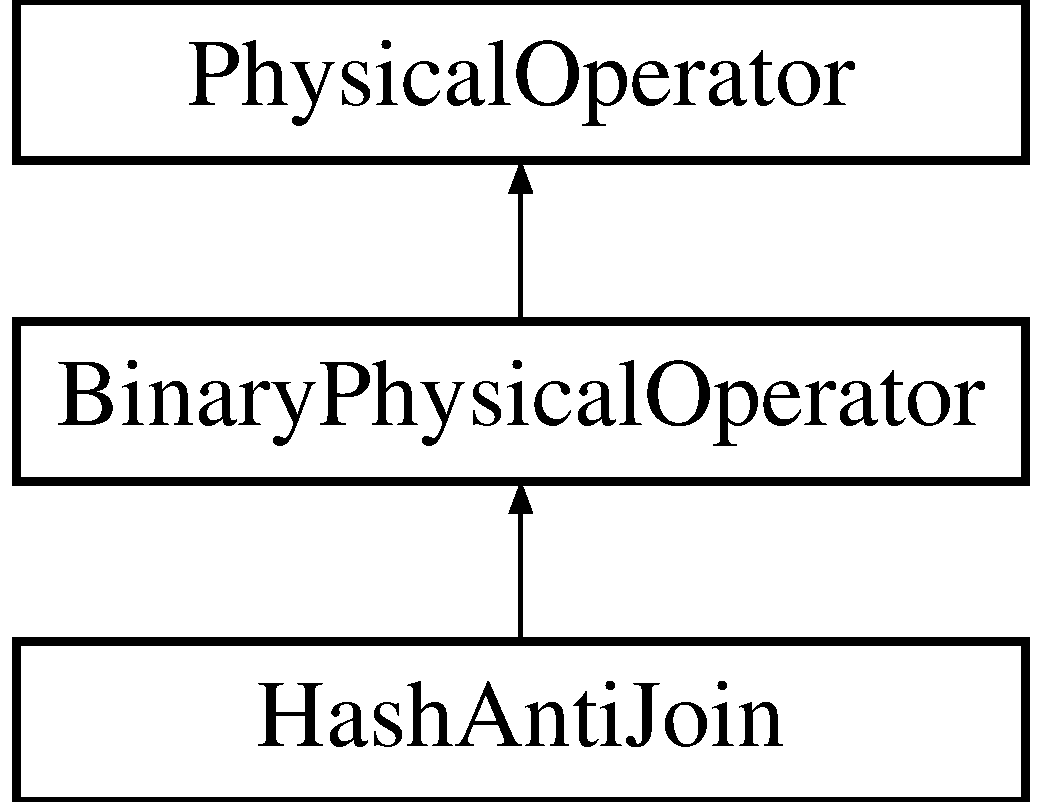
\includegraphics[height=3.000000cm]{class_hash_anti_join}
\end{center}
\end{figure}
\subsection*{Public Member Functions}
\begin{DoxyCompactItemize}
\item 
\hypertarget{class_hash_anti_join_adf6f72c234cc4a3e09e1eab671255912}{{\bfseries Hash\+Anti\+Join} (const std\+::shared\+\_\+ptr$<$ \hyperlink{class_expression}{Expression} $>$ \&condition, const std\+::vector$<$ \hyperlink{class_column_identifier}{Column\+Identifier} $>$ \&left, const std\+::vector$<$ \hyperlink{class_column_identifier}{Column\+Identifier} $>$ \&right)}\label{class_hash_anti_join_adf6f72c234cc4a3e09e1eab671255912}

\item 
\hypertarget{class_hash_anti_join_a8a629e5592d9a42ce155dd83f7f551d0}{void {\bfseries accept} (\hyperlink{class_physical_operator_visitor}{Physical\+Operator\+Visitor} \&v)}\label{class_hash_anti_join_a8a629e5592d9a42ce155dd83f7f551d0}

\end{DoxyCompactItemize}
\subsection*{Public Attributes}
\begin{DoxyCompactItemize}
\item 
\hypertarget{class_hash_anti_join_a94f542040c9ee014a520ddf0b9267ff2}{std\+::shared\+\_\+ptr$<$ \hyperlink{class_expression}{Expression} $>$ {\bfseries condition}}\label{class_hash_anti_join_a94f542040c9ee014a520ddf0b9267ff2}

\item 
\hypertarget{class_hash_anti_join_a87f91c29c85463c75c10539e0239d63a}{std\+::vector$<$ \hyperlink{class_column_identifier}{Column\+Identifier} $>$ {\bfseries left}}\label{class_hash_anti_join_a87f91c29c85463c75c10539e0239d63a}

\item 
\hypertarget{class_hash_anti_join_a3f41da2aa9eff3bad59eef69b0f4486b}{std\+::vector$<$ \hyperlink{class_column_identifier}{Column\+Identifier} $>$ {\bfseries right}}\label{class_hash_anti_join_a3f41da2aa9eff3bad59eef69b0f4486b}

\end{DoxyCompactItemize}


The documentation for this class was generated from the following files\+:\begin{DoxyCompactItemize}
\item 
C\+:/\+Users/\+Marcel/\+Documents/\+Visual Studio 2012/\+Projects/\+Relational\+Query\+Evaluator/\+Relational\+Query\+Evaluator/Physical\+Operator.\+h\item 
C\+:/\+Users/\+Marcel/\+Documents/\+Visual Studio 2012/\+Projects/\+Relational\+Query\+Evaluator/\+Relational\+Query\+Evaluator/Physical\+Operator.\+cpp\end{DoxyCompactItemize}

\hypertarget{class_hash_group}{\section{Hash\+Group Class Reference}
\label{class_hash_group}\index{Hash\+Group@{Hash\+Group}}
}
Inheritance diagram for Hash\+Group\+:\begin{figure}[H]
\begin{center}
\leavevmode
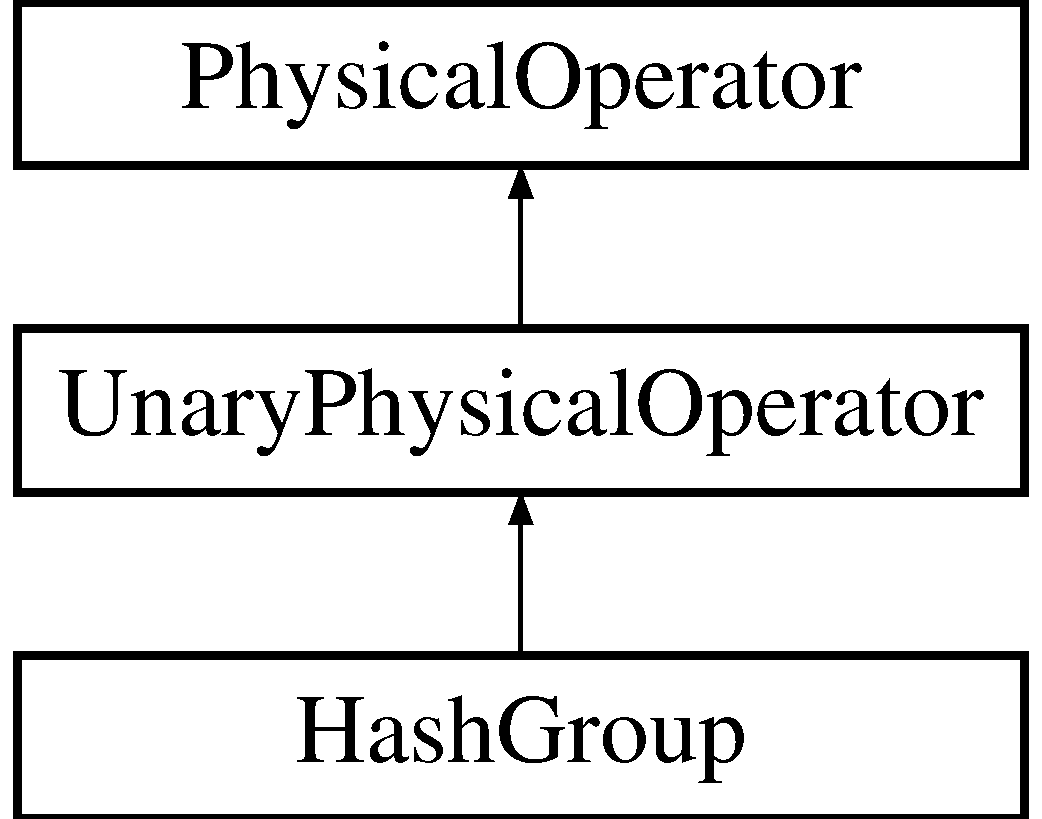
\includegraphics[height=3.000000cm]{class_hash_group}
\end{center}
\end{figure}
\subsection*{Public Member Functions}
\begin{DoxyCompactItemize}
\item 
\hypertarget{class_hash_group_af175f06e72f0fd7476e652ec5ffcbeb7}{{\bfseries Hash\+Group} (const std\+::vector$<$ \hyperlink{class_group_column}{Group\+Column} $>$ \&group\+Columns, const std\+::vector$<$ \hyperlink{class_agregate_function}{Agregate\+Function} $>$ \&agregate\+Functions)}\label{class_hash_group_af175f06e72f0fd7476e652ec5ffcbeb7}

\item 
\hypertarget{class_hash_group_a300c7ad6b7a4e39c9a7dc5a57389b85f}{void {\bfseries accept} (\hyperlink{class_physical_operator_visitor}{Physical\+Operator\+Visitor} \&v)}\label{class_hash_group_a300c7ad6b7a4e39c9a7dc5a57389b85f}

\end{DoxyCompactItemize}
\subsection*{Public Attributes}
\begin{DoxyCompactItemize}
\item 
\hypertarget{class_hash_group_a61af9515cad55af148210493431c5df6}{std\+::vector$<$ \hyperlink{class_group_column}{Group\+Column} $>$ {\bfseries group\+Columns}}\label{class_hash_group_a61af9515cad55af148210493431c5df6}

\item 
\hypertarget{class_hash_group_a8a813f6713413f2bd401bfa77be774de}{std\+::vector$<$ \hyperlink{class_agregate_function}{Agregate\+Function} $>$ {\bfseries agregate\+Functions}}\label{class_hash_group_a8a813f6713413f2bd401bfa77be774de}

\end{DoxyCompactItemize}


The documentation for this class was generated from the following files\+:\begin{DoxyCompactItemize}
\item 
C\+:/\+Users/\+Marcel/\+Documents/\+Visual Studio 2012/\+Projects/\+Relational\+Query\+Evaluator/\+Relational\+Query\+Evaluator/Physical\+Operator.\+h\item 
C\+:/\+Users/\+Marcel/\+Documents/\+Visual Studio 2012/\+Projects/\+Relational\+Query\+Evaluator/\+Relational\+Query\+Evaluator/Physical\+Operator.\+cpp\end{DoxyCompactItemize}

\hypertarget{class_hash_join}{\section{Hash\+Join Class Reference}
\label{class_hash_join}\index{Hash\+Join@{Hash\+Join}}
}


{\ttfamily \#include $<$Physical\+Operator.\+h$>$}

Inheritance diagram for Hash\+Join\+:\begin{figure}[H]
\begin{center}
\leavevmode
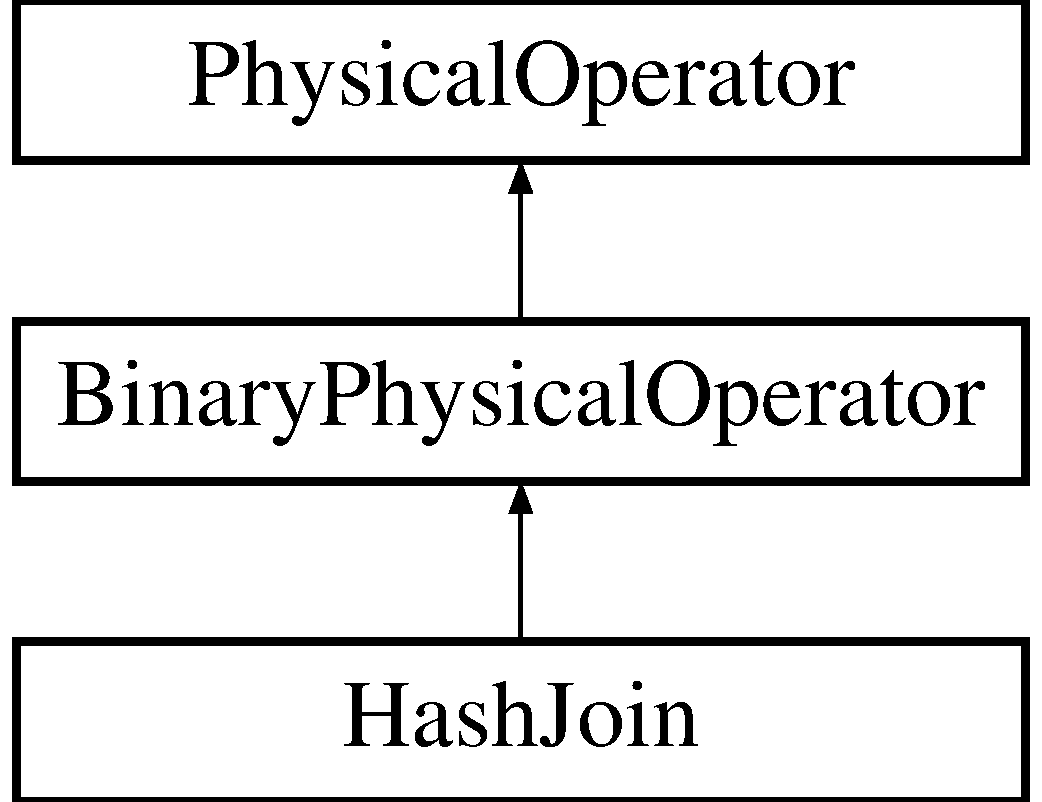
\includegraphics[height=3.000000cm]{class_hash_join}
\end{center}
\end{figure}
\subsection*{Public Member Functions}
\begin{DoxyCompactItemize}
\item 
\hyperlink{class_hash_join_aade828aa470db22861011b21f1335111}{Hash\+Join} (const std\+::shared\+\_\+ptr$<$ \hyperlink{class_expression}{Expression} $>$ \&\hyperlink{class_hash_join_ac2524a0455d2379287a55d8cb148c40d}{condition}, const std\+::vector$<$ \hyperlink{class_column_identifier}{Column\+Identifier} $>$ \&\hyperlink{class_hash_join_a8ce73a163fdc30d10144277b51689541}{left\+Part\+Of\+Condition}, const std\+::vector$<$ \hyperlink{class_column_identifier}{Column\+Identifier} $>$ \&\hyperlink{class_hash_join_ad4f1b144fc9a52d5218b1d2368c295b7}{right\+Part\+Of\+Condition})
\item 
void \hyperlink{class_hash_join_a11dc03e38397ff42352772a3c759e145}{accept} (\hyperlink{class_physical_operator_visitor}{Physical\+Operator\+Visitor} \&v)
\end{DoxyCompactItemize}
\subsection*{Public Attributes}
\begin{DoxyCompactItemize}
\item 
std\+::shared\+\_\+ptr$<$ \hyperlink{class_expression}{Expression} $>$ \hyperlink{class_hash_join_ac2524a0455d2379287a55d8cb148c40d}{condition}
\item 
std\+::vector$<$ \hyperlink{class_column_identifier}{Column\+Identifier} $>$ \hyperlink{class_hash_join_a8ce73a163fdc30d10144277b51689541}{left\+Part\+Of\+Condition}
\item 
std\+::vector$<$ \hyperlink{class_column_identifier}{Column\+Identifier} $>$ \hyperlink{class_hash_join_ad4f1b144fc9a52d5218b1d2368c295b7}{right\+Part\+Of\+Condition}
\end{DoxyCompactItemize}


\subsection{Detailed Description}
Represents hash join physical operator. Operator computes equijoin using hash table. First input will be stored in hash table. 

\subsection{Constructor \& Destructor Documentation}
\hypertarget{class_hash_join_aade828aa470db22861011b21f1335111}{\index{Hash\+Join@{Hash\+Join}!Hash\+Join@{Hash\+Join}}
\index{Hash\+Join@{Hash\+Join}!Hash\+Join@{Hash\+Join}}
\subsubsection[{Hash\+Join}]{\setlength{\rightskip}{0pt plus 5cm}Hash\+Join\+::\+Hash\+Join (
\begin{DoxyParamCaption}
\item[{const std\+::shared\+\_\+ptr$<$ {\bf Expression} $>$ \&}]{condition, }
\item[{const std\+::vector$<$ {\bf Column\+Identifier} $>$ \&}]{left\+Part\+Of\+Condition, }
\item[{const std\+::vector$<$ {\bf Column\+Identifier} $>$ \&}]{right\+Part\+Of\+Condition}
\end{DoxyParamCaption}
)}}\label{class_hash_join_aade828aa470db22861011b21f1335111}
Creates new instance of \hyperlink{class_hash_join}{Hash\+Join}. 
\begin{DoxyParams}{Parameters}
{\em condition} & -\/ join condition. \\
\hline
{\em left\+Part\+Of\+Condition} & -\/ condition columns from first input \\
\hline
{\em right\+Part\+Of\+Condition} & -\/ condition columns from second input \\
\hline
\end{DoxyParams}


\subsection{Member Function Documentation}
\hypertarget{class_hash_join_a11dc03e38397ff42352772a3c759e145}{\index{Hash\+Join@{Hash\+Join}!accept@{accept}}
\index{accept@{accept}!Hash\+Join@{Hash\+Join}}
\subsubsection[{accept}]{\setlength{\rightskip}{0pt plus 5cm}void Hash\+Join\+::accept (
\begin{DoxyParamCaption}
\item[{{\bf Physical\+Operator\+Visitor} \&}]{v}
\end{DoxyParamCaption}
)\hspace{0.3cm}{\ttfamily [virtual]}}}\label{class_hash_join_a11dc03e38397ff42352772a3c759e145}
Method for calling visit\mbox{[}node\mbox{]} on given \hyperlink{class_physical_operator_visitor}{Physical\+Operator\+Visitor}. 
\begin{DoxyParams}{Parameters}
{\em v} & \hyperlink{class_physical_operator_visitor}{Physical\+Operator\+Visitor}, on which to call function. \\
\hline
\end{DoxyParams}


Implements \hyperlink{class_binary_physical_operator_a29ec622920006cb5428bf2c259918347}{Binary\+Physical\+Operator}.



\subsection{Member Data Documentation}
\hypertarget{class_hash_join_ac2524a0455d2379287a55d8cb148c40d}{\index{Hash\+Join@{Hash\+Join}!condition@{condition}}
\index{condition@{condition}!Hash\+Join@{Hash\+Join}}
\subsubsection[{condition}]{\setlength{\rightskip}{0pt plus 5cm}std\+::shared\+\_\+ptr$<${\bf Expression}$>$ Hash\+Join\+::condition}}\label{class_hash_join_ac2524a0455d2379287a55d8cb148c40d}
\hyperlink{class_join}{Join} condition. \hypertarget{class_hash_join_a8ce73a163fdc30d10144277b51689541}{\index{Hash\+Join@{Hash\+Join}!left\+Part\+Of\+Condition@{left\+Part\+Of\+Condition}}
\index{left\+Part\+Of\+Condition@{left\+Part\+Of\+Condition}!Hash\+Join@{Hash\+Join}}
\subsubsection[{left\+Part\+Of\+Condition}]{\setlength{\rightskip}{0pt plus 5cm}std\+::vector$<${\bf Column\+Identifier}$>$ Hash\+Join\+::left\+Part\+Of\+Condition}}\label{class_hash_join_a8ce73a163fdc30d10144277b51689541}
Stores columns from left input, which belongs to condition. \hypertarget{class_hash_join_ad4f1b144fc9a52d5218b1d2368c295b7}{\index{Hash\+Join@{Hash\+Join}!right\+Part\+Of\+Condition@{right\+Part\+Of\+Condition}}
\index{right\+Part\+Of\+Condition@{right\+Part\+Of\+Condition}!Hash\+Join@{Hash\+Join}}
\subsubsection[{right\+Part\+Of\+Condition}]{\setlength{\rightskip}{0pt plus 5cm}std\+::vector$<${\bf Column\+Identifier}$>$ Hash\+Join\+::right\+Part\+Of\+Condition}}\label{class_hash_join_ad4f1b144fc9a52d5218b1d2368c295b7}
Stores columns from right input, which belongs to condition. 

The documentation for this class was generated from the following files\+:\begin{DoxyCompactItemize}
\item 
C\+:/\+Users/\+Marcel/\+Documents/\+Visual Studio 2012/\+Projects/\+Relational\+Query\+Evaluator/\+Relational\+Query\+Evaluator/Physical\+Operator.\+h\item 
C\+:/\+Users/\+Marcel/\+Documents/\+Visual Studio 2012/\+Projects/\+Relational\+Query\+Evaluator/\+Relational\+Query\+Evaluator/Physical\+Operator.\+cpp\end{DoxyCompactItemize}

\hypertarget{class_index}{\section{Index Class Reference}
\label{class_index}\index{Index@{Index}}
}
\subsection*{Public Member Functions}
\begin{DoxyCompactItemize}
\item 
\hypertarget{class_index_a041acc7f8f4b9a1c081aa4f826f976e0}{std\+::string {\bfseries to\+String} ()}\label{class_index_a041acc7f8f4b9a1c081aa4f826f976e0}

\end{DoxyCompactItemize}
\subsection*{Public Attributes}
\begin{DoxyCompactItemize}
\item 
\hypertarget{class_index_aa1772697ba294e1df853b8be2cc45409}{Index\+Type {\bfseries type}}\label{class_index_aa1772697ba294e1df853b8be2cc45409}

\item 
\hypertarget{class_index_af557cb673e8298bc13d74e369f050084}{std\+::string {\bfseries name}}\label{class_index_af557cb673e8298bc13d74e369f050084}

\item 
\hypertarget{class_index_aacff426f599d6f3d4c244456bcf2d594}{std\+::vector$<$ \hyperlink{class_sort_parameter}{Sort\+Parameter} $>$ {\bfseries columns}}\label{class_index_aacff426f599d6f3d4c244456bcf2d594}

\end{DoxyCompactItemize}


The documentation for this class was generated from the following files\+:\begin{DoxyCompactItemize}
\item 
C\+:/\+Users/\+Marcel/\+Documents/\+Visual Studio 2012/\+Projects/\+Relational\+Query\+Evaluator/\+Relational\+Query\+Evaluator/Algebra\+Structures.\+h\item 
C\+:/\+Users/\+Marcel/\+Documents/\+Visual Studio 2012/\+Projects/\+Relational\+Query\+Evaluator/\+Relational\+Query\+Evaluator/Algebra\+Structures.\+cpp\end{DoxyCompactItemize}

\hypertarget{class_index_scan}{\section{Index\+Scan Class Reference}
\label{class_index_scan}\index{Index\+Scan@{Index\+Scan}}
}


{\ttfamily \#include $<$Physical\+Operator.\+h$>$}

Inheritance diagram for Index\+Scan\+:\begin{figure}[H]
\begin{center}
\leavevmode
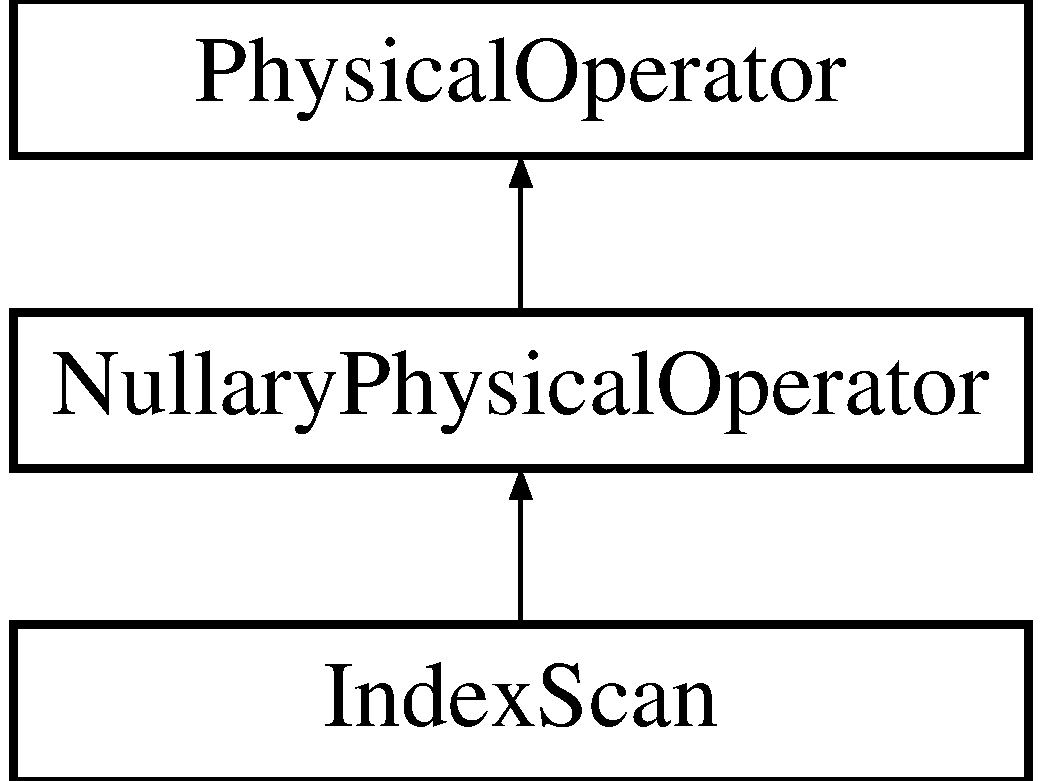
\includegraphics[height=3.000000cm]{class_index_scan}
\end{center}
\end{figure}
\subsection*{Public Member Functions}
\begin{DoxyCompactItemize}
\item 
\hyperlink{class_index_scan_a25eeb21a925a19209af7100de3f42ef5}{Index\+Scan} (const std\+::string \&name, const std\+::shared\+\_\+ptr$<$ \hyperlink{class_expression}{Expression} $>$ \&\hyperlink{class_index_scan_a9adcd1af97f3df02679f18fed687af21}{condition}, const \hyperlink{class_index}{Index} \&\hyperlink{class_index_scan_a8ffc3e0a33fb2db655471ea28e47bc9e}{index})
\item 
void \hyperlink{class_index_scan_a683950e9802678a2351f026ddb2a9881}{accept} (\hyperlink{class_physical_operator_visitor}{Physical\+Operator\+Visitor} \&v)
\end{DoxyCompactItemize}
\subsection*{Public Attributes}
\begin{DoxyCompactItemize}
\item 
std\+::string \hyperlink{class_index_scan_a8557a6ffee853f05298881acf8bebe14}{table\+Name}
\item 
std\+::shared\+\_\+ptr$<$ \hyperlink{class_expression}{Expression} $>$ \hyperlink{class_index_scan_a9adcd1af97f3df02679f18fed687af21}{condition}
\item 
\hyperlink{class_index}{Index} \hyperlink{class_index_scan_a8ffc3e0a33fb2db655471ea28e47bc9e}{index}
\end{DoxyCompactItemize}


\subsection{Detailed Description}
Represents operator, which reads part of the table using index. 

\subsection{Constructor \& Destructor Documentation}
\hypertarget{class_index_scan_a25eeb21a925a19209af7100de3f42ef5}{\index{Index\+Scan@{Index\+Scan}!Index\+Scan@{Index\+Scan}}
\index{Index\+Scan@{Index\+Scan}!Index\+Scan@{Index\+Scan}}
\subsubsection[{Index\+Scan}]{\setlength{\rightskip}{0pt plus 5cm}Index\+Scan\+::\+Index\+Scan (
\begin{DoxyParamCaption}
\item[{const std\+::string \&}]{name, }
\item[{const std\+::shared\+\_\+ptr$<$ {\bf Expression} $>$ \&}]{condition, }
\item[{const {\bf Index} \&}]{index}
\end{DoxyParamCaption}
)}}\label{class_index_scan_a25eeb21a925a19209af7100de3f42ef5}
Creates new instance of \hyperlink{class_index_scan}{Index\+Scan}. 
\begin{DoxyParams}{Parameters}
{\em name} & of table to read. \\
\hline
{\em condition} & to apply while reading. \\
\hline
{\em index} & -\/ index to user for reading. \\
\hline
\end{DoxyParams}


\subsection{Member Function Documentation}
\hypertarget{class_index_scan_a683950e9802678a2351f026ddb2a9881}{\index{Index\+Scan@{Index\+Scan}!accept@{accept}}
\index{accept@{accept}!Index\+Scan@{Index\+Scan}}
\subsubsection[{accept}]{\setlength{\rightskip}{0pt plus 5cm}void Index\+Scan\+::accept (
\begin{DoxyParamCaption}
\item[{{\bf Physical\+Operator\+Visitor} \&}]{v}
\end{DoxyParamCaption}
)\hspace{0.3cm}{\ttfamily [virtual]}}}\label{class_index_scan_a683950e9802678a2351f026ddb2a9881}
Method for calling visit\mbox{[}node\mbox{]} on given \hyperlink{class_physical_operator_visitor}{Physical\+Operator\+Visitor}. 
\begin{DoxyParams}{Parameters}
{\em v} & \hyperlink{class_physical_operator_visitor}{Physical\+Operator\+Visitor}, on which to call function. \\
\hline
\end{DoxyParams}


Implements \hyperlink{class_nullary_physical_operator_a053a51bc73b06d883fba982adeeb122c}{Nullary\+Physical\+Operator}.



\subsection{Member Data Documentation}
\hypertarget{class_index_scan_a9adcd1af97f3df02679f18fed687af21}{\index{Index\+Scan@{Index\+Scan}!condition@{condition}}
\index{condition@{condition}!Index\+Scan@{Index\+Scan}}
\subsubsection[{condition}]{\setlength{\rightskip}{0pt plus 5cm}std\+::shared\+\_\+ptr$<${\bf Expression}$>$ Index\+Scan\+::condition}}\label{class_index_scan_a9adcd1af97f3df02679f18fed687af21}
Condition to apply while reading. \hypertarget{class_index_scan_a8ffc3e0a33fb2db655471ea28e47bc9e}{\index{Index\+Scan@{Index\+Scan}!index@{index}}
\index{index@{index}!Index\+Scan@{Index\+Scan}}
\subsubsection[{index}]{\setlength{\rightskip}{0pt plus 5cm}{\bf Index} Index\+Scan\+::index}}\label{class_index_scan_a8ffc3e0a33fb2db655471ea28e47bc9e}
\hyperlink{class_table}{Table} index to use. \hypertarget{class_index_scan_a8557a6ffee853f05298881acf8bebe14}{\index{Index\+Scan@{Index\+Scan}!table\+Name@{table\+Name}}
\index{table\+Name@{table\+Name}!Index\+Scan@{Index\+Scan}}
\subsubsection[{table\+Name}]{\setlength{\rightskip}{0pt plus 5cm}std\+::string Index\+Scan\+::table\+Name}}\label{class_index_scan_a8557a6ffee853f05298881acf8bebe14}
\hyperlink{class_table}{Table} to read. 

The documentation for this class was generated from the following files\+:\begin{DoxyCompactItemize}
\item 
C\+:/\+Users/\+Marcel/\+Documents/\+Visual Studio 2012/\+Projects/\+Relational\+Query\+Evaluator/\+Relational\+Query\+Evaluator/Physical\+Operator.\+h\item 
C\+:/\+Users/\+Marcel/\+Documents/\+Visual Studio 2012/\+Projects/\+Relational\+Query\+Evaluator/\+Relational\+Query\+Evaluator/Physical\+Operator.\+cpp\end{DoxyCompactItemize}

\hypertarget{class_join}{\section{Join Class Reference}
\label{class_join}\index{Join@{Join}}
}
Inheritance diagram for Join\+:\begin{figure}[H]
\begin{center}
\leavevmode
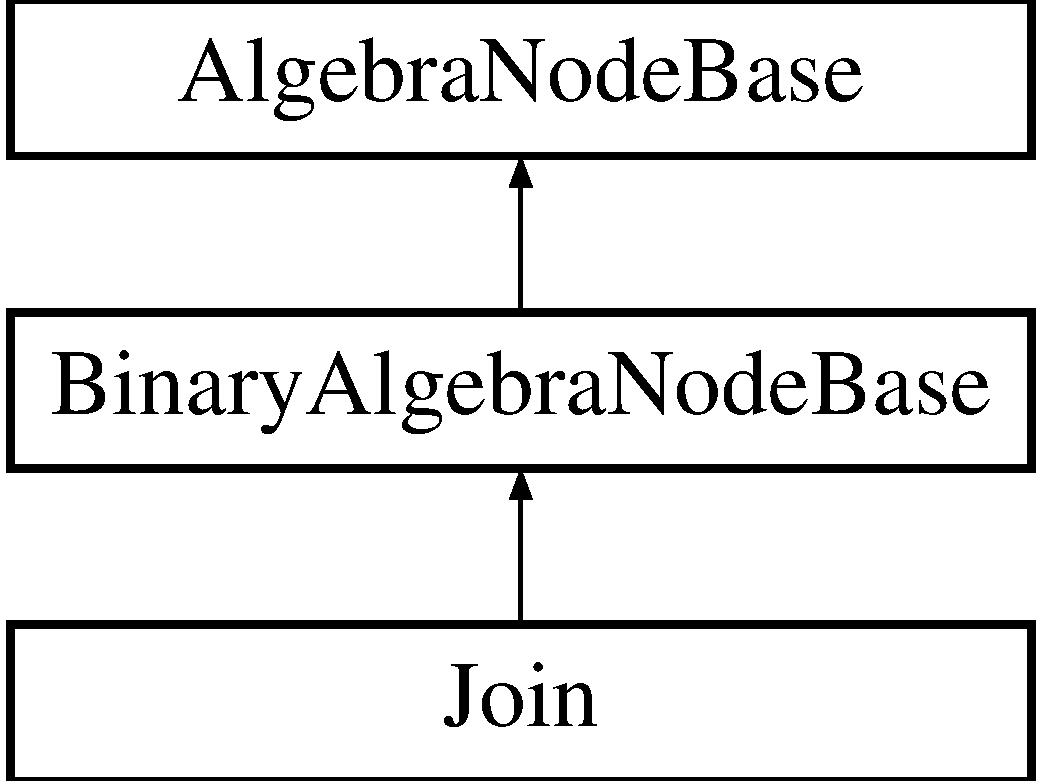
\includegraphics[height=3.000000cm]{class_join}
\end{center}
\end{figure}
\subsection*{Public Member Functions}
\begin{DoxyCompactItemize}
\item 
\hypertarget{class_join_ac9d8f69a2f72ce85df3e581292c46fc0}{{\bfseries Join} (D\+O\+M\+Element $\ast$element)}\label{class_join_ac9d8f69a2f72ce85df3e581292c46fc0}

\item 
\hypertarget{class_join_a387b23cf52fa9dc5390f003bcc051cc1}{void {\bfseries accept} (\hyperlink{class_algebra_visitor}{Algebra\+Visitor} \&v)}\label{class_join_a387b23cf52fa9dc5390f003bcc051cc1}

\end{DoxyCompactItemize}
\subsection*{Public Attributes}
\begin{DoxyCompactItemize}
\item 
\hypertarget{class_join_aa1374c434547d1a0a478a914ac0445bb}{std\+::shared\+\_\+ptr$<$ \hyperlink{class_expression}{Expression} $>$ {\bfseries condition}}\label{class_join_aa1374c434547d1a0a478a914ac0445bb}

\item 
\hypertarget{class_join_ad0fbf6166d055f84e2a1e9ec5af9824a}{std\+::vector$<$ \hyperlink{class_join_column_info}{Join\+Column\+Info} $>$ {\bfseries output\+Join\+Columns}}\label{class_join_ad0fbf6166d055f84e2a1e9ec5af9824a}

\end{DoxyCompactItemize}


The documentation for this class was generated from the following files\+:\begin{DoxyCompactItemize}
\item 
C\+:/\+Users/\+Marcel/\+Documents/\+Visual Studio 2012/\+Projects/\+Relational\+Query\+Evaluator/\+Relational\+Query\+Evaluator/Algebra.\+h\item 
C\+:/\+Users/\+Marcel/\+Documents/\+Visual Studio 2012/\+Projects/\+Relational\+Query\+Evaluator/\+Relational\+Query\+Evaluator/Algebra.\+cpp\end{DoxyCompactItemize}

\hypertarget{class_join_column_info}{\section{Join\+Column\+Info Class Reference}
\label{class_join_column_info}\index{Join\+Column\+Info@{Join\+Column\+Info}}
}
Inheritance diagram for Join\+Column\+Info\+:\begin{figure}[H]
\begin{center}
\leavevmode
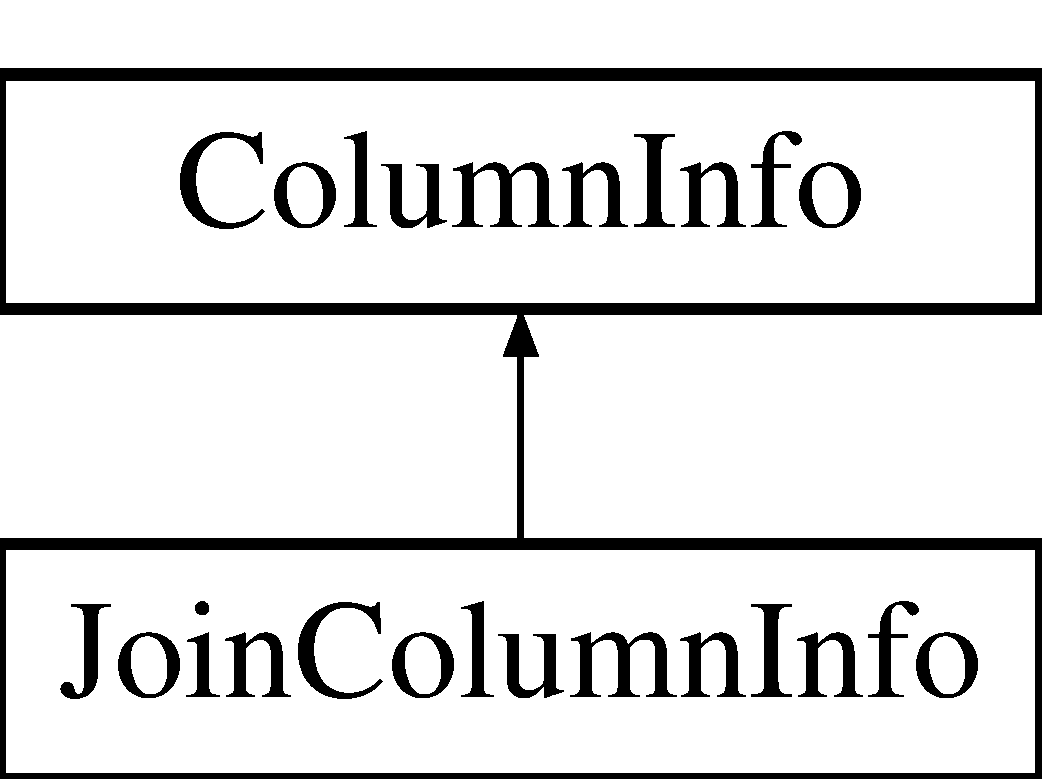
\includegraphics[height=2.000000cm]{class_join_column_info}
\end{center}
\end{figure}
\subsection*{Public Member Functions}
\begin{DoxyCompactItemize}
\item 
\hypertarget{class_join_column_info_a87471f04a13b3b2a5ff4bd60065e18d9}{{\bfseries Join\+Column\+Info} (const \hyperlink{class_column_info}{Column\+Info} \&col)}\label{class_join_column_info_a87471f04a13b3b2a5ff4bd60065e18d9}

\end{DoxyCompactItemize}
\subsection*{Public Attributes}
\begin{DoxyCompactItemize}
\item 
\hypertarget{class_join_column_info_a6a87e51d648e21dd6806d7a1bd6191da}{ulong {\bfseries input}}\label{class_join_column_info_a6a87e51d648e21dd6806d7a1bd6191da}

\item 
\hypertarget{class_join_column_info_a4fdb28a84e69012cdb314463f9c0d674}{std\+::string {\bfseries new\+Column}}\label{class_join_column_info_a4fdb28a84e69012cdb314463f9c0d674}

\end{DoxyCompactItemize}


The documentation for this class was generated from the following files\+:\begin{DoxyCompactItemize}
\item 
C\+:/\+Users/\+Marcel/\+Documents/\+Visual Studio 2012/\+Projects/\+Relational\+Query\+Evaluator/\+Relational\+Query\+Evaluator/Algebra\+Structures.\+h\item 
C\+:/\+Users/\+Marcel/\+Documents/\+Visual Studio 2012/\+Projects/\+Relational\+Query\+Evaluator/\+Relational\+Query\+Evaluator/Algebra\+Structures.\+cpp\end{DoxyCompactItemize}

\hypertarget{class_join_info}{\section{Join\+Info Class Reference}
\label{class_join_info}\index{Join\+Info@{Join\+Info}}
}


{\ttfamily \#include $<$Algebra\+Visitors.\+h$>$}

\subsection*{Public Member Functions}
\begin{DoxyCompactItemize}
\item 
void \hyperlink{class_join_info_aa4c03bd8c1d0a7f4a5b89287d69f89b5}{Remove\+Unnecessary\+Columns} (std\+::vector$<$ \hyperlink{class_join_column_info}{Join\+Column\+Info} $>$ \&output\+Columns)
\end{DoxyCompactItemize}
\subsection*{Static Public Member Functions}
\begin{DoxyCompactItemize}
\item 
static bool \hyperlink{class_join_info_ae7be09d7cdeb95ad59d9352ee37de990}{Comparator} (const std\+::shared\+\_\+ptr$<$ \hyperlink{class_join_info}{Join\+Info} $>$ \&lhs, const std\+::shared\+\_\+ptr$<$ \hyperlink{class_join_info}{Join\+Info} $>$ \&rhs)
\end{DoxyCompactItemize}
\subsection*{Public Attributes}
\begin{DoxyCompactItemize}
\item 
std\+::vector$<$ std\+::shared\+\_\+ptr\\*
$<$ \hyperlink{class_physical_plan}{Physical\+Plan} $>$ $>$ \hyperlink{class_join_info_acbddcf9cd01e91396492b94a627bdf69}{plans}
\item 
std\+::set$<$ ulong $>$ \hyperlink{class_join_info_a584f1ea54151c8e0c506911a6595c7cb}{processed\+Plans}
\item 
std\+::set$<$ ulong $>$ \hyperlink{class_join_info_ac6d0b302590c265ce7f3c47db28bad44}{un\+Processed\+Plans}
\item 
std\+::vector$<$ std\+::shared\+\_\+ptr\\*
$<$ \hyperlink{class_condition_info}{Condition\+Info} $>$ $>$ \hyperlink{class_join_info_a0b9f3b02df4e768208f53c549e0b6e61}{condition}
\item 
std\+::map$<$ ulong, \hyperlink{class_join_column_info}{Join\+Column\+Info} $>$ \hyperlink{class_join_info_a4890e0bbeaf9718d16765b8f408ec1b5}{columns}
\item 
double \hyperlink{class_join_info_a526146b07ef6d1bba7475f7998bf0588}{size}
\end{DoxyCompactItemize}


\subsection{Detailed Description}
Structures storing information in selecting join order algoritm. 

\subsection{Member Function Documentation}
\hypertarget{class_join_info_ae7be09d7cdeb95ad59d9352ee37de990}{\index{Join\+Info@{Join\+Info}!Comparator@{Comparator}}
\index{Comparator@{Comparator}!Join\+Info@{Join\+Info}}
\subsubsection[{Comparator}]{\setlength{\rightskip}{0pt plus 5cm}bool Join\+Info\+::\+Comparator (
\begin{DoxyParamCaption}
\item[{const std\+::shared\+\_\+ptr$<$ {\bf Join\+Info} $>$ \&}]{lhs, }
\item[{const std\+::shared\+\_\+ptr$<$ {\bf Join\+Info} $>$ \&}]{rhs}
\end{DoxyParamCaption}
)\hspace{0.3cm}{\ttfamily [static]}}}\label{class_join_info_ae7be09d7cdeb95ad59d9352ee37de990}
Comparer for head in greedy join order algorirthm. Compares plans bases on timecomplexity of plans\mbox{[}0\mbox{]}. Greedy join order algorirthm uses this structure with only one plan. 
\begin{DoxyParams}{Parameters}
{\em lhs} & -\/ first plan to compare \\
\hline
{\em rhs} & -\/ second plan to compare \\
\hline
\end{DoxyParams}
\begin{DoxyReturn}{Returns}
true if lsf is faster then rhs 
\end{DoxyReturn}
\hypertarget{class_join_info_aa4c03bd8c1d0a7f4a5b89287d69f89b5}{\index{Join\+Info@{Join\+Info}!Remove\+Unnecessary\+Columns@{Remove\+Unnecessary\+Columns}}
\index{Remove\+Unnecessary\+Columns@{Remove\+Unnecessary\+Columns}!Join\+Info@{Join\+Info}}
\subsubsection[{Remove\+Unnecessary\+Columns}]{\setlength{\rightskip}{0pt plus 5cm}void Join\+Info\+::\+Remove\+Unnecessary\+Columns (
\begin{DoxyParamCaption}
\item[{std\+::vector$<$ {\bf Join\+Column\+Info} $>$ \&}]{output\+Columns}
\end{DoxyParamCaption}
)}}\label{class_join_info_aa4c03bd8c1d0a7f4a5b89287d69f89b5}
Remove unecessary columns from current plans. Unnecessary columns are the one, which are not in condition out in output of procesed Group\+Join. 
\begin{DoxyParams}{Parameters}
{\em output\+Columns} & columns which are necessary. \\
\hline
\end{DoxyParams}


\subsection{Member Data Documentation}
\hypertarget{class_join_info_a4890e0bbeaf9718d16765b8f408ec1b5}{\index{Join\+Info@{Join\+Info}!columns@{columns}}
\index{columns@{columns}!Join\+Info@{Join\+Info}}
\subsubsection[{columns}]{\setlength{\rightskip}{0pt plus 5cm}std\+::map$<$ulong, {\bf Join\+Column\+Info}$>$ Join\+Info\+::columns}}\label{class_join_info_a4890e0bbeaf9718d16765b8f408ec1b5}
Output columns from current plans. \hypertarget{class_join_info_a0b9f3b02df4e768208f53c549e0b6e61}{\index{Join\+Info@{Join\+Info}!condition@{condition}}
\index{condition@{condition}!Join\+Info@{Join\+Info}}
\subsubsection[{condition}]{\setlength{\rightskip}{0pt plus 5cm}std\+::vector$<$std\+::shared\+\_\+ptr$<${\bf Condition\+Info}$>$ $>$ Join\+Info\+::condition}}\label{class_join_info_a0b9f3b02df4e768208f53c549e0b6e61}
Joiun condition to be processed. \hypertarget{class_join_info_acbddcf9cd01e91396492b94a627bdf69}{\index{Join\+Info@{Join\+Info}!plans@{plans}}
\index{plans@{plans}!Join\+Info@{Join\+Info}}
\subsubsection[{plans}]{\setlength{\rightskip}{0pt plus 5cm}std\+::vector$<$std\+::shared\+\_\+ptr$<${\bf Physical\+Plan}$>$ $>$ Join\+Info\+::plans}}\label{class_join_info_acbddcf9cd01e91396492b94a627bdf69}
Generated plans. \hypertarget{class_join_info_a584f1ea54151c8e0c506911a6595c7cb}{\index{Join\+Info@{Join\+Info}!processed\+Plans@{processed\+Plans}}
\index{processed\+Plans@{processed\+Plans}!Join\+Info@{Join\+Info}}
\subsubsection[{processed\+Plans}]{\setlength{\rightskip}{0pt plus 5cm}std\+::set$<$ulong$>$ Join\+Info\+::processed\+Plans}}\label{class_join_info_a584f1ea54151c8e0c506911a6595c7cb}
Numbers of processed inputs. \hypertarget{class_join_info_a526146b07ef6d1bba7475f7998bf0588}{\index{Join\+Info@{Join\+Info}!size@{size}}
\index{size@{size}!Join\+Info@{Join\+Info}}
\subsubsection[{size}]{\setlength{\rightskip}{0pt plus 5cm}double Join\+Info\+::size}}\label{class_join_info_a526146b07ef6d1bba7475f7998bf0588}
Size of the processed relation. \hypertarget{class_join_info_ac6d0b302590c265ce7f3c47db28bad44}{\index{Join\+Info@{Join\+Info}!un\+Processed\+Plans@{un\+Processed\+Plans}}
\index{un\+Processed\+Plans@{un\+Processed\+Plans}!Join\+Info@{Join\+Info}}
\subsubsection[{un\+Processed\+Plans}]{\setlength{\rightskip}{0pt plus 5cm}std\+::set$<$ulong$>$ Join\+Info\+::un\+Processed\+Plans}}\label{class_join_info_ac6d0b302590c265ce7f3c47db28bad44}
Numbers of unprocessed inputs. 

The documentation for this class was generated from the following files\+:\begin{DoxyCompactItemize}
\item 
C\+:/\+Users/\+Marcel/\+Documents/\+Visual Studio 2012/\+Projects/\+Relational\+Query\+Evaluator/\+Relational\+Query\+Evaluator/Algebra\+Visitors.\+h\item 
C\+:/\+Users/\+Marcel/\+Documents/\+Visual Studio 2012/\+Projects/\+Relational\+Query\+Evaluator/\+Relational\+Query\+Evaluator/Algebra\+Compiler.\+cpp\end{DoxyCompactItemize}

\hypertarget{class_join_info_reading_expression_visitor}{\section{Join\+Info\+Reading\+Expression\+Visitor Class Reference}
\label{class_join_info_reading_expression_visitor}\index{Join\+Info\+Reading\+Expression\+Visitor@{Join\+Info\+Reading\+Expression\+Visitor}}
}
Inheritance diagram for Join\+Info\+Reading\+Expression\+Visitor\+:\begin{figure}[H]
\begin{center}
\leavevmode
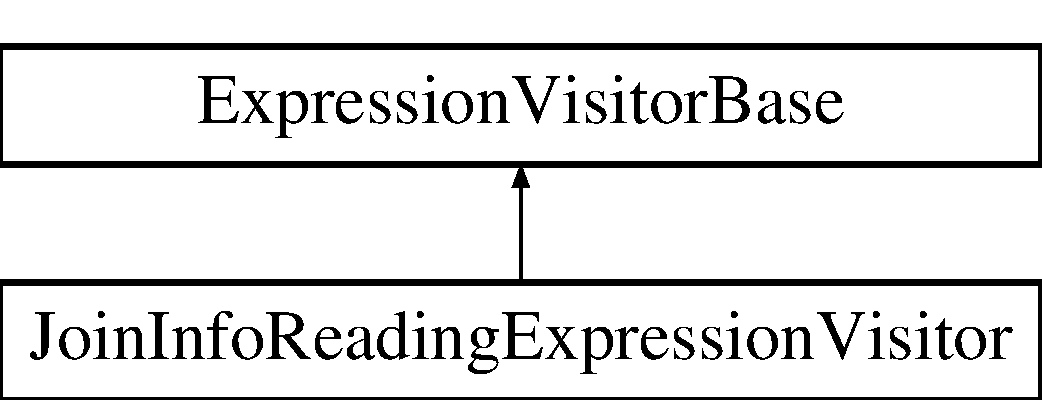
\includegraphics[height=2.000000cm]{class_join_info_reading_expression_visitor}
\end{center}
\end{figure}
\subsection*{Public Member Functions}
\begin{DoxyCompactItemize}
\item 
\hypertarget{class_join_info_reading_expression_visitor_a272a690d4b6ec6528a91f5ac0caae887}{{\bfseries Join\+Info\+Reading\+Expression\+Visitor} (std\+::set$<$ uint $>$ $\ast$data, Condition\+Type $\ast$type)}\label{class_join_info_reading_expression_visitor_a272a690d4b6ec6528a91f5ac0caae887}

\item 
\hypertarget{class_join_info_reading_expression_visitor_a03c3ec1bc690b6d9dc66a97efa75f2be}{void {\bfseries visit\+Column} (\hyperlink{class_column}{Column} $\ast$expression)}\label{class_join_info_reading_expression_visitor_a03c3ec1bc690b6d9dc66a97efa75f2be}

\item 
\hypertarget{class_join_info_reading_expression_visitor_a2254ead29d9226c771b530f43b677bd0}{void {\bfseries visit\+Unary\+Expression} (\hyperlink{class_unary_expression}{Unary\+Expression} $\ast$expression)}\label{class_join_info_reading_expression_visitor_a2254ead29d9226c771b530f43b677bd0}

\item 
\hypertarget{class_join_info_reading_expression_visitor_a6c6326b1ca8218ed35ac86ab7d487a0e}{void {\bfseries visit\+Binary\+Expression} (\hyperlink{class_binary_expression}{Binary\+Expression} $\ast$expression)}\label{class_join_info_reading_expression_visitor_a6c6326b1ca8218ed35ac86ab7d487a0e}

\item 
\hypertarget{class_join_info_reading_expression_visitor_a81cdbded017bc5e294b014122b94391c}{void {\bfseries visit\+Nnary\+Expression} (\hyperlink{class_nnary_expression}{Nnary\+Expression} $\ast$expression)}\label{class_join_info_reading_expression_visitor_a81cdbded017bc5e294b014122b94391c}

\item 
\hypertarget{class_join_info_reading_expression_visitor_a5d94ca3c0172aeaf3436fd15f3d9ba35}{void {\bfseries visit\+Constant} (\hyperlink{class_constant}{Constant} $\ast$expression)}\label{class_join_info_reading_expression_visitor_a5d94ca3c0172aeaf3436fd15f3d9ba35}

\item 
\hypertarget{class_join_info_reading_expression_visitor_af727a4e4a952f05080c8659ce0cff208}{void {\bfseries visit\+Grouped\+Expression} (\hyperlink{class_grouped_expression}{Grouped\+Expression} $\ast$expression)}\label{class_join_info_reading_expression_visitor_af727a4e4a952f05080c8659ce0cff208}

\end{DoxyCompactItemize}
\subsection*{Public Attributes}
\begin{DoxyCompactItemize}
\item 
\hypertarget{class_join_info_reading_expression_visitor_aa74d0cd4070b81c0eb6bf5870fa000d3}{std\+::set$<$ uint $>$ $\ast$ {\bfseries data}}\label{class_join_info_reading_expression_visitor_aa74d0cd4070b81c0eb6bf5870fa000d3}

\item 
\hypertarget{class_join_info_reading_expression_visitor_af7219e9cb55b9a59763a06df0656a63f}{Condition\+Type $\ast$ {\bfseries condition\+Type}}\label{class_join_info_reading_expression_visitor_af7219e9cb55b9a59763a06df0656a63f}

\end{DoxyCompactItemize}


The documentation for this class was generated from the following file\+:\begin{DoxyCompactItemize}
\item 
C\+:/\+Users/\+Marcel/\+Documents/\+Visual Studio 2012/\+Projects/\+Relational\+Query\+Evaluator/\+Relational\+Query\+Evaluator/Expression\+Visitors.\+h\end{DoxyCompactItemize}

\hypertarget{class_max_of_unique_values_expression_visitor}{\section{Max\+Of\+Unique\+Values\+Expression\+Visitor Class Reference}
\label{class_max_of_unique_values_expression_visitor}\index{Max\+Of\+Unique\+Values\+Expression\+Visitor@{Max\+Of\+Unique\+Values\+Expression\+Visitor}}
}
Inheritance diagram for Max\+Of\+Unique\+Values\+Expression\+Visitor\+:\begin{figure}[H]
\begin{center}
\leavevmode
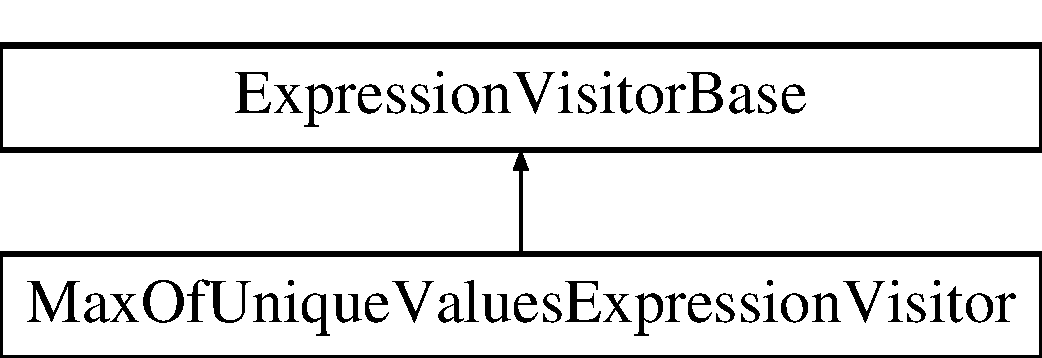
\includegraphics[height=2.000000cm]{class_max_of_unique_values_expression_visitor}
\end{center}
\end{figure}
\subsection*{Public Member Functions}
\begin{DoxyCompactItemize}
\item 
\hypertarget{class_max_of_unique_values_expression_visitor_adf863a6e2406f90466e4f4decab1f4e4}{{\bfseries Max\+Of\+Unique\+Values\+Expression\+Visitor} (std\+::map$<$ int, \hyperlink{class_column_info}{Column\+Info} $>$ $\ast$cols)}\label{class_max_of_unique_values_expression_visitor_adf863a6e2406f90466e4f4decab1f4e4}

\item 
void \hyperlink{class_max_of_unique_values_expression_visitor_a1e924d4d6d63474f401adc0c8ba6a455}{visit\+Column} (\hyperlink{class_column}{Column} $\ast$expression)
\end{DoxyCompactItemize}
\subsection*{Public Attributes}
\begin{DoxyCompactItemize}
\item 
\hypertarget{class_max_of_unique_values_expression_visitor_a4d1359a778ac14a3709c63bff3a01383}{double {\bfseries result}}\label{class_max_of_unique_values_expression_visitor_a4d1359a778ac14a3709c63bff3a01383}

\item 
\hypertarget{class_max_of_unique_values_expression_visitor_a1f0ca5cd4e5fd0eb513fa64ea21ecae6}{std\+::map$<$ int, \hyperlink{class_column_info}{Column\+Info} $>$ $\ast$ {\bfseries columns}}\label{class_max_of_unique_values_expression_visitor_a1f0ca5cd4e5fd0eb513fa64ea21ecae6}

\end{DoxyCompactItemize}


\subsection{Member Function Documentation}
\hypertarget{class_max_of_unique_values_expression_visitor_a1e924d4d6d63474f401adc0c8ba6a455}{\index{Max\+Of\+Unique\+Values\+Expression\+Visitor@{Max\+Of\+Unique\+Values\+Expression\+Visitor}!visit\+Column@{visit\+Column}}
\index{visit\+Column@{visit\+Column}!Max\+Of\+Unique\+Values\+Expression\+Visitor@{Max\+Of\+Unique\+Values\+Expression\+Visitor}}
\subsubsection[{visit\+Column}]{\setlength{\rightskip}{0pt plus 5cm}void Max\+Of\+Unique\+Values\+Expression\+Visitor\+::visit\+Column (
\begin{DoxyParamCaption}
\item[{{\bf Column} $\ast$}]{expression}
\end{DoxyParamCaption}
)\hspace{0.3cm}{\ttfamily [virtual]}}}\label{class_max_of_unique_values_expression_visitor_a1e924d4d6d63474f401adc0c8ba6a455}
Visits \hyperlink{class_column}{Column} element. 
\begin{DoxyParams}{Parameters}
{\em expression} & visited \hyperlink{class_column}{Column}. \\
\hline
\end{DoxyParams}


Reimplemented from \hyperlink{class_expression_visitor_base_a1ac638b82248ff9e1582dbf520dc6ae4}{Expression\+Visitor\+Base}.



The documentation for this class was generated from the following files\+:\begin{DoxyCompactItemize}
\item 
C\+:/\+Users/\+Marcel/\+Documents/\+Visual Studio 2012/\+Projects/\+Relational\+Query\+Evaluator/\+Relational\+Query\+Evaluator/Expression\+Visitors.\+h\item 
C\+:/\+Users/\+Marcel/\+Documents/\+Visual Studio 2012/\+Projects/\+Relational\+Query\+Evaluator/\+Relational\+Query\+Evaluator/Expression\+Visitors.\+cpp\end{DoxyCompactItemize}

\hypertarget{class_merge_anti_join}{\section{Merge\+Anti\+Join Class Reference}
\label{class_merge_anti_join}\index{Merge\+Anti\+Join@{Merge\+Anti\+Join}}
}
Inheritance diagram for Merge\+Anti\+Join\+:\begin{figure}[H]
\begin{center}
\leavevmode
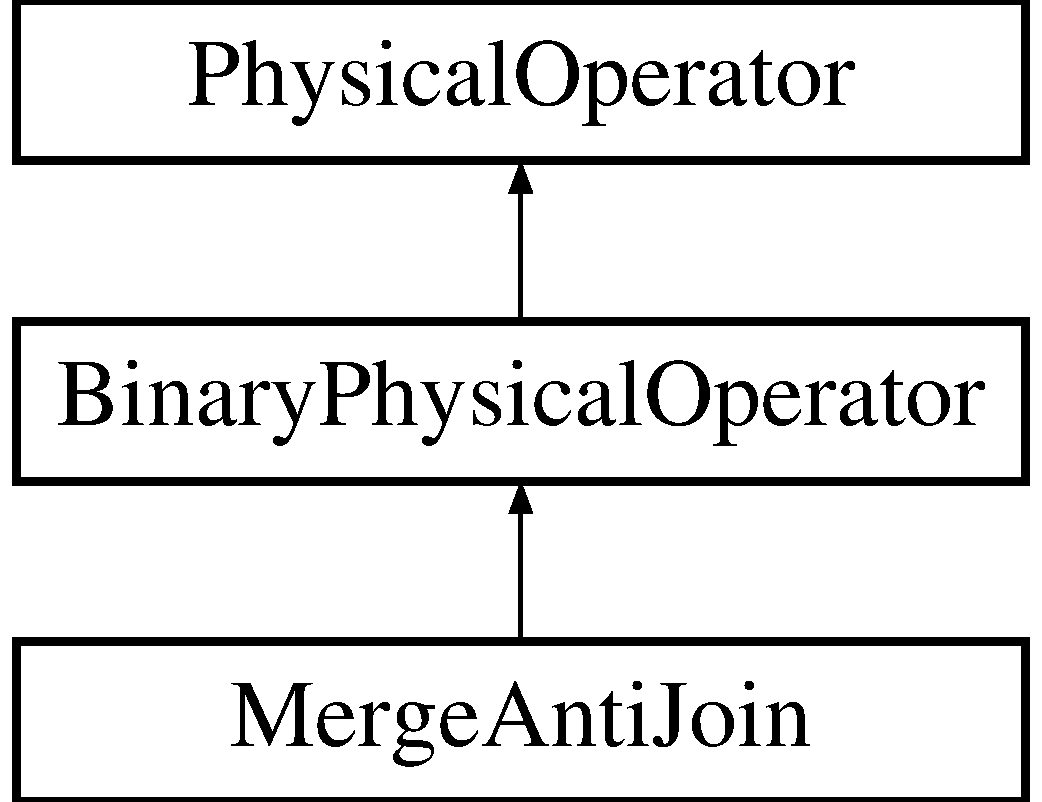
\includegraphics[height=3.000000cm]{class_merge_anti_join}
\end{center}
\end{figure}
\subsection*{Public Member Functions}
\begin{DoxyCompactItemize}
\item 
\hypertarget{class_merge_anti_join_a314a1c84c2b6c6848f5f4664c2b13c77}{{\bfseries Merge\+Anti\+Join} (const std\+::shared\+\_\+ptr$<$ \hyperlink{class_expression}{Expression} $>$ \&condition)}\label{class_merge_anti_join_a314a1c84c2b6c6848f5f4664c2b13c77}

\item 
\hypertarget{class_merge_anti_join_a15758e7f808703b243101faa382a0156}{void {\bfseries accept} (\hyperlink{class_physical_operator_visitor}{Physical\+Operator\+Visitor} \&v)}\label{class_merge_anti_join_a15758e7f808703b243101faa382a0156}

\end{DoxyCompactItemize}
\subsection*{Public Attributes}
\begin{DoxyCompactItemize}
\item 
\hypertarget{class_merge_anti_join_ae616cc88814ffd21b31ed48693ac60a6}{std\+::shared\+\_\+ptr$<$ \hyperlink{class_expression}{Expression} $>$ {\bfseries condition}}\label{class_merge_anti_join_ae616cc88814ffd21b31ed48693ac60a6}

\item 
\hypertarget{class_merge_anti_join_a1dedfa039b1172db367fc7d3cd0304fc}{std\+::vector$<$ \hyperlink{class_sort_parameter}{Sort\+Parameter} $>$ {\bfseries left}}\label{class_merge_anti_join_a1dedfa039b1172db367fc7d3cd0304fc}

\item 
\hypertarget{class_merge_anti_join_a28f20cf708052a9357799187831c8a33}{std\+::vector$<$ \hyperlink{class_sort_parameter}{Sort\+Parameter} $>$ {\bfseries right}}\label{class_merge_anti_join_a28f20cf708052a9357799187831c8a33}

\end{DoxyCompactItemize}


The documentation for this class was generated from the following files\+:\begin{DoxyCompactItemize}
\item 
C\+:/\+Users/\+Marcel/\+Documents/\+Visual Studio 2012/\+Projects/\+Relational\+Query\+Evaluator/\+Relational\+Query\+Evaluator/Physical\+Operator.\+h\item 
C\+:/\+Users/\+Marcel/\+Documents/\+Visual Studio 2012/\+Projects/\+Relational\+Query\+Evaluator/\+Relational\+Query\+Evaluator/Physical\+Operator.\+cpp\end{DoxyCompactItemize}

\hypertarget{class_merge_equi_join}{\section{Merge\+Equi\+Join Class Reference}
\label{class_merge_equi_join}\index{Merge\+Equi\+Join@{Merge\+Equi\+Join}}
}


{\ttfamily \#include $<$Physical\+Operator.\+h$>$}

Inheritance diagram for Merge\+Equi\+Join\+:\begin{figure}[H]
\begin{center}
\leavevmode
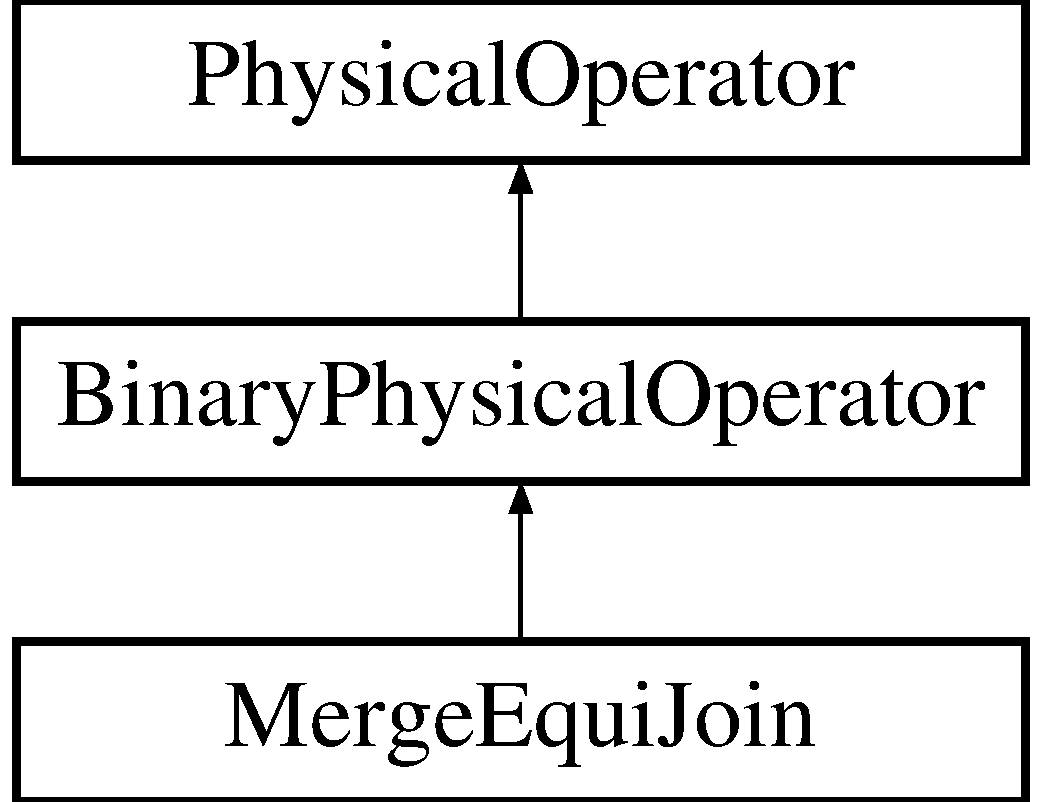
\includegraphics[height=3.000000cm]{class_merge_equi_join}
\end{center}
\end{figure}
\subsection*{Public Member Functions}
\begin{DoxyCompactItemize}
\item 
\hyperlink{class_merge_equi_join_a16fa9f23ebbd531c398b121a99c18afc}{Merge\+Equi\+Join} (const std\+::shared\+\_\+ptr$<$ \hyperlink{class_expression}{Expression} $>$ \&\hyperlink{class_merge_equi_join_ac334a1377a90c2876f9a5fad38d1836e}{condition})
\item 
void \hyperlink{class_merge_equi_join_a0a88e744444a5a539d58aac25c609a9c}{accept} (\hyperlink{class_physical_operator_visitor}{Physical\+Operator\+Visitor} \&v)
\end{DoxyCompactItemize}
\subsection*{Public Attributes}
\begin{DoxyCompactItemize}
\item 
std\+::shared\+\_\+ptr$<$ \hyperlink{class_expression}{Expression} $>$ \hyperlink{class_merge_equi_join_ac334a1377a90c2876f9a5fad38d1836e}{condition}
\item 
std\+::vector$<$ \hyperlink{class_sort_parameter}{Sort\+Parameter} $>$ \hyperlink{class_merge_equi_join_a10a2e1737a5d7c2e554f55b0e0863d04}{left}
\item 
std\+::vector$<$ \hyperlink{class_sort_parameter}{Sort\+Parameter} $>$ \hyperlink{class_merge_equi_join_a0d32b50a198ce479cae3bbdc52b9766a}{right}
\end{DoxyCompactItemize}


\subsection{Detailed Description}
Represents merge equi join. Operator computes equijoin from given sorted inputs. 

\subsection{Constructor \& Destructor Documentation}
\hypertarget{class_merge_equi_join_a16fa9f23ebbd531c398b121a99c18afc}{\index{Merge\+Equi\+Join@{Merge\+Equi\+Join}!Merge\+Equi\+Join@{Merge\+Equi\+Join}}
\index{Merge\+Equi\+Join@{Merge\+Equi\+Join}!Merge\+Equi\+Join@{Merge\+Equi\+Join}}
\subsubsection[{Merge\+Equi\+Join}]{\setlength{\rightskip}{0pt plus 5cm}Merge\+Equi\+Join\+::\+Merge\+Equi\+Join (
\begin{DoxyParamCaption}
\item[{const std\+::shared\+\_\+ptr$<$ {\bf Expression} $>$ \&}]{condition}
\end{DoxyParamCaption}
)}}\label{class_merge_equi_join_a16fa9f23ebbd531c398b121a99c18afc}
Creates new instance of \hyperlink{class_merge_equi_join}{Merge\+Equi\+Join}. 
\begin{DoxyParams}{Parameters}
{\em condition} & -\/ join condition. \\
\hline
\end{DoxyParams}


\subsection{Member Function Documentation}
\hypertarget{class_merge_equi_join_a0a88e744444a5a539d58aac25c609a9c}{\index{Merge\+Equi\+Join@{Merge\+Equi\+Join}!accept@{accept}}
\index{accept@{accept}!Merge\+Equi\+Join@{Merge\+Equi\+Join}}
\subsubsection[{accept}]{\setlength{\rightskip}{0pt plus 5cm}void Merge\+Equi\+Join\+::accept (
\begin{DoxyParamCaption}
\item[{{\bf Physical\+Operator\+Visitor} \&}]{v}
\end{DoxyParamCaption}
)\hspace{0.3cm}{\ttfamily [virtual]}}}\label{class_merge_equi_join_a0a88e744444a5a539d58aac25c609a9c}
Method for calling visit\mbox{[}node\mbox{]} on given \hyperlink{class_physical_operator_visitor}{Physical\+Operator\+Visitor}. 
\begin{DoxyParams}{Parameters}
{\em v} & \hyperlink{class_physical_operator_visitor}{Physical\+Operator\+Visitor}, on which to call function. \\
\hline
\end{DoxyParams}


Implements \hyperlink{class_binary_physical_operator_a29ec622920006cb5428bf2c259918347}{Binary\+Physical\+Operator}.



\subsection{Member Data Documentation}
\hypertarget{class_merge_equi_join_ac334a1377a90c2876f9a5fad38d1836e}{\index{Merge\+Equi\+Join@{Merge\+Equi\+Join}!condition@{condition}}
\index{condition@{condition}!Merge\+Equi\+Join@{Merge\+Equi\+Join}}
\subsubsection[{condition}]{\setlength{\rightskip}{0pt plus 5cm}std\+::shared\+\_\+ptr$<${\bf Expression}$>$ Merge\+Equi\+Join\+::condition}}\label{class_merge_equi_join_ac334a1377a90c2876f9a5fad38d1836e}
\hyperlink{class_join}{Join} condition. \hypertarget{class_merge_equi_join_a10a2e1737a5d7c2e554f55b0e0863d04}{\index{Merge\+Equi\+Join@{Merge\+Equi\+Join}!left@{left}}
\index{left@{left}!Merge\+Equi\+Join@{Merge\+Equi\+Join}}
\subsubsection[{left}]{\setlength{\rightskip}{0pt plus 5cm}std\+::vector$<${\bf Sort\+Parameter}$>$ Merge\+Equi\+Join\+::left}}\label{class_merge_equi_join_a10a2e1737a5d7c2e554f55b0e0863d04}
Stored information how first input is sorted. \hypertarget{class_merge_equi_join_a0d32b50a198ce479cae3bbdc52b9766a}{\index{Merge\+Equi\+Join@{Merge\+Equi\+Join}!right@{right}}
\index{right@{right}!Merge\+Equi\+Join@{Merge\+Equi\+Join}}
\subsubsection[{right}]{\setlength{\rightskip}{0pt plus 5cm}std\+::vector$<${\bf Sort\+Parameter}$>$ Merge\+Equi\+Join\+::right}}\label{class_merge_equi_join_a0d32b50a198ce479cae3bbdc52b9766a}
Stored information how second input is sorted. 

The documentation for this class was generated from the following files\+:\begin{DoxyCompactItemize}
\item 
C\+:/\+Users/\+Marcel/\+Documents/\+Visual Studio 2012/\+Projects/\+Relational\+Query\+Evaluator/\+Relational\+Query\+Evaluator/Physical\+Operator.\+h\item 
C\+:/\+Users/\+Marcel/\+Documents/\+Visual Studio 2012/\+Projects/\+Relational\+Query\+Evaluator/\+Relational\+Query\+Evaluator/Physical\+Operator.\+cpp\end{DoxyCompactItemize}

\hypertarget{class_merge_non_equi_join}{\section{Merge\+Non\+Equi\+Join Class Reference}
\label{class_merge_non_equi_join}\index{Merge\+Non\+Equi\+Join@{Merge\+Non\+Equi\+Join}}
}
Inheritance diagram for Merge\+Non\+Equi\+Join\+:\begin{figure}[H]
\begin{center}
\leavevmode
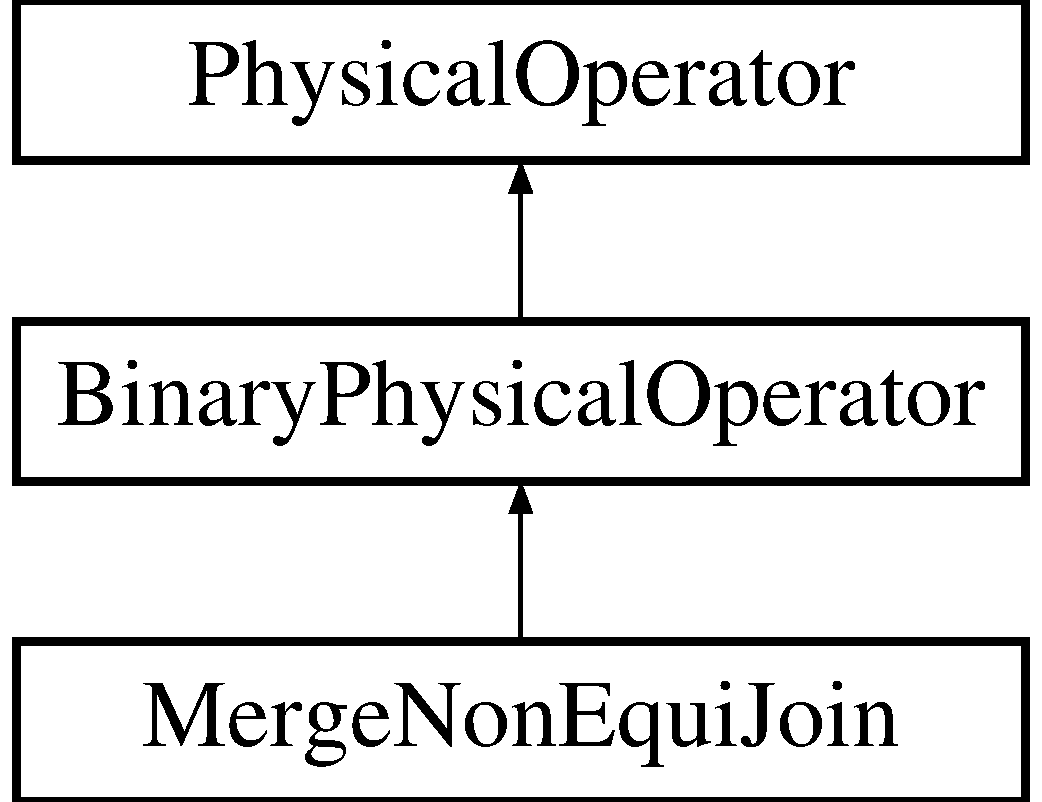
\includegraphics[height=3.000000cm]{class_merge_non_equi_join}
\end{center}
\end{figure}
\subsection*{Public Member Functions}
\begin{DoxyCompactItemize}
\item 
\hypertarget{class_merge_non_equi_join_a117ec79e9941977b4f90c65bea5cea65}{void {\bfseries accept} (\hyperlink{class_physical_operator_visitor}{Physical\+Operator\+Visitor} \&v)}\label{class_merge_non_equi_join_a117ec79e9941977b4f90c65bea5cea65}

\item 
\hypertarget{class_merge_non_equi_join_a3e7a12e0e21a2bf755608c9bc2e5d4ed}{{\bfseries Merge\+Non\+Equi\+Join} (const std\+::shared\+\_\+ptr$<$ \hyperlink{class_expression}{Expression} $>$ \&condition)}\label{class_merge_non_equi_join_a3e7a12e0e21a2bf755608c9bc2e5d4ed}

\end{DoxyCompactItemize}
\subsection*{Public Attributes}
\begin{DoxyCompactItemize}
\item 
\hypertarget{class_merge_non_equi_join_ad1307cbe8f5e88f685ece833fcea67c2}{std\+::shared\+\_\+ptr$<$ \hyperlink{class_expression}{Expression} $>$ {\bfseries condition}}\label{class_merge_non_equi_join_ad1307cbe8f5e88f685ece833fcea67c2}

\item 
\hypertarget{class_merge_non_equi_join_a5f8b68c20d65ec2e07f41f2c2c4079d6}{std\+::vector$<$ \hyperlink{class_sort_parameter}{Sort\+Parameter} $>$ {\bfseries sort\+Parameters}}\label{class_merge_non_equi_join_a5f8b68c20d65ec2e07f41f2c2c4079d6}

\item 
\hypertarget{class_merge_non_equi_join_a785b0aeaa5ec15536c03272a21f8ebe0}{std\+::vector$<$ \hyperlink{class_sort_parameter}{Sort\+Parameter} $>$ {\bfseries left}}\label{class_merge_non_equi_join_a785b0aeaa5ec15536c03272a21f8ebe0}

\item 
\hypertarget{class_merge_non_equi_join_ae3631adf9752e5ab861dbf986b92ff00}{std\+::vector$<$ \hyperlink{class_sort_parameter}{Sort\+Parameter} $>$ {\bfseries right}}\label{class_merge_non_equi_join_ae3631adf9752e5ab861dbf986b92ff00}

\end{DoxyCompactItemize}


The documentation for this class was generated from the following files\+:\begin{DoxyCompactItemize}
\item 
C\+:/\+Users/\+Marcel/\+Documents/\+Visual Studio 2012/\+Projects/\+Relational\+Query\+Evaluator/\+Relational\+Query\+Evaluator/Physical\+Operator.\+h\item 
C\+:/\+Users/\+Marcel/\+Documents/\+Visual Studio 2012/\+Projects/\+Relational\+Query\+Evaluator/\+Relational\+Query\+Evaluator/Physical\+Operator.\+cpp\end{DoxyCompactItemize}

\hypertarget{class_nnary_expression}{\section{Nnary\+Expression Class Reference}
\label{class_nnary_expression}\index{Nnary\+Expression@{Nnary\+Expression}}
}


{\ttfamily \#include $<$Expressions.\+h$>$}

Inheritance diagram for Nnary\+Expression\+:\begin{figure}[H]
\begin{center}
\leavevmode
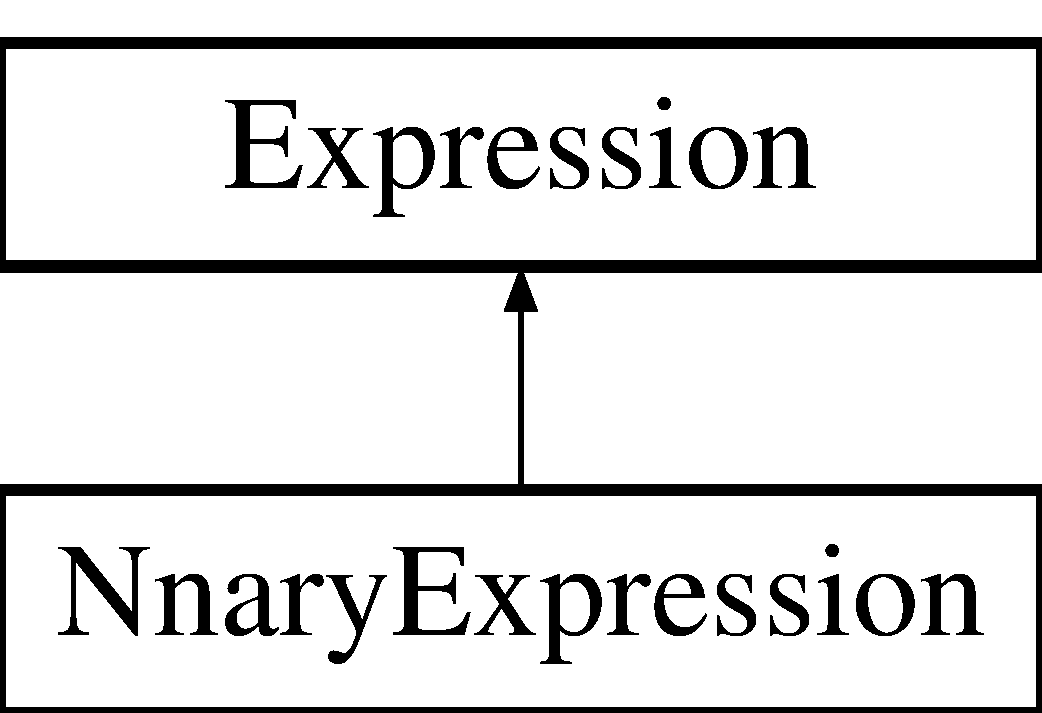
\includegraphics[height=2.000000cm]{class_nnary_expression}
\end{center}
\end{figure}
\subsection*{Public Member Functions}
\begin{DoxyCompactItemize}
\item 
\hyperlink{class_nnary_expression_a38f44966213fd5d674aaff3ef9de37da}{Nnary\+Expression} (D\+O\+M\+Element $\ast$node, const std\+::string \&\hyperlink{class_nnary_expression_ab21462327a70e8955c74cd8cc3fc428f}{name}, const std\+::string \&\hyperlink{class_nnary_expression_a70b8058f410ed9f52b610e74489bf03f}{return\+Type})
\item 
void \hyperlink{class_nnary_expression_a5934f3925e13888b3241f6b269d5ee44}{accept} (\hyperlink{class_expression_visitor_base}{Expression\+Visitor\+Base} \&v)
\item 
void \hyperlink{class_nnary_expression_a1161a6f8776c4cc946d769e4526339a2}{replace\+Child} (\hyperlink{class_expression}{Expression} $\ast$old\+Child, std\+::shared\+\_\+ptr$<$ \hyperlink{class_expression}{Expression} $>$ new\+Child)
\end{DoxyCompactItemize}
\subsection*{Public Attributes}
\begin{DoxyCompactItemize}
\item 
std\+::string \hyperlink{class_nnary_expression_ab21462327a70e8955c74cd8cc3fc428f}{name}
\item 
std\+::string \hyperlink{class_nnary_expression_a70b8058f410ed9f52b610e74489bf03f}{return\+Type}
\item 
std\+::vector$<$ std\+::shared\+\_\+ptr\\*
$<$ \hyperlink{class_expression}{Expression} $>$ $>$ \hyperlink{class_nnary_expression_ae70d24059bba49f089137557e18f41a9}{arguments}
\end{DoxyCompactItemize}
\subsection*{Additional Inherited Members}


\subsection{Detailed Description}
Represents co called n-\/nary expresion, it is a function call with variable argument number. N-\/nary expression can be for expample sql function like or date or arithmetic function sqrt 

\subsection{Constructor \& Destructor Documentation}
\hypertarget{class_nnary_expression_a38f44966213fd5d674aaff3ef9de37da}{\index{Nnary\+Expression@{Nnary\+Expression}!Nnary\+Expression@{Nnary\+Expression}}
\index{Nnary\+Expression@{Nnary\+Expression}!Nnary\+Expression@{Nnary\+Expression}}
\subsubsection[{Nnary\+Expression}]{\setlength{\rightskip}{0pt plus 5cm}Nnary\+Expression\+::\+Nnary\+Expression (
\begin{DoxyParamCaption}
\item[{D\+O\+M\+Element $\ast$}]{node, }
\item[{const std\+::string \&}]{name, }
\item[{const std\+::string \&}]{return\+Type}
\end{DoxyParamCaption}
)}}\label{class_nnary_expression_a38f44966213fd5d674aaff3ef9de37da}
Creates new instace of \hyperlink{class_nnary_expression}{Nnary\+Expression}. 
\begin{DoxyParams}{Parameters}
{\em node} & -\/ element containing infromation about node and it's children \\
\hline
{\em name} & -\/ function name \\
\hline
{\em return\+Type} & -\/ return type of function \\
\hline
\end{DoxyParams}


\subsection{Member Function Documentation}
\hypertarget{class_nnary_expression_a5934f3925e13888b3241f6b269d5ee44}{\index{Nnary\+Expression@{Nnary\+Expression}!accept@{accept}}
\index{accept@{accept}!Nnary\+Expression@{Nnary\+Expression}}
\subsubsection[{accept}]{\setlength{\rightskip}{0pt plus 5cm}void Nnary\+Expression\+::accept (
\begin{DoxyParamCaption}
\item[{{\bf Expression\+Visitor\+Base} \&}]{v}
\end{DoxyParamCaption}
)\hspace{0.3cm}{\ttfamily [virtual]}}}\label{class_nnary_expression_a5934f3925e13888b3241f6b269d5ee44}
Method for calling visit\mbox{[}node\mbox{]} on given Expression\+Visitor 
\begin{DoxyParams}{Parameters}
{\em v} & Expression\+Visitor, on which to call visit function \\
\hline
\end{DoxyParams}


Implements \hyperlink{class_expression_ae2e6c802668a6329658b7c982f9c7b33}{Expression}.

\hypertarget{class_nnary_expression_a1161a6f8776c4cc946d769e4526339a2}{\index{Nnary\+Expression@{Nnary\+Expression}!replace\+Child@{replace\+Child}}
\index{replace\+Child@{replace\+Child}!Nnary\+Expression@{Nnary\+Expression}}
\subsubsection[{replace\+Child}]{\setlength{\rightskip}{0pt plus 5cm}void Nnary\+Expression\+::replace\+Child (
\begin{DoxyParamCaption}
\item[{{\bf Expression} $\ast$}]{old\+Child, }
\item[{std\+::shared\+\_\+ptr$<$ {\bf Expression} $>$}]{new\+Child}
\end{DoxyParamCaption}
)\hspace{0.3cm}{\ttfamily [virtual]}}}\label{class_nnary_expression_a1161a6f8776c4cc946d769e4526339a2}
Replaces child from this class with new expression tree. 
\begin{DoxyParams}{Parameters}
{\em old\+Child} & -\/ child to replace \\
\hline
{\em new\+Child} & -\/ child to be replaced \\
\hline
\end{DoxyParams}


Implements \hyperlink{class_expression_a77ac16bbb0df93de8a7711b2f7de889f}{Expression}.



\subsection{Member Data Documentation}
\hypertarget{class_nnary_expression_ae70d24059bba49f089137557e18f41a9}{\index{Nnary\+Expression@{Nnary\+Expression}!arguments@{arguments}}
\index{arguments@{arguments}!Nnary\+Expression@{Nnary\+Expression}}
\subsubsection[{arguments}]{\setlength{\rightskip}{0pt plus 5cm}std\+::vector$<$std\+::shared\+\_\+ptr$<${\bf Expression}$>$ $>$ Nnary\+Expression\+::arguments}}\label{class_nnary_expression_ae70d24059bba49f089137557e18f41a9}
Stores call arguments. Arguments are also expression trees. \hypertarget{class_nnary_expression_ab21462327a70e8955c74cd8cc3fc428f}{\index{Nnary\+Expression@{Nnary\+Expression}!name@{name}}
\index{name@{name}!Nnary\+Expression@{Nnary\+Expression}}
\subsubsection[{name}]{\setlength{\rightskip}{0pt plus 5cm}std\+::string Nnary\+Expression\+::name}}\label{class_nnary_expression_ab21462327a70e8955c74cd8cc3fc428f}
Stores function name. \hypertarget{class_nnary_expression_a70b8058f410ed9f52b610e74489bf03f}{\index{Nnary\+Expression@{Nnary\+Expression}!return\+Type@{return\+Type}}
\index{return\+Type@{return\+Type}!Nnary\+Expression@{Nnary\+Expression}}
\subsubsection[{return\+Type}]{\setlength{\rightskip}{0pt plus 5cm}std\+::string Nnary\+Expression\+::return\+Type}}\label{class_nnary_expression_a70b8058f410ed9f52b610e74489bf03f}
Stores function return type. 

The documentation for this class was generated from the following files\+:\begin{DoxyCompactItemize}
\item 
C\+:/\+Users/\+Marcel/\+Documents/\+Visual Studio 2012/\+Projects/\+Relational\+Query\+Evaluator/\+Relational\+Query\+Evaluator/Expressions.\+h\item 
C\+:/\+Users/\+Marcel/\+Documents/\+Visual Studio 2012/\+Projects/\+Relational\+Query\+Evaluator/\+Relational\+Query\+Evaluator/Expressions.\+cpp\end{DoxyCompactItemize}

\hypertarget{class_nullary_algebra_node_base}{\section{Nullary\+Algebra\+Node\+Base Class Reference}
\label{class_nullary_algebra_node_base}\index{Nullary\+Algebra\+Node\+Base@{Nullary\+Algebra\+Node\+Base}}
}


{\ttfamily \#include $<$Algebra.\+h$>$}

Inheritance diagram for Nullary\+Algebra\+Node\+Base\+:\begin{figure}[H]
\begin{center}
\leavevmode
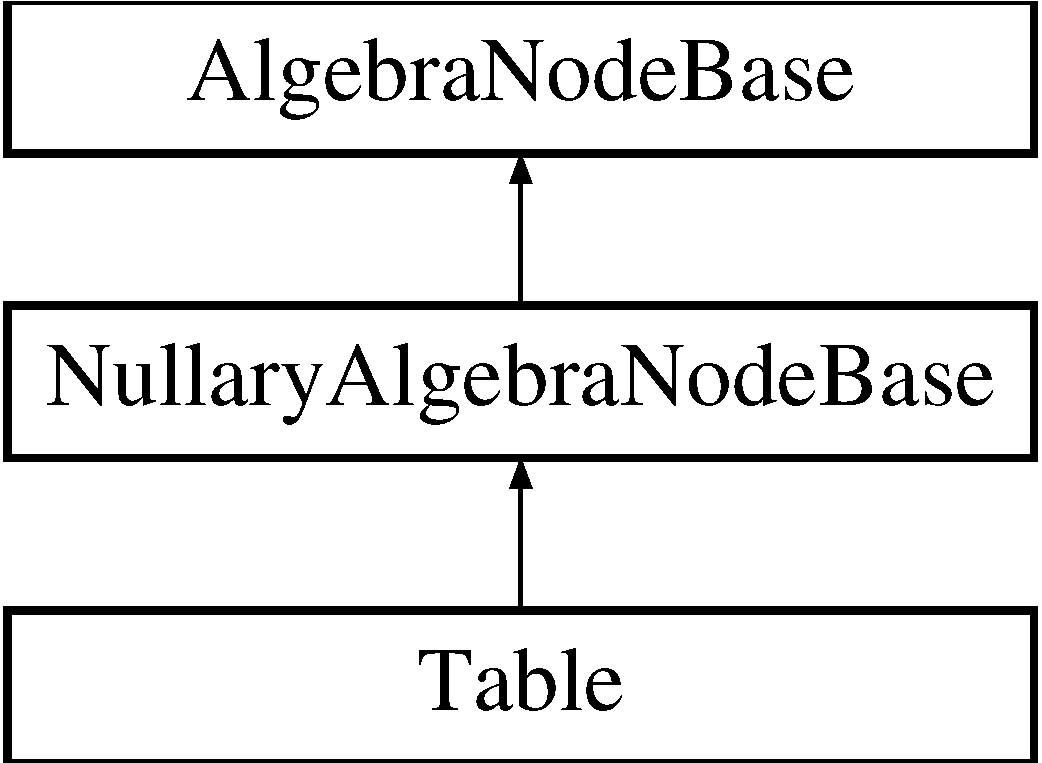
\includegraphics[height=3.000000cm]{class_nullary_algebra_node_base}
\end{center}
\end{figure}
\subsection*{Public Member Functions}
\begin{DoxyCompactItemize}
\item 
\hyperlink{class_nullary_algebra_node_base_a73108e19c00005dcda32af0b05060ea0}{Nullary\+Algebra\+Node\+Base} (D\+O\+M\+Element $\ast$element)
\item 
virtual void \hyperlink{class_nullary_algebra_node_base_a48446f68e1ddfc2357dcd048fd82ba80}{accept} (\hyperlink{class_algebra_visitor}{Algebra\+Visitor} \&v)=0
\item 
std\+::shared\+\_\+ptr$<$ \hyperlink{class_algebra_node_base}{Algebra\+Node\+Base} $>$ \hyperlink{class_nullary_algebra_node_base_af5a5e7f02db8509605ab852ef65b201b}{replace\+Child} (\hyperlink{class_algebra_node_base}{Algebra\+Node\+Base} $\ast$old\+Child, std\+::shared\+\_\+ptr$<$ \hyperlink{class_algebra_node_base}{Algebra\+Node\+Base} $>$ \&new\+Child)
\end{DoxyCompactItemize}
\subsection*{Additional Inherited Members}


\subsection{Detailed Description}
Abstract class for nullary algebraic operation. 

\subsection{Constructor \& Destructor Documentation}
\hypertarget{class_nullary_algebra_node_base_a73108e19c00005dcda32af0b05060ea0}{\index{Nullary\+Algebra\+Node\+Base@{Nullary\+Algebra\+Node\+Base}!Nullary\+Algebra\+Node\+Base@{Nullary\+Algebra\+Node\+Base}}
\index{Nullary\+Algebra\+Node\+Base@{Nullary\+Algebra\+Node\+Base}!Nullary\+Algebra\+Node\+Base@{Nullary\+Algebra\+Node\+Base}}
\subsubsection[{Nullary\+Algebra\+Node\+Base}]{\setlength{\rightskip}{0pt plus 5cm}Nullary\+Algebra\+Node\+Base\+::\+Nullary\+Algebra\+Node\+Base (
\begin{DoxyParamCaption}
\item[{D\+O\+M\+Element $\ast$}]{element}
\end{DoxyParamCaption}
)}}\label{class_nullary_algebra_node_base_a73108e19c00005dcda32af0b05060ea0}
Create the instance of \hyperlink{class_nullary_algebra_node_base}{Nullary\+Algebra\+Node\+Base}. 
\begin{DoxyParams}{Parameters}
{\em element} & representing input node. \\
\hline
\end{DoxyParams}


\subsection{Member Function Documentation}
\hypertarget{class_nullary_algebra_node_base_a48446f68e1ddfc2357dcd048fd82ba80}{\index{Nullary\+Algebra\+Node\+Base@{Nullary\+Algebra\+Node\+Base}!accept@{accept}}
\index{accept@{accept}!Nullary\+Algebra\+Node\+Base@{Nullary\+Algebra\+Node\+Base}}
\subsubsection[{accept}]{\setlength{\rightskip}{0pt plus 5cm}virtual void Nullary\+Algebra\+Node\+Base\+::accept (
\begin{DoxyParamCaption}
\item[{{\bf Algebra\+Visitor} \&}]{v}
\end{DoxyParamCaption}
)\hspace{0.3cm}{\ttfamily [pure virtual]}}}\label{class_nullary_algebra_node_base_a48446f68e1ddfc2357dcd048fd82ba80}
Method for calling visit\mbox{[}node\mbox{]} on given \hyperlink{class_algebra_visitor}{Algebra\+Visitor} 
\begin{DoxyParams}{Parameters}
{\em v} & \hyperlink{class_algebra_visitor}{Algebra\+Visitor}, on which to call function \\
\hline
\end{DoxyParams}


Implements \hyperlink{class_algebra_node_base_a33bee3ec6fe1eb4228c0471c95c90d66}{Algebra\+Node\+Base}.



Implemented in \hyperlink{class_table_a4496e1f66e8faa9b4fcf5c115a9b16f3}{Table}.

\hypertarget{class_nullary_algebra_node_base_af5a5e7f02db8509605ab852ef65b201b}{\index{Nullary\+Algebra\+Node\+Base@{Nullary\+Algebra\+Node\+Base}!replace\+Child@{replace\+Child}}
\index{replace\+Child@{replace\+Child}!Nullary\+Algebra\+Node\+Base@{Nullary\+Algebra\+Node\+Base}}
\subsubsection[{replace\+Child}]{\setlength{\rightskip}{0pt plus 5cm}shared\+\_\+ptr$<$ {\bf Algebra\+Node\+Base} $>$ Nullary\+Algebra\+Node\+Base\+::replace\+Child (
\begin{DoxyParamCaption}
\item[{{\bf Algebra\+Node\+Base} $\ast$}]{old\+Child, }
\item[{std\+::shared\+\_\+ptr$<$ {\bf Algebra\+Node\+Base} $>$ \&}]{new\+Child}
\end{DoxyParamCaption}
)\hspace{0.3cm}{\ttfamily [virtual]}}}\label{class_nullary_algebra_node_base_af5a5e7f02db8509605ab852ef65b201b}
Replaces one child of this node with other one 
\begin{DoxyParams}{Parameters}
{\em old\+Child} & node to be replaced \\
\hline
{\em new\+Child} & new node to replace old one \\
\hline
\end{DoxyParams}
\begin{DoxyReturn}{Returns}
replaced child 
\end{DoxyReturn}


Implements \hyperlink{class_algebra_node_base_aa9bdd02b0ddf793bda18bd146ccacb0d}{Algebra\+Node\+Base}.



The documentation for this class was generated from the following files\+:\begin{DoxyCompactItemize}
\item 
C\+:/\+Users/\+Marcel/\+Documents/\+Visual Studio 2012/\+Projects/\+Relational\+Query\+Evaluator/\+Relational\+Query\+Evaluator/Algebra.\+h\item 
C\+:/\+Users/\+Marcel/\+Documents/\+Visual Studio 2012/\+Projects/\+Relational\+Query\+Evaluator/\+Relational\+Query\+Evaluator/Algebra.\+cpp\end{DoxyCompactItemize}

\hypertarget{class_nullary_physical_operator}{\section{Nullary\+Physical\+Operator Class Reference}
\label{class_nullary_physical_operator}\index{Nullary\+Physical\+Operator@{Nullary\+Physical\+Operator}}
}
Inheritance diagram for Nullary\+Physical\+Operator\+:\begin{figure}[H]
\begin{center}
\leavevmode
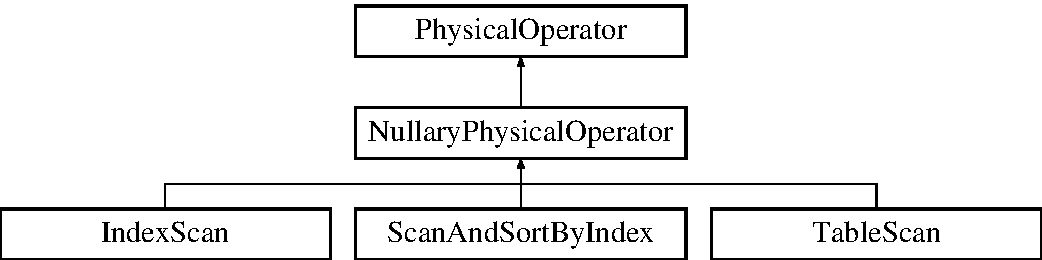
\includegraphics[height=3.000000cm]{class_nullary_physical_operator}
\end{center}
\end{figure}
\subsection*{Public Member Functions}
\begin{DoxyCompactItemize}
\item 
\hypertarget{class_nullary_physical_operator_a053a51bc73b06d883fba982adeeb122c}{virtual void {\bfseries accept} (\hyperlink{class_physical_operator_visitor}{Physical\+Operator\+Visitor} \&v)=0}\label{class_nullary_physical_operator_a053a51bc73b06d883fba982adeeb122c}

\end{DoxyCompactItemize}
\subsection*{Additional Inherited Members}


The documentation for this class was generated from the following file\+:\begin{DoxyCompactItemize}
\item 
C\+:/\+Users/\+Marcel/\+Documents/\+Visual Studio 2012/\+Projects/\+Relational\+Query\+Evaluator/\+Relational\+Query\+Evaluator/Physical\+Operator.\+h\end{DoxyCompactItemize}

\hypertarget{class_number_columns_in_join_visitor}{\section{Number\+Columns\+In\+Join\+Visitor Class Reference}
\label{class_number_columns_in_join_visitor}\index{Number\+Columns\+In\+Join\+Visitor@{Number\+Columns\+In\+Join\+Visitor}}
}
Inheritance diagram for Number\+Columns\+In\+Join\+Visitor\+:\begin{figure}[H]
\begin{center}
\leavevmode
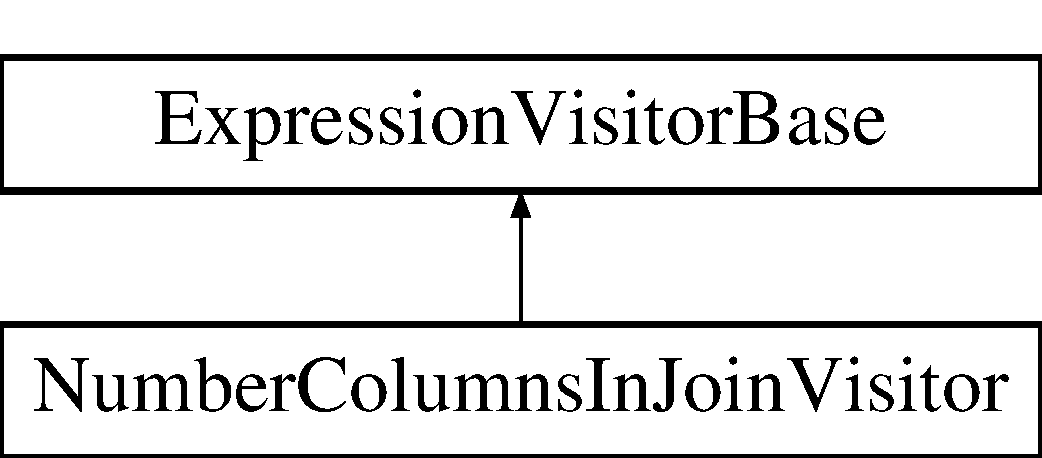
\includegraphics[height=2.000000cm]{class_number_columns_in_join_visitor}
\end{center}
\end{figure}
\subsection*{Public Member Functions}
\begin{DoxyCompactItemize}
\item 
void \hyperlink{class_number_columns_in_join_visitor_ac3b174509ec5ec5310ef73e47aa59694}{visit\+Column} (\hyperlink{class_column}{Column} $\ast$expression)
\item 
void \hyperlink{class_number_columns_in_join_visitor_a857c2d096fe87b1ac98ea50922d1c958}{visit\+Binary\+Expression} (\hyperlink{class_binary_expression}{Binary\+Expression} $\ast$expression)
\end{DoxyCompactItemize}
\subsection*{Public Attributes}
\begin{DoxyCompactItemize}
\item 
\hypertarget{class_number_columns_in_join_visitor_af26374a4ce48016848edd71c935f92a3}{int {\bfseries last\+Numbered\+Column}}\label{class_number_columns_in_join_visitor_af26374a4ce48016848edd71c935f92a3}

\end{DoxyCompactItemize}


\subsection{Member Function Documentation}
\hypertarget{class_number_columns_in_join_visitor_a857c2d096fe87b1ac98ea50922d1c958}{\index{Number\+Columns\+In\+Join\+Visitor@{Number\+Columns\+In\+Join\+Visitor}!visit\+Binary\+Expression@{visit\+Binary\+Expression}}
\index{visit\+Binary\+Expression@{visit\+Binary\+Expression}!Number\+Columns\+In\+Join\+Visitor@{Number\+Columns\+In\+Join\+Visitor}}
\subsubsection[{visit\+Binary\+Expression}]{\setlength{\rightskip}{0pt plus 5cm}void Number\+Columns\+In\+Join\+Visitor\+::visit\+Binary\+Expression (
\begin{DoxyParamCaption}
\item[{{\bf Binary\+Expression} $\ast$}]{expression}
\end{DoxyParamCaption}
)\hspace{0.3cm}{\ttfamily [virtual]}}}\label{class_number_columns_in_join_visitor_a857c2d096fe87b1ac98ea50922d1c958}
Visits \hyperlink{class_binary_expression}{Binary\+Expression} element. 
\begin{DoxyParams}{Parameters}
{\em expression} & visited \hyperlink{class_binary_expression}{Binary\+Expression}. \\
\hline
\end{DoxyParams}


Reimplemented from \hyperlink{class_expression_visitor_base_aebbbbe9a1cecabe4c4804bf1ef82a9f9}{Expression\+Visitor\+Base}.

\hypertarget{class_number_columns_in_join_visitor_ac3b174509ec5ec5310ef73e47aa59694}{\index{Number\+Columns\+In\+Join\+Visitor@{Number\+Columns\+In\+Join\+Visitor}!visit\+Column@{visit\+Column}}
\index{visit\+Column@{visit\+Column}!Number\+Columns\+In\+Join\+Visitor@{Number\+Columns\+In\+Join\+Visitor}}
\subsubsection[{visit\+Column}]{\setlength{\rightskip}{0pt plus 5cm}void Number\+Columns\+In\+Join\+Visitor\+::visit\+Column (
\begin{DoxyParamCaption}
\item[{{\bf Column} $\ast$}]{expression}
\end{DoxyParamCaption}
)\hspace{0.3cm}{\ttfamily [virtual]}}}\label{class_number_columns_in_join_visitor_ac3b174509ec5ec5310ef73e47aa59694}
Visits \hyperlink{class_column}{Column} element. 
\begin{DoxyParams}{Parameters}
{\em expression} & visited \hyperlink{class_column}{Column}. \\
\hline
\end{DoxyParams}


Reimplemented from \hyperlink{class_expression_visitor_base_a1ac638b82248ff9e1582dbf520dc6ae4}{Expression\+Visitor\+Base}.



The documentation for this class was generated from the following files\+:\begin{DoxyCompactItemize}
\item 
C\+:/\+Users/\+Marcel/\+Documents/\+Visual Studio 2012/\+Projects/\+Relational\+Query\+Evaluator/\+Relational\+Query\+Evaluator/Expression\+Visitors.\+h\item 
C\+:/\+Users/\+Marcel/\+Documents/\+Visual Studio 2012/\+Projects/\+Relational\+Query\+Evaluator/\+Relational\+Query\+Evaluator/Expression\+Visitors.\+cpp\end{DoxyCompactItemize}

\hypertarget{class_parser_error_handler}{\section{Parser\+Error\+Handler Class Reference}
\label{class_parser_error_handler}\index{Parser\+Error\+Handler@{Parser\+Error\+Handler}}
}
Inheritance diagram for Parser\+Error\+Handler\+:\begin{figure}[H]
\begin{center}
\leavevmode
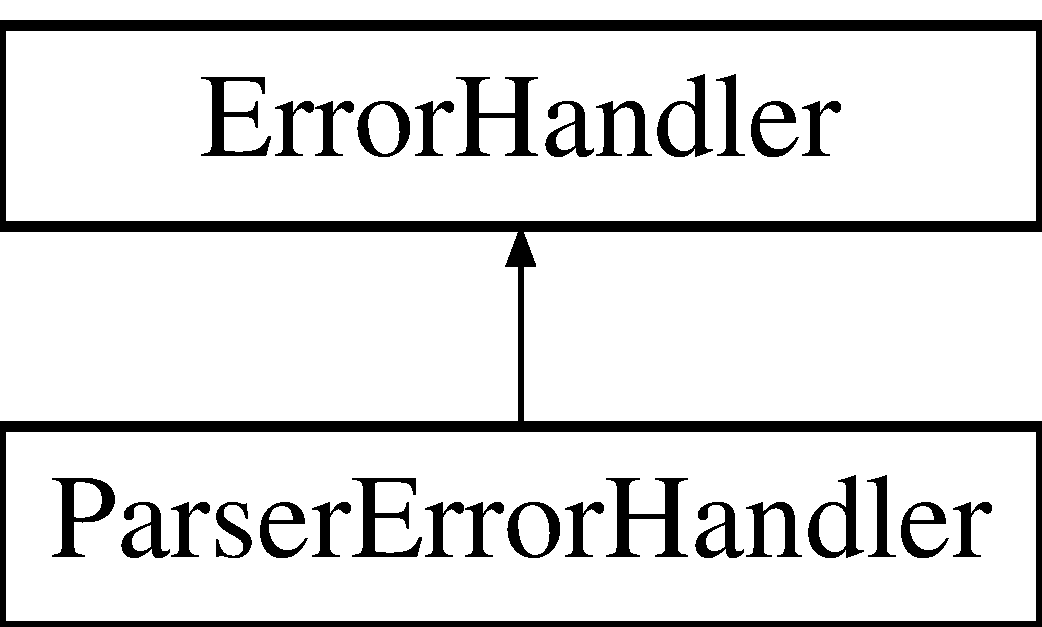
\includegraphics[height=2.000000cm]{class_parser_error_handler}
\end{center}
\end{figure}
\subsection*{Public Member Functions}
\begin{DoxyCompactItemize}
\item 
\hypertarget{class_parser_error_handler_a7e9893b8664f42e38cecb483f0d26791}{void {\bfseries report\+Parse\+Exception} (const S\+A\+X\+Parse\+Exception \&ex)}\label{class_parser_error_handler_a7e9893b8664f42e38cecb483f0d26791}

\item 
\hypertarget{class_parser_error_handler_aa63a6f504a4524985be39e0cdfa4e630}{void {\bfseries warning} (const S\+A\+X\+Parse\+Exception \&ex)}\label{class_parser_error_handler_aa63a6f504a4524985be39e0cdfa4e630}

\item 
\hypertarget{class_parser_error_handler_aa636e61f4f0fb47f38151e09c3711ee7}{void {\bfseries error} (const S\+A\+X\+Parse\+Exception \&ex)}\label{class_parser_error_handler_aa636e61f4f0fb47f38151e09c3711ee7}

\item 
\hypertarget{class_parser_error_handler_a95dede361c7ef584c9a732ca716c61a4}{void {\bfseries fatal\+Error} (const S\+A\+X\+Parse\+Exception \&ex)}\label{class_parser_error_handler_a95dede361c7ef584c9a732ca716c61a4}

\item 
\hypertarget{class_parser_error_handler_afcd94fcf4b801a4767a90b88721b432c}{void {\bfseries reset\+Errors} ()}\label{class_parser_error_handler_afcd94fcf4b801a4767a90b88721b432c}

\item 
\hypertarget{class_parser_error_handler_a1ce19b1e204d760ee30e4f7cd0dfc443}{void {\bfseries set\+Document\+Locator} (const Locator $\ast$const locator)}\label{class_parser_error_handler_a1ce19b1e204d760ee30e4f7cd0dfc443}

\end{DoxyCompactItemize}
\subsection*{Public Attributes}
\begin{DoxyCompactItemize}
\item 
\hypertarget{class_parser_error_handler_a1929eecf90414ca41886580f1d61248f}{int {\bfseries errors}}\label{class_parser_error_handler_a1929eecf90414ca41886580f1d61248f}

\end{DoxyCompactItemize}


The documentation for this class was generated from the following files\+:\begin{DoxyCompactItemize}
\item 
C\+:/\+Users/\+Marcel/\+Documents/\+Visual Studio 2012/\+Projects/\+Relational\+Query\+Evaluator/\+Relational\+Query\+Evaluator/Xml\+Handler.\+h\item 
C\+:/\+Users/\+Marcel/\+Documents/\+Visual Studio 2012/\+Projects/\+Relational\+Query\+Evaluator/\+Relational\+Query\+Evaluator/Xml\+Handler.\+cpp\end{DoxyCompactItemize}

\hypertarget{class_physical_operator}{\section{Physical\+Operator Class Reference}
\label{class_physical_operator}\index{Physical\+Operator@{Physical\+Operator}}
}
Inheritance diagram for Physical\+Operator\+:\begin{figure}[H]
\begin{center}
\leavevmode
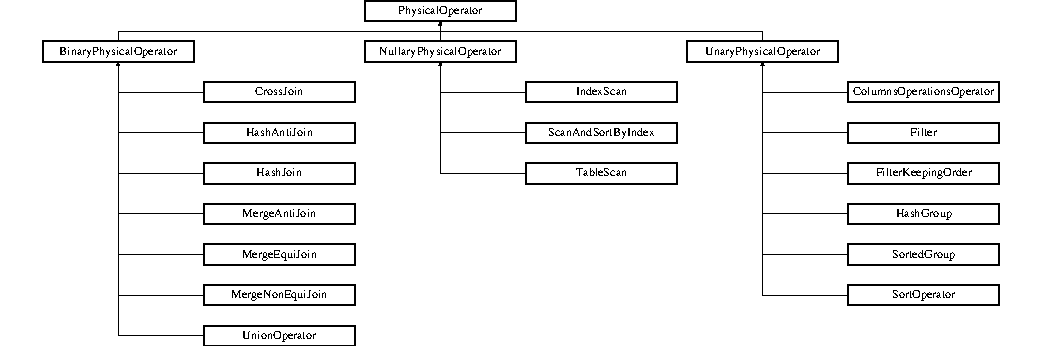
\includegraphics[height=4.640884cm]{class_physical_operator}
\end{center}
\end{figure}
\subsection*{Public Member Functions}
\begin{DoxyCompactItemize}
\item 
\hypertarget{class_physical_operator_aec6926a904c71c0619d6e9e1457252cd}{virtual void {\bfseries accept} (\hyperlink{class_physical_operator_visitor}{Physical\+Operator\+Visitor} \&v)=0}\label{class_physical_operator_aec6926a904c71c0619d6e9e1457252cd}

\end{DoxyCompactItemize}
\subsection*{Public Attributes}
\begin{DoxyCompactItemize}
\item 
\hypertarget{class_physical_operator_a88836a2b6453889b6ad852a2121ca512}{double {\bfseries time\+Complexity}}\label{class_physical_operator_a88836a2b6453889b6ad852a2121ca512}

\item 
\hypertarget{class_physical_operator_a744971579c457601553e8e9a70a5cee1}{double {\bfseries size}}\label{class_physical_operator_a744971579c457601553e8e9a70a5cee1}

\item 
\hypertarget{class_physical_operator_aaf7e49cbadd48e7b0b30e9a84367e5de}{std\+::map$<$ int, \hyperlink{class_column_info}{Column\+Info} $>$ {\bfseries columns}}\label{class_physical_operator_aaf7e49cbadd48e7b0b30e9a84367e5de}

\end{DoxyCompactItemize}


The documentation for this class was generated from the following file\+:\begin{DoxyCompactItemize}
\item 
C\+:/\+Users/\+Marcel/\+Documents/\+Visual Studio 2012/\+Projects/\+Relational\+Query\+Evaluator/\+Relational\+Query\+Evaluator/Physical\+Operator.\+h\end{DoxyCompactItemize}

\hypertarget{class_physical_operator_drawing_visitor}{\section{Physical\+Operator\+Drawing\+Visitor Class Reference}
\label{class_physical_operator_drawing_visitor}\index{Physical\+Operator\+Drawing\+Visitor@{Physical\+Operator\+Drawing\+Visitor}}
}
Inheritance diagram for Physical\+Operator\+Drawing\+Visitor\+:\begin{figure}[H]
\begin{center}
\leavevmode
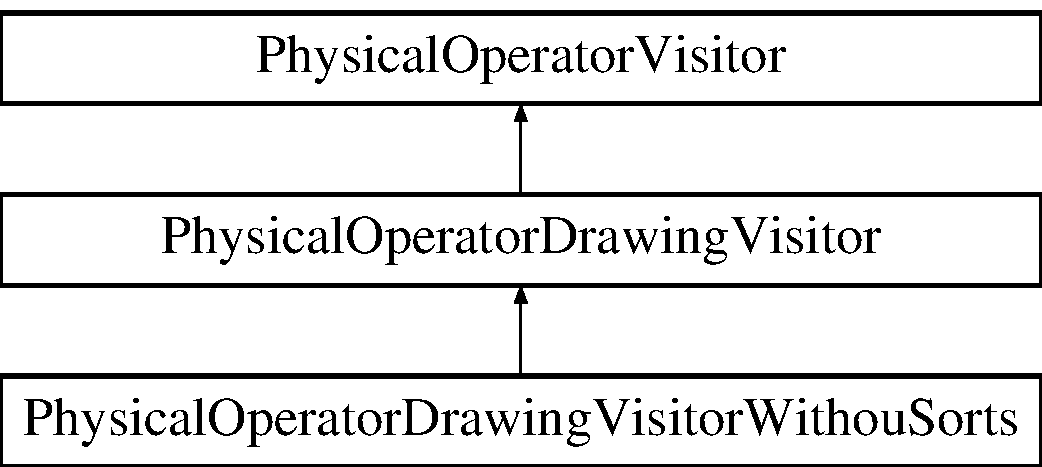
\includegraphics[height=3.000000cm]{class_physical_operator_drawing_visitor}
\end{center}
\end{figure}
\subsection*{Public Member Functions}
\begin{DoxyCompactItemize}
\item 
\hypertarget{class_physical_operator_drawing_visitor_a50acb8aae6d2b5fffff964f7d84b079f}{void {\bfseries generate\+Text} (std\+::string \&label, \hyperlink{class_nullary_physical_operator}{Nullary\+Physical\+Operator} $\ast$node)}\label{class_physical_operator_drawing_visitor_a50acb8aae6d2b5fffff964f7d84b079f}

\item 
\hypertarget{class_physical_operator_drawing_visitor_ab2637eab548a1c1d832a877363ede4a9}{void {\bfseries generate\+Text} (std\+::string \&label, \hyperlink{class_unary_physical_operator}{Unary\+Physical\+Operator} $\ast$node)}\label{class_physical_operator_drawing_visitor_ab2637eab548a1c1d832a877363ede4a9}

\item 
\hypertarget{class_physical_operator_drawing_visitor_a3abc3dcacc46a1004f7a9fb26f56154b}{void {\bfseries generate\+Text} (std\+::string \&label, \hyperlink{class_binary_physical_operator}{Binary\+Physical\+Operator} $\ast$node)}\label{class_physical_operator_drawing_visitor_a3abc3dcacc46a1004f7a9fb26f56154b}

\item 
\hypertarget{class_physical_operator_drawing_visitor_a4729d5a2f38e5318f44149942fb8e3c3}{std\+::string {\bfseries write\+Group\+Parameters} (const std\+::vector$<$ \hyperlink{class_group_column}{Group\+Column} $>$ \&group\+Columns, const std\+::vector$<$ \hyperlink{class_agregate_function}{Agregate\+Function} $>$ \&agregate\+Functions)}\label{class_physical_operator_drawing_visitor_a4729d5a2f38e5318f44149942fb8e3c3}

\item 
\hypertarget{class_physical_operator_drawing_visitor_af5a712a2a8dac447846849d91d20821e}{void {\bfseries visit\+Filter} (\hyperlink{class_filter}{Filter} $\ast$node)}\label{class_physical_operator_drawing_visitor_af5a712a2a8dac447846849d91d20821e}

\item 
\hypertarget{class_physical_operator_drawing_visitor_a0e517a5b635ad9dd2624ca2ac5f623e6}{void {\bfseries visit\+Filter\+Keeping\+Order} (\hyperlink{class_filter_keeping_order}{Filter\+Keeping\+Order} $\ast$node)}\label{class_physical_operator_drawing_visitor_a0e517a5b635ad9dd2624ca2ac5f623e6}

\item 
\hypertarget{class_physical_operator_drawing_visitor_af0aaa68b27e6e562744b0c8211a63b9a}{void {\bfseries visit\+Sort\+Operator} (\hyperlink{class_sort_operator}{Sort\+Operator} $\ast$node)}\label{class_physical_operator_drawing_visitor_af0aaa68b27e6e562744b0c8211a63b9a}

\item 
\hypertarget{class_physical_operator_drawing_visitor_a78f01a744a33b84011ddedca236e95e1}{virtual void {\bfseries visit\+Merge\+Equi\+Join} (\hyperlink{class_merge_equi_join}{Merge\+Equi\+Join} $\ast$node)}\label{class_physical_operator_drawing_visitor_a78f01a744a33b84011ddedca236e95e1}

\item 
\hypertarget{class_physical_operator_drawing_visitor_acdfdd3b9f711abff9fb064495e8512e1}{virtual void {\bfseries visit\+Merge\+Non\+Equi\+Join} (\hyperlink{class_merge_non_equi_join}{Merge\+Non\+Equi\+Join} $\ast$node)}\label{class_physical_operator_drawing_visitor_acdfdd3b9f711abff9fb064495e8512e1}

\item 
\hypertarget{class_physical_operator_drawing_visitor_aaeb9fbec796677a5483384cbddd3f827}{void {\bfseries visit\+Cross\+Join} (\hyperlink{class_cross_join}{Cross\+Join} $\ast$node)}\label{class_physical_operator_drawing_visitor_aaeb9fbec796677a5483384cbddd3f827}

\item 
\hypertarget{class_physical_operator_drawing_visitor_a22032e2685059a3221b85bc990fe684e}{void {\bfseries visit\+Hash\+Join} (\hyperlink{class_hash_join}{Hash\+Join} $\ast$node)}\label{class_physical_operator_drawing_visitor_a22032e2685059a3221b85bc990fe684e}

\item 
\hypertarget{class_physical_operator_drawing_visitor_a1825f8934ad3c2267a40a599b13d2a1a}{void {\bfseries visit\+Hash\+Anti\+Join} (\hyperlink{class_hash_anti_join}{Hash\+Anti\+Join} $\ast$node)}\label{class_physical_operator_drawing_visitor_a1825f8934ad3c2267a40a599b13d2a1a}

\item 
\hypertarget{class_physical_operator_drawing_visitor_ab47caea2d0f82662947a0bf7087e0514}{void {\bfseries visit\+Merge\+Anti\+Join} (\hyperlink{class_merge_anti_join}{Merge\+Anti\+Join} $\ast$node)}\label{class_physical_operator_drawing_visitor_ab47caea2d0f82662947a0bf7087e0514}

\item 
\hypertarget{class_physical_operator_drawing_visitor_aeaa1cd49533ed1bb74921262b918bb06}{void {\bfseries visit\+Union\+Operator} (\hyperlink{class_union_operator}{Union\+Operator} $\ast$node)}\label{class_physical_operator_drawing_visitor_aeaa1cd49533ed1bb74921262b918bb06}

\item 
\hypertarget{class_physical_operator_drawing_visitor_a6841170440f377c240a7c0a7af179a29}{void {\bfseries visit\+Hash\+Group} (\hyperlink{class_hash_group}{Hash\+Group} $\ast$node)}\label{class_physical_operator_drawing_visitor_a6841170440f377c240a7c0a7af179a29}

\item 
\hypertarget{class_physical_operator_drawing_visitor_a1c7736861639025a85d54867d7eeafca}{void {\bfseries visit\+Sorted\+Group} (\hyperlink{class_sorted_group}{Sorted\+Group} $\ast$node)}\label{class_physical_operator_drawing_visitor_a1c7736861639025a85d54867d7eeafca}

\item 
\hypertarget{class_physical_operator_drawing_visitor_ad1fb3f6d50ba14ad674a71e5f6c35d12}{void {\bfseries visit\+Columns\+Operations\+Operator} (\hyperlink{class_columns_operations_operator}{Columns\+Operations\+Operator} $\ast$node)}\label{class_physical_operator_drawing_visitor_ad1fb3f6d50ba14ad674a71e5f6c35d12}

\item 
\hypertarget{class_physical_operator_drawing_visitor_abf3323e213f5c7502e76b0d9afb9fe33}{void {\bfseries visit\+Scan\+And\+Sort\+By\+Index} (\hyperlink{class_scan_and_sort_by_index}{Scan\+And\+Sort\+By\+Index} $\ast$node)}\label{class_physical_operator_drawing_visitor_abf3323e213f5c7502e76b0d9afb9fe33}

\item 
\hypertarget{class_physical_operator_drawing_visitor_a709a44c2c02c9fc42d44fe3822c22f5b}{void {\bfseries visit\+Table\+Scan} (\hyperlink{class_table_scan}{Table\+Scan} $\ast$node)}\label{class_physical_operator_drawing_visitor_a709a44c2c02c9fc42d44fe3822c22f5b}

\item 
\hypertarget{class_physical_operator_drawing_visitor_a3d8f7b6bff44d79fb741b2709587f867}{void {\bfseries visit\+Index\+Scan} (\hyperlink{class_index_scan}{Index\+Scan} $\ast$node)}\label{class_physical_operator_drawing_visitor_a3d8f7b6bff44d79fb741b2709587f867}

\end{DoxyCompactItemize}
\subsection*{Public Attributes}
\begin{DoxyCompactItemize}
\item 
\hypertarget{class_physical_operator_drawing_visitor_a5663f7f6a5c8a6ad25d0c4c8f918123e}{std\+::string {\bfseries result}}\label{class_physical_operator_drawing_visitor_a5663f7f6a5c8a6ad25d0c4c8f918123e}

\item 
\hypertarget{class_physical_operator_drawing_visitor_a75aa4987d070c40a3ec2e4e9c950c9e0}{ulong {\bfseries node\+Counter}}\label{class_physical_operator_drawing_visitor_a75aa4987d070c40a3ec2e4e9c950c9e0}

\end{DoxyCompactItemize}


The documentation for this class was generated from the following files\+:\begin{DoxyCompactItemize}
\item 
C\+:/\+Users/\+Marcel/\+Documents/\+Visual Studio 2012/\+Projects/\+Relational\+Query\+Evaluator/\+Relational\+Query\+Evaluator/Physical\+Operator\+Visitor.\+h\item 
C\+:/\+Users/\+Marcel/\+Documents/\+Visual Studio 2012/\+Projects/\+Relational\+Query\+Evaluator/\+Relational\+Query\+Evaluator/Physical\+Operator\+Visitor.\+cpp\end{DoxyCompactItemize}

\hypertarget{class_physical_operator_drawing_visitor_withou_sorts}{\section{Physical\+Operator\+Drawing\+Visitor\+Withou\+Sorts Class Reference}
\label{class_physical_operator_drawing_visitor_withou_sorts}\index{Physical\+Operator\+Drawing\+Visitor\+Withou\+Sorts@{Physical\+Operator\+Drawing\+Visitor\+Withou\+Sorts}}
}


{\ttfamily \#include $<$Physical\+Operator\+Visitor.\+h$>$}

Inheritance diagram for Physical\+Operator\+Drawing\+Visitor\+Withou\+Sorts\+:\begin{figure}[H]
\begin{center}
\leavevmode
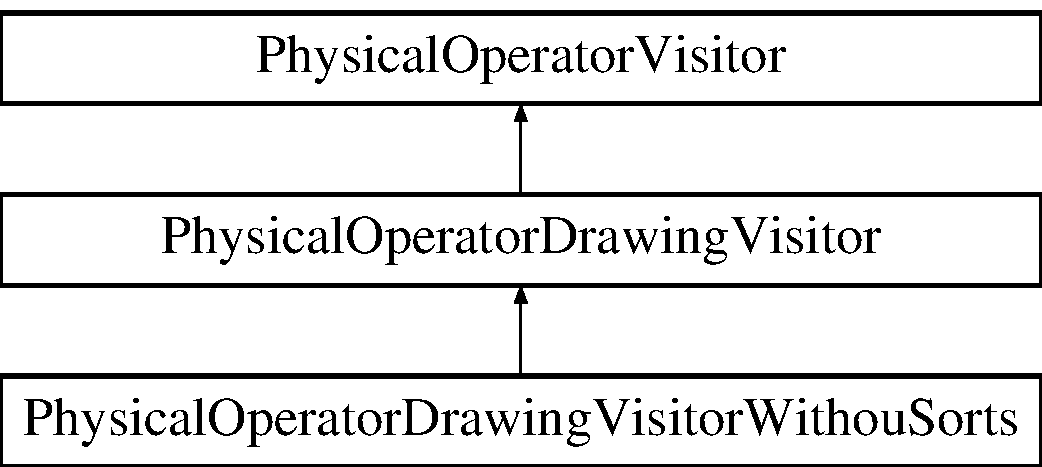
\includegraphics[height=3.000000cm]{class_physical_operator_drawing_visitor_withou_sorts}
\end{center}
\end{figure}
\subsection*{Additional Inherited Members}


\subsection{Detailed Description}
Vsitor generates serialize physical tree to dot code. It is equal to \hyperlink{class_physical_operator_drawing_visitor}{Physical\+Operator\+Drawing\+Visitor} except it doens't write sorts, which output and input are sorted same size. 

The documentation for this class was generated from the following files\+:\begin{DoxyCompactItemize}
\item 
C\+:/\+Users/\+Marcel/\+Documents/\+Visual Studio 2012/\+Projects/\+Relational\+Query\+Evaluator/\+Relational\+Query\+Evaluator/Physical\+Operator\+Visitor.\+h\item 
C\+:/\+Users/\+Marcel/\+Documents/\+Visual Studio 2012/\+Projects/\+Relational\+Query\+Evaluator/\+Relational\+Query\+Evaluator/Physical\+Operator\+Visitor.\+cpp\end{DoxyCompactItemize}

\hypertarget{class_physical_operator_visitor}{\section{Physical\+Operator\+Visitor Class Reference}
\label{class_physical_operator_visitor}\index{Physical\+Operator\+Visitor@{Physical\+Operator\+Visitor}}
}
Inheritance diagram for Physical\+Operator\+Visitor\+:\begin{figure}[H]
\begin{center}
\leavevmode
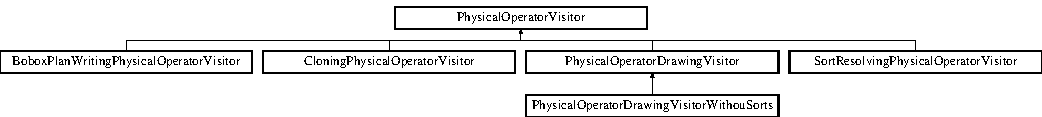
\includegraphics[height=1.561338cm]{class_physical_operator_visitor}
\end{center}
\end{figure}
\subsection*{Public Member Functions}
\begin{DoxyCompactItemize}
\item 
\hypertarget{class_physical_operator_visitor_ade4ed0dbaeb788b5d6dda5aa067ae0b2}{virtual void {\bfseries visit\+Physical\+Operator} (\hyperlink{class_physical_operator}{Physical\+Operator} $\ast$node)}\label{class_physical_operator_visitor_ade4ed0dbaeb788b5d6dda5aa067ae0b2}

\item 
\hypertarget{class_physical_operator_visitor_a03d012d93fa1e96bb95b557bfe0b8d0d}{virtual void {\bfseries visit\+Nullary\+Physical\+Operator} (\hyperlink{class_nullary_physical_operator}{Nullary\+Physical\+Operator} $\ast$node)}\label{class_physical_operator_visitor_a03d012d93fa1e96bb95b557bfe0b8d0d}

\item 
\hypertarget{class_physical_operator_visitor_a9e7270113ed6048b7718dd946ec00ea0}{virtual void {\bfseries visit\+Unary\+Physical\+Operator} (\hyperlink{class_unary_physical_operator}{Unary\+Physical\+Operator} $\ast$node)}\label{class_physical_operator_visitor_a9e7270113ed6048b7718dd946ec00ea0}

\item 
\hypertarget{class_physical_operator_visitor_a19de8665b918063e1be43304aa2286e9}{virtual void {\bfseries visit\+Binary\+Physical\+Operator} (\hyperlink{class_binary_physical_operator}{Binary\+Physical\+Operator} $\ast$node)}\label{class_physical_operator_visitor_a19de8665b918063e1be43304aa2286e9}

\item 
\hypertarget{class_physical_operator_visitor_a30731ff26547314b268e1166f10e57ee}{virtual void {\bfseries visit\+Filter} (\hyperlink{class_filter}{Filter} $\ast$node)}\label{class_physical_operator_visitor_a30731ff26547314b268e1166f10e57ee}

\item 
\hypertarget{class_physical_operator_visitor_a87aa256f7633364ab8fea61a4a20dd19}{virtual void {\bfseries visit\+Filter\+Keeping\+Order} (\hyperlink{class_filter_keeping_order}{Filter\+Keeping\+Order} $\ast$node)}\label{class_physical_operator_visitor_a87aa256f7633364ab8fea61a4a20dd19}

\item 
\hypertarget{class_physical_operator_visitor_ae5f81c64ca3acfa04737fc6655d72767}{virtual void {\bfseries visit\+Sort\+Operator} (\hyperlink{class_sort_operator}{Sort\+Operator} $\ast$node)}\label{class_physical_operator_visitor_ae5f81c64ca3acfa04737fc6655d72767}

\item 
\hypertarget{class_physical_operator_visitor_a4a90fb4cad8fe3ab4877f6ee6f43e1e5}{virtual void {\bfseries visit\+Merge\+Equi\+Join} (\hyperlink{class_merge_equi_join}{Merge\+Equi\+Join} $\ast$node)}\label{class_physical_operator_visitor_a4a90fb4cad8fe3ab4877f6ee6f43e1e5}

\item 
\hypertarget{class_physical_operator_visitor_a9f8bd69369f2fff2bbc74b7aadceaab5}{virtual void {\bfseries visit\+Merge\+Non\+Equi\+Join} (\hyperlink{class_merge_non_equi_join}{Merge\+Non\+Equi\+Join} $\ast$node)}\label{class_physical_operator_visitor_a9f8bd69369f2fff2bbc74b7aadceaab5}

\item 
\hypertarget{class_physical_operator_visitor_a897e543962a692f2725ff7742efae056}{virtual void {\bfseries visit\+Cross\+Join} (\hyperlink{class_cross_join}{Cross\+Join} $\ast$node)}\label{class_physical_operator_visitor_a897e543962a692f2725ff7742efae056}

\item 
\hypertarget{class_physical_operator_visitor_aedb5da87c0637ad8097b7c2eb129129e}{virtual void {\bfseries visit\+Hash\+Join} (\hyperlink{class_hash_join}{Hash\+Join} $\ast$node)}\label{class_physical_operator_visitor_aedb5da87c0637ad8097b7c2eb129129e}

\item 
\hypertarget{class_physical_operator_visitor_af1ce499e2c6db52ed03c3e5f57d144d3}{virtual void {\bfseries visit\+Hash\+Anti\+Join} (\hyperlink{class_hash_anti_join}{Hash\+Anti\+Join} $\ast$node)}\label{class_physical_operator_visitor_af1ce499e2c6db52ed03c3e5f57d144d3}

\item 
\hypertarget{class_physical_operator_visitor_a3d44b3e23abc47c8c0c56938c12ed98a}{virtual void {\bfseries visit\+Merge\+Anti\+Join} (\hyperlink{class_merge_anti_join}{Merge\+Anti\+Join} $\ast$node)}\label{class_physical_operator_visitor_a3d44b3e23abc47c8c0c56938c12ed98a}

\item 
\hypertarget{class_physical_operator_visitor_adbb3e6618904bc7e6d0b6aa3958132e9}{virtual void {\bfseries visit\+Union\+Operator} (\hyperlink{class_union_operator}{Union\+Operator} $\ast$node)}\label{class_physical_operator_visitor_adbb3e6618904bc7e6d0b6aa3958132e9}

\item 
\hypertarget{class_physical_operator_visitor_aa5591d034ce34887c813affc48b7a19c}{virtual void {\bfseries visit\+Hash\+Group} (\hyperlink{class_hash_group}{Hash\+Group} $\ast$node)}\label{class_physical_operator_visitor_aa5591d034ce34887c813affc48b7a19c}

\item 
\hypertarget{class_physical_operator_visitor_a3a3499a62341acf3e49f34ee02a8ed61}{virtual void {\bfseries visit\+Sorted\+Group} (\hyperlink{class_sorted_group}{Sorted\+Group} $\ast$node)}\label{class_physical_operator_visitor_a3a3499a62341acf3e49f34ee02a8ed61}

\item 
\hypertarget{class_physical_operator_visitor_a8c3a41665c8f7ce941532ad9d2052a14}{virtual void {\bfseries visit\+Columns\+Operations\+Operator} (\hyperlink{class_columns_operations_operator}{Columns\+Operations\+Operator} $\ast$node)}\label{class_physical_operator_visitor_a8c3a41665c8f7ce941532ad9d2052a14}

\item 
\hypertarget{class_physical_operator_visitor_ad5551e62c8b00b676577ac6b046be696}{virtual void {\bfseries visit\+Scan\+And\+Sort\+By\+Index} (\hyperlink{class_scan_and_sort_by_index}{Scan\+And\+Sort\+By\+Index} $\ast$node)}\label{class_physical_operator_visitor_ad5551e62c8b00b676577ac6b046be696}

\item 
\hypertarget{class_physical_operator_visitor_a62063b4a4740e730ef7f6728dd926d52}{virtual void {\bfseries visit\+Table\+Scan} (\hyperlink{class_table_scan}{Table\+Scan} $\ast$node)}\label{class_physical_operator_visitor_a62063b4a4740e730ef7f6728dd926d52}

\item 
\hypertarget{class_physical_operator_visitor_ae32578d3229a00be39229a86b575c599}{virtual void {\bfseries visit\+Index\+Scan} (\hyperlink{class_index_scan}{Index\+Scan} $\ast$node)}\label{class_physical_operator_visitor_ae32578d3229a00be39229a86b575c599}

\end{DoxyCompactItemize}


The documentation for this class was generated from the following files\+:\begin{DoxyCompactItemize}
\item 
C\+:/\+Users/\+Marcel/\+Documents/\+Visual Studio 2012/\+Projects/\+Relational\+Query\+Evaluator/\+Relational\+Query\+Evaluator/Physical\+Operator\+Visitor.\+h\item 
C\+:/\+Users/\+Marcel/\+Documents/\+Visual Studio 2012/\+Projects/\+Relational\+Query\+Evaluator/\+Relational\+Query\+Evaluator/Physical\+Operator\+Visitor.\+cpp\end{DoxyCompactItemize}

\hypertarget{class_physical_plan}{\section{Physical\+Plan Class Reference}
\label{class_physical_plan}\index{Physical\+Plan@{Physical\+Plan}}
}
\subsection*{Public Member Functions}
\begin{DoxyCompactItemize}
\item 
\hypertarget{class_physical_plan_a1cf06adf78f2ccb7cbd2d93b119a25f6}{{\bfseries Physical\+Plan} (\hyperlink{class_nullary_physical_operator}{Nullary\+Physical\+Operator} $\ast$op, double number\+Of\+Rows, double time, std\+::vector$<$ \hyperlink{class_column_info}{Column\+Info} $>$ \&cols)}\label{class_physical_plan_a1cf06adf78f2ccb7cbd2d93b119a25f6}

\item 
\hypertarget{class_physical_plan_a7f1bdc130a27a973a12a2da3b66ca43d}{{\bfseries Physical\+Plan} (\hyperlink{class_nullary_physical_operator}{Nullary\+Physical\+Operator} $\ast$op, double number\+Of\+Rows, double time, const std\+::map$<$ int, \hyperlink{class_column_info}{Column\+Info} $>$ \&new\+Columns)}\label{class_physical_plan_a7f1bdc130a27a973a12a2da3b66ca43d}

\item 
\hypertarget{class_physical_plan_a6b8c83da5833167badf7740947297b75}{{\bfseries Physical\+Plan} (\hyperlink{class_unary_physical_operator}{Unary\+Physical\+Operator} $\ast$op, double new\+Size, double time, const std\+::map$<$ int, \hyperlink{class_column_info}{Column\+Info} $>$ \&new\+Columns, const std\+::shared\+\_\+ptr$<$ \hyperlink{class_physical_plan}{Physical\+Plan} $>$ \&old\+Plan)}\label{class_physical_plan_a6b8c83da5833167badf7740947297b75}

\item 
\hypertarget{class_physical_plan_aad6b6a033d32215d38c720904d16a44e}{{\bfseries Physical\+Plan} (\hyperlink{class_binary_physical_operator}{Binary\+Physical\+Operator} $\ast$op, double new\+Size, double time, const std\+::map$<$ int, \hyperlink{class_column_info}{Column\+Info} $>$ \&new\+Columns, const std\+::shared\+\_\+ptr$<$ \hyperlink{class_physical_plan}{Physical\+Plan} $>$ \&old\+Plan1, const std\+::shared\+\_\+ptr$<$ \hyperlink{class_physical_plan}{Physical\+Plan} $>$ \&old\+Plan2)}\label{class_physical_plan_aad6b6a033d32215d38c720904d16a44e}

\end{DoxyCompactItemize}
\subsection*{Static Public Member Functions}
\begin{DoxyCompactItemize}
\item 
\hypertarget{class_physical_plan_a52cbdf31b5d5c9dcdc6730dd1b516e7b}{static bool {\bfseries Comparator} (std\+::shared\+\_\+ptr$<$ \hyperlink{class_physical_plan}{Physical\+Plan} $>$ \&i, std\+::shared\+\_\+ptr$<$ \hyperlink{class_physical_plan}{Physical\+Plan} $>$ \&j)}\label{class_physical_plan_a52cbdf31b5d5c9dcdc6730dd1b516e7b}

\end{DoxyCompactItemize}
\subsection*{Public Attributes}
\begin{DoxyCompactItemize}
\item 
\hypertarget{class_physical_plan_a4d8ba56ef7d228a2a11176da541af5ef}{std\+::vector$<$ \hyperlink{class_index}{Index} $>$ {\bfseries indices}}\label{class_physical_plan_a4d8ba56ef7d228a2a11176da541af5ef}

\item 
\hypertarget{class_physical_plan_a6a49fcbbcb8e22d1f573106de5847c45}{\hyperlink{class_possible_sort_parameters}{Possible\+Sort\+Parameters} {\bfseries sorted\+By}}\label{class_physical_plan_a6a49fcbbcb8e22d1f573106de5847c45}

\item 
\hypertarget{class_physical_plan_a2176d32a64b58406206181395c4127bc}{double {\bfseries time\+Complexity}}\label{class_physical_plan_a2176d32a64b58406206181395c4127bc}

\item 
\hypertarget{class_physical_plan_a97349262f468410057d66f00334003a5}{std\+::shared\+\_\+ptr$<$ \hyperlink{class_physical_operator}{Physical\+Operator} $>$ {\bfseries plan}}\label{class_physical_plan_a97349262f468410057d66f00334003a5}

\end{DoxyCompactItemize}


The documentation for this class was generated from the following files\+:\begin{DoxyCompactItemize}
\item 
C\+:/\+Users/\+Marcel/\+Documents/\+Visual Studio 2012/\+Projects/\+Relational\+Query\+Evaluator/\+Relational\+Query\+Evaluator/Physical\+Operator.\+h\item 
C\+:/\+Users/\+Marcel/\+Documents/\+Visual Studio 2012/\+Projects/\+Relational\+Query\+Evaluator/\+Relational\+Query\+Evaluator/Physical\+Operator.\+cpp\end{DoxyCompactItemize}

\hypertarget{class_possible_sort_parameters}{\section{Possible\+Sort\+Parameters Class Reference}
\label{class_possible_sort_parameters}\index{Possible\+Sort\+Parameters@{Possible\+Sort\+Parameters}}
}
\subsection*{Public Member Functions}
\begin{DoxyCompactItemize}
\item 
\hypertarget{class_possible_sort_parameters_a08aad6763c347ad2a4dc2f20183efc24}{{\bfseries Possible\+Sort\+Parameters} (const std\+::vector$<$ \hyperlink{class_sort_parameters}{Sort\+Parameters} $>$ \&parameters)}\label{class_possible_sort_parameters_a08aad6763c347ad2a4dc2f20183efc24}

\item 
\hypertarget{class_possible_sort_parameters_abf5abacee677c21a76de099cac60aa1a}{{\bfseries Possible\+Sort\+Parameters} (const std\+::vector$<$ \hyperlink{class_sort_parameter}{Sort\+Parameter} $>$ \&parameters)}\label{class_possible_sort_parameters_abf5abacee677c21a76de099cac60aa1a}

\end{DoxyCompactItemize}
\subsection*{Public Attributes}
\begin{DoxyCompactItemize}
\item 
\hypertarget{class_possible_sort_parameters_ac7cd94ff83acacceb9adee62c4228e7f}{std\+::vector$<$ \hyperlink{class_sort_parameters}{Sort\+Parameters} $>$ {\bfseries parameters}}\label{class_possible_sort_parameters_ac7cd94ff83acacceb9adee62c4228e7f}

\end{DoxyCompactItemize}


The documentation for this class was generated from the following files\+:\begin{DoxyCompactItemize}
\item 
C\+:/\+Users/\+Marcel/\+Documents/\+Visual Studio 2012/\+Projects/\+Relational\+Query\+Evaluator/\+Relational\+Query\+Evaluator/Algebra\+Structures.\+h\item 
C\+:/\+Users/\+Marcel/\+Documents/\+Visual Studio 2012/\+Projects/\+Relational\+Query\+Evaluator/\+Relational\+Query\+Evaluator/Algebra\+Structures.\+cpp\end{DoxyCompactItemize}

\hypertarget{class_push_selection_down_visitor}{\section{Push\+Selection\+Down\+Visitor Class Reference}
\label{class_push_selection_down_visitor}\index{Push\+Selection\+Down\+Visitor@{Push\+Selection\+Down\+Visitor}}
}


{\ttfamily \#include $<$Algebra\+Visitors.\+h$>$}

Inheritance diagram for Push\+Selection\+Down\+Visitor\+:\begin{figure}[H]
\begin{center}
\leavevmode
\includegraphics[height=2.000000cm]{class_push_selection_down_visitor}
\end{center}
\end{figure}
\subsection*{Public Member Functions}
\begin{DoxyCompactItemize}
\item 
\hyperlink{class_push_selection_down_visitor_a1be0a28ee1650a54e5c23af1d8effc54}{Push\+Selection\+Down\+Visitor} (\hyperlink{class_selection}{Selection} $\ast$node)
\item 
void \hyperlink{class_push_selection_down_visitor_a343e4e8b9742602455232d5877bf2e15}{push\+Down} ()
\item 
void \hyperlink{class_push_selection_down_visitor_af848a068e14d7c1227fc19411607c463}{visit\+Table} (\hyperlink{class_table}{Table} $\ast$node)
\item 
void \hyperlink{class_push_selection_down_visitor_a15fb2f0fb19d10c40405c4683fd2a2d8}{visit\+Sort} (\hyperlink{class_sort}{Sort} $\ast$node)
\item 
void \hyperlink{class_push_selection_down_visitor_a551561414b97bce56c1bba3829ff9769}{visit\+Group} (\hyperlink{class_group}{Group} $\ast$node)
\item 
void \hyperlink{class_push_selection_down_visitor_a09ade5d0a2d194fee1b5b555d36104a4}{visit\+Column\+Operations} (\hyperlink{class_column_operations}{Column\+Operations} $\ast$node)
\item 
void \hyperlink{class_push_selection_down_visitor_a2534debe115bf3f6648281cc6d0d10ac}{visit\+Selection} (\hyperlink{class_selection}{Selection} $\ast$node)
\item 
void \hyperlink{class_push_selection_down_visitor_a25ff28bccfd9c35119d06117e63465be}{visit\+Join} (\hyperlink{class_join}{Join} $\ast$node)
\item 
void \hyperlink{class_push_selection_down_visitor_a85d6088ea2c478aa85cf62603f30d83a}{visit\+Anti\+Join} (\hyperlink{class_anti_join}{Anti\+Join} $\ast$node)
\item 
void \hyperlink{class_push_selection_down_visitor_a82783e1b22e71264102b53f39d057897}{visit\+Union} (\hyperlink{class_union}{Union} $\ast$node)
\item 
void \hyperlink{class_push_selection_down_visitor_aadf48938c2e165db563095720e10eca6}{visit\+Grouped\+Join} (\hyperlink{class_grouped_join}{Grouped\+Join} $\ast$node)
\end{DoxyCompactItemize}
\subsection*{Additional Inherited Members}


\subsection{Detailed Description}
Visitor takes selection out of the tree and pushes it down the tree as far as possible and inserts it there. 

\subsection{Constructor \& Destructor Documentation}
\hypertarget{class_push_selection_down_visitor_a1be0a28ee1650a54e5c23af1d8effc54}{\index{Push\+Selection\+Down\+Visitor@{Push\+Selection\+Down\+Visitor}!Push\+Selection\+Down\+Visitor@{Push\+Selection\+Down\+Visitor}}
\index{Push\+Selection\+Down\+Visitor@{Push\+Selection\+Down\+Visitor}!Push\+Selection\+Down\+Visitor@{Push\+Selection\+Down\+Visitor}}
\subsubsection[{Push\+Selection\+Down\+Visitor}]{\setlength{\rightskip}{0pt plus 5cm}Push\+Selection\+Down\+Visitor\+::\+Push\+Selection\+Down\+Visitor (
\begin{DoxyParamCaption}
\item[{{\bf Selection} $\ast$}]{node}
\end{DoxyParamCaption}
)}}\label{class_push_selection_down_visitor_a1be0a28ee1650a54e5c23af1d8effc54}
Creates new instance of \hyperlink{class_push_selection_down_visitor}{Push\+Selection\+Down\+Visitor}. 
\begin{DoxyParams}{Parameters}
{\em node} & -\/ node to bu pushed down \\
\hline
\end{DoxyParams}


\subsection{Member Function Documentation}
\hypertarget{class_push_selection_down_visitor_a343e4e8b9742602455232d5877bf2e15}{\index{Push\+Selection\+Down\+Visitor@{Push\+Selection\+Down\+Visitor}!push\+Down@{push\+Down}}
\index{push\+Down@{push\+Down}!Push\+Selection\+Down\+Visitor@{Push\+Selection\+Down\+Visitor}}
\subsubsection[{push\+Down}]{\setlength{\rightskip}{0pt plus 5cm}void Push\+Selection\+Down\+Visitor\+::push\+Down (
\begin{DoxyParamCaption}
{}
\end{DoxyParamCaption}
)}}\label{class_push_selection_down_visitor_a343e4e8b9742602455232d5877bf2e15}
Removes selection and push it down the tree. \hypertarget{class_push_selection_down_visitor_a85d6088ea2c478aa85cf62603f30d83a}{\index{Push\+Selection\+Down\+Visitor@{Push\+Selection\+Down\+Visitor}!visit\+Anti\+Join@{visit\+Anti\+Join}}
\index{visit\+Anti\+Join@{visit\+Anti\+Join}!Push\+Selection\+Down\+Visitor@{Push\+Selection\+Down\+Visitor}}
\subsubsection[{visit\+Anti\+Join}]{\setlength{\rightskip}{0pt plus 5cm}void Push\+Selection\+Down\+Visitor\+::visit\+Anti\+Join (
\begin{DoxyParamCaption}
\item[{{\bf Anti\+Join} $\ast$}]{node}
\end{DoxyParamCaption}
)\hspace{0.3cm}{\ttfamily [virtual]}}}\label{class_push_selection_down_visitor_a85d6088ea2c478aa85cf62603f30d83a}
Visits \hyperlink{class_anti_join}{Anti\+Join} element. 
\begin{DoxyParams}{Parameters}
{\em node} & visited \hyperlink{class_anti_join}{Anti\+Join}. \\
\hline
\end{DoxyParams}


Reimplemented from \hyperlink{class_algebra_visitor_add62415db5f188e572cef1c36faa842e}{Algebra\+Visitor}.

\hypertarget{class_push_selection_down_visitor_a09ade5d0a2d194fee1b5b555d36104a4}{\index{Push\+Selection\+Down\+Visitor@{Push\+Selection\+Down\+Visitor}!visit\+Column\+Operations@{visit\+Column\+Operations}}
\index{visit\+Column\+Operations@{visit\+Column\+Operations}!Push\+Selection\+Down\+Visitor@{Push\+Selection\+Down\+Visitor}}
\subsubsection[{visit\+Column\+Operations}]{\setlength{\rightskip}{0pt plus 5cm}void Push\+Selection\+Down\+Visitor\+::visit\+Column\+Operations (
\begin{DoxyParamCaption}
\item[{{\bf Column\+Operations} $\ast$}]{node}
\end{DoxyParamCaption}
)\hspace{0.3cm}{\ttfamily [virtual]}}}\label{class_push_selection_down_visitor_a09ade5d0a2d194fee1b5b555d36104a4}
Visits \hyperlink{class_column_operations}{Column\+Operations} element. 
\begin{DoxyParams}{Parameters}
{\em node} & visited \hyperlink{class_column_operations}{Column\+Operations}. \\
\hline
\end{DoxyParams}


Reimplemented from \hyperlink{class_algebra_visitor_a1109510d982a8e5b90fc56d443109ef9}{Algebra\+Visitor}.

\hypertarget{class_push_selection_down_visitor_a551561414b97bce56c1bba3829ff9769}{\index{Push\+Selection\+Down\+Visitor@{Push\+Selection\+Down\+Visitor}!visit\+Group@{visit\+Group}}
\index{visit\+Group@{visit\+Group}!Push\+Selection\+Down\+Visitor@{Push\+Selection\+Down\+Visitor}}
\subsubsection[{visit\+Group}]{\setlength{\rightskip}{0pt plus 5cm}void Push\+Selection\+Down\+Visitor\+::visit\+Group (
\begin{DoxyParamCaption}
\item[{{\bf Group} $\ast$}]{node}
\end{DoxyParamCaption}
)\hspace{0.3cm}{\ttfamily [virtual]}}}\label{class_push_selection_down_visitor_a551561414b97bce56c1bba3829ff9769}
Visits \hyperlink{class_group}{Group} element. 
\begin{DoxyParams}{Parameters}
{\em node} & visited \hyperlink{class_group}{Group}. \\
\hline
\end{DoxyParams}


Reimplemented from \hyperlink{class_algebra_visitor_af77bf2aaa949ea27cf992053c43a391b}{Algebra\+Visitor}.

\hypertarget{class_push_selection_down_visitor_aadf48938c2e165db563095720e10eca6}{\index{Push\+Selection\+Down\+Visitor@{Push\+Selection\+Down\+Visitor}!visit\+Grouped\+Join@{visit\+Grouped\+Join}}
\index{visit\+Grouped\+Join@{visit\+Grouped\+Join}!Push\+Selection\+Down\+Visitor@{Push\+Selection\+Down\+Visitor}}
\subsubsection[{visit\+Grouped\+Join}]{\setlength{\rightskip}{0pt plus 5cm}void Push\+Selection\+Down\+Visitor\+::visit\+Grouped\+Join (
\begin{DoxyParamCaption}
\item[{{\bf Grouped\+Join} $\ast$}]{node}
\end{DoxyParamCaption}
)\hspace{0.3cm}{\ttfamily [virtual]}}}\label{class_push_selection_down_visitor_aadf48938c2e165db563095720e10eca6}
Visits \hyperlink{class_grouped_join}{Grouped\+Join} element. 
\begin{DoxyParams}{Parameters}
{\em node} & visited \hyperlink{class_grouped_join}{Grouped\+Join}. \\
\hline
\end{DoxyParams}


Reimplemented from \hyperlink{class_algebra_visitor_ae92c2f0a465dacc4f42a71e879346c94}{Algebra\+Visitor}.

\hypertarget{class_push_selection_down_visitor_a25ff28bccfd9c35119d06117e63465be}{\index{Push\+Selection\+Down\+Visitor@{Push\+Selection\+Down\+Visitor}!visit\+Join@{visit\+Join}}
\index{visit\+Join@{visit\+Join}!Push\+Selection\+Down\+Visitor@{Push\+Selection\+Down\+Visitor}}
\subsubsection[{visit\+Join}]{\setlength{\rightskip}{0pt plus 5cm}void Push\+Selection\+Down\+Visitor\+::visit\+Join (
\begin{DoxyParamCaption}
\item[{{\bf Join} $\ast$}]{node}
\end{DoxyParamCaption}
)\hspace{0.3cm}{\ttfamily [virtual]}}}\label{class_push_selection_down_visitor_a25ff28bccfd9c35119d06117e63465be}
Visits \hyperlink{class_join}{Join} element. 
\begin{DoxyParams}{Parameters}
{\em node} & visited \hyperlink{class_join}{Join}. \\
\hline
\end{DoxyParams}


Reimplemented from \hyperlink{class_algebra_visitor_a841875539a07c979b912ef44455b873c}{Algebra\+Visitor}.

\hypertarget{class_push_selection_down_visitor_a2534debe115bf3f6648281cc6d0d10ac}{\index{Push\+Selection\+Down\+Visitor@{Push\+Selection\+Down\+Visitor}!visit\+Selection@{visit\+Selection}}
\index{visit\+Selection@{visit\+Selection}!Push\+Selection\+Down\+Visitor@{Push\+Selection\+Down\+Visitor}}
\subsubsection[{visit\+Selection}]{\setlength{\rightskip}{0pt plus 5cm}void Push\+Selection\+Down\+Visitor\+::visit\+Selection (
\begin{DoxyParamCaption}
\item[{{\bf Selection} $\ast$}]{node}
\end{DoxyParamCaption}
)\hspace{0.3cm}{\ttfamily [virtual]}}}\label{class_push_selection_down_visitor_a2534debe115bf3f6648281cc6d0d10ac}
Visits \hyperlink{class_selection}{Selection} element. 
\begin{DoxyParams}{Parameters}
{\em node} & visited \hyperlink{class_selection}{Selection}. \\
\hline
\end{DoxyParams}


Reimplemented from \hyperlink{class_algebra_visitor_a7d9b0618ac2fdd036abdab27cbb83d40}{Algebra\+Visitor}.

\hypertarget{class_push_selection_down_visitor_a15fb2f0fb19d10c40405c4683fd2a2d8}{\index{Push\+Selection\+Down\+Visitor@{Push\+Selection\+Down\+Visitor}!visit\+Sort@{visit\+Sort}}
\index{visit\+Sort@{visit\+Sort}!Push\+Selection\+Down\+Visitor@{Push\+Selection\+Down\+Visitor}}
\subsubsection[{visit\+Sort}]{\setlength{\rightskip}{0pt plus 5cm}void Push\+Selection\+Down\+Visitor\+::visit\+Sort (
\begin{DoxyParamCaption}
\item[{{\bf Sort} $\ast$}]{node}
\end{DoxyParamCaption}
)\hspace{0.3cm}{\ttfamily [virtual]}}}\label{class_push_selection_down_visitor_a15fb2f0fb19d10c40405c4683fd2a2d8}
Visits \hyperlink{class_sort}{Sort} element. 
\begin{DoxyParams}{Parameters}
{\em node} & visited \hyperlink{class_sort}{Sort}. \\
\hline
\end{DoxyParams}


Reimplemented from \hyperlink{class_algebra_visitor_ac350bf44664ce021c0cfec18258a14e8}{Algebra\+Visitor}.

\hypertarget{class_push_selection_down_visitor_af848a068e14d7c1227fc19411607c463}{\index{Push\+Selection\+Down\+Visitor@{Push\+Selection\+Down\+Visitor}!visit\+Table@{visit\+Table}}
\index{visit\+Table@{visit\+Table}!Push\+Selection\+Down\+Visitor@{Push\+Selection\+Down\+Visitor}}
\subsubsection[{visit\+Table}]{\setlength{\rightskip}{0pt plus 5cm}void Push\+Selection\+Down\+Visitor\+::visit\+Table (
\begin{DoxyParamCaption}
\item[{{\bf Table} $\ast$}]{node}
\end{DoxyParamCaption}
)\hspace{0.3cm}{\ttfamily [virtual]}}}\label{class_push_selection_down_visitor_af848a068e14d7c1227fc19411607c463}
Visits \hyperlink{class_table}{Table} element. 
\begin{DoxyParams}{Parameters}
{\em node} & visited \hyperlink{class_table}{Table}. \\
\hline
\end{DoxyParams}


Reimplemented from \hyperlink{class_algebra_visitor_ac14f3c3c195373e3bae5d01d04f1ea09}{Algebra\+Visitor}.

\hypertarget{class_push_selection_down_visitor_a82783e1b22e71264102b53f39d057897}{\index{Push\+Selection\+Down\+Visitor@{Push\+Selection\+Down\+Visitor}!visit\+Union@{visit\+Union}}
\index{visit\+Union@{visit\+Union}!Push\+Selection\+Down\+Visitor@{Push\+Selection\+Down\+Visitor}}
\subsubsection[{visit\+Union}]{\setlength{\rightskip}{0pt plus 5cm}void Push\+Selection\+Down\+Visitor\+::visit\+Union (
\begin{DoxyParamCaption}
\item[{{\bf Union} $\ast$}]{node}
\end{DoxyParamCaption}
)\hspace{0.3cm}{\ttfamily [virtual]}}}\label{class_push_selection_down_visitor_a82783e1b22e71264102b53f39d057897}
Visits \hyperlink{class_union}{Union} element. 
\begin{DoxyParams}{Parameters}
{\em node} & visited \hyperlink{class_union}{Union}. \\
\hline
\end{DoxyParams}


Reimplemented from \hyperlink{class_algebra_visitor_a681732083691701f0e9c10980392dd3c}{Algebra\+Visitor}.



The documentation for this class was generated from the following files\+:\begin{DoxyCompactItemize}
\item 
C\+:/\+Users/\+Marcel/\+Documents/\+Visual Studio 2012/\+Projects/\+Relational\+Query\+Evaluator/\+Relational\+Query\+Evaluator/Algebra\+Visitors.\+h\item 
C\+:/\+Users/\+Marcel/\+Documents/\+Visual Studio 2012/\+Projects/\+Relational\+Query\+Evaluator/\+Relational\+Query\+Evaluator/Algebra\+Optimizers.\+cpp\end{DoxyCompactItemize}

\hypertarget{class_rename_columns_visitor}{\section{Rename\+Columns\+Visitor Class Reference}
\label{class_rename_columns_visitor}\index{Rename\+Columns\+Visitor@{Rename\+Columns\+Visitor}}
}
Inheritance diagram for Rename\+Columns\+Visitor\+:\begin{figure}[H]
\begin{center}
\leavevmode
\includegraphics[height=2.000000cm]{class_rename_columns_visitor}
\end{center}
\end{figure}
\subsection*{Public Member Functions}
\begin{DoxyCompactItemize}
\item 
\hypertarget{class_rename_columns_visitor_a119cb79b414164ac4bb2adcfaf6bdcf9}{{\bfseries Rename\+Columns\+Visitor} (std\+::map$<$ int, int $>$ $\ast$pairs)}\label{class_rename_columns_visitor_a119cb79b414164ac4bb2adcfaf6bdcf9}

\item 
\hypertarget{class_rename_columns_visitor_a45835dde3fa3190a803493a0e3f1e75a}{void {\bfseries visit\+Column} (\hyperlink{class_column}{Column} $\ast$expression)}\label{class_rename_columns_visitor_a45835dde3fa3190a803493a0e3f1e75a}

\end{DoxyCompactItemize}
\subsection*{Public Attributes}
\begin{DoxyCompactItemize}
\item 
\hypertarget{class_rename_columns_visitor_a40542b4f59af34a28e298d719ca426c1}{std\+::map$<$ int, int $>$ $\ast$ {\bfseries pairs}}\label{class_rename_columns_visitor_a40542b4f59af34a28e298d719ca426c1}

\end{DoxyCompactItemize}


The documentation for this class was generated from the following file\+:\begin{DoxyCompactItemize}
\item 
C\+:/\+Users/\+Marcel/\+Documents/\+Visual Studio 2012/\+Projects/\+Relational\+Query\+Evaluator/\+Relational\+Query\+Evaluator/Expression\+Visitors.\+h\end{DoxyCompactItemize}

\hypertarget{class_renaming_join_condition_expression_visitor}{\section{Renaming\+Join\+Condition\+Expression\+Visitor Class Reference}
\label{class_renaming_join_condition_expression_visitor}\index{Renaming\+Join\+Condition\+Expression\+Visitor@{Renaming\+Join\+Condition\+Expression\+Visitor}}
}
Inheritance diagram for Renaming\+Join\+Condition\+Expression\+Visitor\+:\begin{figure}[H]
\begin{center}
\leavevmode
\includegraphics[height=2.000000cm]{class_renaming_join_condition_expression_visitor}
\end{center}
\end{figure}
\subsection*{Public Member Functions}
\begin{DoxyCompactItemize}
\item 
\hypertarget{class_renaming_join_condition_expression_visitor_a2b0669f3664fd3b9170e431bfcde9851}{{\bfseries Renaming\+Join\+Condition\+Expression\+Visitor} (ulong i, std\+::vector$<$ \hyperlink{class_join_column_info}{Join\+Column\+Info} $>$ $\ast$input\+Columns)}\label{class_renaming_join_condition_expression_visitor_a2b0669f3664fd3b9170e431bfcde9851}

\item 
\hypertarget{class_renaming_join_condition_expression_visitor_aa55184f591960115d4e11eff4be0d3d5}{void {\bfseries visit\+Column} (\hyperlink{class_column}{Column} $\ast$expression)}\label{class_renaming_join_condition_expression_visitor_aa55184f591960115d4e11eff4be0d3d5}

\end{DoxyCompactItemize}
\subsection*{Public Attributes}
\begin{DoxyCompactItemize}
\item 
\hypertarget{class_renaming_join_condition_expression_visitor_aa9eacf839bdb9a30653d5cae0448532b}{ulong {\bfseries n}}\label{class_renaming_join_condition_expression_visitor_aa9eacf839bdb9a30653d5cae0448532b}

\item 
\hypertarget{class_renaming_join_condition_expression_visitor_a8b8dceeedbf7c4d3aac3761ce3a4c302}{std\+::vector$<$ \hyperlink{class_join_column_info}{Join\+Column\+Info} $>$ $\ast$ {\bfseries input\+Columns}}\label{class_renaming_join_condition_expression_visitor_a8b8dceeedbf7c4d3aac3761ce3a4c302}

\end{DoxyCompactItemize}


The documentation for this class was generated from the following file\+:\begin{DoxyCompactItemize}
\item 
C\+:/\+Users/\+Marcel/\+Documents/\+Visual Studio 2012/\+Projects/\+Relational\+Query\+Evaluator/\+Relational\+Query\+Evaluator/Expression\+Visitors.\+h\end{DoxyCompactItemize}

\hypertarget{class_scan_and_sort_by_index}{\section{Scan\+And\+Sort\+By\+Index Class Reference}
\label{class_scan_and_sort_by_index}\index{Scan\+And\+Sort\+By\+Index@{Scan\+And\+Sort\+By\+Index}}
}
Inheritance diagram for Scan\+And\+Sort\+By\+Index\+:\begin{figure}[H]
\begin{center}
\leavevmode
\includegraphics[height=3.000000cm]{class_scan_and_sort_by_index}
\end{center}
\end{figure}
\subsection*{Public Member Functions}
\begin{DoxyCompactItemize}
\item 
\hypertarget{class_scan_and_sort_by_index_a8304f98fd2eea171365ad996666fdd01}{{\bfseries Scan\+And\+Sort\+By\+Index} (const std\+::string \&name, const \hyperlink{class_index}{Index} \&index)}\label{class_scan_and_sort_by_index_a8304f98fd2eea171365ad996666fdd01}

\item 
\hypertarget{class_scan_and_sort_by_index_a9e0d99d88104c8215bacb470e298b363}{void {\bfseries accept} (\hyperlink{class_physical_operator_visitor}{Physical\+Operator\+Visitor} \&v)}\label{class_scan_and_sort_by_index_a9e0d99d88104c8215bacb470e298b363}

\end{DoxyCompactItemize}
\subsection*{Public Attributes}
\begin{DoxyCompactItemize}
\item 
\hypertarget{class_scan_and_sort_by_index_a04ad43495fcb141d4e7c51d9907f3a42}{std\+::string {\bfseries table\+Name}}\label{class_scan_and_sort_by_index_a04ad43495fcb141d4e7c51d9907f3a42}

\item 
\hypertarget{class_scan_and_sort_by_index_a132a795383838f5cc3e6c17288509e15}{\hyperlink{class_index}{Index} {\bfseries index}}\label{class_scan_and_sort_by_index_a132a795383838f5cc3e6c17288509e15}

\end{DoxyCompactItemize}


The documentation for this class was generated from the following files\+:\begin{DoxyCompactItemize}
\item 
C\+:/\+Users/\+Marcel/\+Documents/\+Visual Studio 2012/\+Projects/\+Relational\+Query\+Evaluator/\+Relational\+Query\+Evaluator/Physical\+Operator.\+h\item 
C\+:/\+Users/\+Marcel/\+Documents/\+Visual Studio 2012/\+Projects/\+Relational\+Query\+Evaluator/\+Relational\+Query\+Evaluator/Physical\+Operator.\+cpp\end{DoxyCompactItemize}

\hypertarget{class_selection}{\section{Selection Class Reference}
\label{class_selection}\index{Selection@{Selection}}
}


{\ttfamily \#include $<$Algebra.\+h$>$}

Inheritance diagram for Selection\+:\begin{figure}[H]
\begin{center}
\leavevmode
\includegraphics[height=3.000000cm]{class_selection}
\end{center}
\end{figure}
\subsection*{Public Member Functions}
\begin{DoxyCompactItemize}
\item 
\hyperlink{class_selection_a53d1bd270d6d257d34d5bc8d50028049}{Selection} ()
\item 
\hyperlink{class_selection_a83b3073a2d490708256e3dc725560836}{Selection} (D\+O\+M\+Element $\ast$element)
\item 
\hyperlink{class_selection_a086ad5ebceb2f48c7b66c150c4f1d92c}{Selection} (std\+::shared\+\_\+ptr$<$ \hyperlink{class_expression}{Expression} $>$ \&cond)
\item 
void \hyperlink{class_selection_afe7f64aed777d583797f1c9c13b378ac}{accept} (\hyperlink{class_algebra_visitor}{Algebra\+Visitor} \&v)
\end{DoxyCompactItemize}
\subsection*{Public Attributes}
\begin{DoxyCompactItemize}
\item 
std\+::shared\+\_\+ptr$<$ \hyperlink{class_expression}{Expression} $>$ \hyperlink{class_selection_a2356634cb924e5b5814c4d2bfee51d65}{condition}
\end{DoxyCompactItemize}


\subsection{Detailed Description}
Represents algebraic operation selection. It filters input rows and copies to output only rows satisfying given condition. 

\subsection{Constructor \& Destructor Documentation}
\hypertarget{class_selection_a53d1bd270d6d257d34d5bc8d50028049}{\index{Selection@{Selection}!Selection@{Selection}}
\index{Selection@{Selection}!Selection@{Selection}}
\subsubsection[{Selection}]{\setlength{\rightskip}{0pt plus 5cm}Selection\+::\+Selection (
\begin{DoxyParamCaption}
{}
\end{DoxyParamCaption}
)}}\label{class_selection_a53d1bd270d6d257d34d5bc8d50028049}
Create the instance of \hyperlink{class_selection}{Selection}. \hypertarget{class_selection_a83b3073a2d490708256e3dc725560836}{\index{Selection@{Selection}!Selection@{Selection}}
\index{Selection@{Selection}!Selection@{Selection}}
\subsubsection[{Selection}]{\setlength{\rightskip}{0pt plus 5cm}Selection\+::\+Selection (
\begin{DoxyParamCaption}
\item[{D\+O\+M\+Element $\ast$}]{element}
\end{DoxyParamCaption}
)}}\label{class_selection_a83b3073a2d490708256e3dc725560836}
Create the instance of \hyperlink{class_selection}{Selection}. 
\begin{DoxyParams}{Parameters}
{\em element} & representing input node. \\
\hline
\end{DoxyParams}
\hypertarget{class_selection_a086ad5ebceb2f48c7b66c150c4f1d92c}{\index{Selection@{Selection}!Selection@{Selection}}
\index{Selection@{Selection}!Selection@{Selection}}
\subsubsection[{Selection}]{\setlength{\rightskip}{0pt plus 5cm}Selection\+::\+Selection (
\begin{DoxyParamCaption}
\item[{std\+::shared\+\_\+ptr$<$ {\bf Expression} $>$ \&}]{cond}
\end{DoxyParamCaption}
)}}\label{class_selection_a086ad5ebceb2f48c7b66c150c4f1d92c}
Create the instance of \hyperlink{class_selection}{Selection}. 
\begin{DoxyParams}{Parameters}
{\em cond} & \hyperlink{class_expression}{Expression} -\/ filter condition \\
\hline
\end{DoxyParams}


\subsection{Member Function Documentation}
\hypertarget{class_selection_afe7f64aed777d583797f1c9c13b378ac}{\index{Selection@{Selection}!accept@{accept}}
\index{accept@{accept}!Selection@{Selection}}
\subsubsection[{accept}]{\setlength{\rightskip}{0pt plus 5cm}void Selection\+::accept (
\begin{DoxyParamCaption}
\item[{{\bf Algebra\+Visitor} \&}]{v}
\end{DoxyParamCaption}
)\hspace{0.3cm}{\ttfamily [virtual]}}}\label{class_selection_afe7f64aed777d583797f1c9c13b378ac}
Method for calling visit\mbox{[}node\mbox{]} on given \hyperlink{class_algebra_visitor}{Algebra\+Visitor} 
\begin{DoxyParams}{Parameters}
{\em v} & \hyperlink{class_algebra_visitor}{Algebra\+Visitor}, on which to call function \\
\hline
\end{DoxyParams}


Implements \hyperlink{class_unary_algebra_node_base_a33355111a226cb460c9a13efaf922e32}{Unary\+Algebra\+Node\+Base}.



\subsection{Member Data Documentation}
\hypertarget{class_selection_a2356634cb924e5b5814c4d2bfee51d65}{\index{Selection@{Selection}!condition@{condition}}
\index{condition@{condition}!Selection@{Selection}}
\subsubsection[{condition}]{\setlength{\rightskip}{0pt plus 5cm}std\+::shared\+\_\+ptr$<${\bf Expression}$>$ Selection\+::condition}}\label{class_selection_a2356634cb924e5b5814c4d2bfee51d65}
Condition for filtering given input. 

The documentation for this class was generated from the following files\+:\begin{DoxyCompactItemize}
\item 
C\+:/\+Users/\+Marcel/\+Documents/\+Visual Studio 2012/\+Projects/\+Relational\+Query\+Evaluator/\+Relational\+Query\+Evaluator/Algebra.\+h\item 
C\+:/\+Users/\+Marcel/\+Documents/\+Visual Studio 2012/\+Projects/\+Relational\+Query\+Evaluator/\+Relational\+Query\+Evaluator/Algebra.\+cpp\end{DoxyCompactItemize}

\hypertarget{class_selection_colecting_visitor}{\section{Selection\+Colecting\+Visitor Class Reference}
\label{class_selection_colecting_visitor}\index{Selection\+Colecting\+Visitor@{Selection\+Colecting\+Visitor}}
}
Inheritance diagram for Selection\+Colecting\+Visitor\+:\begin{figure}[H]
\begin{center}
\leavevmode
\includegraphics[height=2.000000cm]{class_selection_colecting_visitor}
\end{center}
\end{figure}
\subsection*{Public Member Functions}
\begin{DoxyCompactItemize}
\item 
\hypertarget{class_selection_colecting_visitor_a29c5a9ecf7dbfdc4b563b94385c61de3}{void {\bfseries visit\+Selection} (\hyperlink{class_selection}{Selection} $\ast$node)}\label{class_selection_colecting_visitor_a29c5a9ecf7dbfdc4b563b94385c61de3}

\end{DoxyCompactItemize}
\subsection*{Public Attributes}
\begin{DoxyCompactItemize}
\item 
\hypertarget{class_selection_colecting_visitor_a6323b360276b0ff23f5dcaa19b2317eb}{std\+::vector$<$ \hyperlink{class_selection}{Selection} $\ast$ $>$ {\bfseries selections}}\label{class_selection_colecting_visitor_a6323b360276b0ff23f5dcaa19b2317eb}

\end{DoxyCompactItemize}
\subsection*{Additional Inherited Members}


The documentation for this class was generated from the following files\+:\begin{DoxyCompactItemize}
\item 
C\+:/\+Users/\+Marcel/\+Documents/\+Visual Studio 2012/\+Projects/\+Relational\+Query\+Evaluator/\+Relational\+Query\+Evaluator/Algebra\+Visitors.\+h\item 
C\+:/\+Users/\+Marcel/\+Documents/\+Visual Studio 2012/\+Projects/\+Relational\+Query\+Evaluator/\+Relational\+Query\+Evaluator/Algebra\+Optimizers.\+cpp\end{DoxyCompactItemize}

\hypertarget{class_selection_fusing_visitor}{\section{Selection\+Fusing\+Visitor Class Reference}
\label{class_selection_fusing_visitor}\index{Selection\+Fusing\+Visitor@{Selection\+Fusing\+Visitor}}
}


{\ttfamily \#include $<$Algebra\+Visitors.\+h$>$}

Inheritance diagram for Selection\+Fusing\+Visitor\+:\begin{figure}[H]
\begin{center}
\leavevmode
\includegraphics[height=2.000000cm]{class_selection_fusing_visitor}
\end{center}
\end{figure}
\subsection*{Public Member Functions}
\begin{DoxyCompactItemize}
\item 
void \hyperlink{class_selection_fusing_visitor_af7999d106685c9938c907c6984ba4f2d}{visit\+Selection} (\hyperlink{class_selection}{Selection} $\ast$node)
\end{DoxyCompactItemize}
\subsection*{Additional Inherited Members}


\subsection{Detailed Description}
Merges neighbouring selections into one selection and insert it into tree instred of original chain of selections. 

\subsection{Member Function Documentation}
\hypertarget{class_selection_fusing_visitor_af7999d106685c9938c907c6984ba4f2d}{\index{Selection\+Fusing\+Visitor@{Selection\+Fusing\+Visitor}!visit\+Selection@{visit\+Selection}}
\index{visit\+Selection@{visit\+Selection}!Selection\+Fusing\+Visitor@{Selection\+Fusing\+Visitor}}
\subsubsection[{visit\+Selection}]{\setlength{\rightskip}{0pt plus 5cm}void Selection\+Fusing\+Visitor\+::visit\+Selection (
\begin{DoxyParamCaption}
\item[{{\bf Selection} $\ast$}]{node}
\end{DoxyParamCaption}
)\hspace{0.3cm}{\ttfamily [virtual]}}}\label{class_selection_fusing_visitor_af7999d106685c9938c907c6984ba4f2d}
Visits \hyperlink{class_selection}{Selection} element. 
\begin{DoxyParams}{Parameters}
{\em node} & visited \hyperlink{class_selection}{Selection}. \\
\hline
\end{DoxyParams}


Reimplemented from \hyperlink{class_algebra_visitor_a7d9b0618ac2fdd036abdab27cbb83d40}{Algebra\+Visitor}.



The documentation for this class was generated from the following files\+:\begin{DoxyCompactItemize}
\item 
C\+:/\+Users/\+Marcel/\+Documents/\+Visual Studio 2012/\+Projects/\+Relational\+Query\+Evaluator/\+Relational\+Query\+Evaluator/Algebra\+Visitors.\+h\item 
C\+:/\+Users/\+Marcel/\+Documents/\+Visual Studio 2012/\+Projects/\+Relational\+Query\+Evaluator/\+Relational\+Query\+Evaluator/Algebra\+Optimizers.\+cpp\end{DoxyCompactItemize}

\hypertarget{class_selection_spiting_visitor}{\section{Selection\+Spiting\+Visitor Class Reference}
\label{class_selection_spiting_visitor}\index{Selection\+Spiting\+Visitor@{Selection\+Spiting\+Visitor}}
}


{\ttfamily \#include $<$Algebra\+Visitors.\+h$>$}

Inheritance diagram for Selection\+Spiting\+Visitor\+:\begin{figure}[H]
\begin{center}
\leavevmode
\includegraphics[height=2.000000cm]{class_selection_spiting_visitor}
\end{center}
\end{figure}
\subsection*{Public Member Functions}
\begin{DoxyCompactItemize}
\item 
void \hyperlink{class_selection_spiting_visitor_ac494bc17989d4fe23736f6ce55972aba}{visit\+Selection} (\hyperlink{class_selection}{Selection} $\ast$node)
\end{DoxyCompactItemize}
\subsection*{Additional Inherited Members}


\subsection{Detailed Description}
Splits selections into partial condition and insert them into tree at place where the original selection was. 

\subsection{Member Function Documentation}
\hypertarget{class_selection_spiting_visitor_ac494bc17989d4fe23736f6ce55972aba}{\index{Selection\+Spiting\+Visitor@{Selection\+Spiting\+Visitor}!visit\+Selection@{visit\+Selection}}
\index{visit\+Selection@{visit\+Selection}!Selection\+Spiting\+Visitor@{Selection\+Spiting\+Visitor}}
\subsubsection[{visit\+Selection}]{\setlength{\rightskip}{0pt plus 5cm}void Selection\+Spiting\+Visitor\+::visit\+Selection (
\begin{DoxyParamCaption}
\item[{{\bf Selection} $\ast$}]{node}
\end{DoxyParamCaption}
)\hspace{0.3cm}{\ttfamily [virtual]}}}\label{class_selection_spiting_visitor_ac494bc17989d4fe23736f6ce55972aba}
Visits \hyperlink{class_selection}{Selection} element. 
\begin{DoxyParams}{Parameters}
{\em node} & visited \hyperlink{class_selection}{Selection}. \\
\hline
\end{DoxyParams}


Reimplemented from \hyperlink{class_algebra_visitor_a7d9b0618ac2fdd036abdab27cbb83d40}{Algebra\+Visitor}.



The documentation for this class was generated from the following files\+:\begin{DoxyCompactItemize}
\item 
C\+:/\+Users/\+Marcel/\+Documents/\+Visual Studio 2012/\+Projects/\+Relational\+Query\+Evaluator/\+Relational\+Query\+Evaluator/Algebra\+Visitors.\+h\item 
C\+:/\+Users/\+Marcel/\+Documents/\+Visual Studio 2012/\+Projects/\+Relational\+Query\+Evaluator/\+Relational\+Query\+Evaluator/Algebra\+Optimizers.\+cpp\end{DoxyCompactItemize}

\hypertarget{class_semantic_checker}{\section{Semantic\+Checker Class Reference}
\label{class_semantic_checker}\index{Semantic\+Checker@{Semantic\+Checker}}
}


{\ttfamily \#include $<$Algebra\+Visitors.\+h$>$}

Inheritance diagram for Semantic\+Checker\+:\begin{figure}[H]
\begin{center}
\leavevmode
\includegraphics[height=2.000000cm]{class_semantic_checker}
\end{center}
\end{figure}
\subsection*{Public Member Functions}
\begin{DoxyCompactItemize}
\item 
\hyperlink{class_semantic_checker_a35a20bf073bd1fdf1de937db47b9f4c0}{Semantic\+Checker} ()
\item 
int \hyperlink{class_semantic_checker_a7bfc82245e0af345db051ab8faea502e}{next\+Id} ()
\item 
{\footnotesize template$<$typename T $>$ }\\void \hyperlink{class_semantic_checker_a31d420801c78aaf317a4b0094f9da3df}{check\+Join\+Out\+Put\+Parameters} (std\+::map$<$ std\+::string, \hyperlink{class_column_info}{Column\+Info} $>$ \&output\+Columns0, std\+::map$<$ std\+::string, \hyperlink{class_column_info}{Column\+Info} $>$ \&output\+Columns1, T $\ast$node)
\item 
void \hyperlink{class_semantic_checker_a915d3f58ab60a0e6ba6f248e3c81f0c5}{visit\+Table} (\hyperlink{class_table}{Table} $\ast$node)
\item 
void \hyperlink{class_semantic_checker_ae7cbd8a1c92f544a282de4b741d1e19e}{visit\+Sort} (\hyperlink{class_sort}{Sort} $\ast$node)
\item 
void \hyperlink{class_semantic_checker_a8dfc703b185f05a0f57749e1eb3c0a56}{visit\+Group} (\hyperlink{class_group}{Group} $\ast$node)
\item 
void \hyperlink{class_semantic_checker_a5bd2ca32010822a95a6ef0a78190fc91}{visit\+Column\+Operations} (\hyperlink{class_column_operations}{Column\+Operations} $\ast$node)
\item 
void \hyperlink{class_semantic_checker_ac2825bf63bbda696b461166f915bacfe}{visit\+Selection} (\hyperlink{class_selection}{Selection} $\ast$node)
\item 
void \hyperlink{class_semantic_checker_a047de398ed6fab98a4ec6c1db533a66e}{visit\+Join} (\hyperlink{class_join}{Join} $\ast$node)
\item 
void \hyperlink{class_semantic_checker_aed141e3f22e681c74355fb3b84deb2d4}{visit\+Anti\+Join} (\hyperlink{class_anti_join}{Anti\+Join} $\ast$node)
\item 
void \hyperlink{class_semantic_checker_a120a86891155bd0296b9f3e878462bc6}{visit\+Union} (\hyperlink{class_union}{Union} $\ast$node)
\item 
void \hyperlink{class_semantic_checker_a44c4c5cf8cde9785a2a11f446d8fb90a}{visit\+Grouped\+Join} (\hyperlink{class_grouped_join}{Grouped\+Join} $\ast$node)
\end{DoxyCompactItemize}
\subsection*{Public Attributes}
\begin{DoxyCompactItemize}
\item 
bool \hyperlink{class_semantic_checker_a3683f9e8bd069bf8b76c42ea6ff11b96}{contains\+Errors}
\end{DoxyCompactItemize}
\subsection*{Additional Inherited Members}


\subsection{Detailed Description}
This visitor is checking\+:
\begin{DoxyItemize}
\item if all the requested columns exists
\item if the columns are not declared multiple times. Then if error is reported, compilation cannot continue. It also gives columns unique identifier, so other vistors don't have to work with string names. 
\end{DoxyItemize}

\subsection{Constructor \& Destructor Documentation}
\hypertarget{class_semantic_checker_a35a20bf073bd1fdf1de937db47b9f4c0}{\index{Semantic\+Checker@{Semantic\+Checker}!Semantic\+Checker@{Semantic\+Checker}}
\index{Semantic\+Checker@{Semantic\+Checker}!Semantic\+Checker@{Semantic\+Checker}}
\subsubsection[{Semantic\+Checker}]{\setlength{\rightskip}{0pt plus 5cm}Semantic\+Checker\+::\+Semantic\+Checker (
\begin{DoxyParamCaption}
{}
\end{DoxyParamCaption}
)}}\label{class_semantic_checker_a35a20bf073bd1fdf1de937db47b9f4c0}
Creates new instance of \hyperlink{class_semantic_checker}{Semantic\+Checker}. 

\subsection{Member Function Documentation}
\hypertarget{class_semantic_checker_a31d420801c78aaf317a4b0094f9da3df}{\index{Semantic\+Checker@{Semantic\+Checker}!check\+Join\+Out\+Put\+Parameters@{check\+Join\+Out\+Put\+Parameters}}
\index{check\+Join\+Out\+Put\+Parameters@{check\+Join\+Out\+Put\+Parameters}!Semantic\+Checker@{Semantic\+Checker}}
\subsubsection[{check\+Join\+Out\+Put\+Parameters}]{\setlength{\rightskip}{0pt plus 5cm}template$<$typename T $>$ void Semantic\+Checker\+::check\+Join\+Out\+Put\+Parameters (
\begin{DoxyParamCaption}
\item[{std\+::map$<$ std\+::string, {\bf Column\+Info} $>$ \&}]{output\+Columns0, }
\item[{std\+::map$<$ std\+::string, {\bf Column\+Info} $>$ \&}]{output\+Columns1, }
\item[{T $\ast$}]{node}
\end{DoxyParamCaption}
)\hspace{0.3cm}{\ttfamily [inline]}}}\label{class_semantic_checker_a31d420801c78aaf317a4b0094f9da3df}
Checks join condition and output columns and reports semantic errors. 
\begin{DoxyParams}{Parameters}
{\em output\+Columns0} & -\/ output columns from first join input \\
\hline
{\em output\+Columns1} & -\/ output columns from second join input \\
\hline
{\em node} & -\/ node join or antijoin node \\
\hline
\end{DoxyParams}
\hypertarget{class_semantic_checker_a7bfc82245e0af345db051ab8faea502e}{\index{Semantic\+Checker@{Semantic\+Checker}!next\+Id@{next\+Id}}
\index{next\+Id@{next\+Id}!Semantic\+Checker@{Semantic\+Checker}}
\subsubsection[{next\+Id}]{\setlength{\rightskip}{0pt plus 5cm}int Semantic\+Checker\+::next\+Id (
\begin{DoxyParamCaption}
{}
\end{DoxyParamCaption}
)}}\label{class_semantic_checker_a7bfc82245e0af345db051ab8faea502e}
Generates new unique column identifier. \begin{DoxyReturn}{Returns}
new unique identifier 
\end{DoxyReturn}
\hypertarget{class_semantic_checker_aed141e3f22e681c74355fb3b84deb2d4}{\index{Semantic\+Checker@{Semantic\+Checker}!visit\+Anti\+Join@{visit\+Anti\+Join}}
\index{visit\+Anti\+Join@{visit\+Anti\+Join}!Semantic\+Checker@{Semantic\+Checker}}
\subsubsection[{visit\+Anti\+Join}]{\setlength{\rightskip}{0pt plus 5cm}void Semantic\+Checker\+::visit\+Anti\+Join (
\begin{DoxyParamCaption}
\item[{{\bf Anti\+Join} $\ast$}]{node}
\end{DoxyParamCaption}
)\hspace{0.3cm}{\ttfamily [virtual]}}}\label{class_semantic_checker_aed141e3f22e681c74355fb3b84deb2d4}
Visits \hyperlink{class_anti_join}{Anti\+Join} element. 
\begin{DoxyParams}{Parameters}
{\em node} & visited \hyperlink{class_anti_join}{Anti\+Join}. \\
\hline
\end{DoxyParams}


Reimplemented from \hyperlink{class_algebra_visitor_add62415db5f188e572cef1c36faa842e}{Algebra\+Visitor}.

\hypertarget{class_semantic_checker_a5bd2ca32010822a95a6ef0a78190fc91}{\index{Semantic\+Checker@{Semantic\+Checker}!visit\+Column\+Operations@{visit\+Column\+Operations}}
\index{visit\+Column\+Operations@{visit\+Column\+Operations}!Semantic\+Checker@{Semantic\+Checker}}
\subsubsection[{visit\+Column\+Operations}]{\setlength{\rightskip}{0pt plus 5cm}void Semantic\+Checker\+::visit\+Column\+Operations (
\begin{DoxyParamCaption}
\item[{{\bf Column\+Operations} $\ast$}]{node}
\end{DoxyParamCaption}
)\hspace{0.3cm}{\ttfamily [virtual]}}}\label{class_semantic_checker_a5bd2ca32010822a95a6ef0a78190fc91}
Visits \hyperlink{class_column_operations}{Column\+Operations} element. 
\begin{DoxyParams}{Parameters}
{\em node} & visited \hyperlink{class_column_operations}{Column\+Operations}. \\
\hline
\end{DoxyParams}


Reimplemented from \hyperlink{class_algebra_visitor_a1109510d982a8e5b90fc56d443109ef9}{Algebra\+Visitor}.

\hypertarget{class_semantic_checker_a8dfc703b185f05a0f57749e1eb3c0a56}{\index{Semantic\+Checker@{Semantic\+Checker}!visit\+Group@{visit\+Group}}
\index{visit\+Group@{visit\+Group}!Semantic\+Checker@{Semantic\+Checker}}
\subsubsection[{visit\+Group}]{\setlength{\rightskip}{0pt plus 5cm}void Semantic\+Checker\+::visit\+Group (
\begin{DoxyParamCaption}
\item[{{\bf Group} $\ast$}]{node}
\end{DoxyParamCaption}
)\hspace{0.3cm}{\ttfamily [virtual]}}}\label{class_semantic_checker_a8dfc703b185f05a0f57749e1eb3c0a56}
Visits \hyperlink{class_group}{Group} element. 
\begin{DoxyParams}{Parameters}
{\em node} & visited \hyperlink{class_group}{Group}. \\
\hline
\end{DoxyParams}


Reimplemented from \hyperlink{class_algebra_visitor_af77bf2aaa949ea27cf992053c43a391b}{Algebra\+Visitor}.

\hypertarget{class_semantic_checker_a44c4c5cf8cde9785a2a11f446d8fb90a}{\index{Semantic\+Checker@{Semantic\+Checker}!visit\+Grouped\+Join@{visit\+Grouped\+Join}}
\index{visit\+Grouped\+Join@{visit\+Grouped\+Join}!Semantic\+Checker@{Semantic\+Checker}}
\subsubsection[{visit\+Grouped\+Join}]{\setlength{\rightskip}{0pt plus 5cm}void Semantic\+Checker\+::visit\+Grouped\+Join (
\begin{DoxyParamCaption}
\item[{{\bf Grouped\+Join} $\ast$}]{node}
\end{DoxyParamCaption}
)\hspace{0.3cm}{\ttfamily [virtual]}}}\label{class_semantic_checker_a44c4c5cf8cde9785a2a11f446d8fb90a}
Visits \hyperlink{class_grouped_join}{Grouped\+Join} element. 
\begin{DoxyParams}{Parameters}
{\em node} & visited \hyperlink{class_grouped_join}{Grouped\+Join}. \\
\hline
\end{DoxyParams}


Reimplemented from \hyperlink{class_algebra_visitor_ae92c2f0a465dacc4f42a71e879346c94}{Algebra\+Visitor}.

\hypertarget{class_semantic_checker_a047de398ed6fab98a4ec6c1db533a66e}{\index{Semantic\+Checker@{Semantic\+Checker}!visit\+Join@{visit\+Join}}
\index{visit\+Join@{visit\+Join}!Semantic\+Checker@{Semantic\+Checker}}
\subsubsection[{visit\+Join}]{\setlength{\rightskip}{0pt plus 5cm}void Semantic\+Checker\+::visit\+Join (
\begin{DoxyParamCaption}
\item[{{\bf Join} $\ast$}]{node}
\end{DoxyParamCaption}
)\hspace{0.3cm}{\ttfamily [virtual]}}}\label{class_semantic_checker_a047de398ed6fab98a4ec6c1db533a66e}
Visits \hyperlink{class_join}{Join} element. 
\begin{DoxyParams}{Parameters}
{\em node} & visited \hyperlink{class_join}{Join}. \\
\hline
\end{DoxyParams}


Reimplemented from \hyperlink{class_algebra_visitor_a841875539a07c979b912ef44455b873c}{Algebra\+Visitor}.

\hypertarget{class_semantic_checker_ac2825bf63bbda696b461166f915bacfe}{\index{Semantic\+Checker@{Semantic\+Checker}!visit\+Selection@{visit\+Selection}}
\index{visit\+Selection@{visit\+Selection}!Semantic\+Checker@{Semantic\+Checker}}
\subsubsection[{visit\+Selection}]{\setlength{\rightskip}{0pt plus 5cm}void Semantic\+Checker\+::visit\+Selection (
\begin{DoxyParamCaption}
\item[{{\bf Selection} $\ast$}]{node}
\end{DoxyParamCaption}
)\hspace{0.3cm}{\ttfamily [virtual]}}}\label{class_semantic_checker_ac2825bf63bbda696b461166f915bacfe}
Visits \hyperlink{class_selection}{Selection} element. 
\begin{DoxyParams}{Parameters}
{\em node} & visited \hyperlink{class_selection}{Selection}. \\
\hline
\end{DoxyParams}


Reimplemented from \hyperlink{class_algebra_visitor_a7d9b0618ac2fdd036abdab27cbb83d40}{Algebra\+Visitor}.

\hypertarget{class_semantic_checker_ae7cbd8a1c92f544a282de4b741d1e19e}{\index{Semantic\+Checker@{Semantic\+Checker}!visit\+Sort@{visit\+Sort}}
\index{visit\+Sort@{visit\+Sort}!Semantic\+Checker@{Semantic\+Checker}}
\subsubsection[{visit\+Sort}]{\setlength{\rightskip}{0pt plus 5cm}void Semantic\+Checker\+::visit\+Sort (
\begin{DoxyParamCaption}
\item[{{\bf Sort} $\ast$}]{node}
\end{DoxyParamCaption}
)\hspace{0.3cm}{\ttfamily [virtual]}}}\label{class_semantic_checker_ae7cbd8a1c92f544a282de4b741d1e19e}
Visits \hyperlink{class_sort}{Sort} element. 
\begin{DoxyParams}{Parameters}
{\em node} & visited \hyperlink{class_sort}{Sort}. \\
\hline
\end{DoxyParams}


Reimplemented from \hyperlink{class_algebra_visitor_ac350bf44664ce021c0cfec18258a14e8}{Algebra\+Visitor}.

\hypertarget{class_semantic_checker_a915d3f58ab60a0e6ba6f248e3c81f0c5}{\index{Semantic\+Checker@{Semantic\+Checker}!visit\+Table@{visit\+Table}}
\index{visit\+Table@{visit\+Table}!Semantic\+Checker@{Semantic\+Checker}}
\subsubsection[{visit\+Table}]{\setlength{\rightskip}{0pt plus 5cm}void Semantic\+Checker\+::visit\+Table (
\begin{DoxyParamCaption}
\item[{{\bf Table} $\ast$}]{node}
\end{DoxyParamCaption}
)\hspace{0.3cm}{\ttfamily [virtual]}}}\label{class_semantic_checker_a915d3f58ab60a0e6ba6f248e3c81f0c5}
Visits \hyperlink{class_table}{Table} element. 
\begin{DoxyParams}{Parameters}
{\em node} & visited \hyperlink{class_table}{Table}. \\
\hline
\end{DoxyParams}


Reimplemented from \hyperlink{class_algebra_visitor_ac14f3c3c195373e3bae5d01d04f1ea09}{Algebra\+Visitor}.

\hypertarget{class_semantic_checker_a120a86891155bd0296b9f3e878462bc6}{\index{Semantic\+Checker@{Semantic\+Checker}!visit\+Union@{visit\+Union}}
\index{visit\+Union@{visit\+Union}!Semantic\+Checker@{Semantic\+Checker}}
\subsubsection[{visit\+Union}]{\setlength{\rightskip}{0pt plus 5cm}void Semantic\+Checker\+::visit\+Union (
\begin{DoxyParamCaption}
\item[{{\bf Union} $\ast$}]{node}
\end{DoxyParamCaption}
)\hspace{0.3cm}{\ttfamily [virtual]}}}\label{class_semantic_checker_a120a86891155bd0296b9f3e878462bc6}
Visits \hyperlink{class_union}{Union} element. 
\begin{DoxyParams}{Parameters}
{\em node} & visited \hyperlink{class_union}{Union}. \\
\hline
\end{DoxyParams}


Reimplemented from \hyperlink{class_algebra_visitor_a681732083691701f0e9c10980392dd3c}{Algebra\+Visitor}.



\subsection{Member Data Documentation}
\hypertarget{class_semantic_checker_a3683f9e8bd069bf8b76c42ea6ff11b96}{\index{Semantic\+Checker@{Semantic\+Checker}!contains\+Errors@{contains\+Errors}}
\index{contains\+Errors@{contains\+Errors}!Semantic\+Checker@{Semantic\+Checker}}
\subsubsection[{contains\+Errors}]{\setlength{\rightskip}{0pt plus 5cm}bool Semantic\+Checker\+::contains\+Errors}}\label{class_semantic_checker_a3683f9e8bd069bf8b76c42ea6ff11b96}
Indicates if semantic checker has found any errors. 

The documentation for this class was generated from the following files\+:\begin{DoxyCompactItemize}
\item 
C\+:/\+Users/\+Marcel/\+Documents/\+Visual Studio 2012/\+Projects/\+Relational\+Query\+Evaluator/\+Relational\+Query\+Evaluator/Algebra\+Visitors.\+h\item 
C\+:/\+Users/\+Marcel/\+Documents/\+Visual Studio 2012/\+Projects/\+Relational\+Query\+Evaluator/\+Relational\+Query\+Evaluator/Semantic\+Checker.\+cpp\end{DoxyCompactItemize}

\hypertarget{class_semantic_expression_visitor}{\section{Semantic\+Expression\+Visitor Class Reference}
\label{class_semantic_expression_visitor}\index{Semantic\+Expression\+Visitor@{Semantic\+Expression\+Visitor}}
}
Inheritance diagram for Semantic\+Expression\+Visitor\+:\begin{figure}[H]
\begin{center}
\leavevmode
\includegraphics[height=2.000000cm]{class_semantic_expression_visitor}
\end{center}
\end{figure}
\subsection*{Public Member Functions}
\begin{DoxyCompactItemize}
\item 
void \hyperlink{class_semantic_expression_visitor_a5a669aa8f4ff78ca0bfd3aab0a4d11d9}{visit\+Column} (\hyperlink{class_column}{Column} $\ast$expression)
\end{DoxyCompactItemize}
\subsection*{Public Attributes}
\begin{DoxyCompactItemize}
\item 
\hypertarget{class_semantic_expression_visitor_a5355c2bd3477b4d33bc7ab5443408d11}{bool {\bfseries contains\+Errors}}\label{class_semantic_expression_visitor_a5355c2bd3477b4d33bc7ab5443408d11}

\item 
\hypertarget{class_semantic_expression_visitor_a2082ef4052d1c35fdda7bcc72c5bb132}{std\+::string {\bfseries missing\+Column}}\label{class_semantic_expression_visitor_a2082ef4052d1c35fdda7bcc72c5bb132}

\item 
\hypertarget{class_semantic_expression_visitor_a38fc36443e4cabad8039ac58f9934780}{std\+::map$<$ std\+::string, \hyperlink{class_column_info}{Column\+Info} $>$ {\bfseries output\+Columns0}}\label{class_semantic_expression_visitor_a38fc36443e4cabad8039ac58f9934780}

\item 
\hypertarget{class_semantic_expression_visitor_aca4d42fbadc6310390ccdbe65a0356fd}{std\+::map$<$ std\+::string, \hyperlink{class_column_info}{Column\+Info} $>$ {\bfseries output\+Columns1}}\label{class_semantic_expression_visitor_aca4d42fbadc6310390ccdbe65a0356fd}

\end{DoxyCompactItemize}


\subsection{Member Function Documentation}
\hypertarget{class_semantic_expression_visitor_a5a669aa8f4ff78ca0bfd3aab0a4d11d9}{\index{Semantic\+Expression\+Visitor@{Semantic\+Expression\+Visitor}!visit\+Column@{visit\+Column}}
\index{visit\+Column@{visit\+Column}!Semantic\+Expression\+Visitor@{Semantic\+Expression\+Visitor}}
\subsubsection[{visit\+Column}]{\setlength{\rightskip}{0pt plus 5cm}void Semantic\+Expression\+Visitor\+::visit\+Column (
\begin{DoxyParamCaption}
\item[{{\bf Column} $\ast$}]{expression}
\end{DoxyParamCaption}
)\hspace{0.3cm}{\ttfamily [virtual]}}}\label{class_semantic_expression_visitor_a5a669aa8f4ff78ca0bfd3aab0a4d11d9}
Visits \hyperlink{class_column}{Column} element. 
\begin{DoxyParams}{Parameters}
{\em expression} & visited \hyperlink{class_column}{Column}. \\
\hline
\end{DoxyParams}


Reimplemented from \hyperlink{class_expression_visitor_base_a1ac638b82248ff9e1582dbf520dc6ae4}{Expression\+Visitor\+Base}.



The documentation for this class was generated from the following files\+:\begin{DoxyCompactItemize}
\item 
C\+:/\+Users/\+Marcel/\+Documents/\+Visual Studio 2012/\+Projects/\+Relational\+Query\+Evaluator/\+Relational\+Query\+Evaluator/Expression\+Visitors.\+h\item 
C\+:/\+Users/\+Marcel/\+Documents/\+Visual Studio 2012/\+Projects/\+Relational\+Query\+Evaluator/\+Relational\+Query\+Evaluator/Expression\+Visitors.\+cpp\end{DoxyCompactItemize}

\hypertarget{class_size_estimating_expression_visitor}{\section{Size\+Estimating\+Expression\+Visitor Class Reference}
\label{class_size_estimating_expression_visitor}\index{Size\+Estimating\+Expression\+Visitor@{Size\+Estimating\+Expression\+Visitor}}
}
Inheritance diagram for Size\+Estimating\+Expression\+Visitor\+:\begin{figure}[H]
\begin{center}
\leavevmode
\includegraphics[height=2.000000cm]{class_size_estimating_expression_visitor}
\end{center}
\end{figure}
\subsection*{Public Member Functions}
\begin{DoxyCompactItemize}
\item 
\hypertarget{class_size_estimating_expression_visitor_a161843e94155226df99a16ab2227a024}{{\bfseries Size\+Estimating\+Expression\+Visitor} (const std\+::map$<$ int, \hyperlink{class_column_info}{Column\+Info} $>$ $\ast$columns)}\label{class_size_estimating_expression_visitor_a161843e94155226df99a16ab2227a024}

\item 
void \hyperlink{class_size_estimating_expression_visitor_a6cbd26f2d5997577bd7f18d68f1cf866}{visit\+Unary\+Expression} (\hyperlink{class_unary_expression}{Unary\+Expression} $\ast$expression)
\item 
void \hyperlink{class_size_estimating_expression_visitor_a40a902ac926af0d18d976769abda5af3}{visit\+Binary\+Expression} (\hyperlink{class_binary_expression}{Binary\+Expression} $\ast$expression)
\item 
void \hyperlink{class_size_estimating_expression_visitor_a1eeaaf34393c7c79fd4079bf8ea97bc9}{visit\+Nnary\+Expression} (\hyperlink{class_nnary_expression}{Nnary\+Expression} $\ast$expression)
\item 
void \hyperlink{class_size_estimating_expression_visitor_a8015f22031b44cbe54579f92b7e9cc00}{visit\+Grouped\+Expression} (\hyperlink{class_grouped_expression}{Grouped\+Expression} $\ast$expression)
\end{DoxyCompactItemize}
\subsection*{Public Attributes}
\begin{DoxyCompactItemize}
\item 
\hypertarget{class_size_estimating_expression_visitor_ac3830138167760ff403ad52bd606a560}{const std\+::map$<$ int, \hyperlink{class_column_info}{Column\+Info} $>$ $\ast$ {\bfseries columns}}\label{class_size_estimating_expression_visitor_ac3830138167760ff403ad52bd606a560}

\item 
\hypertarget{class_size_estimating_expression_visitor_a882681f529d9c9cb182ad76a1734921e}{double {\bfseries size}}\label{class_size_estimating_expression_visitor_a882681f529d9c9cb182ad76a1734921e}

\end{DoxyCompactItemize}


\subsection{Member Function Documentation}
\hypertarget{class_size_estimating_expression_visitor_a40a902ac926af0d18d976769abda5af3}{\index{Size\+Estimating\+Expression\+Visitor@{Size\+Estimating\+Expression\+Visitor}!visit\+Binary\+Expression@{visit\+Binary\+Expression}}
\index{visit\+Binary\+Expression@{visit\+Binary\+Expression}!Size\+Estimating\+Expression\+Visitor@{Size\+Estimating\+Expression\+Visitor}}
\subsubsection[{visit\+Binary\+Expression}]{\setlength{\rightskip}{0pt plus 5cm}void Size\+Estimating\+Expression\+Visitor\+::visit\+Binary\+Expression (
\begin{DoxyParamCaption}
\item[{{\bf Binary\+Expression} $\ast$}]{expression}
\end{DoxyParamCaption}
)\hspace{0.3cm}{\ttfamily [virtual]}}}\label{class_size_estimating_expression_visitor_a40a902ac926af0d18d976769abda5af3}
Visits \hyperlink{class_binary_expression}{Binary\+Expression} element. 
\begin{DoxyParams}{Parameters}
{\em expression} & visited \hyperlink{class_binary_expression}{Binary\+Expression}. \\
\hline
\end{DoxyParams}


Reimplemented from \hyperlink{class_expression_visitor_base_aebbbbe9a1cecabe4c4804bf1ef82a9f9}{Expression\+Visitor\+Base}.

\hypertarget{class_size_estimating_expression_visitor_a8015f22031b44cbe54579f92b7e9cc00}{\index{Size\+Estimating\+Expression\+Visitor@{Size\+Estimating\+Expression\+Visitor}!visit\+Grouped\+Expression@{visit\+Grouped\+Expression}}
\index{visit\+Grouped\+Expression@{visit\+Grouped\+Expression}!Size\+Estimating\+Expression\+Visitor@{Size\+Estimating\+Expression\+Visitor}}
\subsubsection[{visit\+Grouped\+Expression}]{\setlength{\rightskip}{0pt plus 5cm}void Size\+Estimating\+Expression\+Visitor\+::visit\+Grouped\+Expression (
\begin{DoxyParamCaption}
\item[{{\bf Grouped\+Expression} $\ast$}]{expression}
\end{DoxyParamCaption}
)\hspace{0.3cm}{\ttfamily [virtual]}}}\label{class_size_estimating_expression_visitor_a8015f22031b44cbe54579f92b7e9cc00}
Visits \hyperlink{class_grouped_expression}{Grouped\+Expression} element. 
\begin{DoxyParams}{Parameters}
{\em expression} & visited \hyperlink{class_grouped_expression}{Grouped\+Expression}. \\
\hline
\end{DoxyParams}


Reimplemented from \hyperlink{class_expression_visitor_base_aec22a7bb476fc79e7997d188423514c0}{Expression\+Visitor\+Base}.

\hypertarget{class_size_estimating_expression_visitor_a1eeaaf34393c7c79fd4079bf8ea97bc9}{\index{Size\+Estimating\+Expression\+Visitor@{Size\+Estimating\+Expression\+Visitor}!visit\+Nnary\+Expression@{visit\+Nnary\+Expression}}
\index{visit\+Nnary\+Expression@{visit\+Nnary\+Expression}!Size\+Estimating\+Expression\+Visitor@{Size\+Estimating\+Expression\+Visitor}}
\subsubsection[{visit\+Nnary\+Expression}]{\setlength{\rightskip}{0pt plus 5cm}void Size\+Estimating\+Expression\+Visitor\+::visit\+Nnary\+Expression (
\begin{DoxyParamCaption}
\item[{{\bf Nnary\+Expression} $\ast$}]{expression}
\end{DoxyParamCaption}
)\hspace{0.3cm}{\ttfamily [virtual]}}}\label{class_size_estimating_expression_visitor_a1eeaaf34393c7c79fd4079bf8ea97bc9}
Visits \hyperlink{class_nnary_expression}{Nnary\+Expression} element. 
\begin{DoxyParams}{Parameters}
{\em expression} & visited \hyperlink{class_nnary_expression}{Nnary\+Expression}. \\
\hline
\end{DoxyParams}


Reimplemented from \hyperlink{class_expression_visitor_base_a010c5ba36b255c8576a2b36aaf9692d8}{Expression\+Visitor\+Base}.

\hypertarget{class_size_estimating_expression_visitor_a6cbd26f2d5997577bd7f18d68f1cf866}{\index{Size\+Estimating\+Expression\+Visitor@{Size\+Estimating\+Expression\+Visitor}!visit\+Unary\+Expression@{visit\+Unary\+Expression}}
\index{visit\+Unary\+Expression@{visit\+Unary\+Expression}!Size\+Estimating\+Expression\+Visitor@{Size\+Estimating\+Expression\+Visitor}}
\subsubsection[{visit\+Unary\+Expression}]{\setlength{\rightskip}{0pt plus 5cm}void Size\+Estimating\+Expression\+Visitor\+::visit\+Unary\+Expression (
\begin{DoxyParamCaption}
\item[{{\bf Unary\+Expression} $\ast$}]{expression}
\end{DoxyParamCaption}
)\hspace{0.3cm}{\ttfamily [virtual]}}}\label{class_size_estimating_expression_visitor_a6cbd26f2d5997577bd7f18d68f1cf866}
Visits \hyperlink{class_unary_expression}{Unary\+Expression} element. 
\begin{DoxyParams}{Parameters}
{\em expression} & visited \hyperlink{class_unary_expression}{Unary\+Expression}. \\
\hline
\end{DoxyParams}


Reimplemented from \hyperlink{class_expression_visitor_base_a9750397f5588263509a28ca9f17e8bc4}{Expression\+Visitor\+Base}.



The documentation for this class was generated from the following files\+:\begin{DoxyCompactItemize}
\item 
C\+:/\+Users/\+Marcel/\+Documents/\+Visual Studio 2012/\+Projects/\+Relational\+Query\+Evaluator/\+Relational\+Query\+Evaluator/Expression\+Visitors.\+h\item 
C\+:/\+Users/\+Marcel/\+Documents/\+Visual Studio 2012/\+Projects/\+Relational\+Query\+Evaluator/\+Relational\+Query\+Evaluator/Expression\+Visitors.\+cpp\end{DoxyCompactItemize}

\hypertarget{class_sort}{\section{Sort Class Reference}
\label{class_sort}\index{Sort@{Sort}}
}


{\ttfamily \#include $<$Algebra.\+h$>$}

Inheritance diagram for Sort\+:\begin{figure}[H]
\begin{center}
\leavevmode
\includegraphics[height=3.000000cm]{class_sort}
\end{center}
\end{figure}
\subsection*{Public Member Functions}
\begin{DoxyCompactItemize}
\item 
\hyperlink{class_sort_a3b177337159d6d3246cd91b033c824c4}{Sort} (D\+O\+M\+Element $\ast$element)
\item 
void \hyperlink{class_sort_a488c889b0dff867a125ada831e2c46c2}{accept} (\hyperlink{class_algebra_visitor}{Algebra\+Visitor} \&v)
\end{DoxyCompactItemize}
\subsection*{Public Attributes}
\begin{DoxyCompactItemize}
\item 
std\+::vector$<$ \hyperlink{class_sort_parameter}{Sort\+Parameter} $>$ \hyperlink{class_sort_abc86726752639b928cd08812538a251a}{parameters}
\end{DoxyCompactItemize}


\subsection{Detailed Description}
Represents algebraic operation sort table, this node can be only on the top of algebra tree. 

\subsection{Constructor \& Destructor Documentation}
\hypertarget{class_sort_a3b177337159d6d3246cd91b033c824c4}{\index{Sort@{Sort}!Sort@{Sort}}
\index{Sort@{Sort}!Sort@{Sort}}
\subsubsection[{Sort}]{\setlength{\rightskip}{0pt plus 5cm}Sort\+::\+Sort (
\begin{DoxyParamCaption}
\item[{D\+O\+M\+Element $\ast$}]{element}
\end{DoxyParamCaption}
)}}\label{class_sort_a3b177337159d6d3246cd91b033c824c4}
Create the instance of \hyperlink{class_sort}{Sort}. 
\begin{DoxyParams}{Parameters}
{\em element} & representing input node. \\
\hline
\end{DoxyParams}


\subsection{Member Function Documentation}
\hypertarget{class_sort_a488c889b0dff867a125ada831e2c46c2}{\index{Sort@{Sort}!accept@{accept}}
\index{accept@{accept}!Sort@{Sort}}
\subsubsection[{accept}]{\setlength{\rightskip}{0pt plus 5cm}void Sort\+::accept (
\begin{DoxyParamCaption}
\item[{{\bf Algebra\+Visitor} \&}]{v}
\end{DoxyParamCaption}
)\hspace{0.3cm}{\ttfamily [virtual]}}}\label{class_sort_a488c889b0dff867a125ada831e2c46c2}
Method for calling visit\mbox{[}node\mbox{]} on given \hyperlink{class_algebra_visitor}{Algebra\+Visitor} 
\begin{DoxyParams}{Parameters}
{\em v} & \hyperlink{class_algebra_visitor}{Algebra\+Visitor}, on which to call function \\
\hline
\end{DoxyParams}


Implements \hyperlink{class_unary_algebra_node_base_a33355111a226cb460c9a13efaf922e32}{Unary\+Algebra\+Node\+Base}.



\subsection{Member Data Documentation}
\hypertarget{class_sort_abc86726752639b928cd08812538a251a}{\index{Sort@{Sort}!parameters@{parameters}}
\index{parameters@{parameters}!Sort@{Sort}}
\subsubsection[{parameters}]{\setlength{\rightskip}{0pt plus 5cm}std\+::vector$<${\bf Sort\+Parameter}$>$ Sort\+::parameters}}\label{class_sort_abc86726752639b928cd08812538a251a}
Determines by which columns and what direction should \hyperlink{class_sort}{Sort} sort current relation. 

The documentation for this class was generated from the following files\+:\begin{DoxyCompactItemize}
\item 
C\+:/\+Users/\+Marcel/\+Documents/\+Visual Studio 2012/\+Projects/\+Relational\+Query\+Evaluator/\+Relational\+Query\+Evaluator/Algebra.\+h\item 
C\+:/\+Users/\+Marcel/\+Documents/\+Visual Studio 2012/\+Projects/\+Relational\+Query\+Evaluator/\+Relational\+Query\+Evaluator/Algebra.\+cpp\end{DoxyCompactItemize}

\hypertarget{class_sorted_group}{\section{Sorted\+Group Class Reference}
\label{class_sorted_group}\index{Sorted\+Group@{Sorted\+Group}}
}


{\ttfamily \#include $<$Physical\+Operator.\+h$>$}

Inheritance diagram for Sorted\+Group\+:\begin{figure}[H]
\begin{center}
\leavevmode
\includegraphics[height=3.000000cm]{class_sorted_group}
\end{center}
\end{figure}
\subsection*{Public Member Functions}
\begin{DoxyCompactItemize}
\item 
\hyperlink{class_sorted_group_a5f6798dee7afc557e3510b32558cab05}{Sorted\+Group} (const std\+::vector$<$ \hyperlink{class_group_column}{Group\+Column} $>$ \&\hyperlink{class_sorted_group_af4ccedafc52d06be95d88eec6e235ba2}{group\+Columns}, const std\+::vector$<$ \hyperlink{class_agregate_function}{Agregate\+Function} $>$ \&\hyperlink{class_sorted_group_ab3d59776a6c7516df046d09b0bcd2f4e}{agregate\+Functions})
\item 
void \hyperlink{class_sorted_group_aba97fdc1722858dc33723052e6bc7e5a}{accept} (\hyperlink{class_physical_operator_visitor}{Physical\+Operator\+Visitor} \&v)
\end{DoxyCompactItemize}
\subsection*{Public Attributes}
\begin{DoxyCompactItemize}
\item 
std\+::vector$<$ \hyperlink{class_group_column}{Group\+Column} $>$ \hyperlink{class_sorted_group_af4ccedafc52d06be95d88eec6e235ba2}{group\+Columns}
\item 
std\+::vector$<$ \hyperlink{class_agregate_function}{Agregate\+Function} $>$ \hyperlink{class_sorted_group_ab3d59776a6c7516df046d09b0bcd2f4e}{agregate\+Functions}
\end{DoxyCompactItemize}


\subsection{Detailed Description}
Represents group algorithm, which groups input sorted by group columns. 

\subsection{Constructor \& Destructor Documentation}
\hypertarget{class_sorted_group_a5f6798dee7afc557e3510b32558cab05}{\index{Sorted\+Group@{Sorted\+Group}!Sorted\+Group@{Sorted\+Group}}
\index{Sorted\+Group@{Sorted\+Group}!Sorted\+Group@{Sorted\+Group}}
\subsubsection[{Sorted\+Group}]{\setlength{\rightskip}{0pt plus 5cm}Sorted\+Group\+::\+Sorted\+Group (
\begin{DoxyParamCaption}
\item[{const std\+::vector$<$ {\bf Group\+Column} $>$ \&}]{group\+Columns, }
\item[{const std\+::vector$<$ {\bf Agregate\+Function} $>$ \&}]{agregate\+Functions}
\end{DoxyParamCaption}
)}}\label{class_sorted_group_a5f6798dee7afc557e3510b32558cab05}
Creates new instance of \hyperlink{class_hash_group}{Hash\+Group}. 
\begin{DoxyParams}{Parameters}
{\em group\+Columns} & -\/ group by columns. \\
\hline
{\em agregate\+Functions} & -\/ information about agreggate functions. \\
\hline
\end{DoxyParams}


\subsection{Member Function Documentation}
\hypertarget{class_sorted_group_aba97fdc1722858dc33723052e6bc7e5a}{\index{Sorted\+Group@{Sorted\+Group}!accept@{accept}}
\index{accept@{accept}!Sorted\+Group@{Sorted\+Group}}
\subsubsection[{accept}]{\setlength{\rightskip}{0pt plus 5cm}void Sorted\+Group\+::accept (
\begin{DoxyParamCaption}
\item[{{\bf Physical\+Operator\+Visitor} \&}]{v}
\end{DoxyParamCaption}
)\hspace{0.3cm}{\ttfamily [virtual]}}}\label{class_sorted_group_aba97fdc1722858dc33723052e6bc7e5a}
Method for calling visit\mbox{[}node\mbox{]} on given \hyperlink{class_physical_operator_visitor}{Physical\+Operator\+Visitor}. 
\begin{DoxyParams}{Parameters}
{\em v} & \hyperlink{class_physical_operator_visitor}{Physical\+Operator\+Visitor}, on which to call function. \\
\hline
\end{DoxyParams}


Implements \hyperlink{class_unary_physical_operator_a3b0160d380149213561ef2ba479dbf6a}{Unary\+Physical\+Operator}.



\subsection{Member Data Documentation}
\hypertarget{class_sorted_group_ab3d59776a6c7516df046d09b0bcd2f4e}{\index{Sorted\+Group@{Sorted\+Group}!agregate\+Functions@{agregate\+Functions}}
\index{agregate\+Functions@{agregate\+Functions}!Sorted\+Group@{Sorted\+Group}}
\subsubsection[{agregate\+Functions}]{\setlength{\rightskip}{0pt plus 5cm}std\+::vector$<${\bf Agregate\+Function}$>$ Sorted\+Group\+::agregate\+Functions}}\label{class_sorted_group_ab3d59776a6c7516df046d09b0bcd2f4e}
Information about agreggate functions. \hypertarget{class_sorted_group_af4ccedafc52d06be95d88eec6e235ba2}{\index{Sorted\+Group@{Sorted\+Group}!group\+Columns@{group\+Columns}}
\index{group\+Columns@{group\+Columns}!Sorted\+Group@{Sorted\+Group}}
\subsubsection[{group\+Columns}]{\setlength{\rightskip}{0pt plus 5cm}std\+::vector$<${\bf Group\+Column}$>$ Sorted\+Group\+::group\+Columns}}\label{class_sorted_group_af4ccedafc52d06be95d88eec6e235ba2}
\hyperlink{class_group}{Group} by columns. 

The documentation for this class was generated from the following files\+:\begin{DoxyCompactItemize}
\item 
C\+:/\+Users/\+Marcel/\+Documents/\+Visual Studio 2012/\+Projects/\+Relational\+Query\+Evaluator/\+Relational\+Query\+Evaluator/Physical\+Operator.\+h\item 
C\+:/\+Users/\+Marcel/\+Documents/\+Visual Studio 2012/\+Projects/\+Relational\+Query\+Evaluator/\+Relational\+Query\+Evaluator/Physical\+Operator.\+cpp\end{DoxyCompactItemize}

\hypertarget{class_sort_operator}{\section{Sort\+Operator Class Reference}
\label{class_sort_operator}\index{Sort\+Operator@{Sort\+Operator}}
}
Inheritance diagram for Sort\+Operator\+:\begin{figure}[H]
\begin{center}
\leavevmode
\includegraphics[height=3.000000cm]{class_sort_operator}
\end{center}
\end{figure}
\subsection*{Public Member Functions}
\begin{DoxyCompactItemize}
\item 
\hypertarget{class_sort_operator_aff5d834234616ce2d36efda9639b734b}{void {\bfseries accept} (\hyperlink{class_physical_operator_visitor}{Physical\+Operator\+Visitor} \&v)}\label{class_sort_operator_aff5d834234616ce2d36efda9639b734b}

\item 
\hypertarget{class_sort_operator_aae40824efc238dfbf2bbde0badb66138}{{\bfseries Sort\+Operator} (const \hyperlink{class_possible_sort_parameters}{Possible\+Sort\+Parameters} \&sorted\+By, const \hyperlink{class_possible_sort_parameters}{Possible\+Sort\+Parameters} \&sort\+By)}\label{class_sort_operator_aae40824efc238dfbf2bbde0badb66138}

\end{DoxyCompactItemize}
\subsection*{Public Attributes}
\begin{DoxyCompactItemize}
\item 
\hypertarget{class_sort_operator_a7e3eb99b6ce1ed9d927a5e3975269be5}{\hyperlink{class_possible_sort_parameters}{Possible\+Sort\+Parameters} {\bfseries sorted\+By}}\label{class_sort_operator_a7e3eb99b6ce1ed9d927a5e3975269be5}

\item 
\hypertarget{class_sort_operator_a36cfb27acb196ceb5d801b62dc2494cc}{\hyperlink{class_possible_sort_parameters}{Possible\+Sort\+Parameters} {\bfseries sort\+By}}\label{class_sort_operator_a36cfb27acb196ceb5d801b62dc2494cc}

\end{DoxyCompactItemize}


The documentation for this class was generated from the following files\+:\begin{DoxyCompactItemize}
\item 
C\+:/\+Users/\+Marcel/\+Documents/\+Visual Studio 2012/\+Projects/\+Relational\+Query\+Evaluator/\+Relational\+Query\+Evaluator/Physical\+Operator.\+h\item 
C\+:/\+Users/\+Marcel/\+Documents/\+Visual Studio 2012/\+Projects/\+Relational\+Query\+Evaluator/\+Relational\+Query\+Evaluator/Physical\+Operator.\+cpp\end{DoxyCompactItemize}

\hypertarget{class_sort_parameter}{\section{Sort\+Parameter Class Reference}
\label{class_sort_parameter}\index{Sort\+Parameter@{Sort\+Parameter}}
}


{\ttfamily \#include $<$Algebra\+Structures.\+h$>$}

\subsection*{Public Member Functions}
\begin{DoxyCompactItemize}
\item 
\hyperlink{class_sort_parameter_aef62c54532ba4260cdc41dfe6157db6b}{Sort\+Parameter} (const \hyperlink{class_column_identifier}{Column\+Identifier} \&\hyperlink{class_sort_parameter_a663fa509158e2230256acb4cee4657b9}{column}, Sort\+Order \hyperlink{class_sort_parameter_a768e8eeb0a9857820c1596ed50c0c13a}{order})
\item 
\hyperlink{class_sort_parameter_ae50120282e94b4918e1cf33dc1b9cc50}{Sort\+Parameter} (const \hyperlink{class_column_identifier}{Column\+Identifier} \&\hyperlink{class_sort_parameter_a663fa509158e2230256acb4cee4657b9}{column}, const \hyperlink{class_column_identifier}{Column\+Identifier} \&other, Sort\+Order \hyperlink{class_sort_parameter_a768e8eeb0a9857820c1596ed50c0c13a}{order})
\item 
\hyperlink{class_sort_parameter_a059b71791c331f735f453ce67ae2af23}{Sort\+Parameter} ()
\end{DoxyCompactItemize}
\subsection*{Public Attributes}
\begin{DoxyCompactItemize}
\item 
\hyperlink{class_column_identifier}{Column\+Identifier} \hyperlink{class_sort_parameter_a663fa509158e2230256acb4cee4657b9}{column}
\item 
std\+::set$<$ \hyperlink{class_column_identifier}{Column\+Identifier} $>$ \hyperlink{class_sort_parameter_ad898e5ea54ea4599db663b480af94cfd}{others}
\item 
Sort\+Order \hyperlink{class_sort_parameter_a768e8eeb0a9857820c1596ed50c0c13a}{order}
\end{DoxyCompactItemize}


\subsection{Detailed Description}
Represents how the relation is sorted. 

\subsection{Constructor \& Destructor Documentation}
\hypertarget{class_sort_parameter_aef62c54532ba4260cdc41dfe6157db6b}{\index{Sort\+Parameter@{Sort\+Parameter}!Sort\+Parameter@{Sort\+Parameter}}
\index{Sort\+Parameter@{Sort\+Parameter}!Sort\+Parameter@{Sort\+Parameter}}
\subsubsection[{Sort\+Parameter}]{\setlength{\rightskip}{0pt plus 5cm}Sort\+Parameter\+::\+Sort\+Parameter (
\begin{DoxyParamCaption}
\item[{const {\bf Column\+Identifier} \&}]{column, }
\item[{Sort\+Order}]{order}
\end{DoxyParamCaption}
)}}\label{class_sort_parameter_aef62c54532ba4260cdc41dfe6157db6b}
Create the instance of \hyperlink{class_sort_parameter}{Sort\+Parameter}. 
\begin{DoxyParams}{Parameters}
{\em column} & -\/ column identifier. \\
\hline
{\em order} & -\/ sort\+Order. \\
\hline
\end{DoxyParams}
\hypertarget{class_sort_parameter_ae50120282e94b4918e1cf33dc1b9cc50}{\index{Sort\+Parameter@{Sort\+Parameter}!Sort\+Parameter@{Sort\+Parameter}}
\index{Sort\+Parameter@{Sort\+Parameter}!Sort\+Parameter@{Sort\+Parameter}}
\subsubsection[{Sort\+Parameter}]{\setlength{\rightskip}{0pt plus 5cm}Sort\+Parameter\+::\+Sort\+Parameter (
\begin{DoxyParamCaption}
\item[{const {\bf Column\+Identifier} \&}]{column, }
\item[{const {\bf Column\+Identifier} \&}]{other, }
\item[{Sort\+Order}]{order}
\end{DoxyParamCaption}
)}}\label{class_sort_parameter_ae50120282e94b4918e1cf33dc1b9cc50}
Create the instance of \hyperlink{class_sort_parameter}{Sort\+Parameter}. 
\begin{DoxyParams}{Parameters}
{\em column} & -\/ column identifier. \\
\hline
{\em other} & -\/ order column which equals column. \\
\hline
{\em order} & -\/ sort\+Order. \\
\hline
\end{DoxyParams}
\hypertarget{class_sort_parameter_a059b71791c331f735f453ce67ae2af23}{\index{Sort\+Parameter@{Sort\+Parameter}!Sort\+Parameter@{Sort\+Parameter}}
\index{Sort\+Parameter@{Sort\+Parameter}!Sort\+Parameter@{Sort\+Parameter}}
\subsubsection[{Sort\+Parameter}]{\setlength{\rightskip}{0pt plus 5cm}Sort\+Parameter\+::\+Sort\+Parameter (
\begin{DoxyParamCaption}
{}
\end{DoxyParamCaption}
)}}\label{class_sort_parameter_a059b71791c331f735f453ce67ae2af23}
Create the instance of \hyperlink{class_sort_parameter}{Sort\+Parameter}. 

\subsection{Member Data Documentation}
\hypertarget{class_sort_parameter_a663fa509158e2230256acb4cee4657b9}{\index{Sort\+Parameter@{Sort\+Parameter}!column@{column}}
\index{column@{column}!Sort\+Parameter@{Sort\+Parameter}}
\subsubsection[{column}]{\setlength{\rightskip}{0pt plus 5cm}{\bf Column\+Identifier} Sort\+Parameter\+::column}}\label{class_sort_parameter_a663fa509158e2230256acb4cee4657b9}
Identifies by what column should the relation be sorted by. \hypertarget{class_sort_parameter_a768e8eeb0a9857820c1596ed50c0c13a}{\index{Sort\+Parameter@{Sort\+Parameter}!order@{order}}
\index{order@{order}!Sort\+Parameter@{Sort\+Parameter}}
\subsubsection[{order}]{\setlength{\rightskip}{0pt plus 5cm}Sort\+Order Sort\+Parameter\+::order}}\label{class_sort_parameter_a768e8eeb0a9857820c1596ed50c0c13a}
Order how to sort column. \hypertarget{class_sort_parameter_ad898e5ea54ea4599db663b480af94cfd}{\index{Sort\+Parameter@{Sort\+Parameter}!others@{others}}
\index{others@{others}!Sort\+Parameter@{Sort\+Parameter}}
\subsubsection[{others}]{\setlength{\rightskip}{0pt plus 5cm}std\+::set$<${\bf Column\+Identifier}$>$ Sort\+Parameter\+::others}}\label{class_sort_parameter_ad898e5ea54ea4599db663b480af94cfd}
Identifiers of columns which equals column. 

The documentation for this class was generated from the following files\+:\begin{DoxyCompactItemize}
\item 
C\+:/\+Users/\+Marcel/\+Documents/\+Visual Studio 2012/\+Projects/\+Relational\+Query\+Evaluator/\+Relational\+Query\+Evaluator/Algebra\+Structures.\+h\item 
C\+:/\+Users/\+Marcel/\+Documents/\+Visual Studio 2012/\+Projects/\+Relational\+Query\+Evaluator/\+Relational\+Query\+Evaluator/Algebra\+Structures.\+cpp\end{DoxyCompactItemize}

\hypertarget{class_sort_parameters}{\section{Sort\+Parameters Class Reference}
\label{class_sort_parameters}\index{Sort\+Parameters@{Sort\+Parameters}}
}
\subsection*{Public Member Functions}
\begin{DoxyCompactItemize}
\item 
\hypertarget{class_sort_parameters_a3e09d106c13d4436e73109c8b0cfa60d}{{\bfseries Sort\+Parameters} (const \hyperlink{class_sort_parameter}{Sort\+Parameter} \&value)}\label{class_sort_parameters_a3e09d106c13d4436e73109c8b0cfa60d}

\item 
\hypertarget{class_sort_parameters_aa126d980ea7fd9ec7c088f3c642d788c}{{\bfseries Sort\+Parameters} (const std\+::vector$<$ \hyperlink{class_sort_parameter}{Sort\+Parameter} $>$ \&values)}\label{class_sort_parameters_aa126d980ea7fd9ec7c088f3c642d788c}

\item 
\hypertarget{class_sort_parameters_aa29d3a50f026c0d840c16af26f8d7b07}{bool {\bfseries is\+Known} () const }\label{class_sort_parameters_aa29d3a50f026c0d840c16af26f8d7b07}

\end{DoxyCompactItemize}
\subsection*{Public Attributes}
\begin{DoxyCompactItemize}
\item 
\hypertarget{class_sort_parameters_ad40f9ae2cd97faa92c29f2fc1c3941d0}{std\+::list$<$ \hyperlink{class_sort_parameter}{Sort\+Parameter} $>$ {\bfseries values}}\label{class_sort_parameters_ad40f9ae2cd97faa92c29f2fc1c3941d0}

\end{DoxyCompactItemize}


The documentation for this class was generated from the following files\+:\begin{DoxyCompactItemize}
\item 
C\+:/\+Users/\+Marcel/\+Documents/\+Visual Studio 2012/\+Projects/\+Relational\+Query\+Evaluator/\+Relational\+Query\+Evaluator/Algebra\+Structures.\+h\item 
C\+:/\+Users/\+Marcel/\+Documents/\+Visual Studio 2012/\+Projects/\+Relational\+Query\+Evaluator/\+Relational\+Query\+Evaluator/Algebra\+Structures.\+cpp\end{DoxyCompactItemize}

\hypertarget{class_sort_resolving_physical_operator_visitor}{\section{Sort\+Resolving\+Physical\+Operator\+Visitor Class Reference}
\label{class_sort_resolving_physical_operator_visitor}\index{Sort\+Resolving\+Physical\+Operator\+Visitor@{Sort\+Resolving\+Physical\+Operator\+Visitor}}
}
Inheritance diagram for Sort\+Resolving\+Physical\+Operator\+Visitor\+:\begin{figure}[H]
\begin{center}
\leavevmode
\includegraphics[height=2.000000cm]{class_sort_resolving_physical_operator_visitor}
\end{center}
\end{figure}
\subsection*{Public Member Functions}
\begin{DoxyCompactItemize}
\item 
\hypertarget{class_sort_resolving_physical_operator_visitor_a3926398064f1ba2e83f51655602b2728}{void {\bfseries visit\+Filter} (\hyperlink{class_filter}{Filter} $\ast$node)}\label{class_sort_resolving_physical_operator_visitor_a3926398064f1ba2e83f51655602b2728}

\item 
\hypertarget{class_sort_resolving_physical_operator_visitor_af325e3dd58483252d54f4b5d38e917b9}{void {\bfseries visit\+Filter\+Keeping\+Order} (\hyperlink{class_filter_keeping_order}{Filter\+Keeping\+Order} $\ast$node)}\label{class_sort_resolving_physical_operator_visitor_af325e3dd58483252d54f4b5d38e917b9}

\item 
\hypertarget{class_sort_resolving_physical_operator_visitor_a50769d4f004016b66506b7c90285f79e}{void {\bfseries visit\+Sort\+Operator} (\hyperlink{class_sort_operator}{Sort\+Operator} $\ast$node)}\label{class_sort_resolving_physical_operator_visitor_a50769d4f004016b66506b7c90285f79e}

\item 
\hypertarget{class_sort_resolving_physical_operator_visitor_ab21600126e2afdedd27f31e3ef2297a3}{void {\bfseries visit\+Merge\+Equi\+Join} (\hyperlink{class_merge_equi_join}{Merge\+Equi\+Join} $\ast$node)}\label{class_sort_resolving_physical_operator_visitor_ab21600126e2afdedd27f31e3ef2297a3}

\item 
\hypertarget{class_sort_resolving_physical_operator_visitor_afe0fade01bbfc9a1b04bb885ca03f4bd}{void {\bfseries visit\+Merge\+Non\+Equi\+Join} (\hyperlink{class_merge_non_equi_join}{Merge\+Non\+Equi\+Join} $\ast$node)}\label{class_sort_resolving_physical_operator_visitor_afe0fade01bbfc9a1b04bb885ca03f4bd}

\item 
\hypertarget{class_sort_resolving_physical_operator_visitor_aabe88bc98a99601d248f534bd99a9324}{void {\bfseries visit\+Cross\+Join} (\hyperlink{class_cross_join}{Cross\+Join} $\ast$node)}\label{class_sort_resolving_physical_operator_visitor_aabe88bc98a99601d248f534bd99a9324}

\item 
\hypertarget{class_sort_resolving_physical_operator_visitor_a73404d0c191c143eb206502d06d8e033}{void {\bfseries visit\+Hash\+Join} (\hyperlink{class_hash_join}{Hash\+Join} $\ast$node)}\label{class_sort_resolving_physical_operator_visitor_a73404d0c191c143eb206502d06d8e033}

\item 
\hypertarget{class_sort_resolving_physical_operator_visitor_a1d9b0afbbf5275b6bdf3adbfea679e82}{void {\bfseries visit\+Hash\+Anti\+Join} (\hyperlink{class_hash_anti_join}{Hash\+Anti\+Join} $\ast$node)}\label{class_sort_resolving_physical_operator_visitor_a1d9b0afbbf5275b6bdf3adbfea679e82}

\item 
\hypertarget{class_sort_resolving_physical_operator_visitor_a81123dee4b2fcf0465b86f94eb1b1b57}{void {\bfseries visit\+Merge\+Anti\+Join} (\hyperlink{class_merge_anti_join}{Merge\+Anti\+Join} $\ast$node)}\label{class_sort_resolving_physical_operator_visitor_a81123dee4b2fcf0465b86f94eb1b1b57}

\item 
\hypertarget{class_sort_resolving_physical_operator_visitor_adced9eb2cd459a8d832dbf4a6811c316}{void {\bfseries visit\+Union\+Operator} (\hyperlink{class_union_operator}{Union\+Operator} $\ast$node)}\label{class_sort_resolving_physical_operator_visitor_adced9eb2cd459a8d832dbf4a6811c316}

\item 
\hypertarget{class_sort_resolving_physical_operator_visitor_a825bb376e6a827d7b45495efcb16f83b}{void {\bfseries visit\+Hash\+Group} (\hyperlink{class_hash_group}{Hash\+Group} $\ast$node)}\label{class_sort_resolving_physical_operator_visitor_a825bb376e6a827d7b45495efcb16f83b}

\item 
\hypertarget{class_sort_resolving_physical_operator_visitor_ae3d9a9443c6dc80abfdb9bee939f7718}{void {\bfseries visit\+Sorted\+Group} (\hyperlink{class_sorted_group}{Sorted\+Group} $\ast$node)}\label{class_sort_resolving_physical_operator_visitor_ae3d9a9443c6dc80abfdb9bee939f7718}

\item 
\hypertarget{class_sort_resolving_physical_operator_visitor_a22bf2c5442c65d923a166269ac45f5ab}{void {\bfseries visit\+Columns\+Operations\+Operator} (\hyperlink{class_columns_operations_operator}{Columns\+Operations\+Operator} $\ast$node)}\label{class_sort_resolving_physical_operator_visitor_a22bf2c5442c65d923a166269ac45f5ab}

\item 
\hypertarget{class_sort_resolving_physical_operator_visitor_aca7c9e51a6d7b86b05633877c4cb3bfb}{void {\bfseries visit\+Scan\+And\+Sort\+By\+Index} (\hyperlink{class_scan_and_sort_by_index}{Scan\+And\+Sort\+By\+Index} $\ast$node)}\label{class_sort_resolving_physical_operator_visitor_aca7c9e51a6d7b86b05633877c4cb3bfb}

\item 
\hypertarget{class_sort_resolving_physical_operator_visitor_a39e47ce8a74242f9f2d4b5b98f7a4bb9}{void {\bfseries visit\+Table\+Scan} (\hyperlink{class_table_scan}{Table\+Scan} $\ast$node)}\label{class_sort_resolving_physical_operator_visitor_a39e47ce8a74242f9f2d4b5b98f7a4bb9}

\item 
\hypertarget{class_sort_resolving_physical_operator_visitor_a2ea2205b6cdf14abf427d65e486116d8}{void {\bfseries visit\+Index\+Scan} (\hyperlink{class_index_scan}{Index\+Scan} $\ast$node)}\label{class_sort_resolving_physical_operator_visitor_a2ea2205b6cdf14abf427d65e486116d8}

\end{DoxyCompactItemize}
\subsection*{Public Attributes}
\begin{DoxyCompactItemize}
\item 
\hypertarget{class_sort_resolving_physical_operator_visitor_aa962193d5211541430e94f2a0961c641}{std\+::vector$<$ \hyperlink{class_sort_parameter}{Sort\+Parameter} $>$ {\bfseries sort\+Parameters}}\label{class_sort_resolving_physical_operator_visitor_aa962193d5211541430e94f2a0961c641}

\end{DoxyCompactItemize}


The documentation for this class was generated from the following files\+:\begin{DoxyCompactItemize}
\item 
C\+:/\+Users/\+Marcel/\+Documents/\+Visual Studio 2012/\+Projects/\+Relational\+Query\+Evaluator/\+Relational\+Query\+Evaluator/Physical\+Operator\+Visitor.\+h\item 
C\+:/\+Users/\+Marcel/\+Documents/\+Visual Studio 2012/\+Projects/\+Relational\+Query\+Evaluator/\+Relational\+Query\+Evaluator/Physical\+Operator\+Visitor.\+cpp\end{DoxyCompactItemize}

\hypertarget{class_table}{\section{Table Class Reference}
\label{class_table}\index{Table@{Table}}
}
Inheritance diagram for Table\+:\begin{figure}[H]
\begin{center}
\leavevmode
\includegraphics[height=3.000000cm]{class_table}
\end{center}
\end{figure}
\subsection*{Public Member Functions}
\begin{DoxyCompactItemize}
\item 
\hypertarget{class_table_ab2c4d8adebfd7136e19d843c8bcf44c3}{{\bfseries Table} (D\+O\+M\+Element $\ast$element)}\label{class_table_ab2c4d8adebfd7136e19d843c8bcf44c3}

\item 
\hypertarget{class_table_a4496e1f66e8faa9b4fcf5c115a9b16f3}{void {\bfseries accept} (\hyperlink{class_algebra_visitor}{Algebra\+Visitor} \&v)}\label{class_table_a4496e1f66e8faa9b4fcf5c115a9b16f3}

\end{DoxyCompactItemize}
\subsection*{Public Attributes}
\begin{DoxyCompactItemize}
\item 
\hypertarget{class_table_a776e2cab59507b3b59d475a964e347b8}{std\+::string {\bfseries name}}\label{class_table_a776e2cab59507b3b59d475a964e347b8}

\item 
\hypertarget{class_table_ad6e2d1b269aa5c182e0357b75f46eee0}{std\+::vector$<$ \hyperlink{class_column_info}{Column\+Info} $>$ {\bfseries columns}}\label{class_table_ad6e2d1b269aa5c182e0357b75f46eee0}

\item 
\hypertarget{class_table_ae85736953b357d0d44a50fd4a47de796}{double {\bfseries number\+Of\+Rows}}\label{class_table_ae85736953b357d0d44a50fd4a47de796}

\item 
\hypertarget{class_table_a985077d6ec6eacb7828b78b9b9bc6157}{std\+::vector$<$ \hyperlink{class_index}{Index} $>$ {\bfseries indices}}\label{class_table_a985077d6ec6eacb7828b78b9b9bc6157}

\end{DoxyCompactItemize}


The documentation for this class was generated from the following files\+:\begin{DoxyCompactItemize}
\item 
C\+:/\+Users/\+Marcel/\+Documents/\+Visual Studio 2012/\+Projects/\+Relational\+Query\+Evaluator/\+Relational\+Query\+Evaluator/Algebra.\+h\item 
C\+:/\+Users/\+Marcel/\+Documents/\+Visual Studio 2012/\+Projects/\+Relational\+Query\+Evaluator/\+Relational\+Query\+Evaluator/Algebra.\+cpp\end{DoxyCompactItemize}

\hypertarget{class_table_scan}{\section{Table\+Scan Class Reference}
\label{class_table_scan}\index{Table\+Scan@{Table\+Scan}}
}
Inheritance diagram for Table\+Scan\+:\begin{figure}[H]
\begin{center}
\leavevmode
\includegraphics[height=3.000000cm]{class_table_scan}
\end{center}
\end{figure}
\subsection*{Public Member Functions}
\begin{DoxyCompactItemize}
\item 
\hypertarget{class_table_scan_a25018f9d7a3c6b0d0389403ec81cc862}{{\bfseries Table\+Scan} (const std\+::string \&name)}\label{class_table_scan_a25018f9d7a3c6b0d0389403ec81cc862}

\item 
\hypertarget{class_table_scan_a51a770478fbad11e95ad5f91dd7af31a}{void {\bfseries accept} (\hyperlink{class_physical_operator_visitor}{Physical\+Operator\+Visitor} \&v)}\label{class_table_scan_a51a770478fbad11e95ad5f91dd7af31a}

\end{DoxyCompactItemize}
\subsection*{Public Attributes}
\begin{DoxyCompactItemize}
\item 
\hypertarget{class_table_scan_a8ac51489c963d33273bfa178a5c033c1}{std\+::string {\bfseries table\+Name}}\label{class_table_scan_a8ac51489c963d33273bfa178a5c033c1}

\end{DoxyCompactItemize}


The documentation for this class was generated from the following files\+:\begin{DoxyCompactItemize}
\item 
C\+:/\+Users/\+Marcel/\+Documents/\+Visual Studio 2012/\+Projects/\+Relational\+Query\+Evaluator/\+Relational\+Query\+Evaluator/Physical\+Operator.\+h\item 
C\+:/\+Users/\+Marcel/\+Documents/\+Visual Studio 2012/\+Projects/\+Relational\+Query\+Evaluator/\+Relational\+Query\+Evaluator/Physical\+Operator.\+cpp\end{DoxyCompactItemize}

\hypertarget{class_time_complexity}{\section{Time\+Complexity Class Reference}
\label{class_time_complexity}\index{Time\+Complexity@{Time\+Complexity}}
}
\subsection*{Static Public Member Functions}
\begin{DoxyCompactItemize}
\item 
\hypertarget{class_time_complexity_ab84b18ddf8b7af7725dd0f2d90e8f7ae}{static double {\bfseries sort} (double size)}\label{class_time_complexity_ab84b18ddf8b7af7725dd0f2d90e8f7ae}

\item 
\hypertarget{class_time_complexity_ad12440b18c1a3a2924cf6836f0b04c4b}{static double {\bfseries filter} (double size)}\label{class_time_complexity_ad12440b18c1a3a2924cf6836f0b04c4b}

\item 
\hypertarget{class_time_complexity_ac3d406914d7421b7ae762edd039cc9fb}{static double {\bfseries filter\+Keppeing\+Order} (double size)}\label{class_time_complexity_ac3d406914d7421b7ae762edd039cc9fb}

\item 
\hypertarget{class_time_complexity_a26a439592bc7d74dce99ff66fc9c45ed}{static double {\bfseries clustered\+Scan} (double size)}\label{class_time_complexity_a26a439592bc7d74dce99ff66fc9c45ed}

\item 
\hypertarget{class_time_complexity_a9b9a3434b75473198bf7e2c0c4ec2e80}{static double {\bfseries un\+Clustered\+Scan} (double size)}\label{class_time_complexity_a9b9a3434b75473198bf7e2c0c4ec2e80}

\item 
\hypertarget{class_time_complexity_ae6fc889627b5bd1d513998729e8e2b08}{static double {\bfseries index\+Search} (double size)}\label{class_time_complexity_ae6fc889627b5bd1d513998729e8e2b08}

\item 
\hypertarget{class_time_complexity_a84061694749a7148d93ea55674c9ecbd}{static double {\bfseries hash} (double size)}\label{class_time_complexity_a84061694749a7148d93ea55674c9ecbd}

\item 
\hypertarget{class_time_complexity_aa8fa3fdb0f32cf1d2753271c0979e8d4}{static double {\bfseries sorted\+Group} (double size)}\label{class_time_complexity_aa8fa3fdb0f32cf1d2753271c0979e8d4}

\item 
\hypertarget{class_time_complexity_acd0a6aaac8bc9b92dcc2432e1ab1d0ec}{static double {\bfseries aggregate} (double size, ulong number\+Ofagregate\+Funtions)}\label{class_time_complexity_acd0a6aaac8bc9b92dcc2432e1ab1d0ec}

\item 
\hypertarget{class_time_complexity_a50f40bc288b73787d046ce15ebefe28e}{static double {\bfseries hash\+Join} (double left\+Size, double right\+Size)}\label{class_time_complexity_a50f40bc288b73787d046ce15ebefe28e}

\item 
\hypertarget{class_time_complexity_a53a7093969abe4962759e3c648981883}{static double {\bfseries merge\+Equi\+Join} (double hash\+Size, double read\+Size)}\label{class_time_complexity_a53a7093969abe4962759e3c648981883}

\item 
\hypertarget{class_time_complexity_a450314407ba001db82fbdea4f01c1cfc}{static double {\bfseries merge\+Equi\+Non\+Join} (double left\+Size, double right\+Size, double final\+Size)}\label{class_time_complexity_a450314407ba001db82fbdea4f01c1cfc}

\item 
\hypertarget{class_time_complexity_a72b8fafa9b22122ef78b68deb09678e1}{static double {\bfseries Union} (double left\+Size, double right\+Size)}\label{class_time_complexity_a72b8fafa9b22122ef78b68deb09678e1}

\item 
\hypertarget{class_time_complexity_a71665e9569694b0fa375e886d440b959}{static double {\bfseries cross\+Join} (double left\+Size, double right\+Size)}\label{class_time_complexity_a71665e9569694b0fa375e886d440b959}

\end{DoxyCompactItemize}
\subsection*{Static Public Attributes}
\begin{DoxyCompactItemize}
\item 
\hypertarget{class_time_complexity_a271a2e8ae589bd80b438ab11908cad02}{static const double {\bfseries U\+N\+C\+L\+U\+S\+T\+E\+R\+E\+D\+\_\+\+S\+C\+A\+N} = 3.\+0}\label{class_time_complexity_a271a2e8ae589bd80b438ab11908cad02}

\item 
\hypertarget{class_time_complexity_a5d917c41e7784cc85a29650ea9e54db2}{static const double {\bfseries C\+L\+U\+S\+T\+E\+R\+E\+D\+\_\+\+S\+C\+A\+N} = 1.\+0}\label{class_time_complexity_a5d917c41e7784cc85a29650ea9e54db2}

\item 
\hypertarget{class_time_complexity_ab8e878b2dcc5d2943614849a27e4edbb}{static const double {\bfseries S\+O\+R\+T} = 2.\+0}\label{class_time_complexity_ab8e878b2dcc5d2943614849a27e4edbb}

\item 
\hypertarget{class_time_complexity_ad2ed168a66bfcbd9f5831360e4d6437a}{static const double {\bfseries S\+O\+R\+T\+E\+D\+\_\+\+G\+R\+O\+U\+P} = 1}\label{class_time_complexity_ad2ed168a66bfcbd9f5831360e4d6437a}

\item 
\hypertarget{class_time_complexity_a052631ae60c26ad4f0d840f012193898}{static const double {\bfseries H\+A\+S\+H} = 10}\label{class_time_complexity_a052631ae60c26ad4f0d840f012193898}

\item 
\hypertarget{class_time_complexity_a4a30ee8b7f0778df1564a9c0baa259bd}{static const double {\bfseries F\+I\+L\+T\+E\+R} = 1}\label{class_time_complexity_a4a30ee8b7f0778df1564a9c0baa259bd}

\item 
\hypertarget{class_time_complexity_a31c8e9e4ede24384d6dfc199d7dd1df6}{static const double {\bfseries F\+I\+L\+T\+E\+R\+\_\+\+K\+E\+E\+P\+I\+N\+G\+\_\+\+O\+R\+D\+E\+R} = 1.\+3}\label{class_time_complexity_a31c8e9e4ede24384d6dfc199d7dd1df6}

\item 
\hypertarget{class_time_complexity_ae8697720bb5788db90670f511073a606}{static const double {\bfseries I\+N\+D\+E\+X\+\_\+\+S\+E\+A\+R\+C\+H} = 6}\label{class_time_complexity_ae8697720bb5788db90670f511073a606}

\item 
\hypertarget{class_time_complexity_a9bb16133f1284faf24bd901d8947b896}{static const double {\bfseries A\+G\+G\+R\+E\+G\+A\+T\+E} = 0.\+3}\label{class_time_complexity_a9bb16133f1284faf24bd901d8947b896}

\item 
\hypertarget{class_time_complexity_a7b47ef70ce9096d049a233c819c850de}{static const double {\bfseries R\+E\+A\+D\+\_\+\+H\+A\+S\+H\+\_\+\+T\+A\+B\+L\+E} = 8}\label{class_time_complexity_a7b47ef70ce9096d049a233c819c850de}

\item 
\hypertarget{class_time_complexity_a91493cbef5029bd9aa68e0106c603f6a}{static const double {\bfseries U\+N\+I\+O\+N} = 0.\+3}\label{class_time_complexity_a91493cbef5029bd9aa68e0106c603f6a}

\item 
\hypertarget{class_time_complexity_afe17c2e0735b25c3fe8df95d00affc91}{static const double {\bfseries C\+R\+O\+S\+S\+\_\+\+J\+O\+I\+N} = 1}\label{class_time_complexity_afe17c2e0735b25c3fe8df95d00affc91}

\item 
\hypertarget{class_time_complexity_a6d5c9703d95ebce5c94a159991de53b5}{static const double {\bfseries M\+E\+R\+G\+E\+\_\+\+E\+Q\+U\+I\+\_\+\+J\+O\+I\+N} = 0.\+2}\label{class_time_complexity_a6d5c9703d95ebce5c94a159991de53b5}

\item 
\hypertarget{class_time_complexity_a5c7a2b2c29677f090bae490f57d486fa}{static const double {\bfseries M\+E\+R\+G\+E\+\_\+\+N\+O\+N\+E\+Q\+U\+I\+\_\+\+J\+O\+I\+N} = 1}\label{class_time_complexity_a5c7a2b2c29677f090bae490f57d486fa}

\end{DoxyCompactItemize}


The documentation for this class was generated from the following files\+:\begin{DoxyCompactItemize}
\item 
C\+:/\+Users/\+Marcel/\+Documents/\+Visual Studio 2012/\+Projects/\+Relational\+Query\+Evaluator/\+Relational\+Query\+Evaluator/Physical\+Operator.\+h\item 
C\+:/\+Users/\+Marcel/\+Documents/\+Visual Studio 2012/\+Projects/\+Relational\+Query\+Evaluator/\+Relational\+Query\+Evaluator/Physical\+Operator.\+cpp\end{DoxyCompactItemize}

\hypertarget{class_type_resolving_expression_visitor}{\section{Type\+Resolving\+Expression\+Visitor Class Reference}
\label{class_type_resolving_expression_visitor}\index{Type\+Resolving\+Expression\+Visitor@{Type\+Resolving\+Expression\+Visitor}}
}
Inheritance diagram for Type\+Resolving\+Expression\+Visitor\+:\begin{figure}[H]
\begin{center}
\leavevmode
\includegraphics[height=2.000000cm]{class_type_resolving_expression_visitor}
\end{center}
\end{figure}
\subsection*{Public Member Functions}
\begin{DoxyCompactItemize}
\item 
\hypertarget{class_type_resolving_expression_visitor_a9ae5e5542bbcdfbf81c7c6efb5b3e4fe}{void {\bfseries visit\+Unary\+Expression} (\hyperlink{class_unary_expression}{Unary\+Expression} $\ast$expression)}\label{class_type_resolving_expression_visitor_a9ae5e5542bbcdfbf81c7c6efb5b3e4fe}

\item 
\hypertarget{class_type_resolving_expression_visitor_a6f4aca2ea71660065b44815b2a7e6bd8}{void {\bfseries visit\+Binary\+Expression} (\hyperlink{class_binary_expression}{Binary\+Expression} $\ast$expression)}\label{class_type_resolving_expression_visitor_a6f4aca2ea71660065b44815b2a7e6bd8}

\item 
\hypertarget{class_type_resolving_expression_visitor_a75c505a51dc15d3d4a7c2e5c539f04e7}{void {\bfseries visit\+Nnary\+Expression} (\hyperlink{class_nnary_expression}{Nnary\+Expression} $\ast$expression)}\label{class_type_resolving_expression_visitor_a75c505a51dc15d3d4a7c2e5c539f04e7}

\item 
\hypertarget{class_type_resolving_expression_visitor_a7c5f29e6a4331aafc5bba63e3af64ecd}{void {\bfseries visit\+Constant} (\hyperlink{class_constant}{Constant} $\ast$expression)}\label{class_type_resolving_expression_visitor_a7c5f29e6a4331aafc5bba63e3af64ecd}

\item 
\hypertarget{class_type_resolving_expression_visitor_a1ea3d7f6a0ebd1296df38d71420596bd}{void {\bfseries visit\+Column} (\hyperlink{class_column}{Column} $\ast$expression)}\label{class_type_resolving_expression_visitor_a1ea3d7f6a0ebd1296df38d71420596bd}

\item 
\hypertarget{class_type_resolving_expression_visitor_a51d54742c7529b2e14b1e3b1ded6c806}{void {\bfseries visit\+Grouped\+Expression} (\hyperlink{class_grouped_expression}{Grouped\+Expression} $\ast$expression)}\label{class_type_resolving_expression_visitor_a51d54742c7529b2e14b1e3b1ded6c806}

\end{DoxyCompactItemize}
\subsection*{Public Attributes}
\begin{DoxyCompactItemize}
\item 
\hypertarget{class_type_resolving_expression_visitor_a0dee132681e536fb683694a3e7c54e32}{std\+::string {\bfseries result\+Type}}\label{class_type_resolving_expression_visitor_a0dee132681e536fb683694a3e7c54e32}

\end{DoxyCompactItemize}


The documentation for this class was generated from the following files\+:\begin{DoxyCompactItemize}
\item 
C\+:/\+Users/\+Marcel/\+Documents/\+Visual Studio 2012/\+Projects/\+Relational\+Query\+Evaluator/\+Relational\+Query\+Evaluator/Expression\+Visitors.\+h\item 
C\+:/\+Users/\+Marcel/\+Documents/\+Visual Studio 2012/\+Projects/\+Relational\+Query\+Evaluator/\+Relational\+Query\+Evaluator/Expression\+Visitors.\+cpp\end{DoxyCompactItemize}

\hypertarget{class_unary_algebra_node_base}{\section{Unary\+Algebra\+Node\+Base Class Reference}
\label{class_unary_algebra_node_base}\index{Unary\+Algebra\+Node\+Base@{Unary\+Algebra\+Node\+Base}}
}
Inheritance diagram for Unary\+Algebra\+Node\+Base\+:\begin{figure}[H]
\begin{center}
\leavevmode
\includegraphics[height=2.675159cm]{class_unary_algebra_node_base}
\end{center}
\end{figure}
\subsection*{Public Member Functions}
\begin{DoxyCompactItemize}
\item 
\hypertarget{class_unary_algebra_node_base_a557e3eb8be4cc10c3febe5c3d8918c86}{{\bfseries Unary\+Algebra\+Node\+Base} (D\+O\+M\+Element $\ast$element)}\label{class_unary_algebra_node_base_a557e3eb8be4cc10c3febe5c3d8918c86}

\item 
\hypertarget{class_unary_algebra_node_base_a33355111a226cb460c9a13efaf922e32}{virtual void {\bfseries accept} (\hyperlink{class_algebra_visitor}{Algebra\+Visitor} \&v)=0}\label{class_unary_algebra_node_base_a33355111a226cb460c9a13efaf922e32}

\item 
\hypertarget{class_unary_algebra_node_base_a26aeeaeb45f97051d618cfcceccd5949}{std\+::shared\+\_\+ptr$<$ \hyperlink{class_algebra_node_base}{Algebra\+Node\+Base} $>$ {\bfseries replace\+Child} (\hyperlink{class_algebra_node_base}{Algebra\+Node\+Base} $\ast$old\+Child, std\+::shared\+\_\+ptr$<$ \hyperlink{class_algebra_node_base}{Algebra\+Node\+Base} $>$ \&new\+Child)}\label{class_unary_algebra_node_base_a26aeeaeb45f97051d618cfcceccd5949}

\end{DoxyCompactItemize}
\subsection*{Public Attributes}
\begin{DoxyCompactItemize}
\item 
\hypertarget{class_unary_algebra_node_base_a411f3922d4ab886c364e502f2370752e}{std\+::shared\+\_\+ptr$<$ \hyperlink{class_algebra_node_base}{Algebra\+Node\+Base} $>$ {\bfseries child}}\label{class_unary_algebra_node_base_a411f3922d4ab886c364e502f2370752e}

\end{DoxyCompactItemize}


The documentation for this class was generated from the following files\+:\begin{DoxyCompactItemize}
\item 
C\+:/\+Users/\+Marcel/\+Documents/\+Visual Studio 2012/\+Projects/\+Relational\+Query\+Evaluator/\+Relational\+Query\+Evaluator/Algebra.\+h\item 
C\+:/\+Users/\+Marcel/\+Documents/\+Visual Studio 2012/\+Projects/\+Relational\+Query\+Evaluator/\+Relational\+Query\+Evaluator/Algebra.\+cpp\end{DoxyCompactItemize}

\hypertarget{class_unary_expression}{\section{Unary\+Expression Class Reference}
\label{class_unary_expression}\index{Unary\+Expression@{Unary\+Expression}}
}
Inheritance diagram for Unary\+Expression\+:\begin{figure}[H]
\begin{center}
\leavevmode
\includegraphics[height=2.000000cm]{class_unary_expression}
\end{center}
\end{figure}
\subsection*{Public Member Functions}
\begin{DoxyCompactItemize}
\item 
\hypertarget{class_unary_expression_aca5476e9c2604e9d4a9d3f7bf5d8e024}{{\bfseries Unary\+Expression} (D\+O\+M\+Element $\ast$node, Unary\+Operator op)}\label{class_unary_expression_aca5476e9c2604e9d4a9d3f7bf5d8e024}

\item 
\hypertarget{class_unary_expression_a4a5ac8375de2f7bdf2e787bd4d19363c}{{\bfseries Unary\+Expression} (std\+::shared\+\_\+ptr$<$ \hyperlink{class_expression}{Expression} $>$ node, Unary\+Operator op)}\label{class_unary_expression_a4a5ac8375de2f7bdf2e787bd4d19363c}

\item 
\hypertarget{class_unary_expression_a34d44f441b84b899b832cbd46b4b7821}{void {\bfseries accept} (\hyperlink{class_expression_visitor_base}{Expression\+Visitor\+Base} \&v)}\label{class_unary_expression_a34d44f441b84b899b832cbd46b4b7821}

\item 
\hypertarget{class_unary_expression_ae1a0cfc5fbae6d401c28e8a3158121a3}{void {\bfseries replace\+Child} (\hyperlink{class_expression}{Expression} $\ast$old\+Child, std\+::shared\+\_\+ptr$<$ \hyperlink{class_expression}{Expression} $>$ new\+Child)}\label{class_unary_expression_ae1a0cfc5fbae6d401c28e8a3158121a3}

\end{DoxyCompactItemize}
\subsection*{Public Attributes}
\begin{DoxyCompactItemize}
\item 
\hypertarget{class_unary_expression_af585b4a298cc9b170e26bdc0809c5175}{Unary\+Operator {\bfseries operation}}\label{class_unary_expression_af585b4a298cc9b170e26bdc0809c5175}

\item 
\hypertarget{class_unary_expression_ae9f51f996e3ec7f389dfce2105128eaf}{std\+::shared\+\_\+ptr$<$ \hyperlink{class_expression}{Expression} $>$ {\bfseries child}}\label{class_unary_expression_ae9f51f996e3ec7f389dfce2105128eaf}

\end{DoxyCompactItemize}
\subsection*{Additional Inherited Members}


The documentation for this class was generated from the following files\+:\begin{DoxyCompactItemize}
\item 
C\+:/\+Users/\+Marcel/\+Documents/\+Visual Studio 2012/\+Projects/\+Relational\+Query\+Evaluator/\+Relational\+Query\+Evaluator/Expressions.\+h\item 
C\+:/\+Users/\+Marcel/\+Documents/\+Visual Studio 2012/\+Projects/\+Relational\+Query\+Evaluator/\+Relational\+Query\+Evaluator/Expressions.\+cpp\end{DoxyCompactItemize}

\hypertarget{class_unary_physical_operator}{\section{Unary\+Physical\+Operator Class Reference}
\label{class_unary_physical_operator}\index{Unary\+Physical\+Operator@{Unary\+Physical\+Operator}}
}


{\ttfamily \#include $<$Physical\+Operator.\+h$>$}

Inheritance diagram for Unary\+Physical\+Operator\+:\begin{figure}[H]
\begin{center}
\leavevmode
\includegraphics[height=1.546961cm]{class_unary_physical_operator}
\end{center}
\end{figure}
\subsection*{Public Member Functions}
\begin{DoxyCompactItemize}
\item 
virtual void \hyperlink{class_unary_physical_operator_a3b0160d380149213561ef2ba479dbf6a}{accept} (\hyperlink{class_physical_operator_visitor}{Physical\+Operator\+Visitor} \&v)=0
\end{DoxyCompactItemize}
\subsection*{Public Attributes}
\begin{DoxyCompactItemize}
\item 
std\+::shared\+\_\+ptr$<$ \hyperlink{class_physical_operator}{Physical\+Operator} $>$ \hyperlink{class_unary_physical_operator_acb7166fc6eabb3c8fd32e7a4d0b76425}{child}
\end{DoxyCompactItemize}


\subsection{Detailed Description}
Base class for operators with one input. 

\subsection{Member Function Documentation}
\hypertarget{class_unary_physical_operator_a3b0160d380149213561ef2ba479dbf6a}{\index{Unary\+Physical\+Operator@{Unary\+Physical\+Operator}!accept@{accept}}
\index{accept@{accept}!Unary\+Physical\+Operator@{Unary\+Physical\+Operator}}
\subsubsection[{accept}]{\setlength{\rightskip}{0pt plus 5cm}virtual void Unary\+Physical\+Operator\+::accept (
\begin{DoxyParamCaption}
\item[{{\bf Physical\+Operator\+Visitor} \&}]{v}
\end{DoxyParamCaption}
)\hspace{0.3cm}{\ttfamily [pure virtual]}}}\label{class_unary_physical_operator_a3b0160d380149213561ef2ba479dbf6a}
Method for calling visit\mbox{[}node\mbox{]} on given \hyperlink{class_physical_operator_visitor}{Physical\+Operator\+Visitor}. 
\begin{DoxyParams}{Parameters}
{\em v} & \hyperlink{class_physical_operator_visitor}{Physical\+Operator\+Visitor}, on which to call function. \\
\hline
\end{DoxyParams}


Implements \hyperlink{class_physical_operator_aec6926a904c71c0619d6e9e1457252cd}{Physical\+Operator}.



Implemented in \hyperlink{class_columns_operations_operator_a5d40e806cb9dbd2969b45c28d7729f76}{Columns\+Operations\+Operator}, \hyperlink{class_sorted_group_aba97fdc1722858dc33723052e6bc7e5a}{Sorted\+Group}, \hyperlink{class_hash_group_a300c7ad6b7a4e39c9a7dc5a57389b85f}{Hash\+Group}, \hyperlink{class_sort_operator_aff5d834234616ce2d36efda9639b734b}{Sort\+Operator}, \hyperlink{class_filter_keeping_order_a3d970e81588d96ac0d6538c17a22144c}{Filter\+Keeping\+Order}, and \hyperlink{class_filter_a1df50e05d64ad3b2cc45d2f9e28127c4}{Filter}.



\subsection{Member Data Documentation}
\hypertarget{class_unary_physical_operator_acb7166fc6eabb3c8fd32e7a4d0b76425}{\index{Unary\+Physical\+Operator@{Unary\+Physical\+Operator}!child@{child}}
\index{child@{child}!Unary\+Physical\+Operator@{Unary\+Physical\+Operator}}
\subsubsection[{child}]{\setlength{\rightskip}{0pt plus 5cm}std\+::shared\+\_\+ptr$<${\bf Physical\+Operator}$>$ Unary\+Physical\+Operator\+::child}}\label{class_unary_physical_operator_acb7166fc6eabb3c8fd32e7a4d0b76425}
Stores input operator. 

The documentation for this class was generated from the following file\+:\begin{DoxyCompactItemize}
\item 
C\+:/\+Users/\+Marcel/\+Documents/\+Visual Studio 2012/\+Projects/\+Relational\+Query\+Evaluator/\+Relational\+Query\+Evaluator/Physical\+Operator.\+h\end{DoxyCompactItemize}

\hypertarget{class_union}{\section{Union Class Reference}
\label{class_union}\index{Union@{Union}}
}


{\ttfamily \#include $<$Algebra.\+h$>$}

Inheritance diagram for Union\+:\begin{figure}[H]
\begin{center}
\leavevmode
\includegraphics[height=3.000000cm]{class_union}
\end{center}
\end{figure}
\subsection*{Public Member Functions}
\begin{DoxyCompactItemize}
\item 
\hypertarget{class_union_a092a85229eefb0a218bec53bd12b9433}{{\bfseries Union} (D\+O\+M\+Element $\ast$element)}\label{class_union_a092a85229eefb0a218bec53bd12b9433}

\item 
void \hyperlink{class_union_a3a6b25cdee04be26d42e6f531e358e34}{accept} (\hyperlink{class_algebra_visitor}{Algebra\+Visitor} \&v)
\end{DoxyCompactItemize}
\subsection*{Additional Inherited Members}


\subsection{Detailed Description}
Represents algebraic operation set union. Rows from second input will be appended to rows from first input. 

\subsection{Member Function Documentation}
\hypertarget{class_union_a3a6b25cdee04be26d42e6f531e358e34}{\index{Union@{Union}!accept@{accept}}
\index{accept@{accept}!Union@{Union}}
\subsubsection[{accept}]{\setlength{\rightskip}{0pt plus 5cm}void Union\+::accept (
\begin{DoxyParamCaption}
\item[{{\bf Algebra\+Visitor} \&}]{v}
\end{DoxyParamCaption}
)\hspace{0.3cm}{\ttfamily [virtual]}}}\label{class_union_a3a6b25cdee04be26d42e6f531e358e34}
Method for calling visit\mbox{[}node\mbox{]} on given \hyperlink{class_algebra_visitor}{Algebra\+Visitor} 
\begin{DoxyParams}{Parameters}
{\em v} & \hyperlink{class_algebra_visitor}{Algebra\+Visitor}, on which to call function \\
\hline
\end{DoxyParams}


Implements \hyperlink{class_binary_algebra_node_base_ab6521a638b418e4f0939270bab77b901}{Binary\+Algebra\+Node\+Base}.



The documentation for this class was generated from the following files\+:\begin{DoxyCompactItemize}
\item 
C\+:/\+Users/\+Marcel/\+Documents/\+Visual Studio 2012/\+Projects/\+Relational\+Query\+Evaluator/\+Relational\+Query\+Evaluator/Algebra.\+h\item 
C\+:/\+Users/\+Marcel/\+Documents/\+Visual Studio 2012/\+Projects/\+Relational\+Query\+Evaluator/\+Relational\+Query\+Evaluator/Algebra.\+cpp\end{DoxyCompactItemize}

\hypertarget{class_union_operator}{\section{Union\+Operator Class Reference}
\label{class_union_operator}\index{Union\+Operator@{Union\+Operator}}
}


{\ttfamily \#include $<$Physical\+Operator.\+h$>$}

Inheritance diagram for Union\+Operator\+:\begin{figure}[H]
\begin{center}
\leavevmode
\includegraphics[height=3.000000cm]{class_union_operator}
\end{center}
\end{figure}
\subsection*{Public Member Functions}
\begin{DoxyCompactItemize}
\item 
void \hyperlink{class_union_operator_a534cf044caa5074d4a493edff1209e16}{accept} (\hyperlink{class_physical_operator_visitor}{Physical\+Operator\+Visitor} \&v)
\end{DoxyCompactItemize}
\subsection*{Additional Inherited Members}


\subsection{Detailed Description}
Represets set union. Operator copies the rst input to output and append the data from second input. 

\subsection{Member Function Documentation}
\hypertarget{class_union_operator_a534cf044caa5074d4a493edff1209e16}{\index{Union\+Operator@{Union\+Operator}!accept@{accept}}
\index{accept@{accept}!Union\+Operator@{Union\+Operator}}
\subsubsection[{accept}]{\setlength{\rightskip}{0pt plus 5cm}void Union\+Operator\+::accept (
\begin{DoxyParamCaption}
\item[{{\bf Physical\+Operator\+Visitor} \&}]{v}
\end{DoxyParamCaption}
)\hspace{0.3cm}{\ttfamily [virtual]}}}\label{class_union_operator_a534cf044caa5074d4a493edff1209e16}
Method for calling visit\mbox{[}node\mbox{]} on given \hyperlink{class_physical_operator_visitor}{Physical\+Operator\+Visitor}. 
\begin{DoxyParams}{Parameters}
{\em v} & \hyperlink{class_physical_operator_visitor}{Physical\+Operator\+Visitor}, on which to call function. \\
\hline
\end{DoxyParams}


Implements \hyperlink{class_binary_physical_operator_a29ec622920006cb5428bf2c259918347}{Binary\+Physical\+Operator}.



The documentation for this class was generated from the following files\+:\begin{DoxyCompactItemize}
\item 
C\+:/\+Users/\+Marcel/\+Documents/\+Visual Studio 2012/\+Projects/\+Relational\+Query\+Evaluator/\+Relational\+Query\+Evaluator/Physical\+Operator.\+h\item 
C\+:/\+Users/\+Marcel/\+Documents/\+Visual Studio 2012/\+Projects/\+Relational\+Query\+Evaluator/\+Relational\+Query\+Evaluator/Physical\+Operator.\+cpp\end{DoxyCompactItemize}

\hypertarget{class_writing_expression_visitor}{\section{Writing\+Expression\+Visitor Class Reference}
\label{class_writing_expression_visitor}\index{Writing\+Expression\+Visitor@{Writing\+Expression\+Visitor}}
}
Inheritance diagram for Writing\+Expression\+Visitor\+:\begin{figure}[H]
\begin{center}
\leavevmode
\includegraphics[height=2.000000cm]{class_writing_expression_visitor}
\end{center}
\end{figure}
\subsection*{Public Member Functions}
\begin{DoxyCompactItemize}
\item 
\hypertarget{class_writing_expression_visitor_ae9e2e5b8ba44dbde0d8e9461df5add9b}{void {\bfseries visit\+Unary\+Expression} (\hyperlink{class_unary_expression}{Unary\+Expression} $\ast$expression)}\label{class_writing_expression_visitor_ae9e2e5b8ba44dbde0d8e9461df5add9b}

\item 
\hypertarget{class_writing_expression_visitor_ad6302b69c3d050b280d10449eb90ee47}{void {\bfseries visit\+Binary\+Expression} (\hyperlink{class_binary_expression}{Binary\+Expression} $\ast$expression)}\label{class_writing_expression_visitor_ad6302b69c3d050b280d10449eb90ee47}

\item 
\hypertarget{class_writing_expression_visitor_a36c7ec04fda1f4b5435259331669d11a}{void {\bfseries visit\+Nnary\+Expression} (\hyperlink{class_nnary_expression}{Nnary\+Expression} $\ast$expression)}\label{class_writing_expression_visitor_a36c7ec04fda1f4b5435259331669d11a}

\item 
\hypertarget{class_writing_expression_visitor_aff9e80097dbb4d0f08e2052cd7146371}{void {\bfseries visit\+Constant} (\hyperlink{class_constant}{Constant} $\ast$expression)}\label{class_writing_expression_visitor_aff9e80097dbb4d0f08e2052cd7146371}

\item 
\hypertarget{class_writing_expression_visitor_ac2a8314129b6b238a184b3d6f6fa40c0}{void {\bfseries visit\+Column} (\hyperlink{class_column}{Column} $\ast$expression)}\label{class_writing_expression_visitor_ac2a8314129b6b238a184b3d6f6fa40c0}

\item 
\hypertarget{class_writing_expression_visitor_adcd079cbe5995822236c5b9fdb4b0532}{void {\bfseries visit\+Grouped\+Expression} (\hyperlink{class_grouped_expression}{Grouped\+Expression} $\ast$expression)}\label{class_writing_expression_visitor_adcd079cbe5995822236c5b9fdb4b0532}

\end{DoxyCompactItemize}
\subsection*{Public Attributes}
\begin{DoxyCompactItemize}
\item 
\hypertarget{class_writing_expression_visitor_a2aa14a9c85538776cf147ed5ff6a27e9}{std\+::string {\bfseries result}}\label{class_writing_expression_visitor_a2aa14a9c85538776cf147ed5ff6a27e9}

\end{DoxyCompactItemize}


The documentation for this class was generated from the following files\+:\begin{DoxyCompactItemize}
\item 
C\+:/\+Users/\+Marcel/\+Documents/\+Visual Studio 2012/\+Projects/\+Relational\+Query\+Evaluator/\+Relational\+Query\+Evaluator/Expression\+Visitors.\+h\item 
C\+:/\+Users/\+Marcel/\+Documents/\+Visual Studio 2012/\+Projects/\+Relational\+Query\+Evaluator/\+Relational\+Query\+Evaluator/Expression\+Visitors.\+cpp\end{DoxyCompactItemize}

\hypertarget{class_w_str}{\section{W\+Str Class Reference}
\label{class_w_str}\index{W\+Str@{W\+Str}}
}
\subsection*{Public Member Functions}
\begin{DoxyCompactItemize}
\item 
\hypertarget{class_w_str_a0f1f21c92549b4a1b421d956f22c9325}{{\bfseries W\+Str} (const char $\ast$str)}\label{class_w_str_a0f1f21c92549b4a1b421d956f22c9325}

\item 
\hypertarget{class_w_str_a15ed335f1d00ecb39034db4d9d53acad}{{\bfseries operator const X\+M\+L\+Ch $\ast$} () const }\label{class_w_str_a15ed335f1d00ecb39034db4d9d53acad}

\end{DoxyCompactItemize}


The documentation for this class was generated from the following files\+:\begin{DoxyCompactItemize}
\item 
C\+:/\+Users/\+Marcel/\+Documents/\+Visual Studio 2012/\+Projects/\+Relational\+Query\+Evaluator/\+Relational\+Query\+Evaluator/Xml\+Handler.\+h\item 
C\+:/\+Users/\+Marcel/\+Documents/\+Visual Studio 2012/\+Projects/\+Relational\+Query\+Evaluator/\+Relational\+Query\+Evaluator/Xml\+Handler.\+cpp\end{DoxyCompactItemize}

\hypertarget{class_xml_handler}{\section{Xml\+Handler Class Reference}
\label{class_xml_handler}\index{Xml\+Handler@{Xml\+Handler}}
}
\subsection*{Static Public Member Functions}
\begin{DoxyCompactItemize}
\item 
\hypertarget{class_xml_handler_ae43484089c410e94ea54c1f8e7545559}{static std\+::unique\+\_\+ptr\\*
$<$ \hyperlink{class_algebra_node_base}{Algebra\+Node\+Base} $>$ {\bfseries Validate\+Schema} (const char $\ast$xml\+File\+Path)}\label{class_xml_handler_ae43484089c410e94ea54c1f8e7545559}

\item 
\hypertarget{class_xml_handler_a055645461fb5e727208e3282176e4220}{static std\+::unique\+\_\+ptr\\*
$<$ \hyperlink{class_algebra_node_base}{Algebra\+Node\+Base} $>$ {\bfseries Generate\+Relational\+Algebra} (const char $\ast$filename)}\label{class_xml_handler_a055645461fb5e727208e3282176e4220}

\end{DoxyCompactItemize}


The documentation for this class was generated from the following files\+:\begin{DoxyCompactItemize}
\item 
C\+:/\+Users/\+Marcel/\+Documents/\+Visual Studio 2012/\+Projects/\+Relational\+Query\+Evaluator/\+Relational\+Query\+Evaluator/Xml\+Handler.\+h\item 
C\+:/\+Users/\+Marcel/\+Documents/\+Visual Studio 2012/\+Projects/\+Relational\+Query\+Evaluator/\+Relational\+Query\+Evaluator/Xml\+Handler.\+cpp\end{DoxyCompactItemize}

\hypertarget{class_xml_utils}{\section{Xml\+Utils Class Reference}
\label{class_xml_utils}\index{Xml\+Utils@{Xml\+Utils}}
}


{\ttfamily \#include $<$Xml\+Utils.\+h$>$}

\subsection*{Static Public Member Functions}
\begin{DoxyCompactItemize}
\item 
static D\+O\+M\+Element $\ast$ \hyperlink{class_xml_utils_a657d5ac4fb8383745b85e7bf81b4cb0a}{Get\+Child\+Element\+By\+Name} (D\+O\+M\+Element $\ast$element, const char $\ast$element\+Name)
\item 
static D\+O\+M\+Element $\ast$ \hyperlink{class_xml_utils_a5c7a6b135f074beade050a508b6f64be}{Get\+First\+Child\+Element} (D\+O\+M\+Element $\ast$element)
\item 
static std\+::vector$<$ D\+O\+M\+Element $\ast$ $>$ \hyperlink{class_xml_utils_a7177dd1569d717224308a40ef025902d}{Get\+Child\+Elements} (D\+O\+M\+Element $\ast$element)
\item 
static std\+::string \hyperlink{class_xml_utils_a8c3f74361f1ab2d877eb4c078a07359e}{Read\+Attribute} (D\+O\+M\+Element $\ast$element, const char $\ast$attribute)
\item 
static std\+::string \hyperlink{class_xml_utils_a915f9bd1d5d359914acf37fb5f0f40a7}{Get\+Element\+Name} (D\+O\+M\+Element $\ast$element)
\end{DoxyCompactItemize}


\subsection{Detailed Description}
Static class providing methods for helping reading dom. 

\subsection{Member Function Documentation}
\hypertarget{class_xml_utils_a657d5ac4fb8383745b85e7bf81b4cb0a}{\index{Xml\+Utils@{Xml\+Utils}!Get\+Child\+Element\+By\+Name@{Get\+Child\+Element\+By\+Name}}
\index{Get\+Child\+Element\+By\+Name@{Get\+Child\+Element\+By\+Name}!Xml\+Utils@{Xml\+Utils}}
\subsubsection[{Get\+Child\+Element\+By\+Name}]{\setlength{\rightskip}{0pt plus 5cm}D\+O\+M\+Element $\ast$ Xml\+Utils\+::\+Get\+Child\+Element\+By\+Name (
\begin{DoxyParamCaption}
\item[{D\+O\+M\+Element $\ast$}]{element, }
\item[{const char $\ast$}]{element\+Name}
\end{DoxyParamCaption}
)\hspace{0.3cm}{\ttfamily [static]}}}\label{class_xml_utils_a657d5ac4fb8383745b85e7bf81b4cb0a}
Return elemenet child, which name matches given value. 
\begin{DoxyParams}{Parameters}
{\em element} & -\/ element, which return child from \\
\hline
{\em element\+Name} & -\/ child element name \\
\hline
\end{DoxyParams}
\begin{DoxyReturn}{Returns}
child element matching element\+Name 
\end{DoxyReturn}
\hypertarget{class_xml_utils_a7177dd1569d717224308a40ef025902d}{\index{Xml\+Utils@{Xml\+Utils}!Get\+Child\+Elements@{Get\+Child\+Elements}}
\index{Get\+Child\+Elements@{Get\+Child\+Elements}!Xml\+Utils@{Xml\+Utils}}
\subsubsection[{Get\+Child\+Elements}]{\setlength{\rightskip}{0pt plus 5cm}std\+::vector$<$ D\+O\+M\+Element $\ast$ $>$ Xml\+Utils\+::\+Get\+Child\+Elements (
\begin{DoxyParamCaption}
\item[{D\+O\+M\+Element $\ast$}]{element}
\end{DoxyParamCaption}
)\hspace{0.3cm}{\ttfamily [static]}}}\label{class_xml_utils_a7177dd1569d717224308a40ef025902d}
Return all child elements of element node. 
\begin{DoxyParams}{Parameters}
{\em element} & -\/ element node \\
\hline
\end{DoxyParams}
\begin{DoxyReturn}{Returns}
all child elements 
\end{DoxyReturn}
\hypertarget{class_xml_utils_a915f9bd1d5d359914acf37fb5f0f40a7}{\index{Xml\+Utils@{Xml\+Utils}!Get\+Element\+Name@{Get\+Element\+Name}}
\index{Get\+Element\+Name@{Get\+Element\+Name}!Xml\+Utils@{Xml\+Utils}}
\subsubsection[{Get\+Element\+Name}]{\setlength{\rightskip}{0pt plus 5cm}std\+::string Xml\+Utils\+::\+Get\+Element\+Name (
\begin{DoxyParamCaption}
\item[{D\+O\+M\+Element $\ast$}]{element}
\end{DoxyParamCaption}
)\hspace{0.3cm}{\ttfamily [static]}}}\label{class_xml_utils_a915f9bd1d5d359914acf37fb5f0f40a7}
Return element name as string. 
\begin{DoxyParams}{Parameters}
{\em element} & \\
\hline
\end{DoxyParams}
\begin{DoxyReturn}{Returns}
element name as string. 
\end{DoxyReturn}
\hypertarget{class_xml_utils_a5c7a6b135f074beade050a508b6f64be}{\index{Xml\+Utils@{Xml\+Utils}!Get\+First\+Child\+Element@{Get\+First\+Child\+Element}}
\index{Get\+First\+Child\+Element@{Get\+First\+Child\+Element}!Xml\+Utils@{Xml\+Utils}}
\subsubsection[{Get\+First\+Child\+Element}]{\setlength{\rightskip}{0pt plus 5cm}D\+O\+M\+Element $\ast$ Xml\+Utils\+::\+Get\+First\+Child\+Element (
\begin{DoxyParamCaption}
\item[{D\+O\+M\+Element $\ast$}]{element}
\end{DoxyParamCaption}
)\hspace{0.3cm}{\ttfamily [static]}}}\label{class_xml_utils_a5c7a6b135f074beade050a508b6f64be}
Returns first child element from given element. 
\begin{DoxyParams}{Parameters}
{\em element} & -\/ element node \\
\hline
\end{DoxyParams}
\begin{DoxyReturn}{Returns}
first child element from given element 
\end{DoxyReturn}
\hypertarget{class_xml_utils_a8c3f74361f1ab2d877eb4c078a07359e}{\index{Xml\+Utils@{Xml\+Utils}!Read\+Attribute@{Read\+Attribute}}
\index{Read\+Attribute@{Read\+Attribute}!Xml\+Utils@{Xml\+Utils}}
\subsubsection[{Read\+Attribute}]{\setlength{\rightskip}{0pt plus 5cm}std\+::string Xml\+Utils\+::\+Read\+Attribute (
\begin{DoxyParamCaption}
\item[{D\+O\+M\+Element $\ast$}]{element, }
\item[{const char $\ast$}]{attribute}
\end{DoxyParamCaption}
)\hspace{0.3cm}{\ttfamily [static]}}}\label{class_xml_utils_a8c3f74361f1ab2d877eb4c078a07359e}
Reads atrribute and returns attribute values as string. 
\begin{DoxyParams}{Parameters}
{\em element} & -\/ dom element \\
\hline
{\em attribute} & -\/ attribute name \\
\hline
\end{DoxyParams}
\begin{DoxyReturn}{Returns}
attribude value. 
\end{DoxyReturn}


The documentation for this class was generated from the following files\+:\begin{DoxyCompactItemize}
\item 
C\+:/\+Users/\+Marcel/\+Documents/\+Visual Studio 2012/\+Projects/\+Relational\+Query\+Evaluator/\+Relational\+Query\+Evaluator/Xml\+Utils.\+h\item 
C\+:/\+Users/\+Marcel/\+Documents/\+Visual Studio 2012/\+Projects/\+Relational\+Query\+Evaluator/\+Relational\+Query\+Evaluator/Xml\+Utils.\+cpp\end{DoxyCompactItemize}

%--- End generated contents ---

% Index
\newpage
\phantomsection
\addcontentsline{toc}{chapter}{Index}
\printindex

\end{document}
